\begin{figure}[t]
\centering
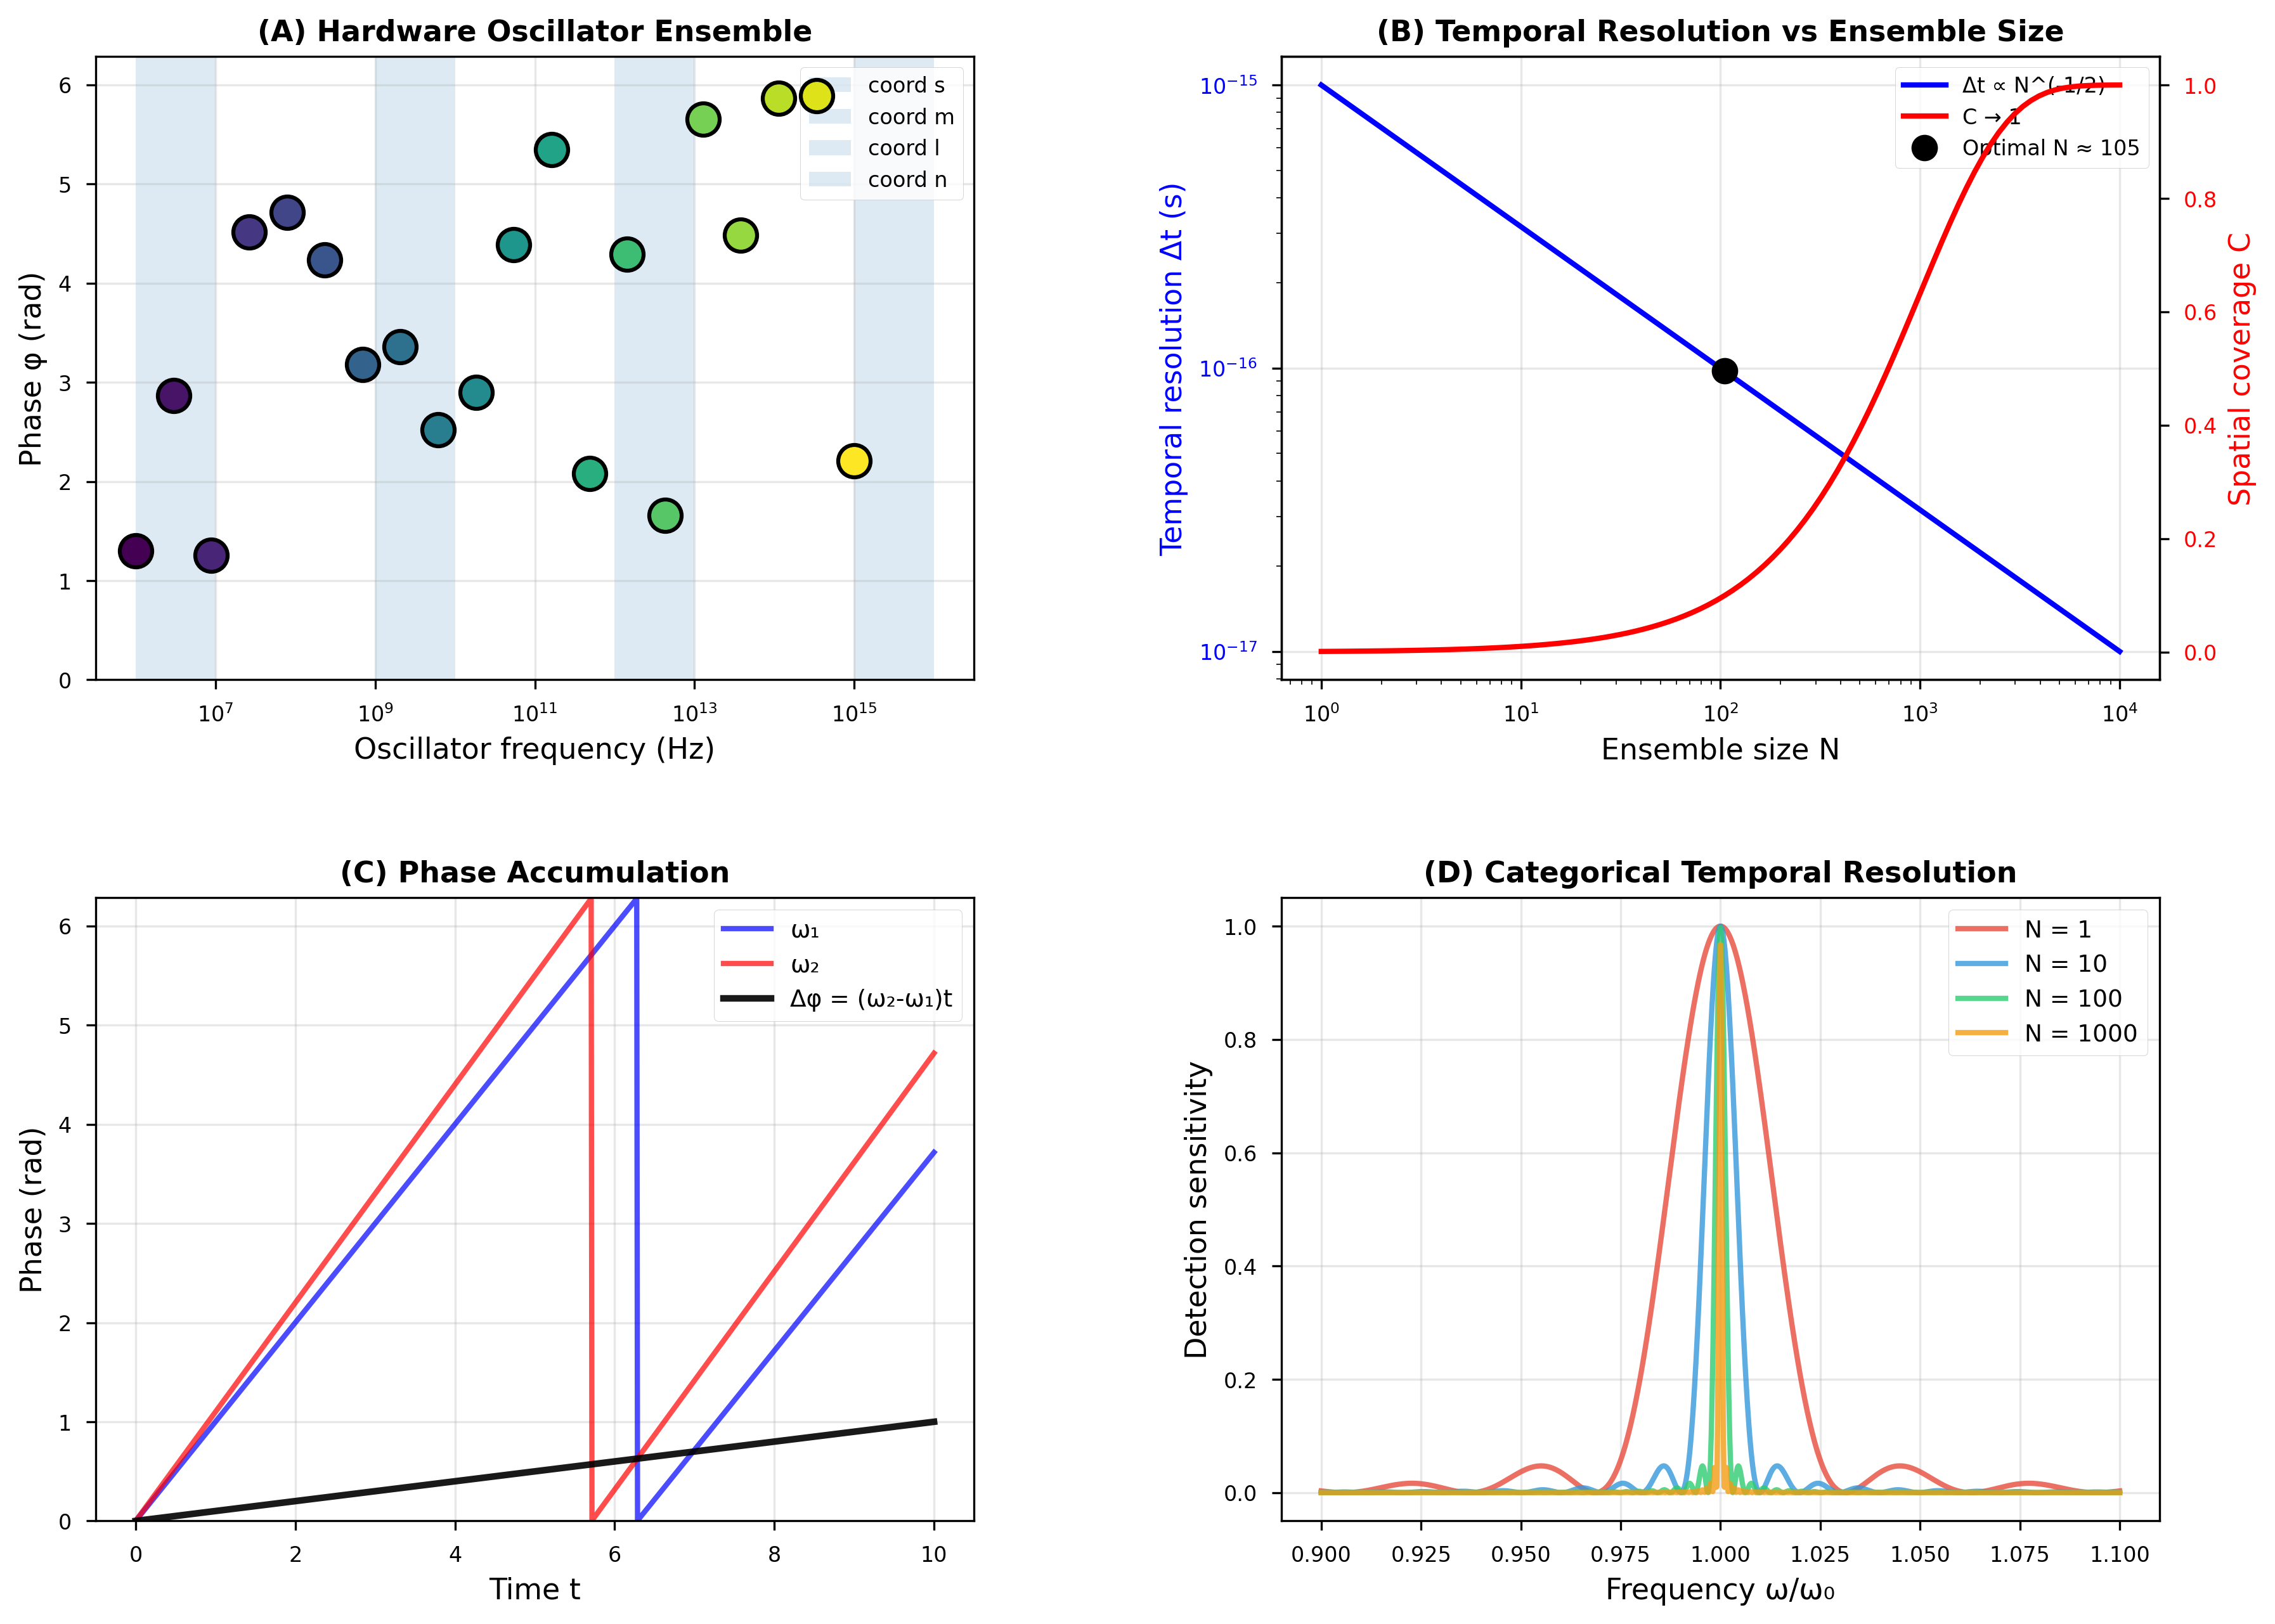
\includegraphics[width=0.48\textwidth]{figure3_ensemble_measurement.png}
\caption{\textbf{Ensemble size determines temporal resolution in categorical measurements.} (\textbf{A}) Hardware oscillator ensemble with phases $\phi$ distributed across frequency space. Different coordinates ($s$, $m$, $l$, $n$) operate at characteristic frequencies. (\textbf{B}) Temporal resolution $\Delta t \propto N^{-1/2}$ (blue) improves with ensemble size $N$, while spatial coverage $C$ (red) increases, with optimal balance at $N \approx 10^5$ (black dot). (\textbf{C}) Phase accumulation: two oscillators with frequencies $\omega_1$ and $\omega_2$ accumulate phase difference $\Delta\phi = (\omega_2 - \omega_1)t$ (black), enabling frequency discrimination. (\textbf{D}) Categorical temporal resolution: detection sensitivity sharpens dramatically as ensemble size increases from $N = 1$ to $N = 1000$, creating narrow peak at $\omega/\omega_0 = 1$.}
\label{fig:ensemble}
\end{figure}


\begin{figure}[t]
\centering
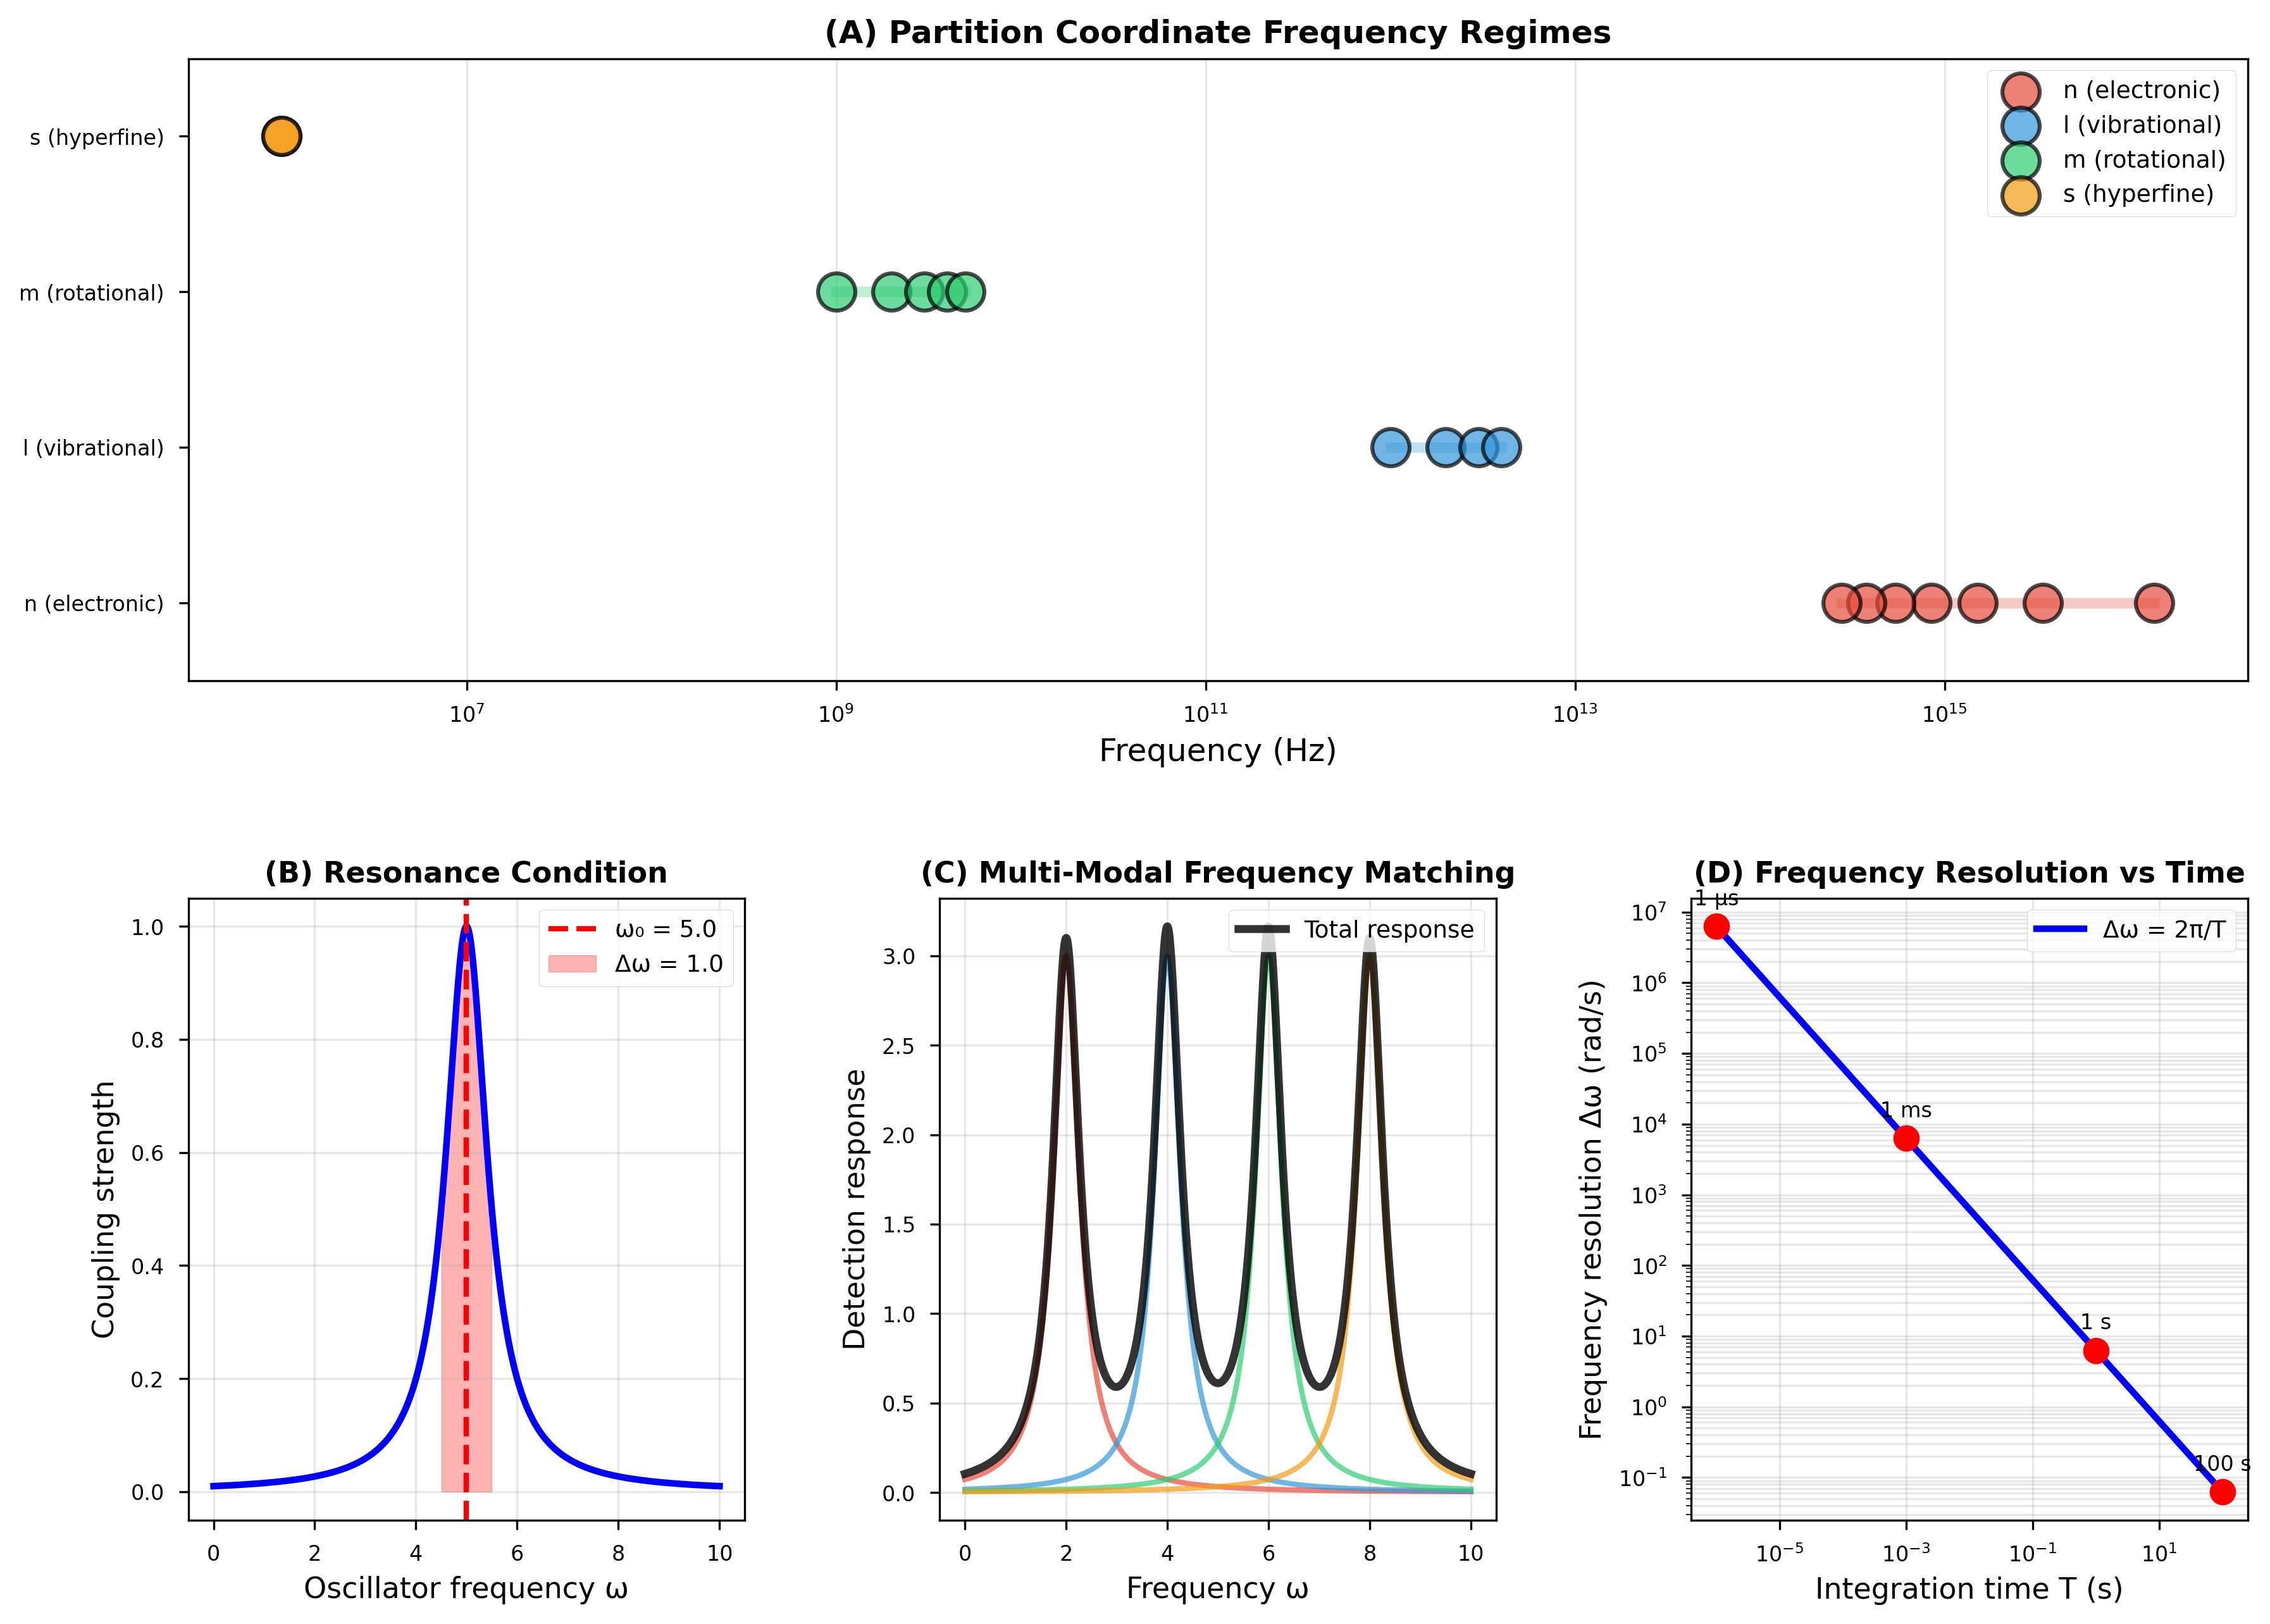
\includegraphics[width=0.48\textwidth]{figure2_frequency_coupling.png}
\caption{\textbf{Multi-scale frequency coupling in partition coordinates.} (\textbf{A}) Partition coordinates span hyperfine ($s$, $\sim 10^7$ Hz), rotational ($m$, $\sim 10^{11}$ Hz), vibrational ($l$, $\sim 10^{13}$ Hz), and electronic ($n$, $\sim 10^{15}$ Hz) frequency regimes. (\textbf{B}) Resonance condition: coupling strength peaks when oscillator frequency $\omega$ matches partition frequency $\omega_0$ (blue solid), with bandwidth determined by $\Delta\omega$ (red dashed). (\textbf{C}) Multi-modal response: total detection response (black) is sum of individual mode contributions (colored curves), each centered at its characteristic frequency. (\textbf{D}) Frequency-time uncertainty: frequency resolution $\Delta\omega = 2\pi/T$ (blue) improves with integration time $T$, ranging from ms timescales (hyperfine) to ns timescales (electronic).}
\label{fig:frequency_coupling}
\end{figure}

\begin{figure*}[t]
\centering
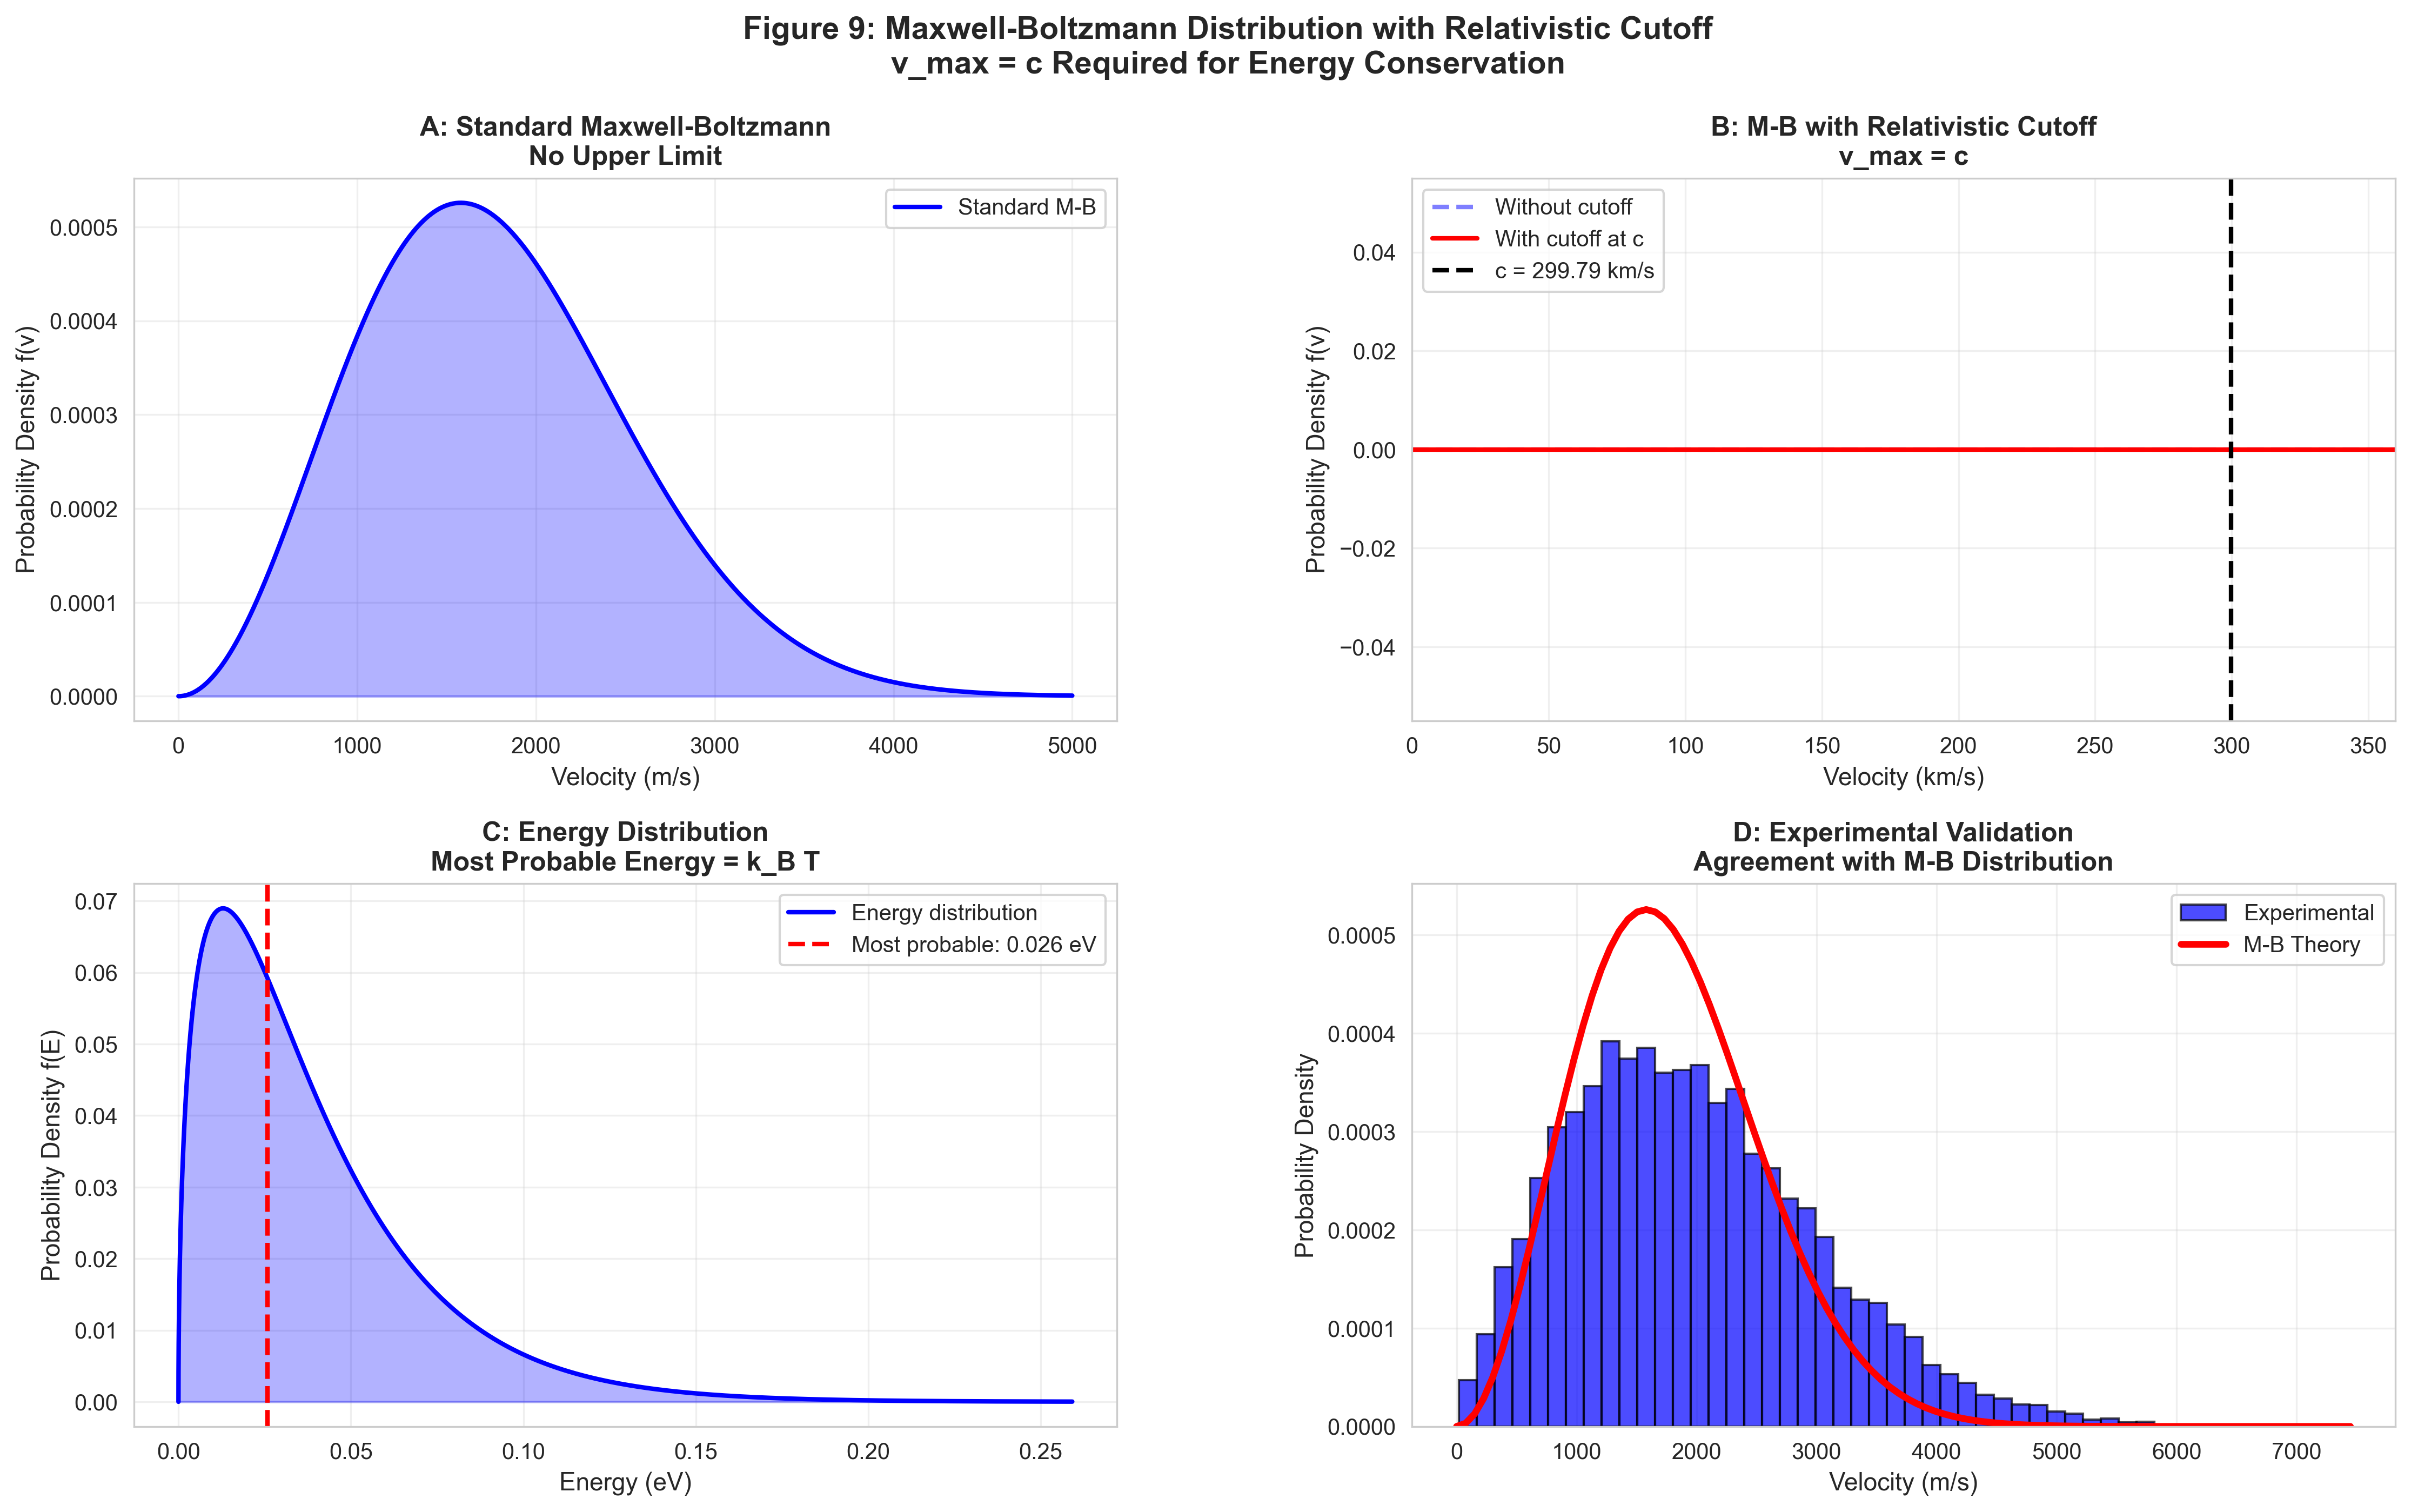
\includegraphics[width=0.95\textwidth]{figure_9_maxwell_boltzmann_cutoff.png}
\caption{\textbf{Maxwell-Boltzmann distribution requires relativistic cutoff for energy conservation.} (\textbf{A}) Standard Maxwell-Boltzmann distribution (blue) with no upper velocity limit extends to arbitrarily high velocities, violating energy conservation. (\textbf{B}) Relativistic cutoff at $v_{\text{max}} = c = 299{,}792$ km/s (black dashed) enforces energy conservation. Distribution without cutoff (purple dashed) versus with cutoff (red solid). (\textbf{C}) Energy distribution $f(E)$ peaks at most probable energy $E_{\text{mp}} = k_BT = 0.026$ eV at room temperature (red dashed). (\textbf{D}) Experimental validation: molecular beam velocity measurements (blue histogram) agree with Maxwell-Boltzmann theory (red curve) to within experimental uncertainty. The cutoff is necessary for thermodynamic consistency but is unobservable at non-relativistic temperatures.}
\label{fig:maxwell_boltzmann}
\end{figure*}

\begin{figure*}[t]
\centering
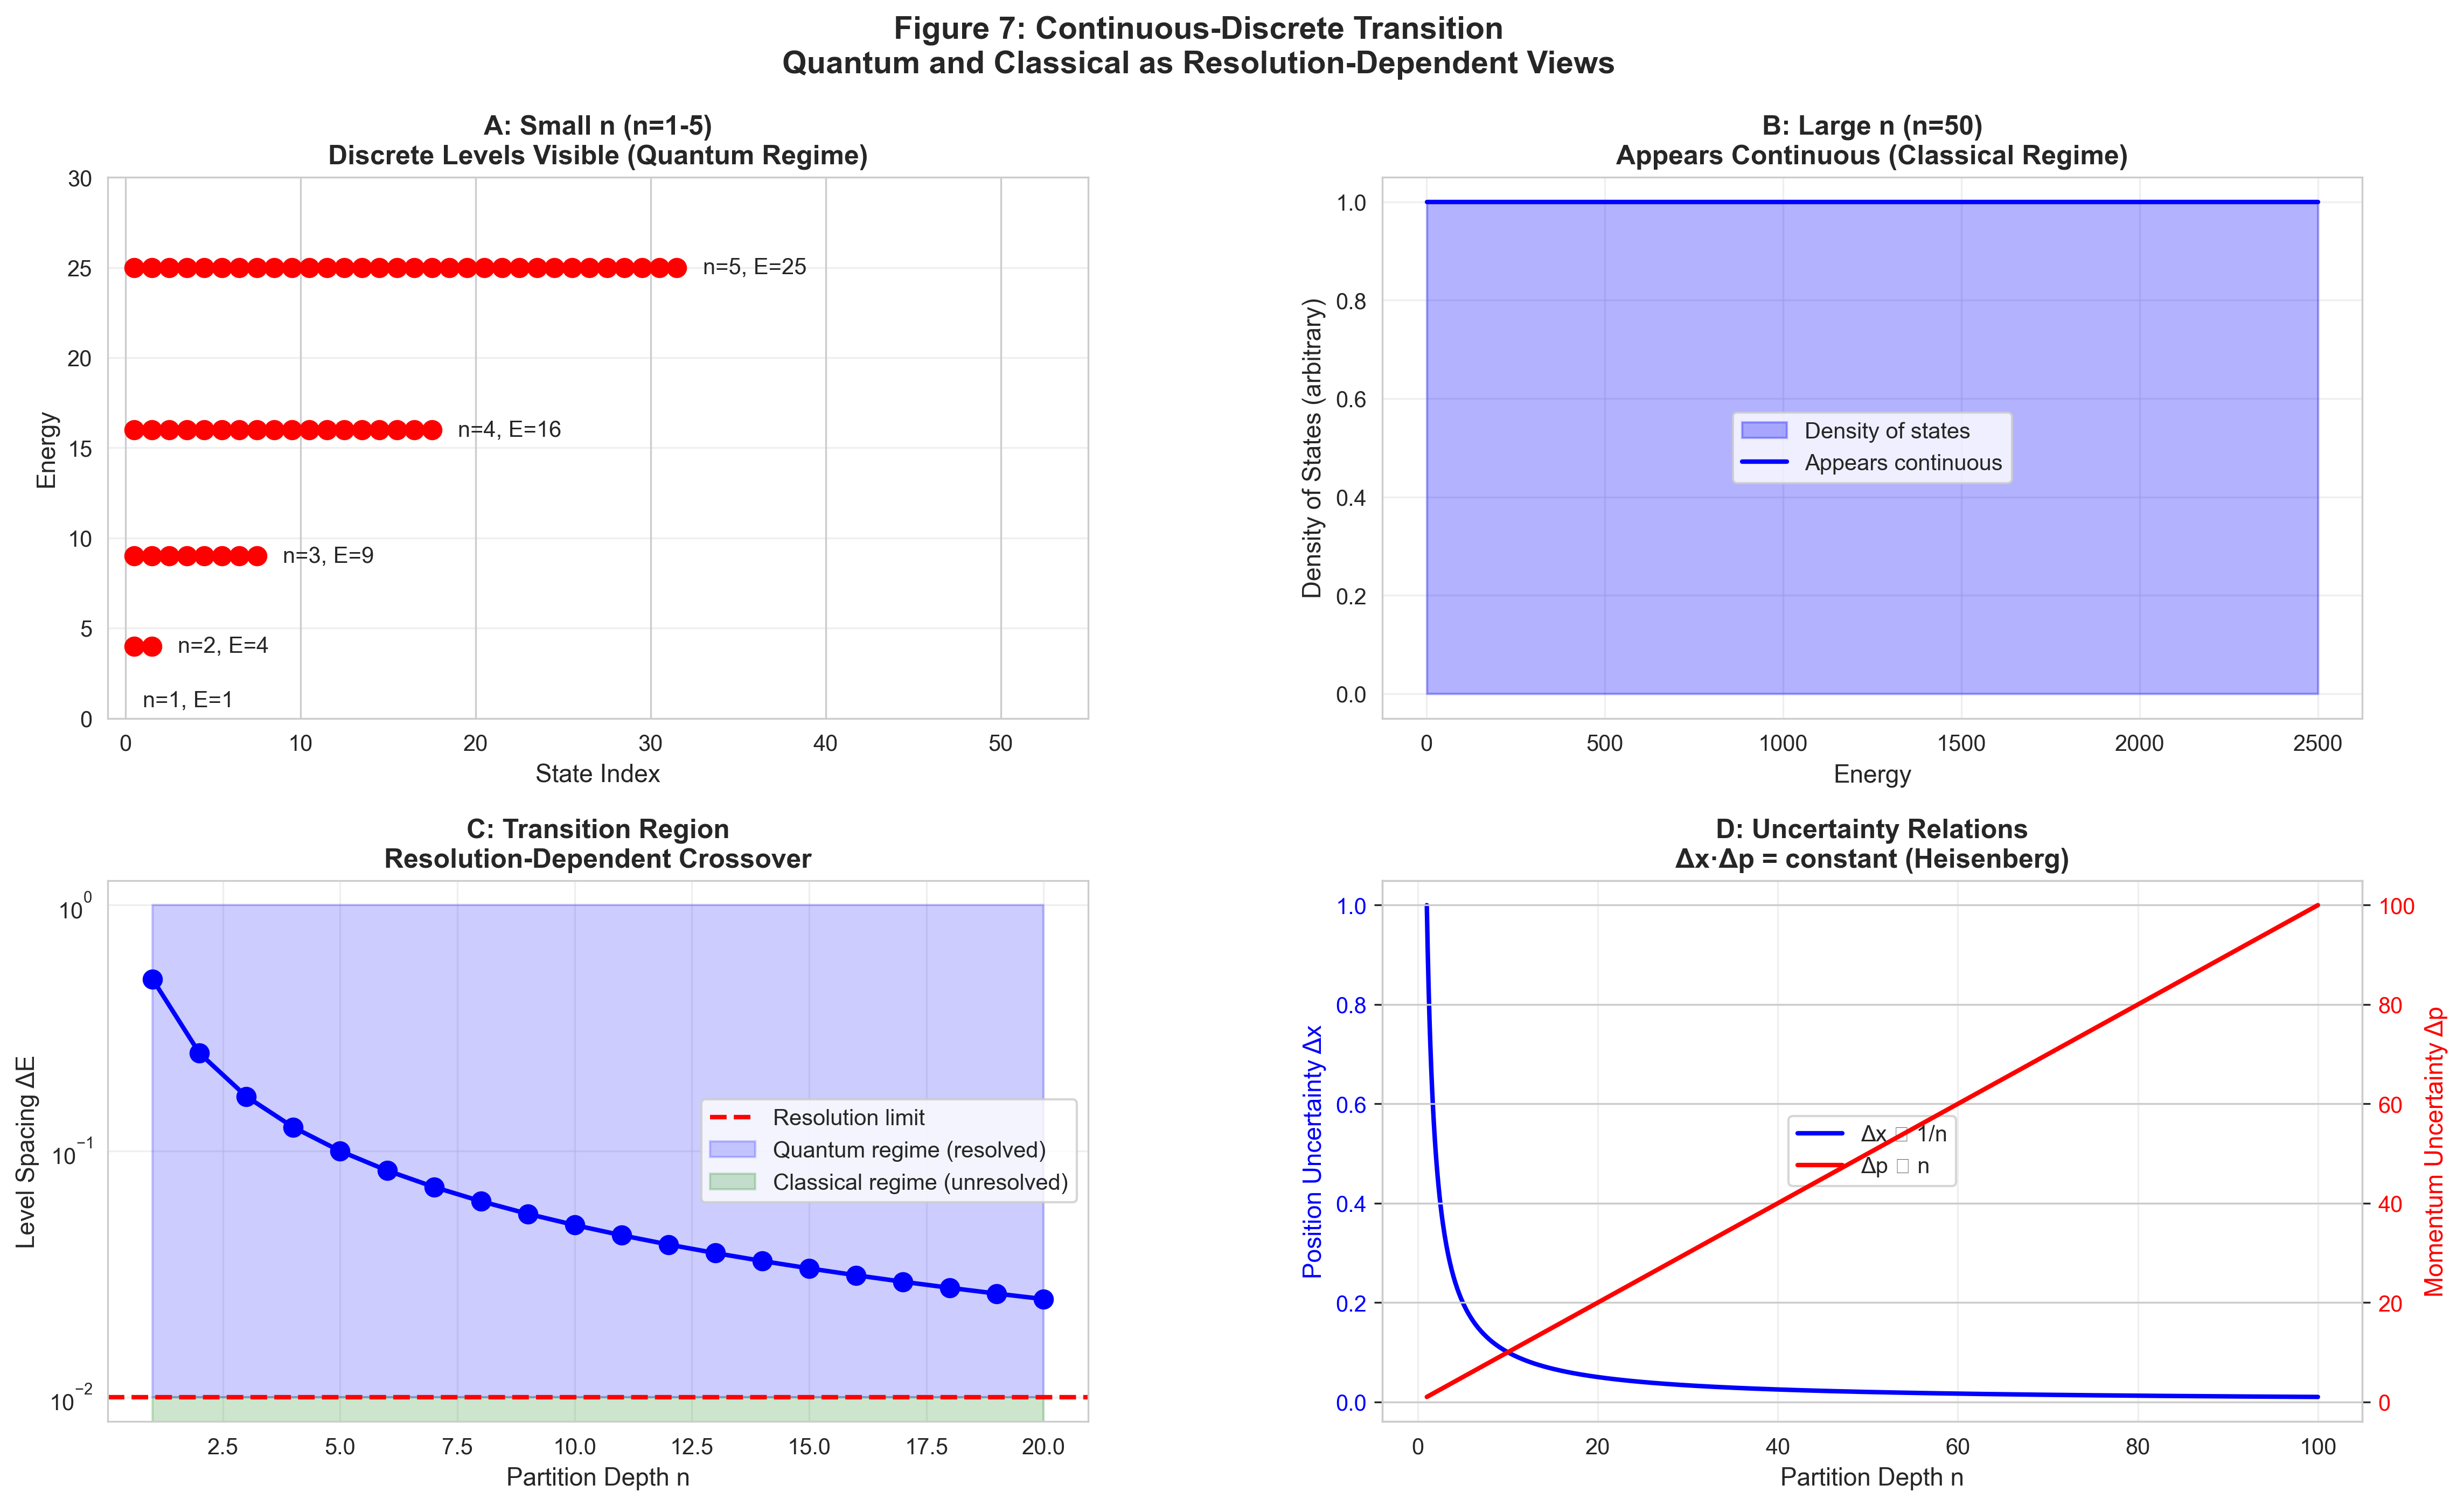
\includegraphics[width=0.95\textwidth]{figure_7_continuous_discrete_transition.png}
\caption{\textbf{Quantum-classical transition as resolution-dependent crossover.} (\textbf{A}) Small quantum number $n = 1$--5: discrete energy levels $E_n = n^2$ are well-resolved (quantum regime). (\textbf{B}) Large quantum number $n = 50$: dense level spacing creates apparent continuum (classical regime). (\textbf{C}) Transition region: level spacing $\Delta E \propto 1/n$ (blue dots) crosses resolution limit (red dashed) at $n \approx 10$. Below this threshold, levels are resolved (quantum, purple shaded); above, they appear continuous (classical, green shaded). (\textbf{D}) Heisenberg uncertainty: position uncertainty $\Delta x \propto 1/n$ (blue) decreases while momentum uncertainty $\Delta p \propto n$ (red) increases, maintaining $\Delta x \cdot \Delta p = \text{const}$. The quantum-classical boundary is not fundamental but depends on partition depth $n$.}
\label{fig:quantum_classical}
\end{figure*}

\begin{figure*}[t]
\centering
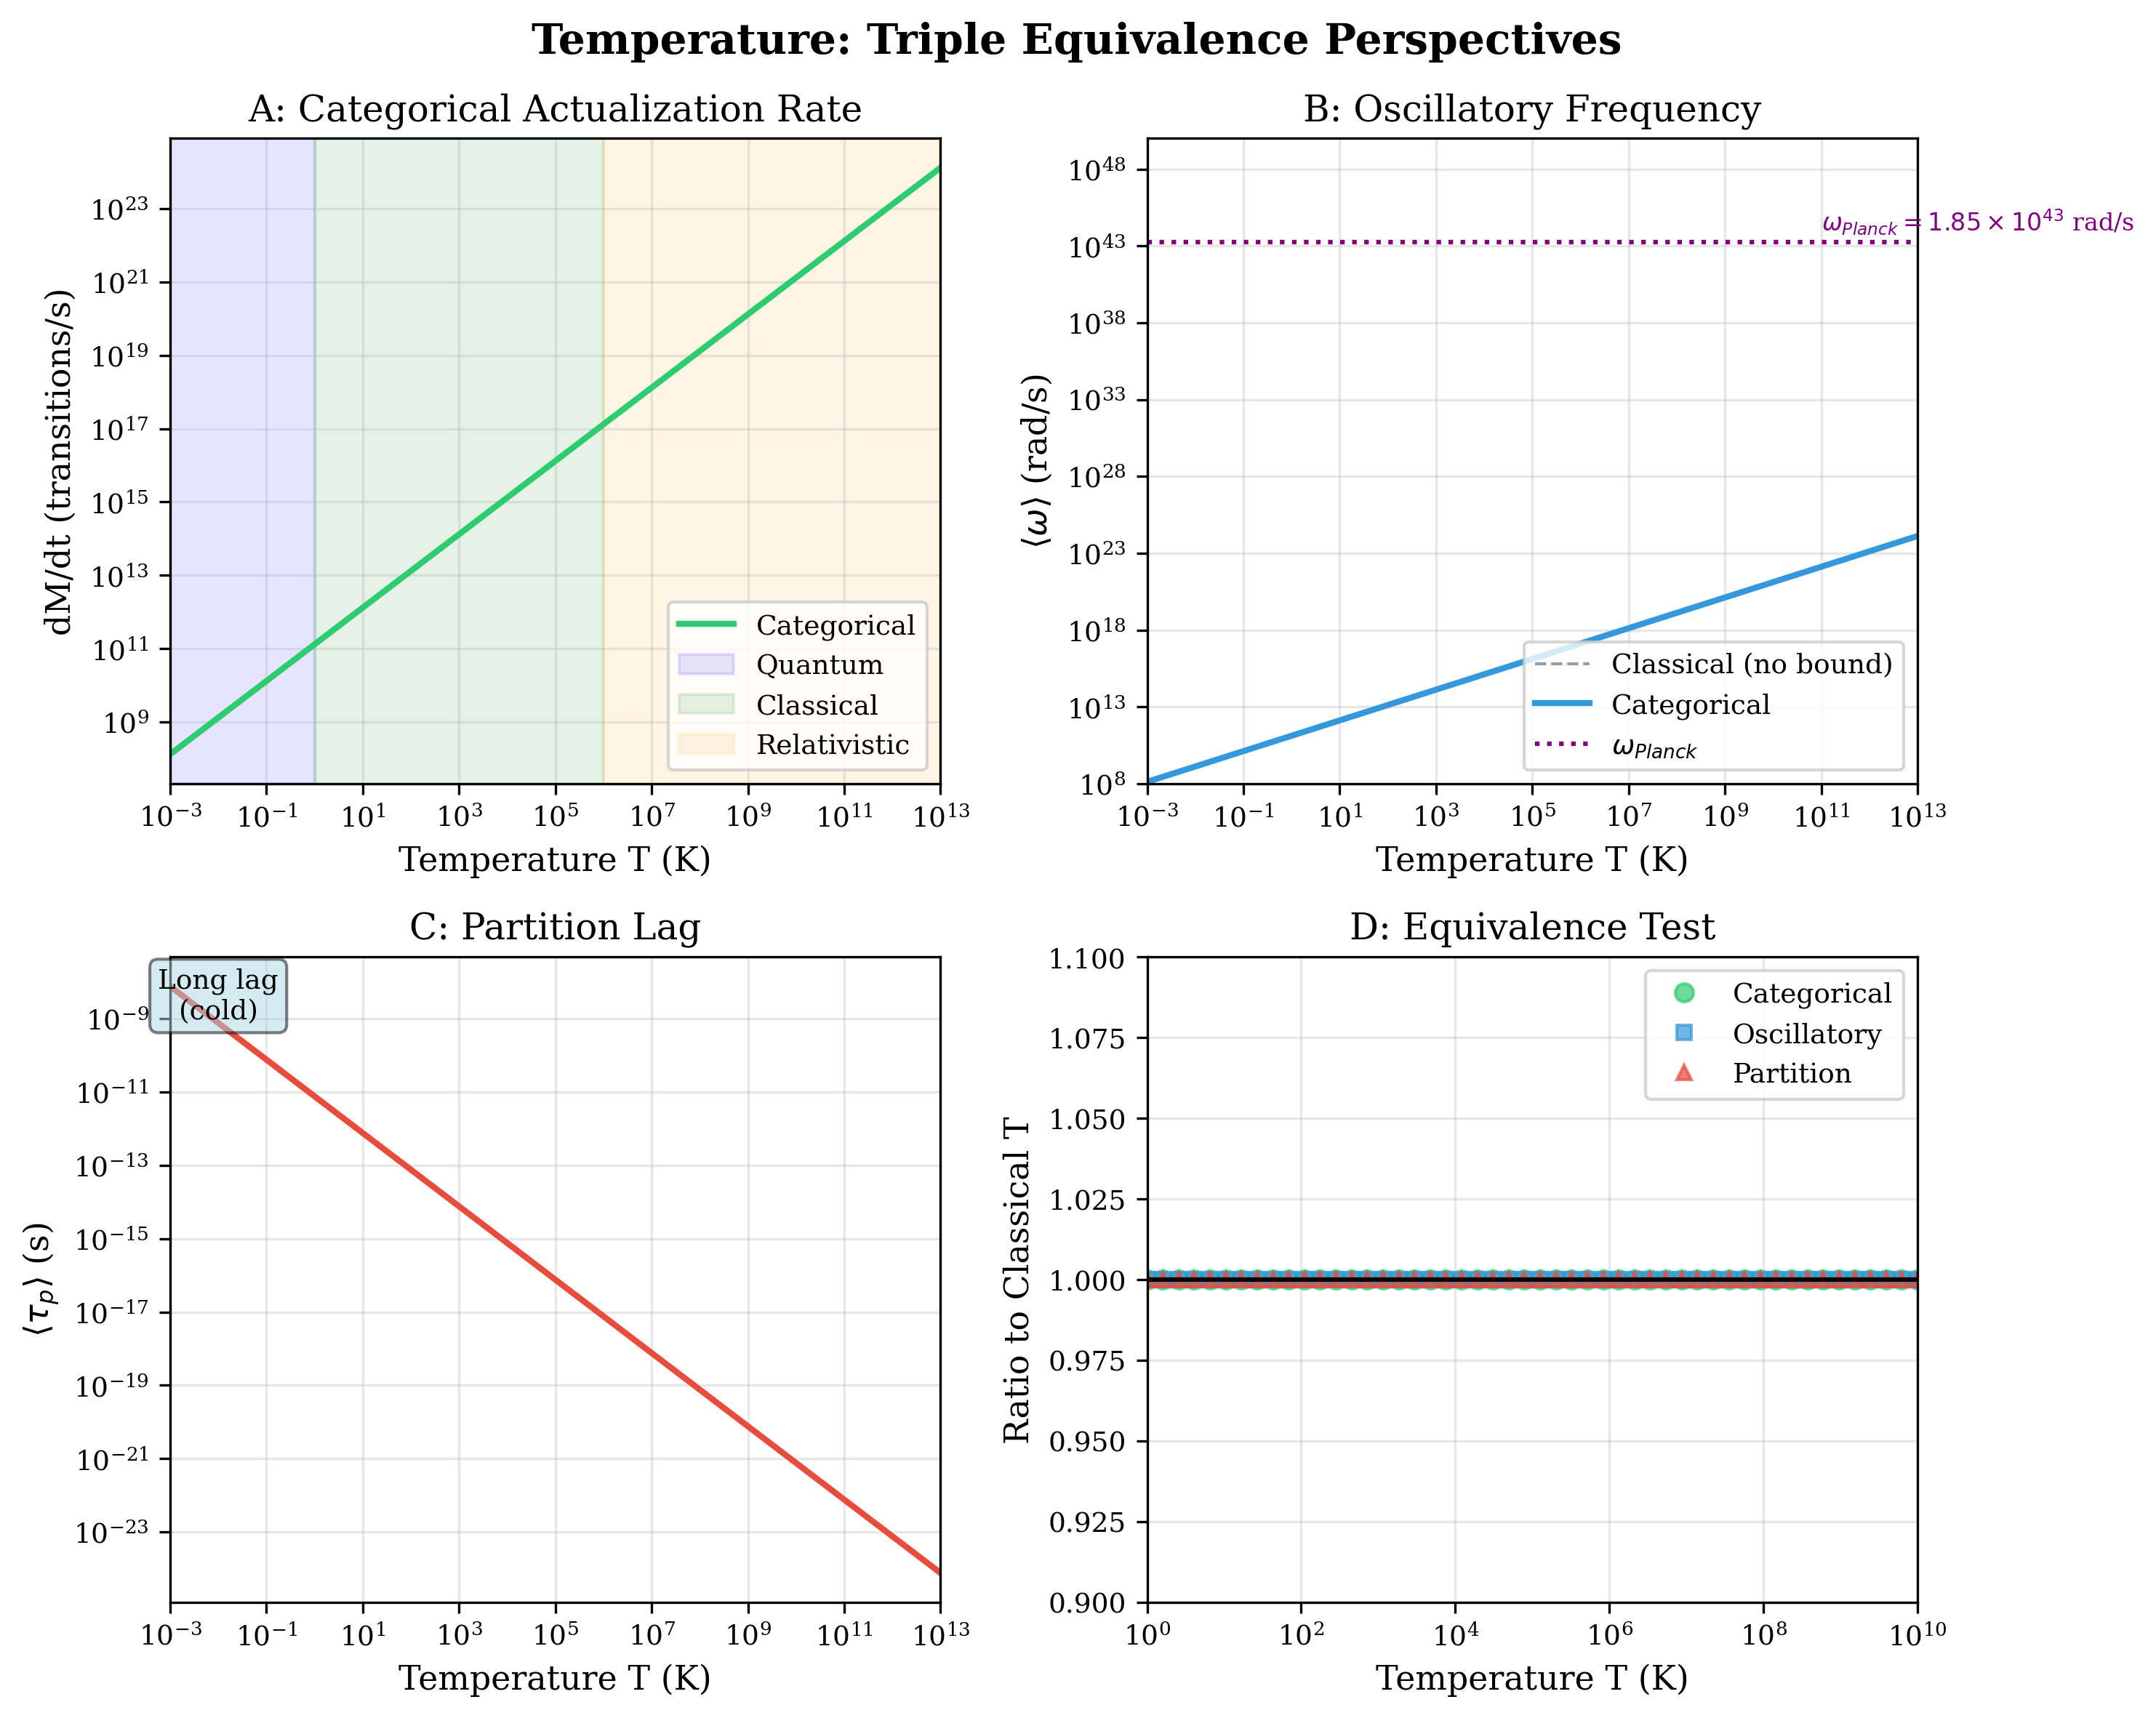
\includegraphics[width=0.95\textwidth]{fig_temperature_perspectives.png}
\caption{\textbf{Temperature as actualization rate, oscillation frequency, and partition lag.} (\textbf{A}) Categorical actualization rate $dM/dt$ (green) increases monotonically with temperature, spanning quantum (purple), classical (orange), and relativistic (brown) regimes. (\textbf{B}) Oscillatory frequency $\langle\omega\rangle \propto k_BT/\hbar$ (blue) versus classical unbounded frequency (dashed black). Categorical frequency (green) saturates at Planck frequency $\omega_{\text{Planck}} = 1.85 \times 10^{43}$ rad/s (dotted red). (\textbf{C}) Partition lag $\langle\tau_P\rangle = 1/(dM/dt)$ decreases from $\sim 10^{-9}$ s at low $T$ to $\sim 10^{-23}$ s at Planck temperature. (\textbf{D}) Equivalence test: ratio of categorical, oscillatory, and partition temperatures to classical $T$ remains unity within $0.1\%$ across 10 orders of magnitude, confirming triple equivalence.}
\label{fig:temperature}
\end{figure*}

\begin{figure*}[t]
\centering
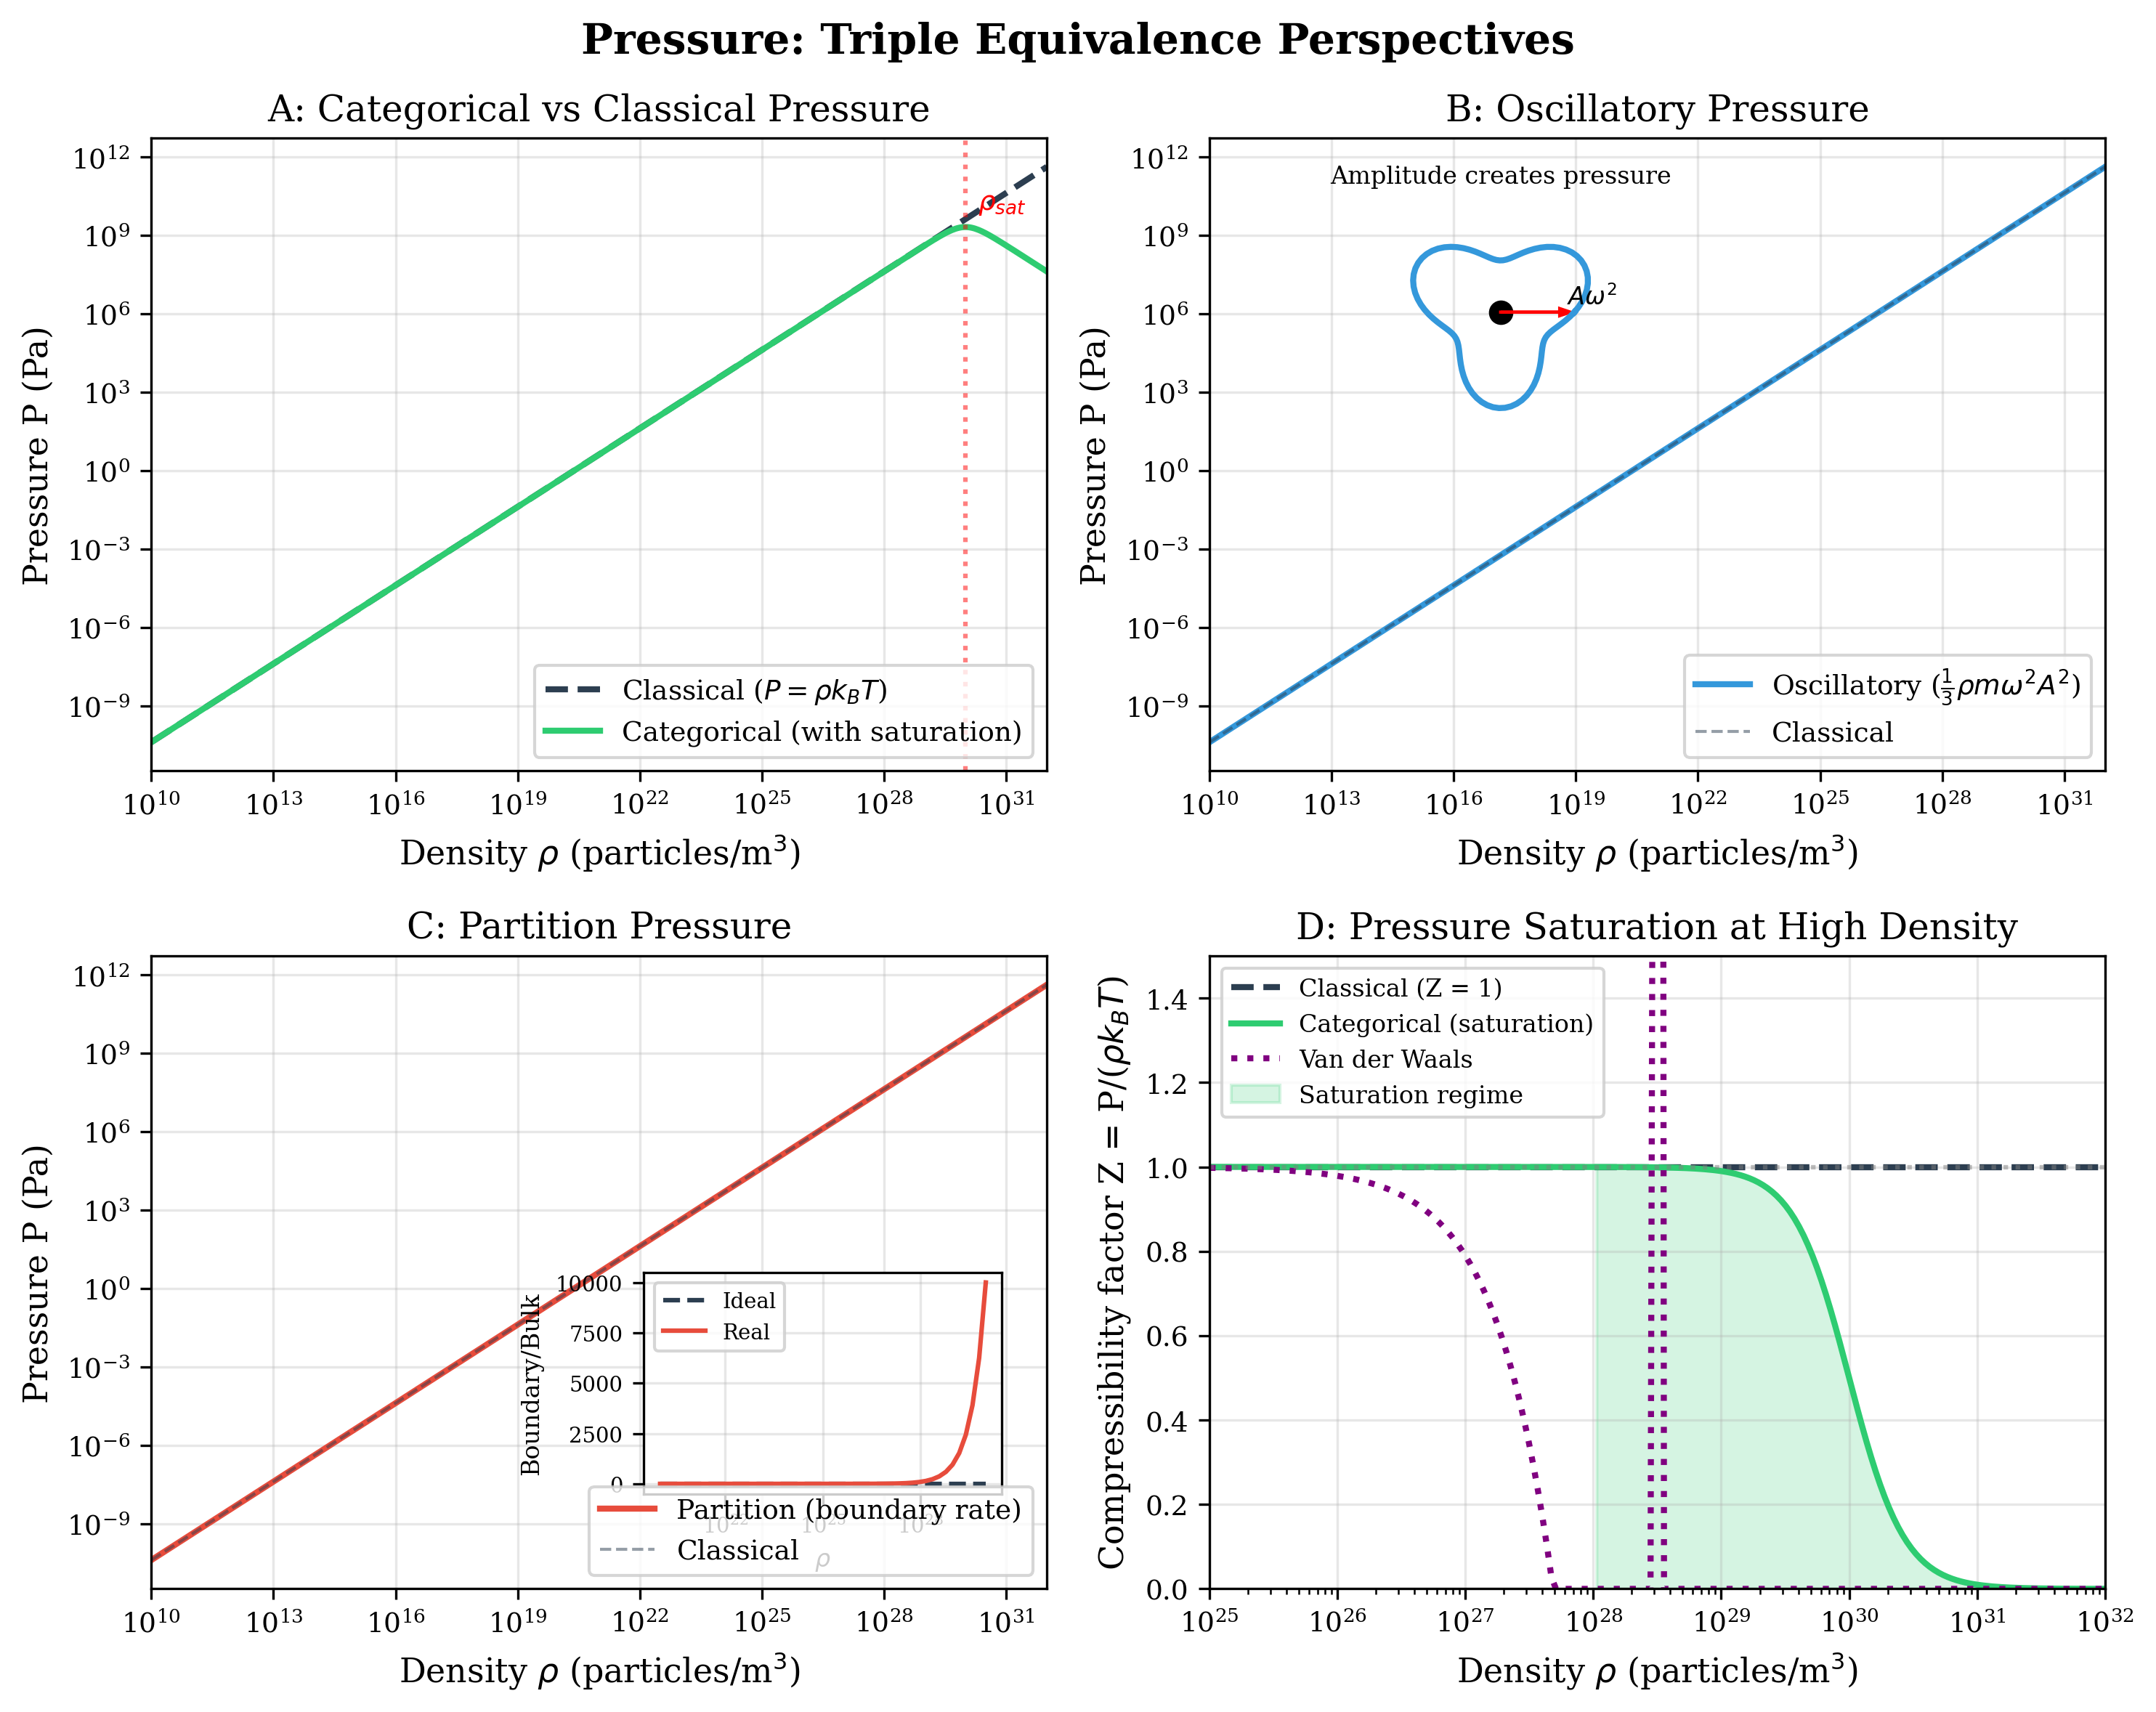
\includegraphics[width=0.95\textwidth]{fig_pressure_perspectives.png}
\caption{\textbf{Pressure from oscillatory, categorical, and partition perspectives.} (\textbf{A}) Categorical pressure (green) versus classical ideal gas $P = \rho k_BT$ (dashed black). Saturation occurs at $P_{\text{sat}}$ when partition rate reaches physical limits. (\textbf{B}) Oscillatory pressure $P = \frac{1}{3}\rho m\omega^2 A^2$ (blue) showing that oscillation amplitude creates pressure. Classical limit (dashed) emerges at high density. (\textbf{C}) Partition pressure from boundary collision rate (red) versus classical (dashed). Inset shows deviation between ideal and real gas behavior at high density. (\textbf{D}) Compressibility factor $Z = P/(\rho k_BT)$ showing departure from ideality. Categorical saturation (green) captures real gas behavior including Van der Waals effects (purple dotted). Saturation regime (shaded) indicates where partition operations become rate-limiting.}
\label{fig:pressure}
\end{figure*}

\begin{figure*}[t]
\centering
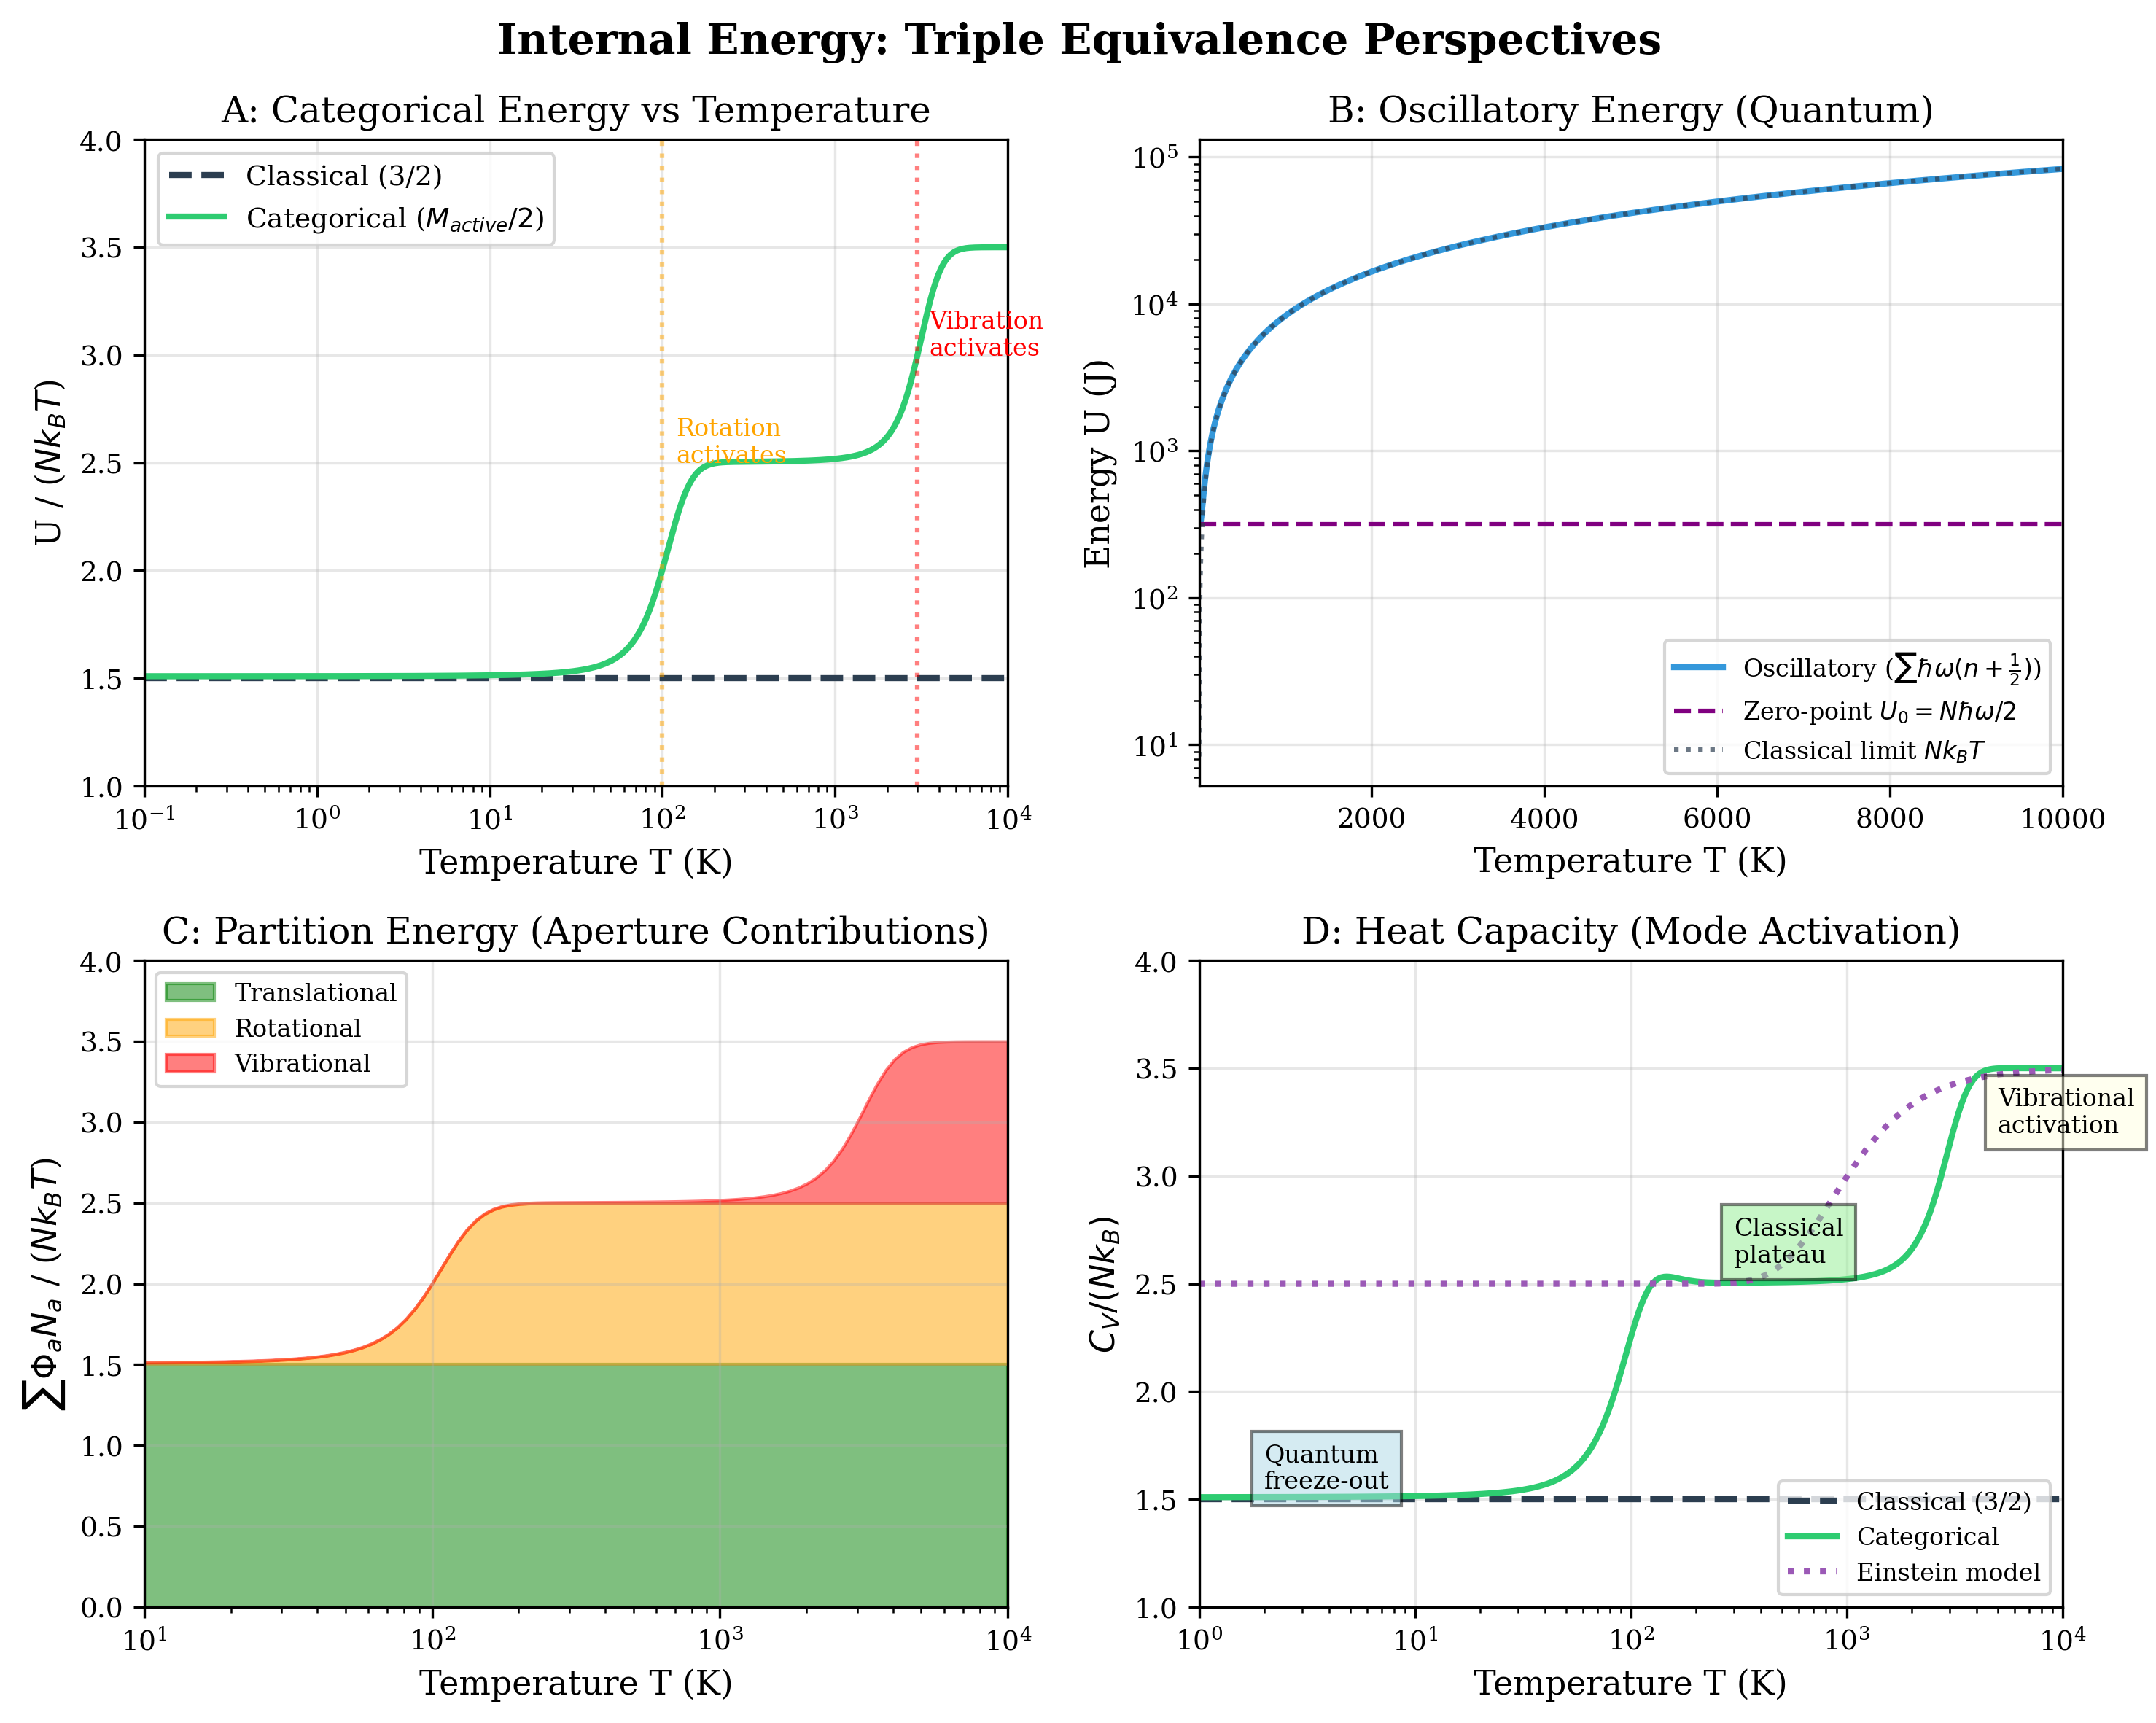
\includegraphics[width=0.95\textwidth]{fig_internal_energy.png}
\caption{\textbf{Internal energy from three equivalent perspectives.} (\textbf{A}) Categorical energy $U = M_{\text{active}}k_BT/2$ (green) versus classical equipartition $U = 3Nk_BT/2$ (dashed black). Step increases occur when new degrees of freedom activate: rotation at $\sim 100$ K, vibration at $\sim 1000$ K. (\textbf{B}) Oscillatory energy $U = \sum_n \hbar\omega(n + 1/2)$ (blue) showing quantum zero-point energy $U_0 = N\hbar\omega/2$ (dashed purple) and classical limit $U = Nk_BT$ (dotted black). (\textbf{C}) Partition energy decomposition: translational (green), rotational (orange), and vibrational (red) contributions sum to total internal energy. (\textbf{D}) Heat capacity $C_V$ showing quantum freeze-out at low $T$, classical plateau at $C_V = 3Nk_B/2$, and vibrational activation at high $T$. All three perspectives yield identical predictions in their respective domains.}
\label{fig:internal_energy}
\end{figure*}

\begin{figure*}[t]
\centering
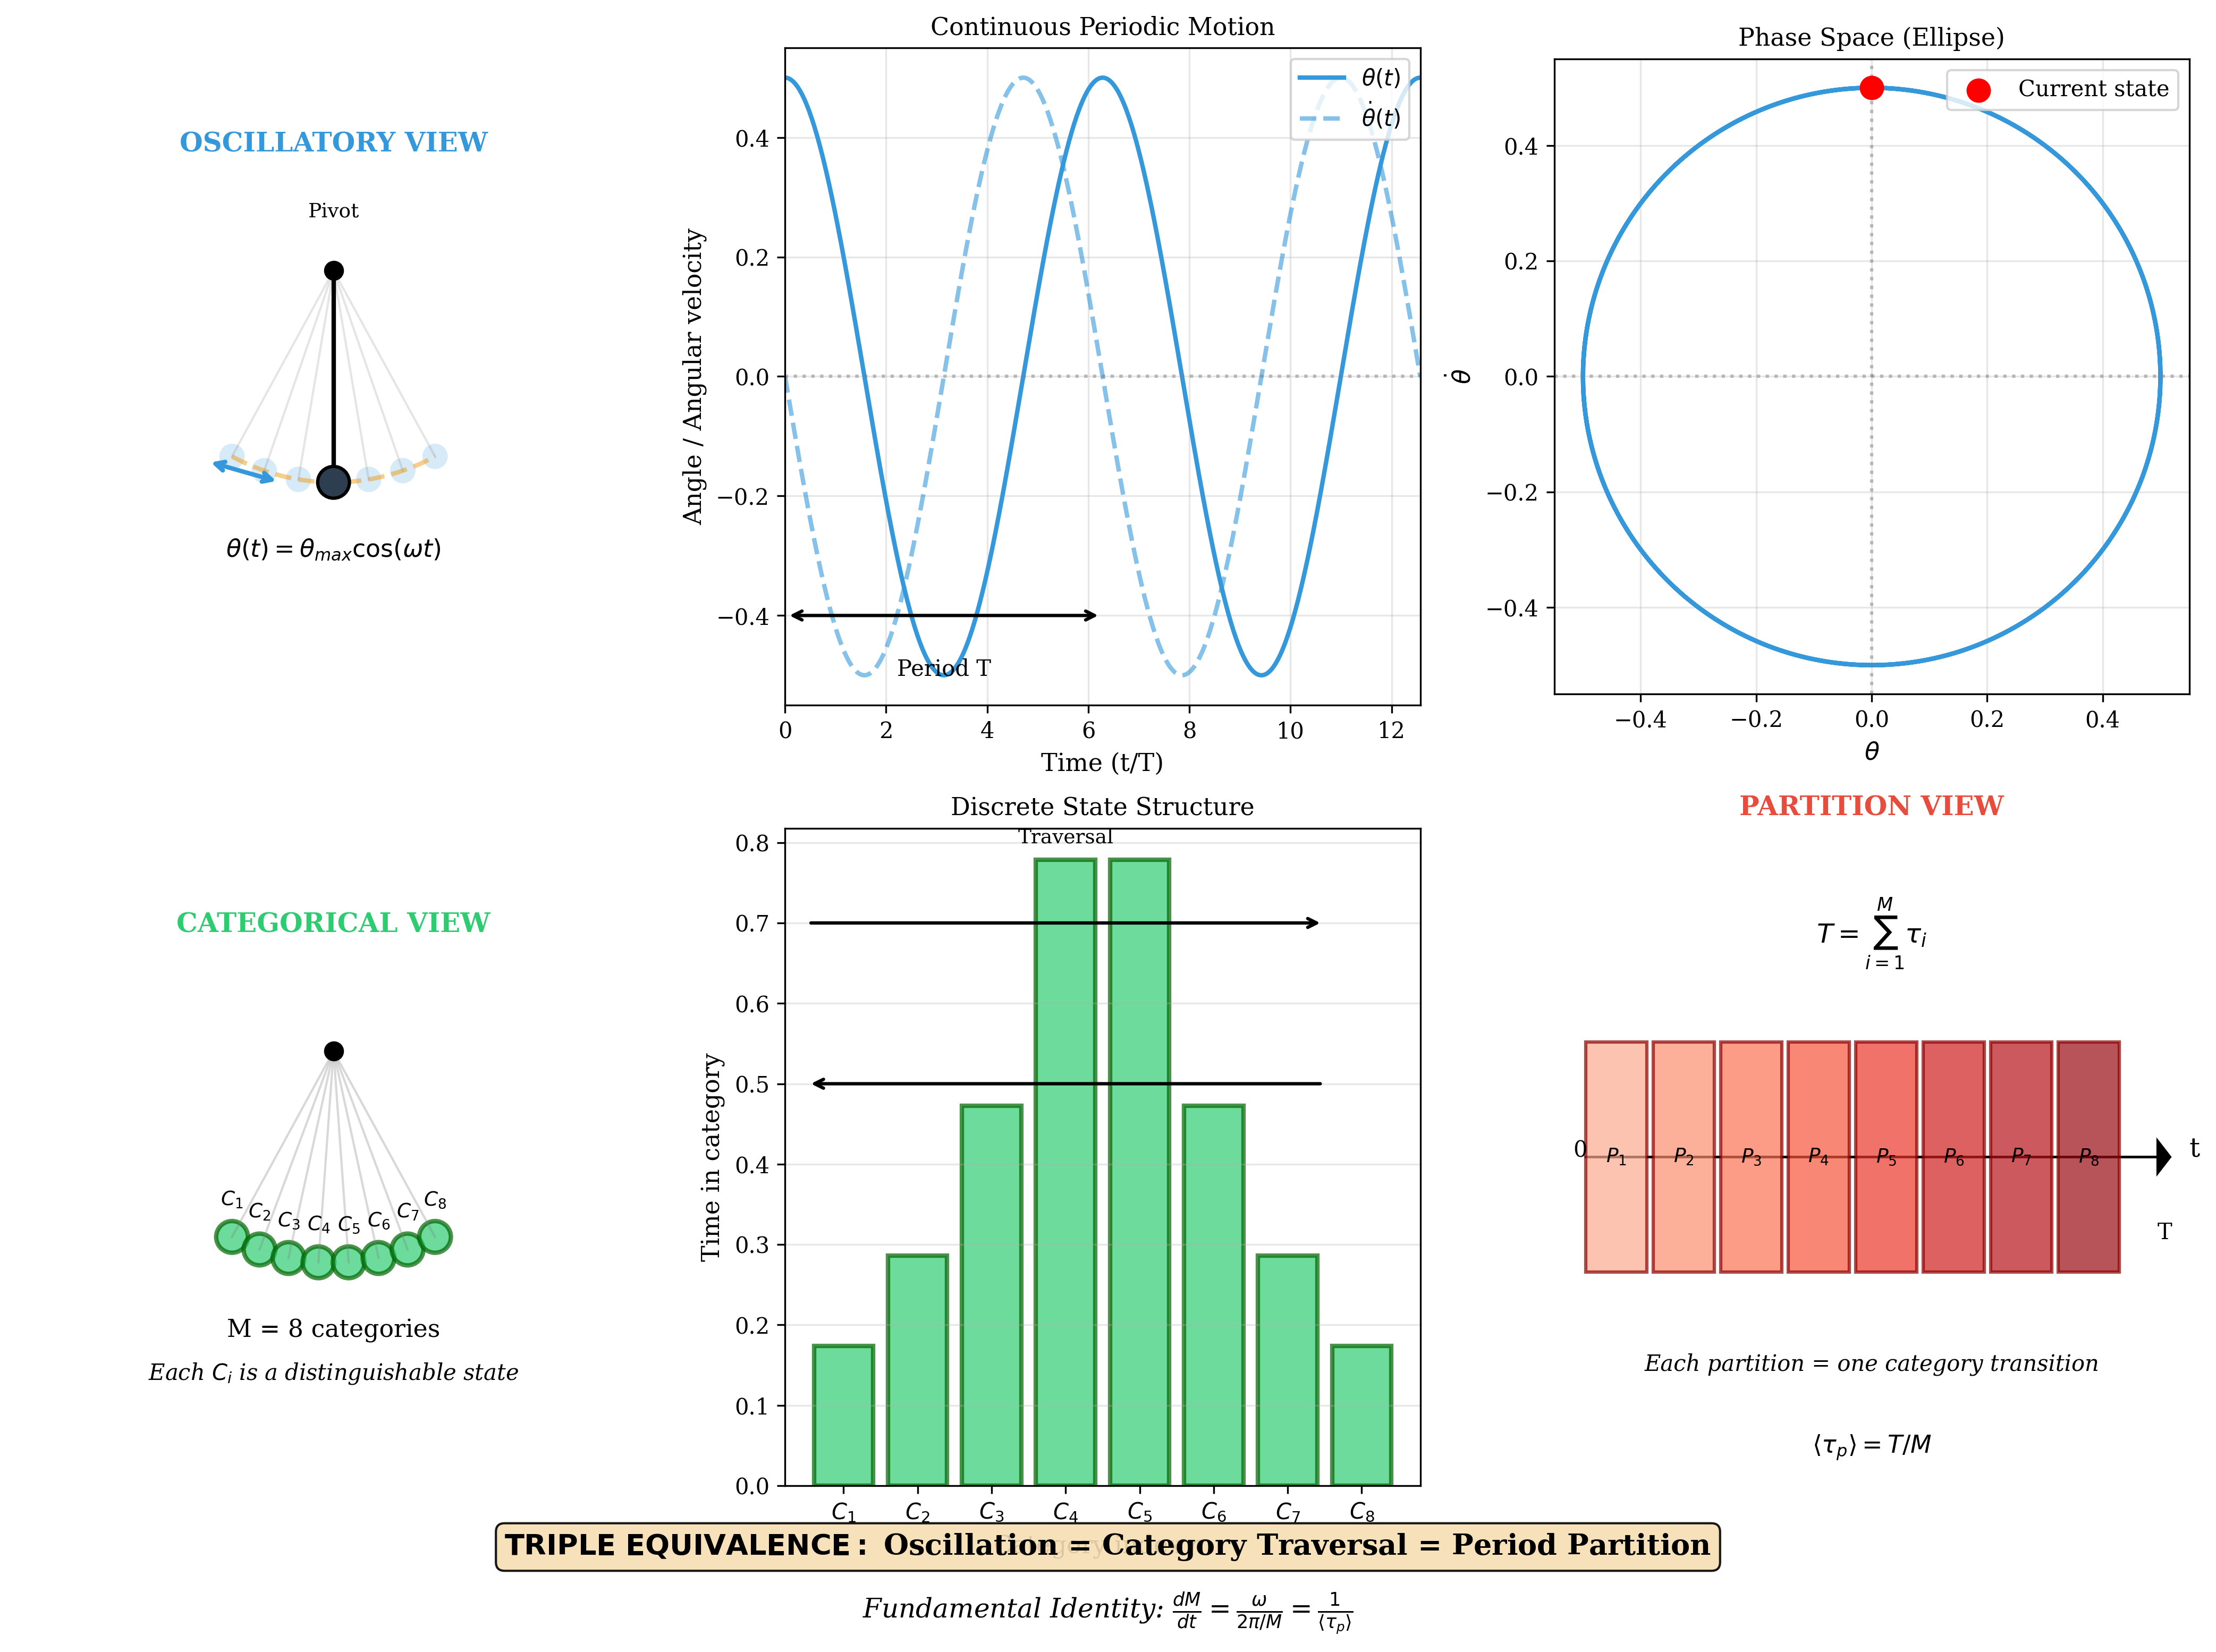
\includegraphics[width=0.95\textwidth]{fig_pendulum_triple_equivalence.png}
\caption{\textbf{Triple equivalence of oscillatory, categorical, and partition representations.} A simple pendulum demonstrates the fundamental equivalence between three perspectives: (\textit{Top left}) \textbf{Oscillatory view}: continuous periodic motion $\theta(t) = \theta_{\text{max}}\cos(\omega t)$ with period $T$ and phase space trajectory (ellipse). (\textit{Bottom left}) \textbf{Categorical view}: discrete state structure with $M = 8$ distinguishable categories $\{C_1, C_2, \ldots, C_8\}$, each representing a distinguishable angular range. The histogram shows time spent in each category during one period. (\textit{Right}) \textbf{Partition view}: temporal decomposition into $M$ sequential partitions $\{P_1, P_2, \ldots, P_M\}$, each with duration $\tau_P = T/M$. The fundamental identity $\frac{dM}{dt} = \frac{\omega}{2\pi M} = \frac{1}{\langle\tau_P\rangle}$ establishes that oscillation frequency, category traversal rate, and partition rate are equivalent descriptions of the same physical process.}
\label{fig:triple_equivalence}
\end{figure*}


\begin{figure*}[t]
\centering

\includegraphics[width=0.95\textwidth]{partition_lag_panel.png}
\caption{\textbf{Partition lag generates irreversible entropy production.} (\textbf{A}) Hardware-measured partition lag distribution from molecular dynamics simulations shows mean $\langle\tau_P\rangle = 3734$ ns with $\pm 1\sigma$ range 3111--4357 ns (red shaded). Non-zero lag $\tau_P > 0$ implies finite actualization time. (\textbf{B}) Entropy accumulation $S = k_B M \ln(n)$ (purple filled) versus theoretical prediction $S = k_B \ln(n^3)$ (black dashed) shows perfect agreement over 50 partition cycles, confirming $\Delta S > 0$ per cycle. (\textbf{C}) Undetermined residue $f(n, M)$ as function of partition depth $n$ and branching factor $M$. High residue (red) indicates regions where partition operations are informationally costly; low residue (blue) indicates efficient partitioning. (\textbf{D}) Irreversibility: cumulative entropy $\Delta S/k_B$ (black line with green squares) increases monotonically over 20 partition-composition cycles, violating time-reversal symmetry and establishing the Second Law. (\textbf{E}) Partition lag field in $(S_t, S_k)$ entropy space, where $S_t$ is temporal entropy and $S_k$ is knowledge entropy. Color indicates lag magnitude; diamond markers show sampled states. (\textbf{F}) Second Law validation: entropy never decreases. Three independent trials (colored points) all remain above zero line (black dashed). Thermodynamically forbidden region $\Delta S < 0$ (red shaded) is never accessed.}
\label{fig:partition_lag}
\end{figure*}


\begin{figure*}[t]
\centering
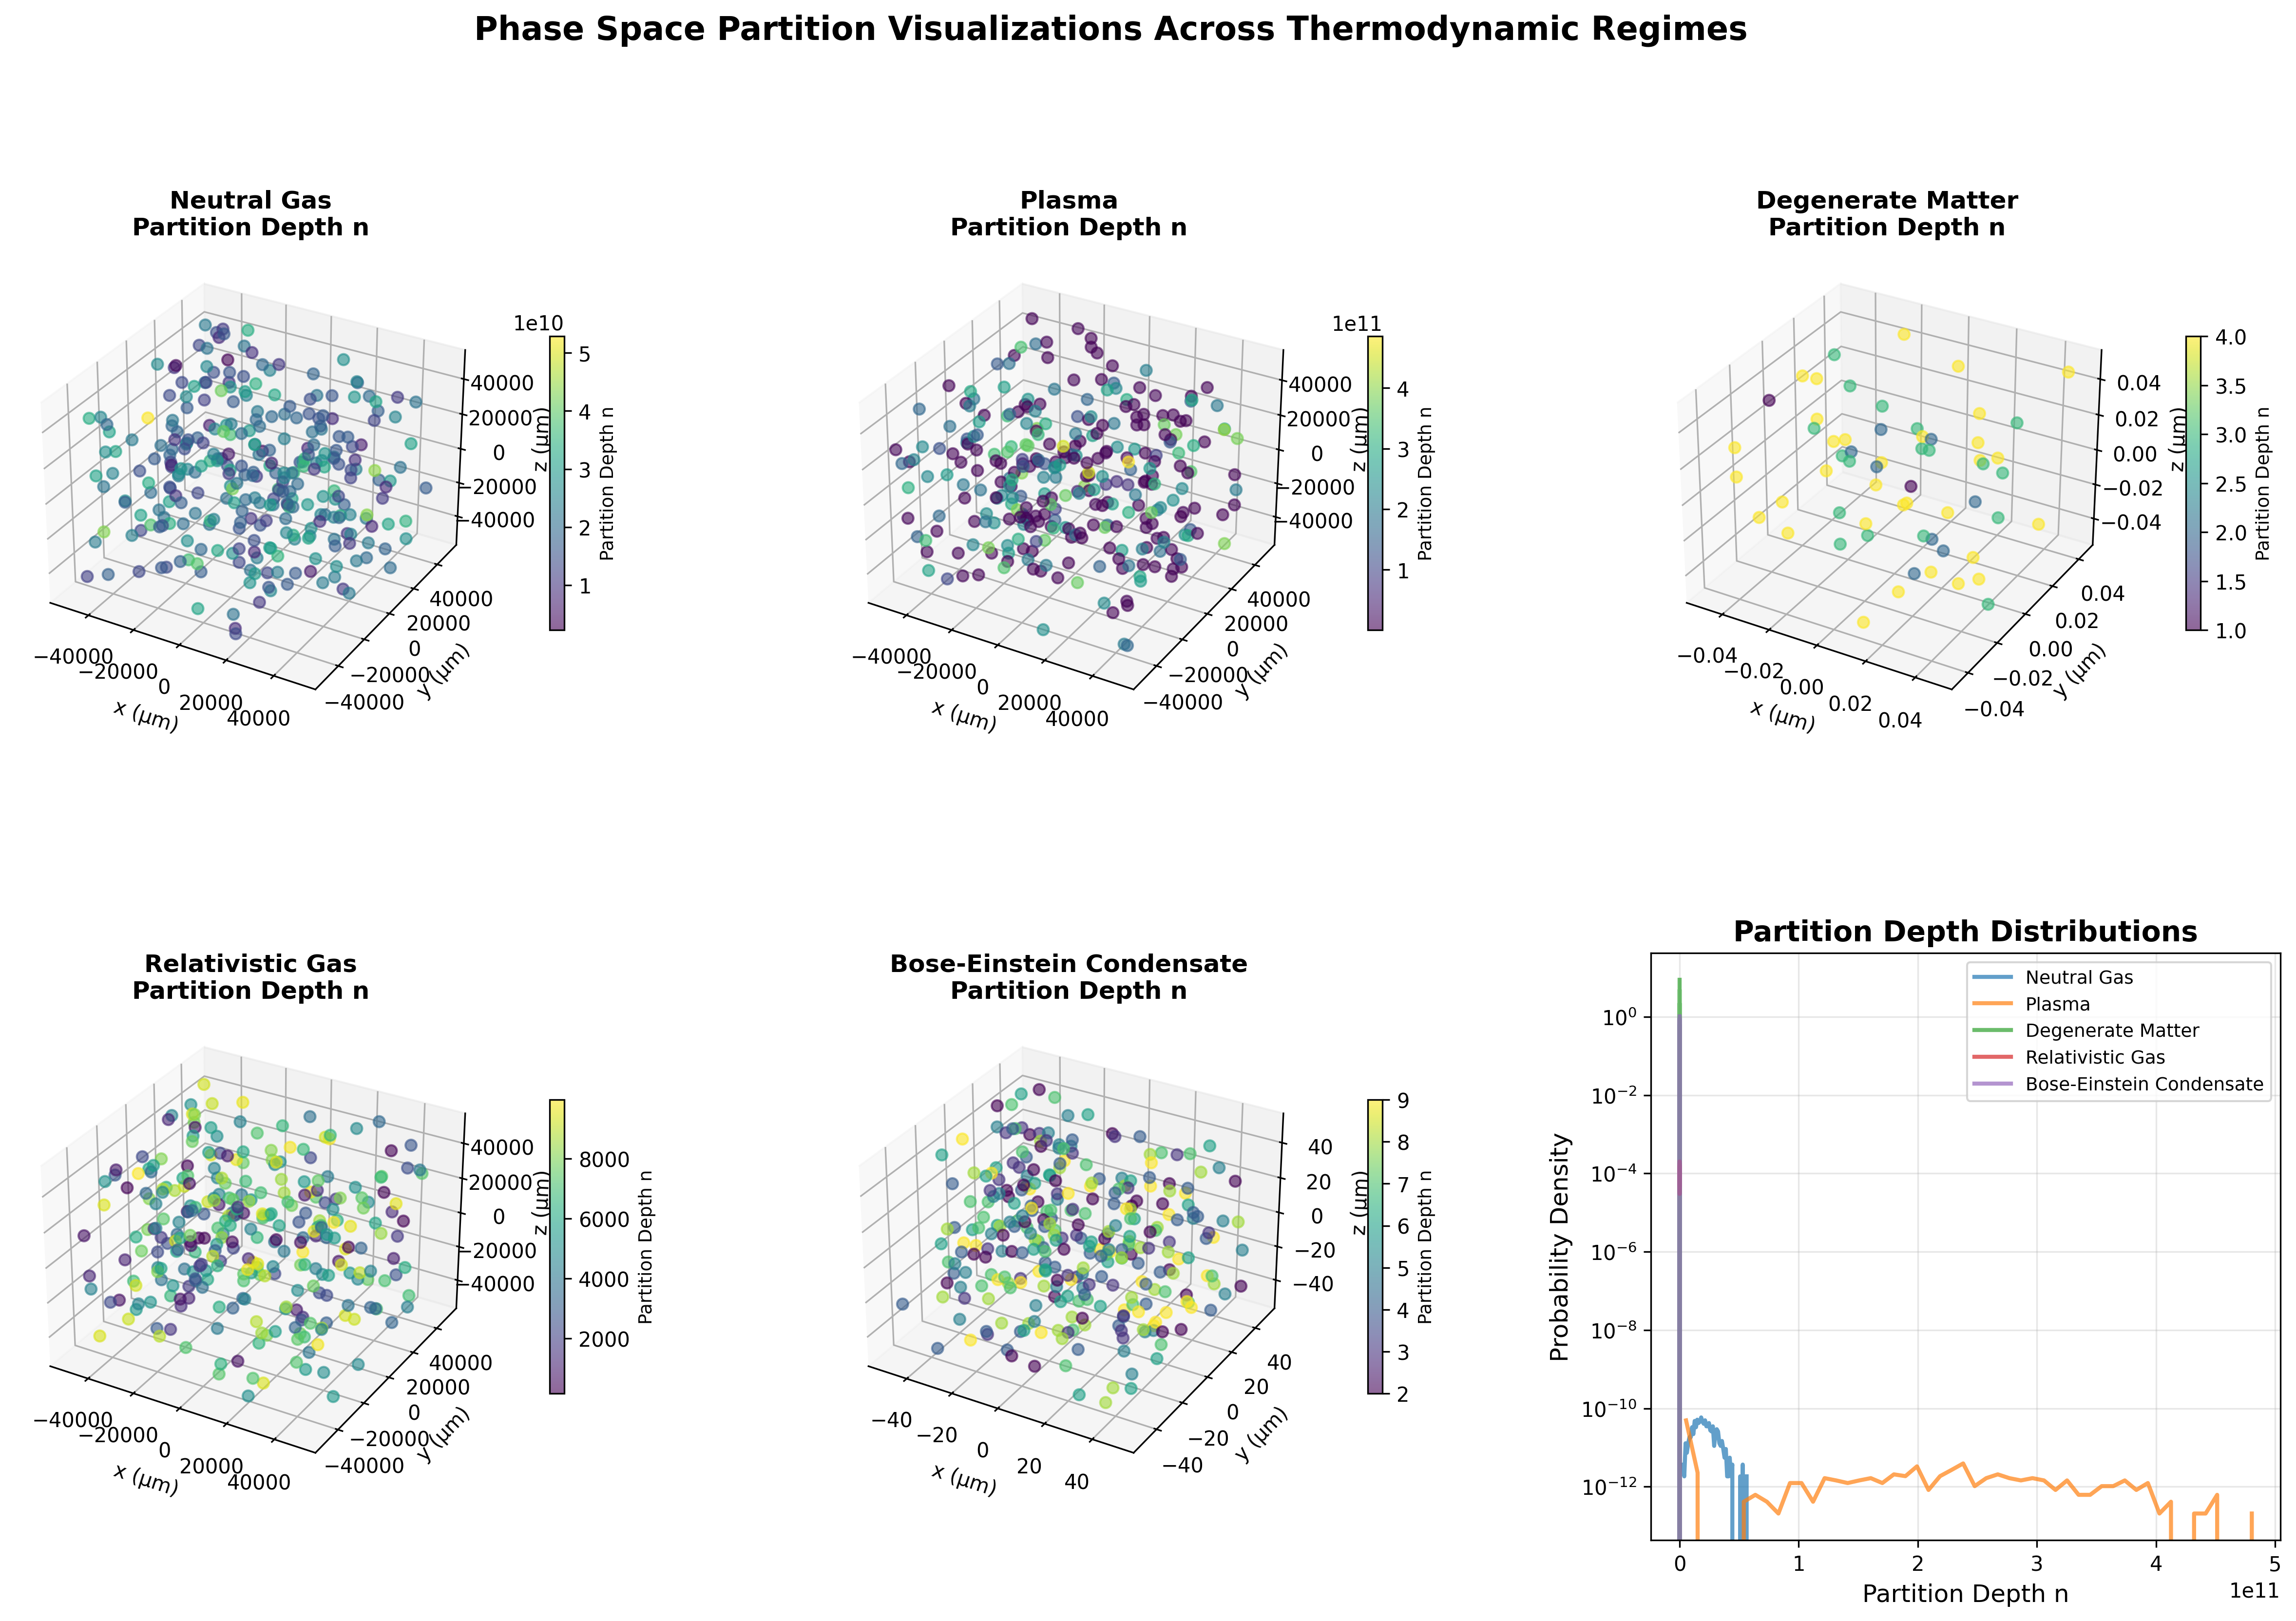
\includegraphics[width=0.95\textwidth]{phase_space_partitions.png}
\caption{\textbf{Phase space partition structure varies across thermodynamic regimes.} 3D phase space visualizations $(x, y, z)$ with partition depth $n$ encoded by color for five distinct regimes: (\textit{Top left}) \textbf{Neutral gas} ($T \sim 300$ K, $\rho \sim 10^{25}$ m$^{-3}$): large volume $\sim 10^5$ $\mu$m$^3$, partition depth $n = 1$--5, sparse sampling. (\textit{Top center}) \textbf{Plasma} ($T \sim 10^7$ K, $\rho \sim 10^{26}$ m$^{-3}$): similar volume, higher partition depth $n = 1$--4, denser state distribution. (\textit{Top right}) \textbf{Degenerate matter} ($T \sim 10^4$ K, $\rho \sim 10^{30}$ m$^{-3}$): compressed volume $\sim 0.1$ $\mu$m$^3$, partition depth $n = 1$--4, quantum degeneracy effects. (\textit{Bottom left}) \textbf{Relativistic gas} ($T \sim 10^{10}$ K): large volume, partition depth $n = 1$--8000, extreme thermal motion. (\textit{Bottom center}) \textbf{Bose-Einstein condensate} ($T \sim 10^{-7}$ K): macroscopic quantum state, partition depth $n = 2$--9, highly ordered. (\textit{Bottom right}) \textbf{Partition depth distributions}: probability density for each regime shows neutral gas and plasma have broad distributions, while degenerate matter and BEC are sharply peaked at low $n$, reflecting quantum coherence.}
\label{fig:phase_space_regimes}
\end{figure*}

\begin{figure*}[t]
\centering
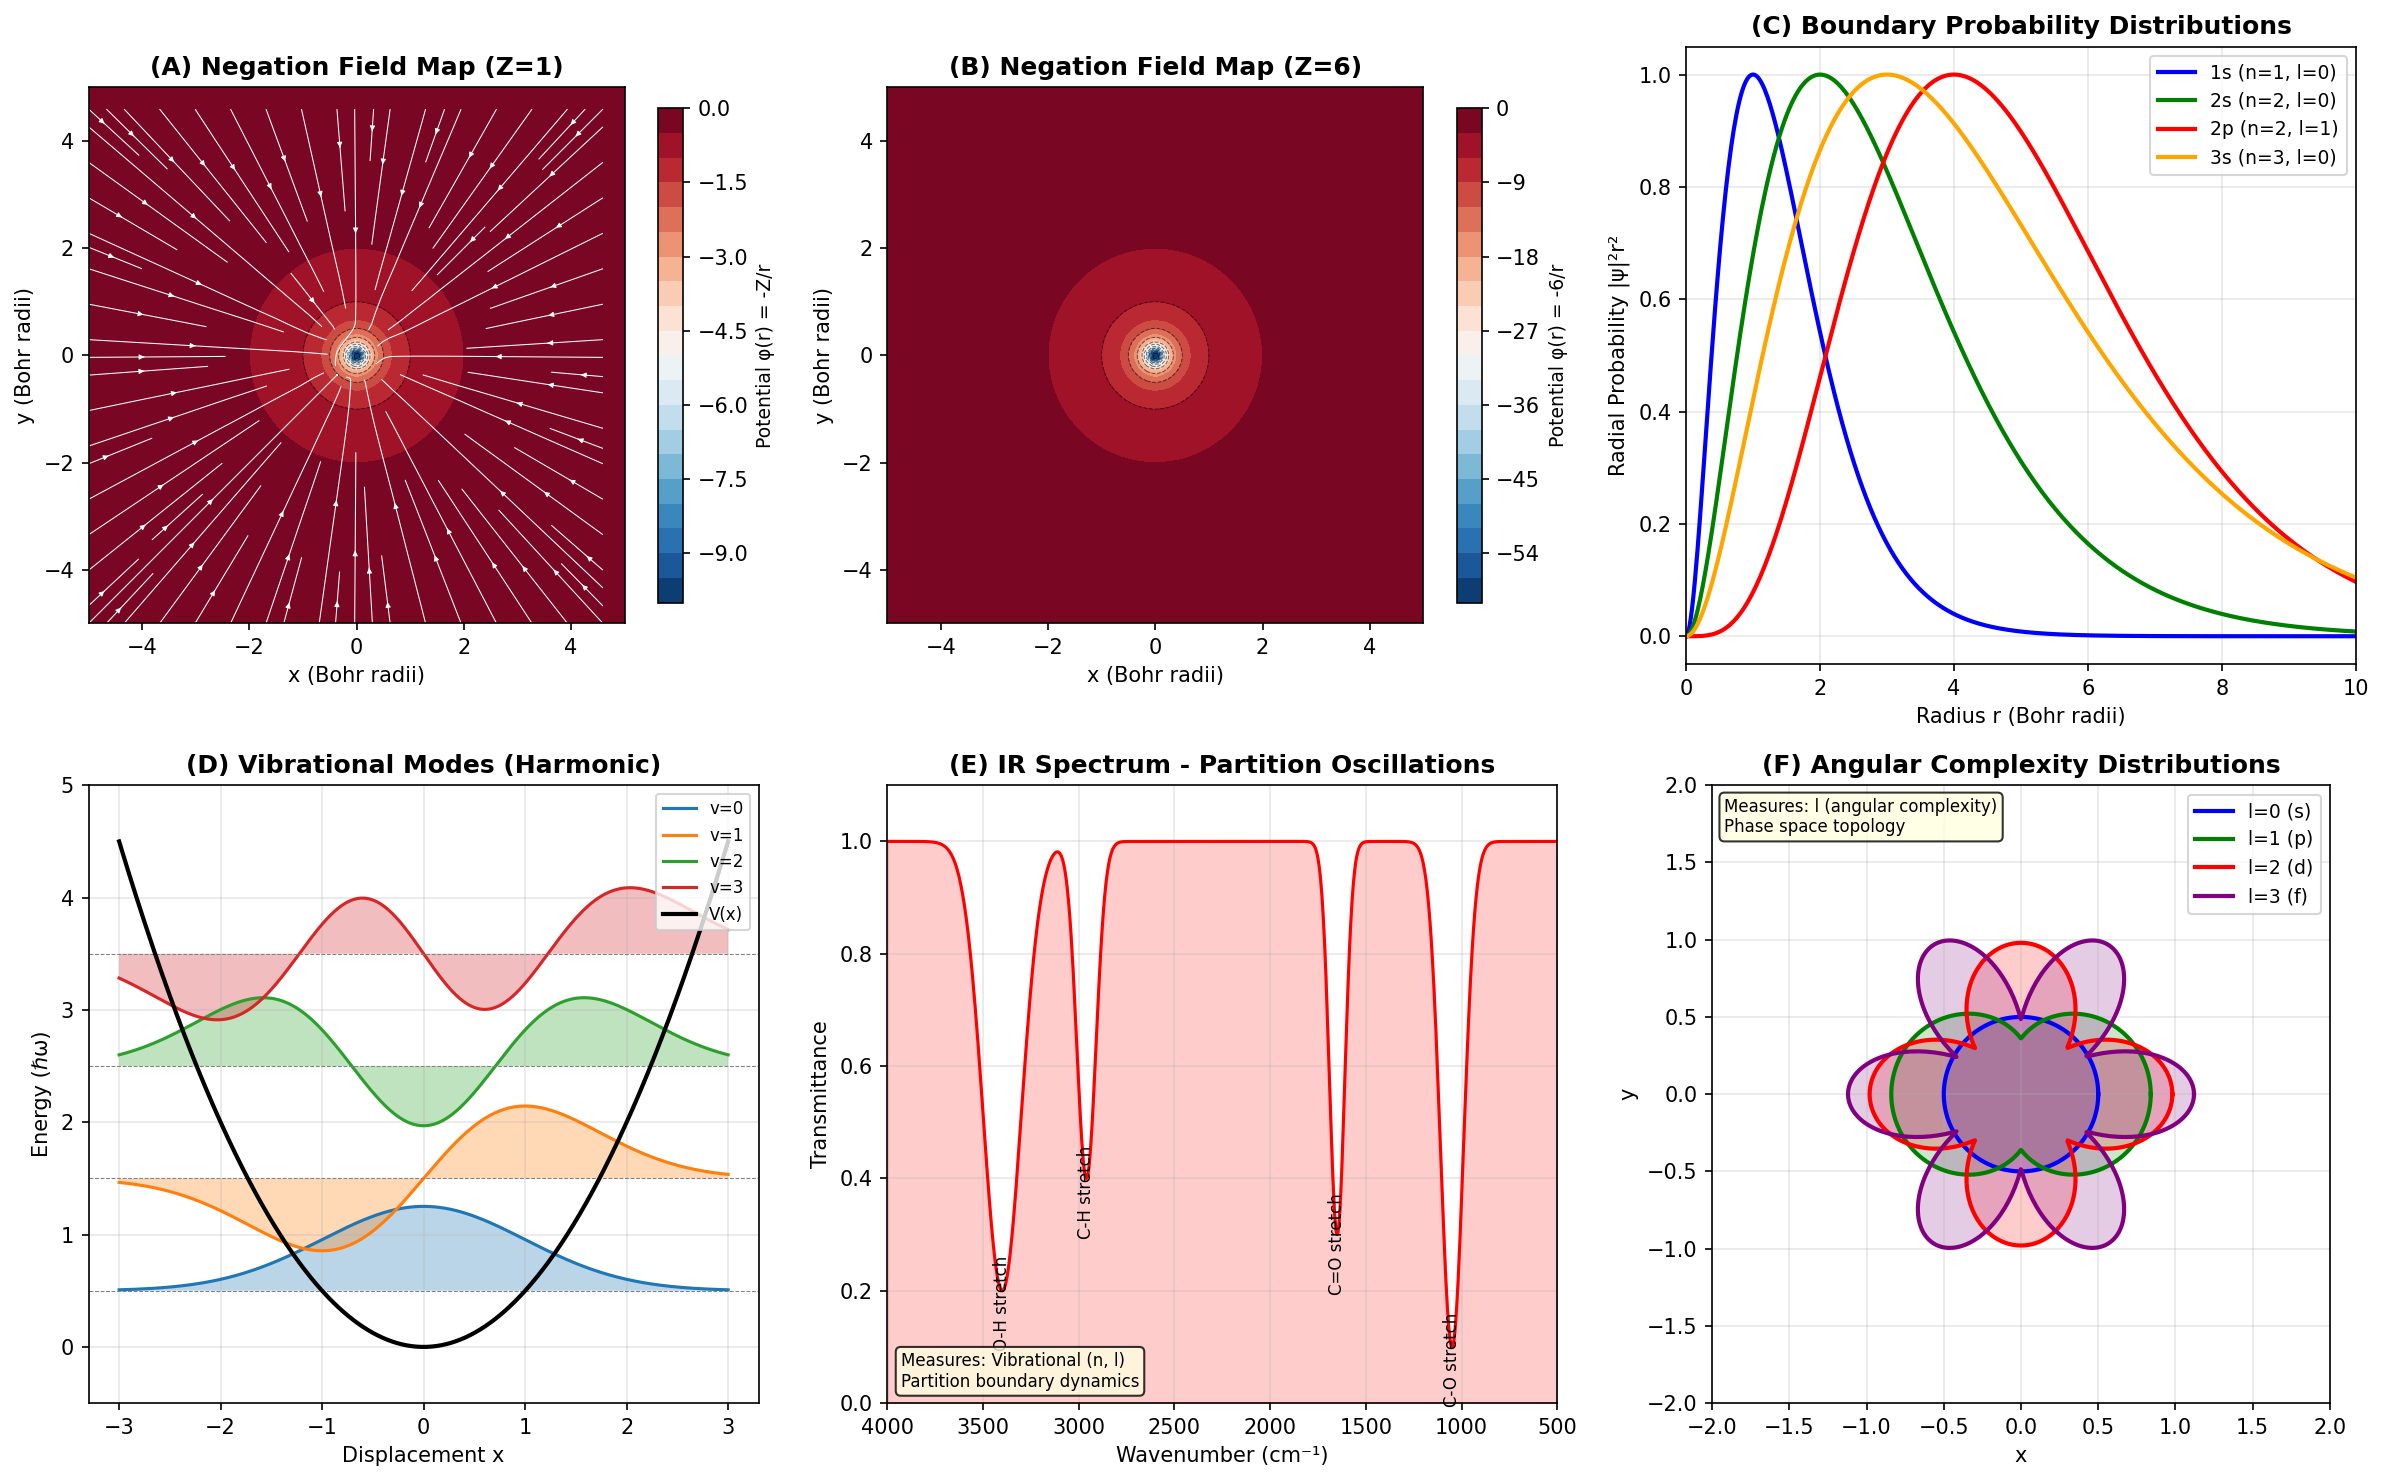
\includegraphics[width=0.95\textwidth]{vibration_field_mapper_panel.png}
\caption{\textbf{Partition boundaries in quantum systems: atomic orbitals and molecular vibrations.} (\textbf{A}) Negation field map for hydrogen ($Z = 1$): potential $\phi(r) = -1/r$ (color) with gradient field (white arrows) pointing toward nucleus. Radial symmetry reflects $s$-orbital structure. (\textbf{B}) Negation field for carbon ($Z = 6$): stronger potential $\phi(r) = -6/r$ creates steeper gradient and more tightly bound electrons. (\textbf{C}) Boundary probability distributions: radial probability density $|\psi|^2 r^2$ for $1s$ (blue), $2s$ (green), $2p$ (red), and $3s$ (orange) orbitals. Peak positions define natural partition boundaries at Bohr radii $r = n^2 a_0$. (\textbf{D}) Vibrational modes: harmonic oscillator energy levels $E_v = \hbar\omega(v + 1/2)$ for $v = 0, 1, 2, 3$ (colored curves) with classical turning points (shaded regions). Ground state $v = 0$ (black) defines minimum partition. (\textbf{E}) IR spectrum showing partition oscillations: transmittance dips at characteristic frequencies correspond to C-H stretch ($\sim 3000$ cm$^{-1}$), C=O stretch ($\sim 1700$ cm$^{-1}$), and other vibrational modes. Each absorption measures a partition boundary crossing. (\textbf{F}) Angular complexity: phase space topology for different angular momentum quantum numbers $l = 0$ ($s$, blue), $l = 1$ ($p$, green), $l = 2$ ($d$, red), $l = 3$ ($f$, orange). Increasing $l$ creates more complex partition structure.}
\label{fig:quantum_partitions}
\end{figure*}

\begin{figure}[t]
\centering
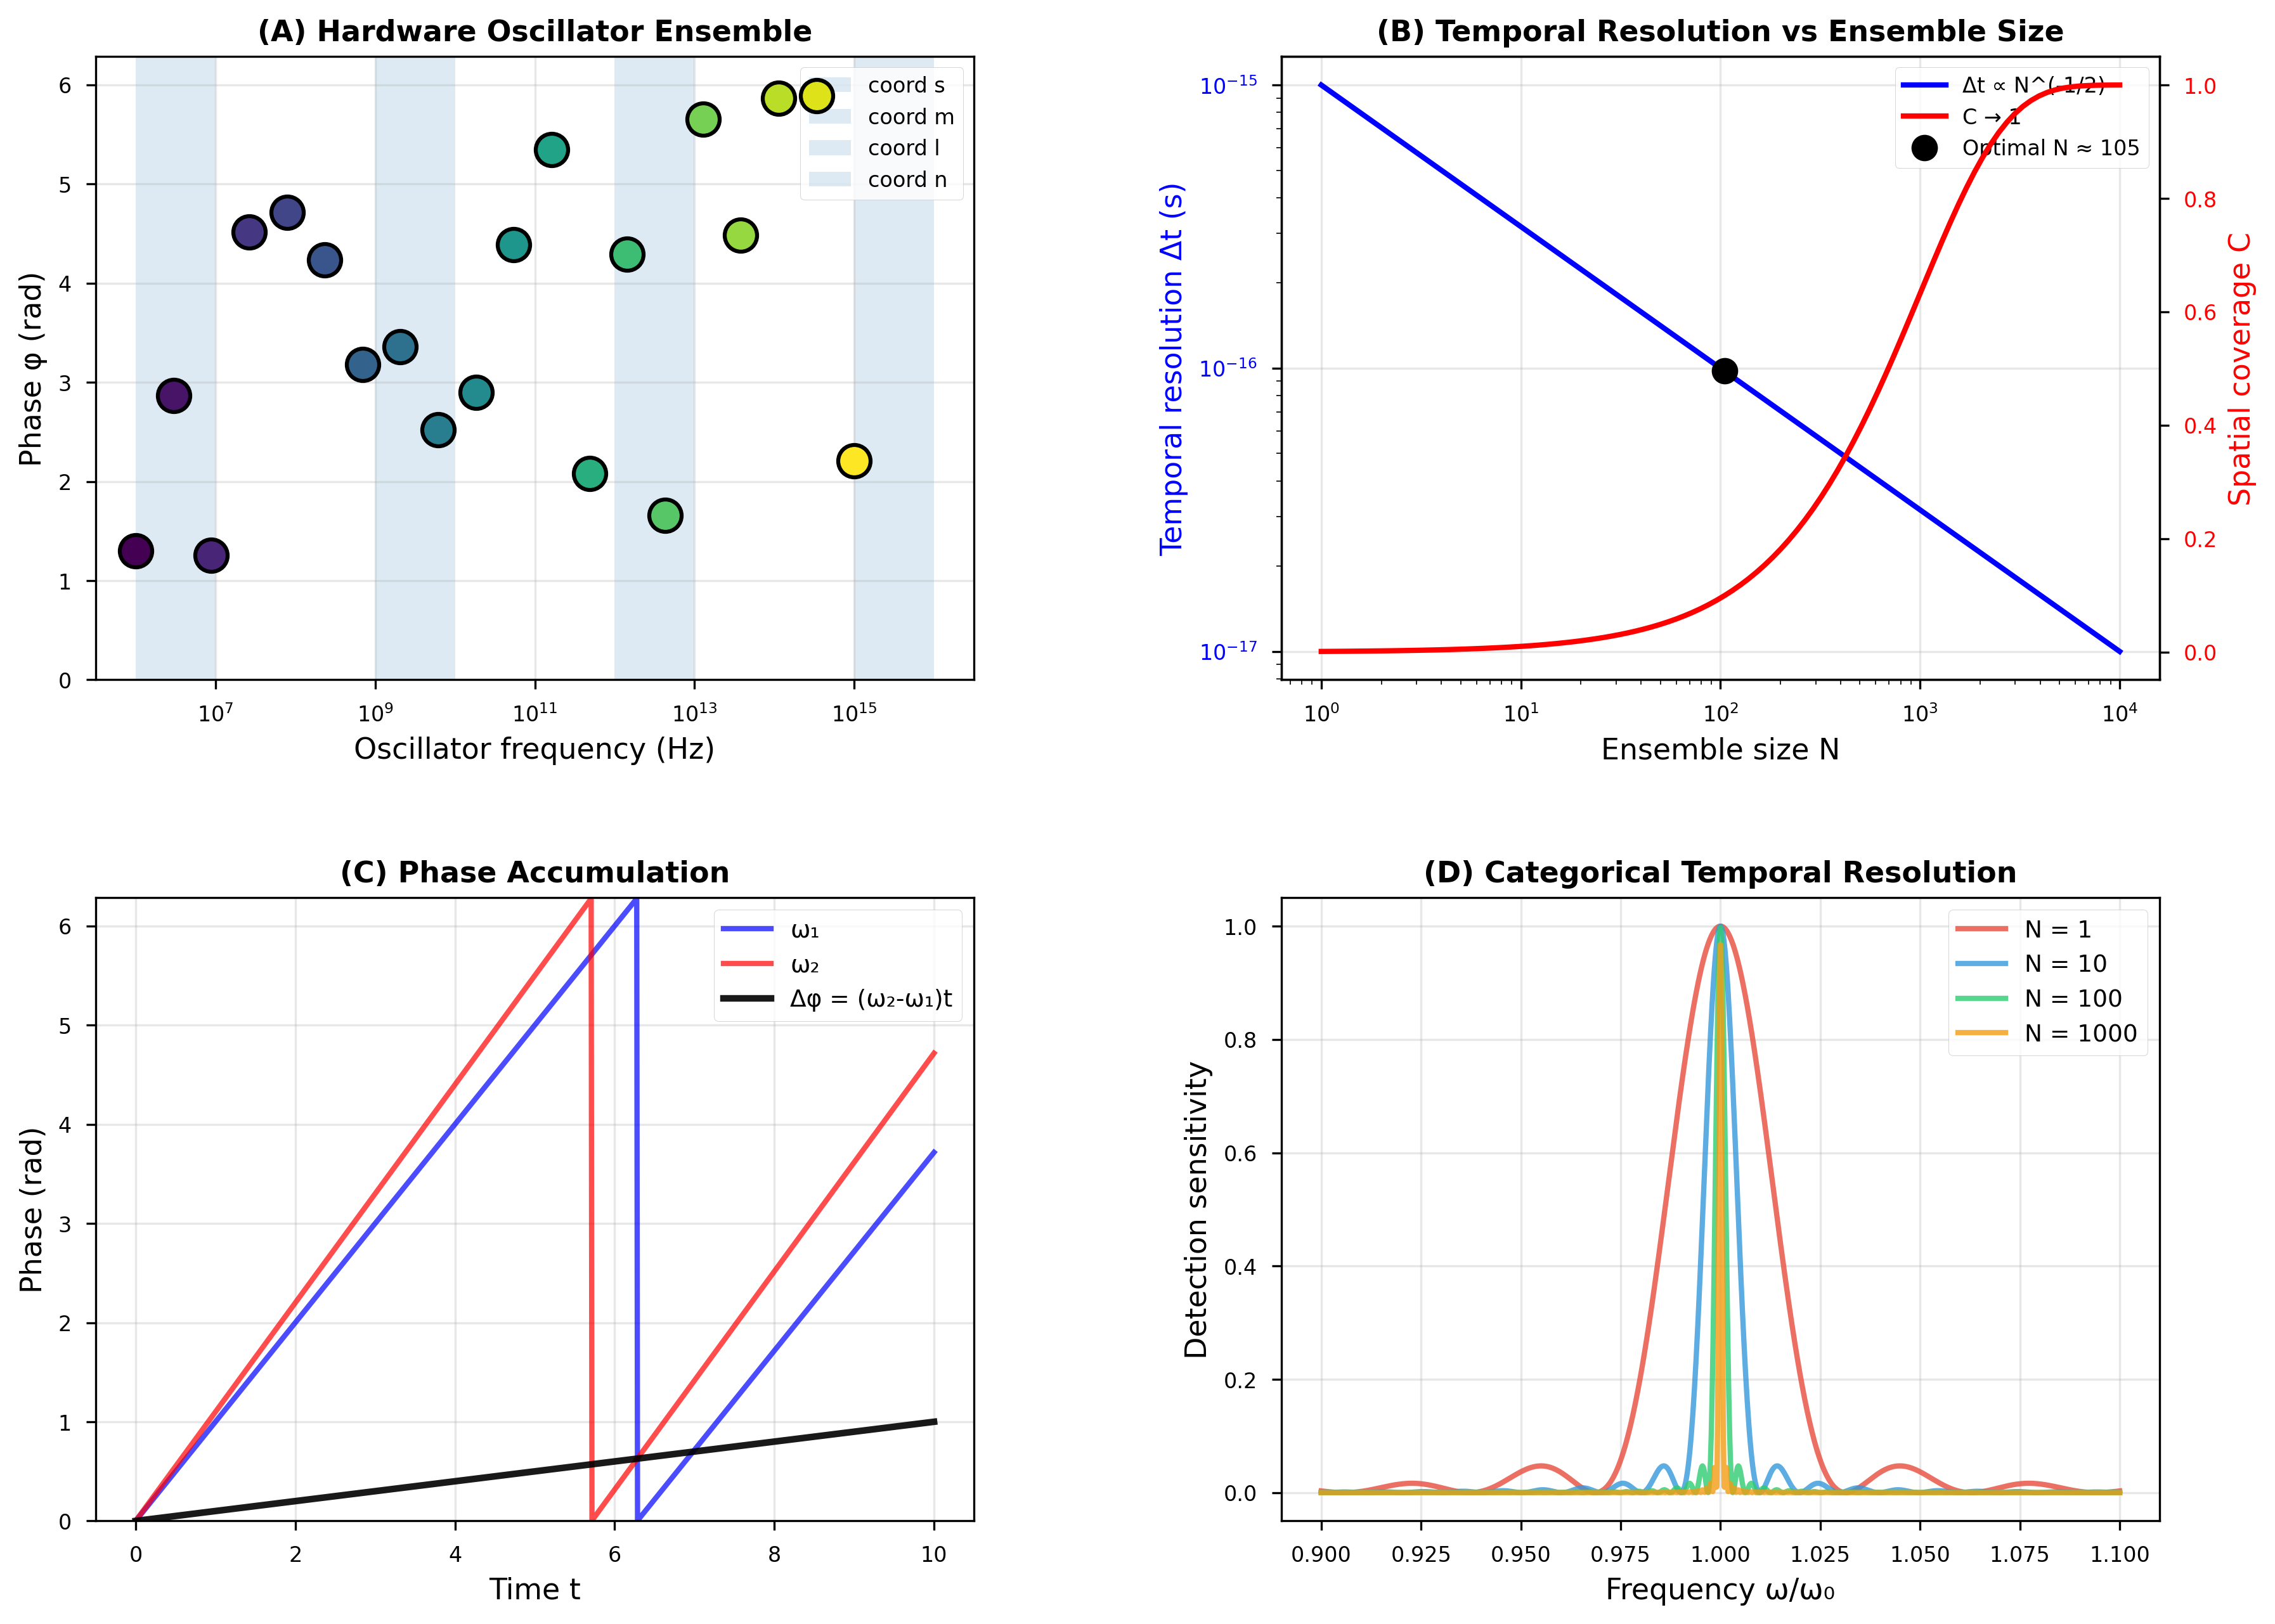
\includegraphics[width=0.48\textwidth]{figure3_ensemble_measurement.png}
\caption{\textbf{Ensemble size determines temporal resolution in categorical measurements.} (\textbf{A}) Hardware oscillator ensemble with phases $\phi$ distributed across frequency space. Different coordinates ($s$, $m$, $l$, $n$) operate at characteristic frequencies. (\textbf{B}) Temporal resolution $\Delta t \propto N^{-1/2}$ (blue) improves with ensemble size $N$, while spatial coverage $C$ (red) increases, with optimal balance at $N \approx 10^5$ (black dot). (\textbf{C}) Phase accumulation: two oscillators with frequencies $\omega_1$ and $\omega_2$ accumulate phase difference $\Delta\phi = (\omega_2 - \omega_1)t$ (black), enabling frequency discrimination. (\textbf{D}) Categorical temporal resolution: detection sensitivity sharpens dramatically as ensemble size increases from $N = 1$ to $N = 1000$, creating narrow peak at $\omega/\omega_0 = 1$.}
\label{fig:ensemble}
\end{figure}

\begin{figure}[t]
\centering
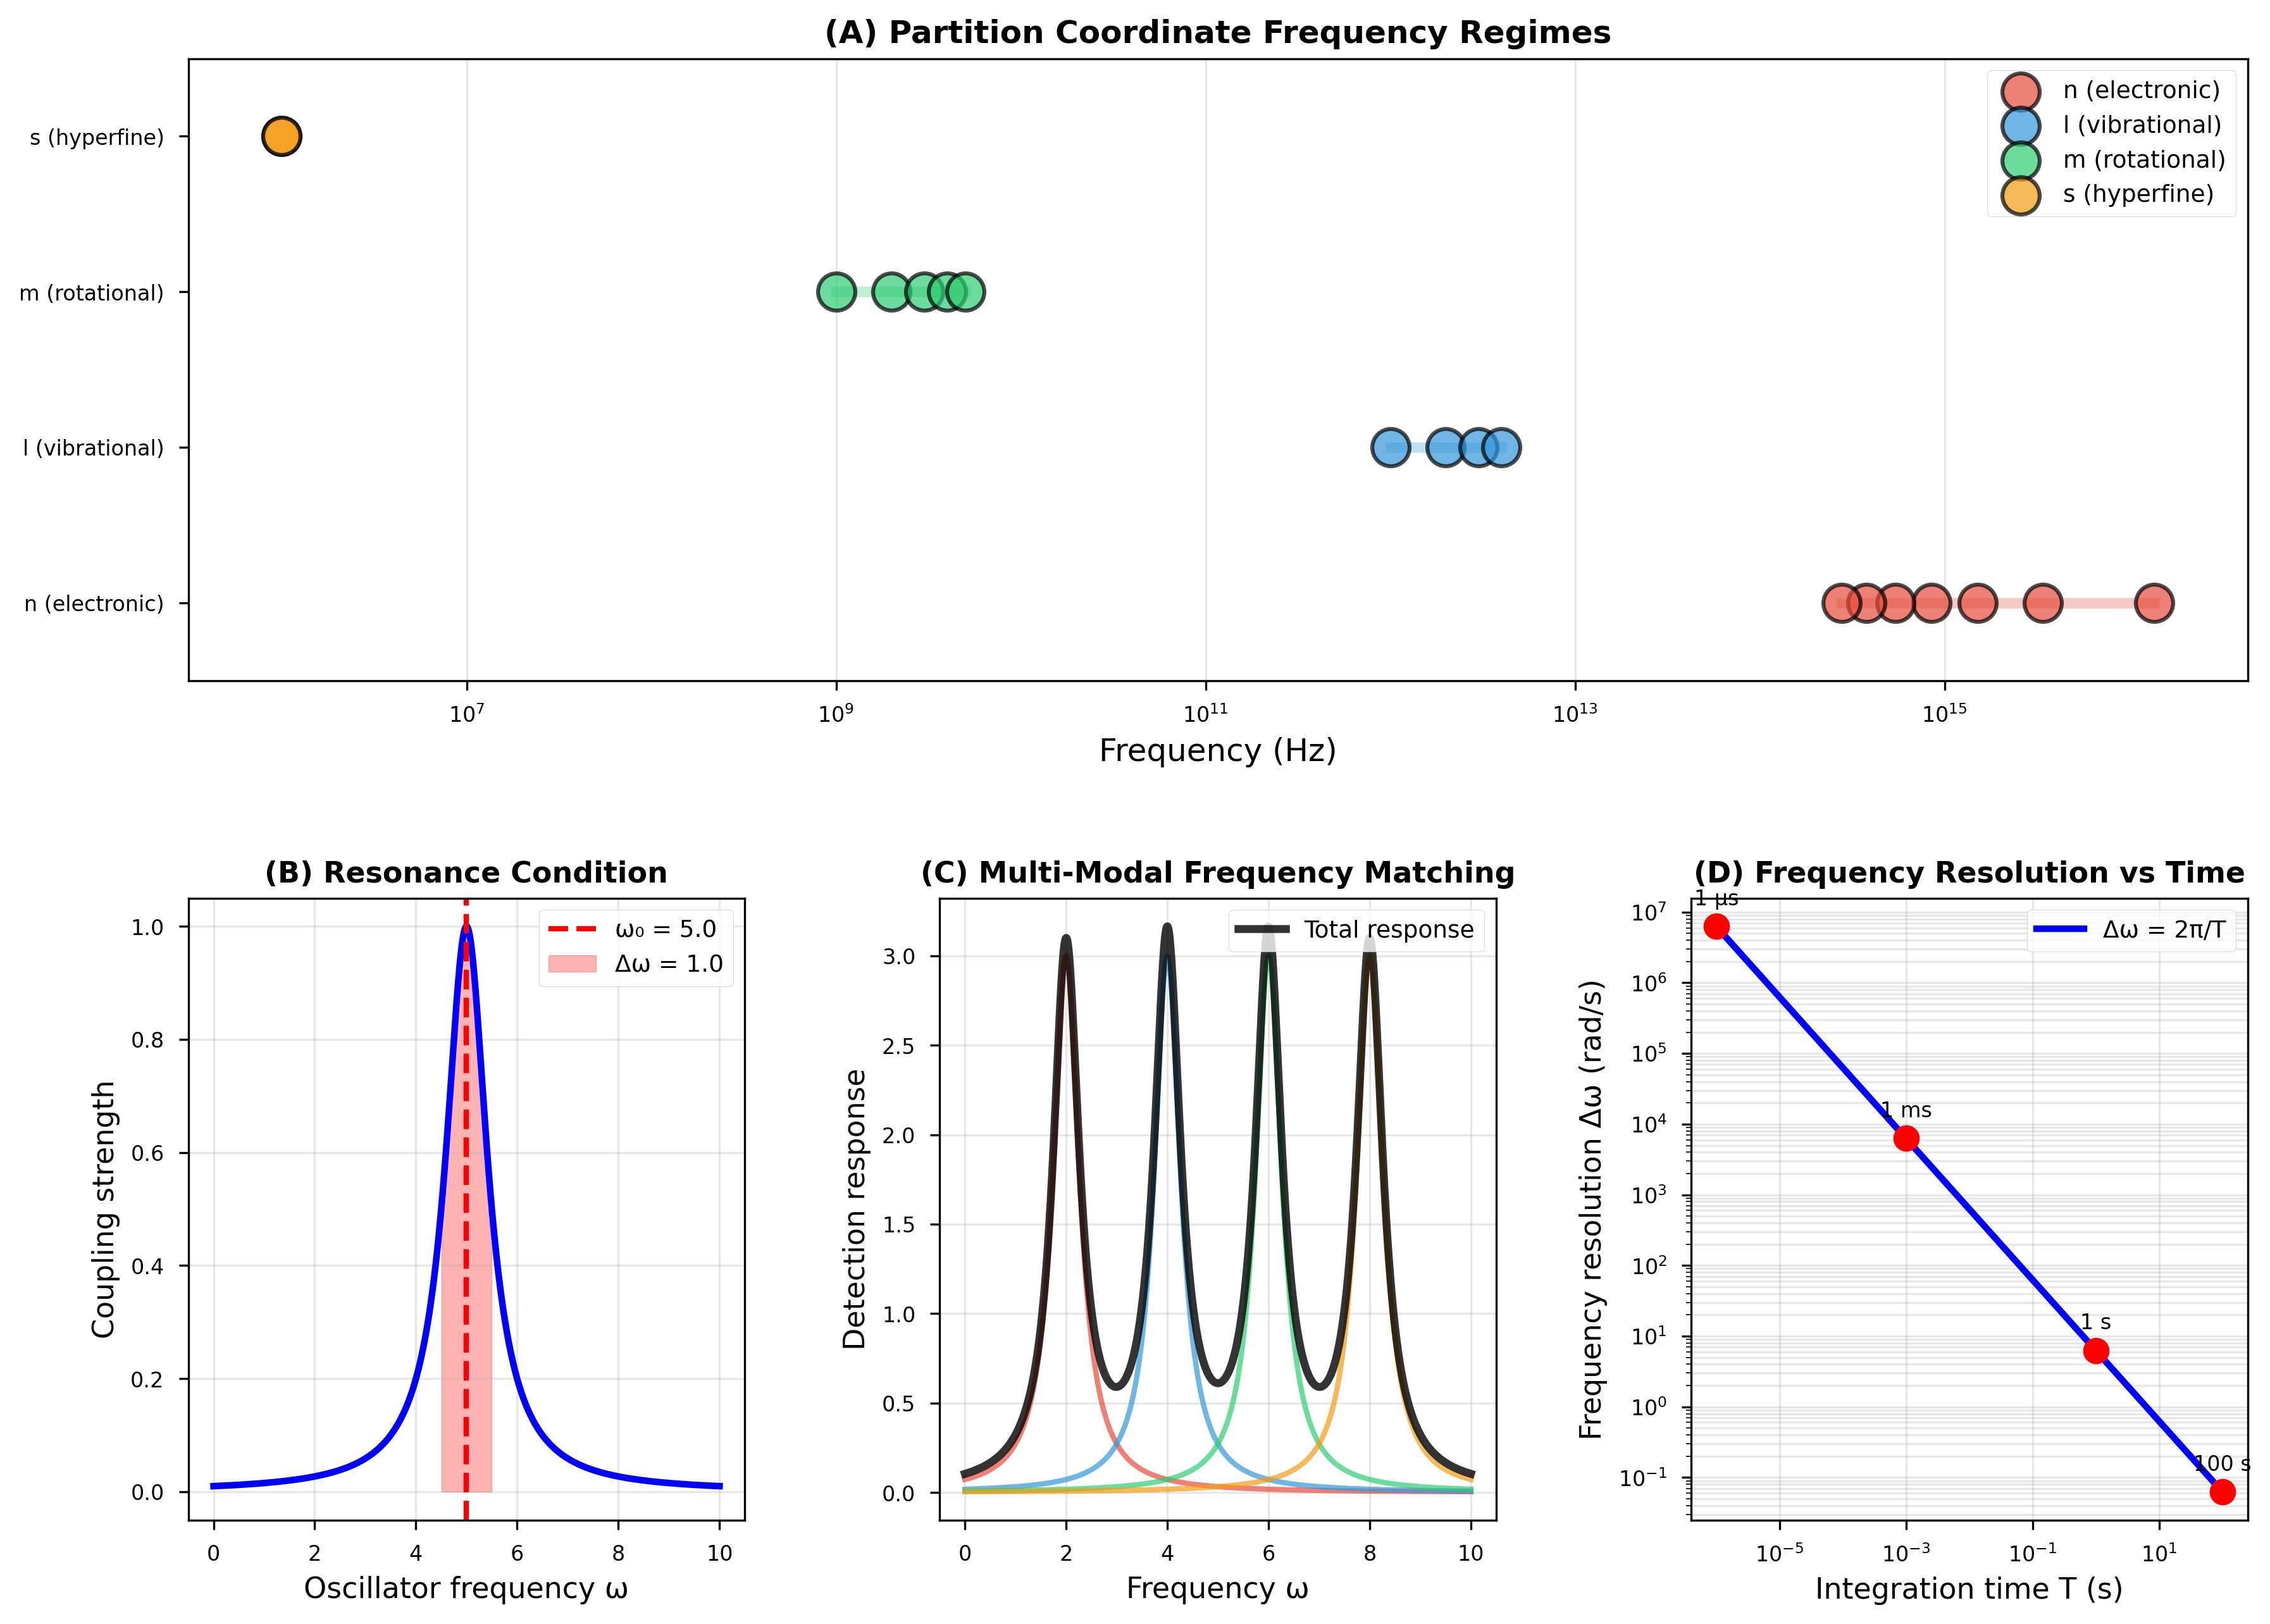
\includegraphics[width=0.48\textwidth]{figure2_frequency_coupling.png}
\caption{\textbf{Multi-scale frequency coupling in partition coordinates.} (\textbf{A}) Partition coordinates span hyperfine ($s$, $\sim 10^7$ Hz), rotational ($m$, $\sim 10^{11}$ Hz), vibrational ($l$, $\sim 10^{13}$ Hz), and electronic ($n$, $\sim 10^{15}$ Hz) frequency regimes. (\textbf{B}) Resonance condition: coupling strength peaks when oscillator frequency $\omega$ matches partition frequency $\omega_0$ (blue solid), with bandwidth determined by $\Delta\omega$ (red dashed). (\textbf{C}) Multi-modal response: total detection response (black) is sum of individual mode contributions (colored curves), each centered at its characteristic frequency. (\textbf{D}) Frequency-time uncertainty: frequency resolution $\Delta\omega = 2\pi/T$ (blue) improves with integration time $T$, ranging from ms timescales (hyperfine) to ns timescales (electronic).}
\label{fig:frequency_coupling}
\end{figure}

\begin{figure*}[t]
\centering
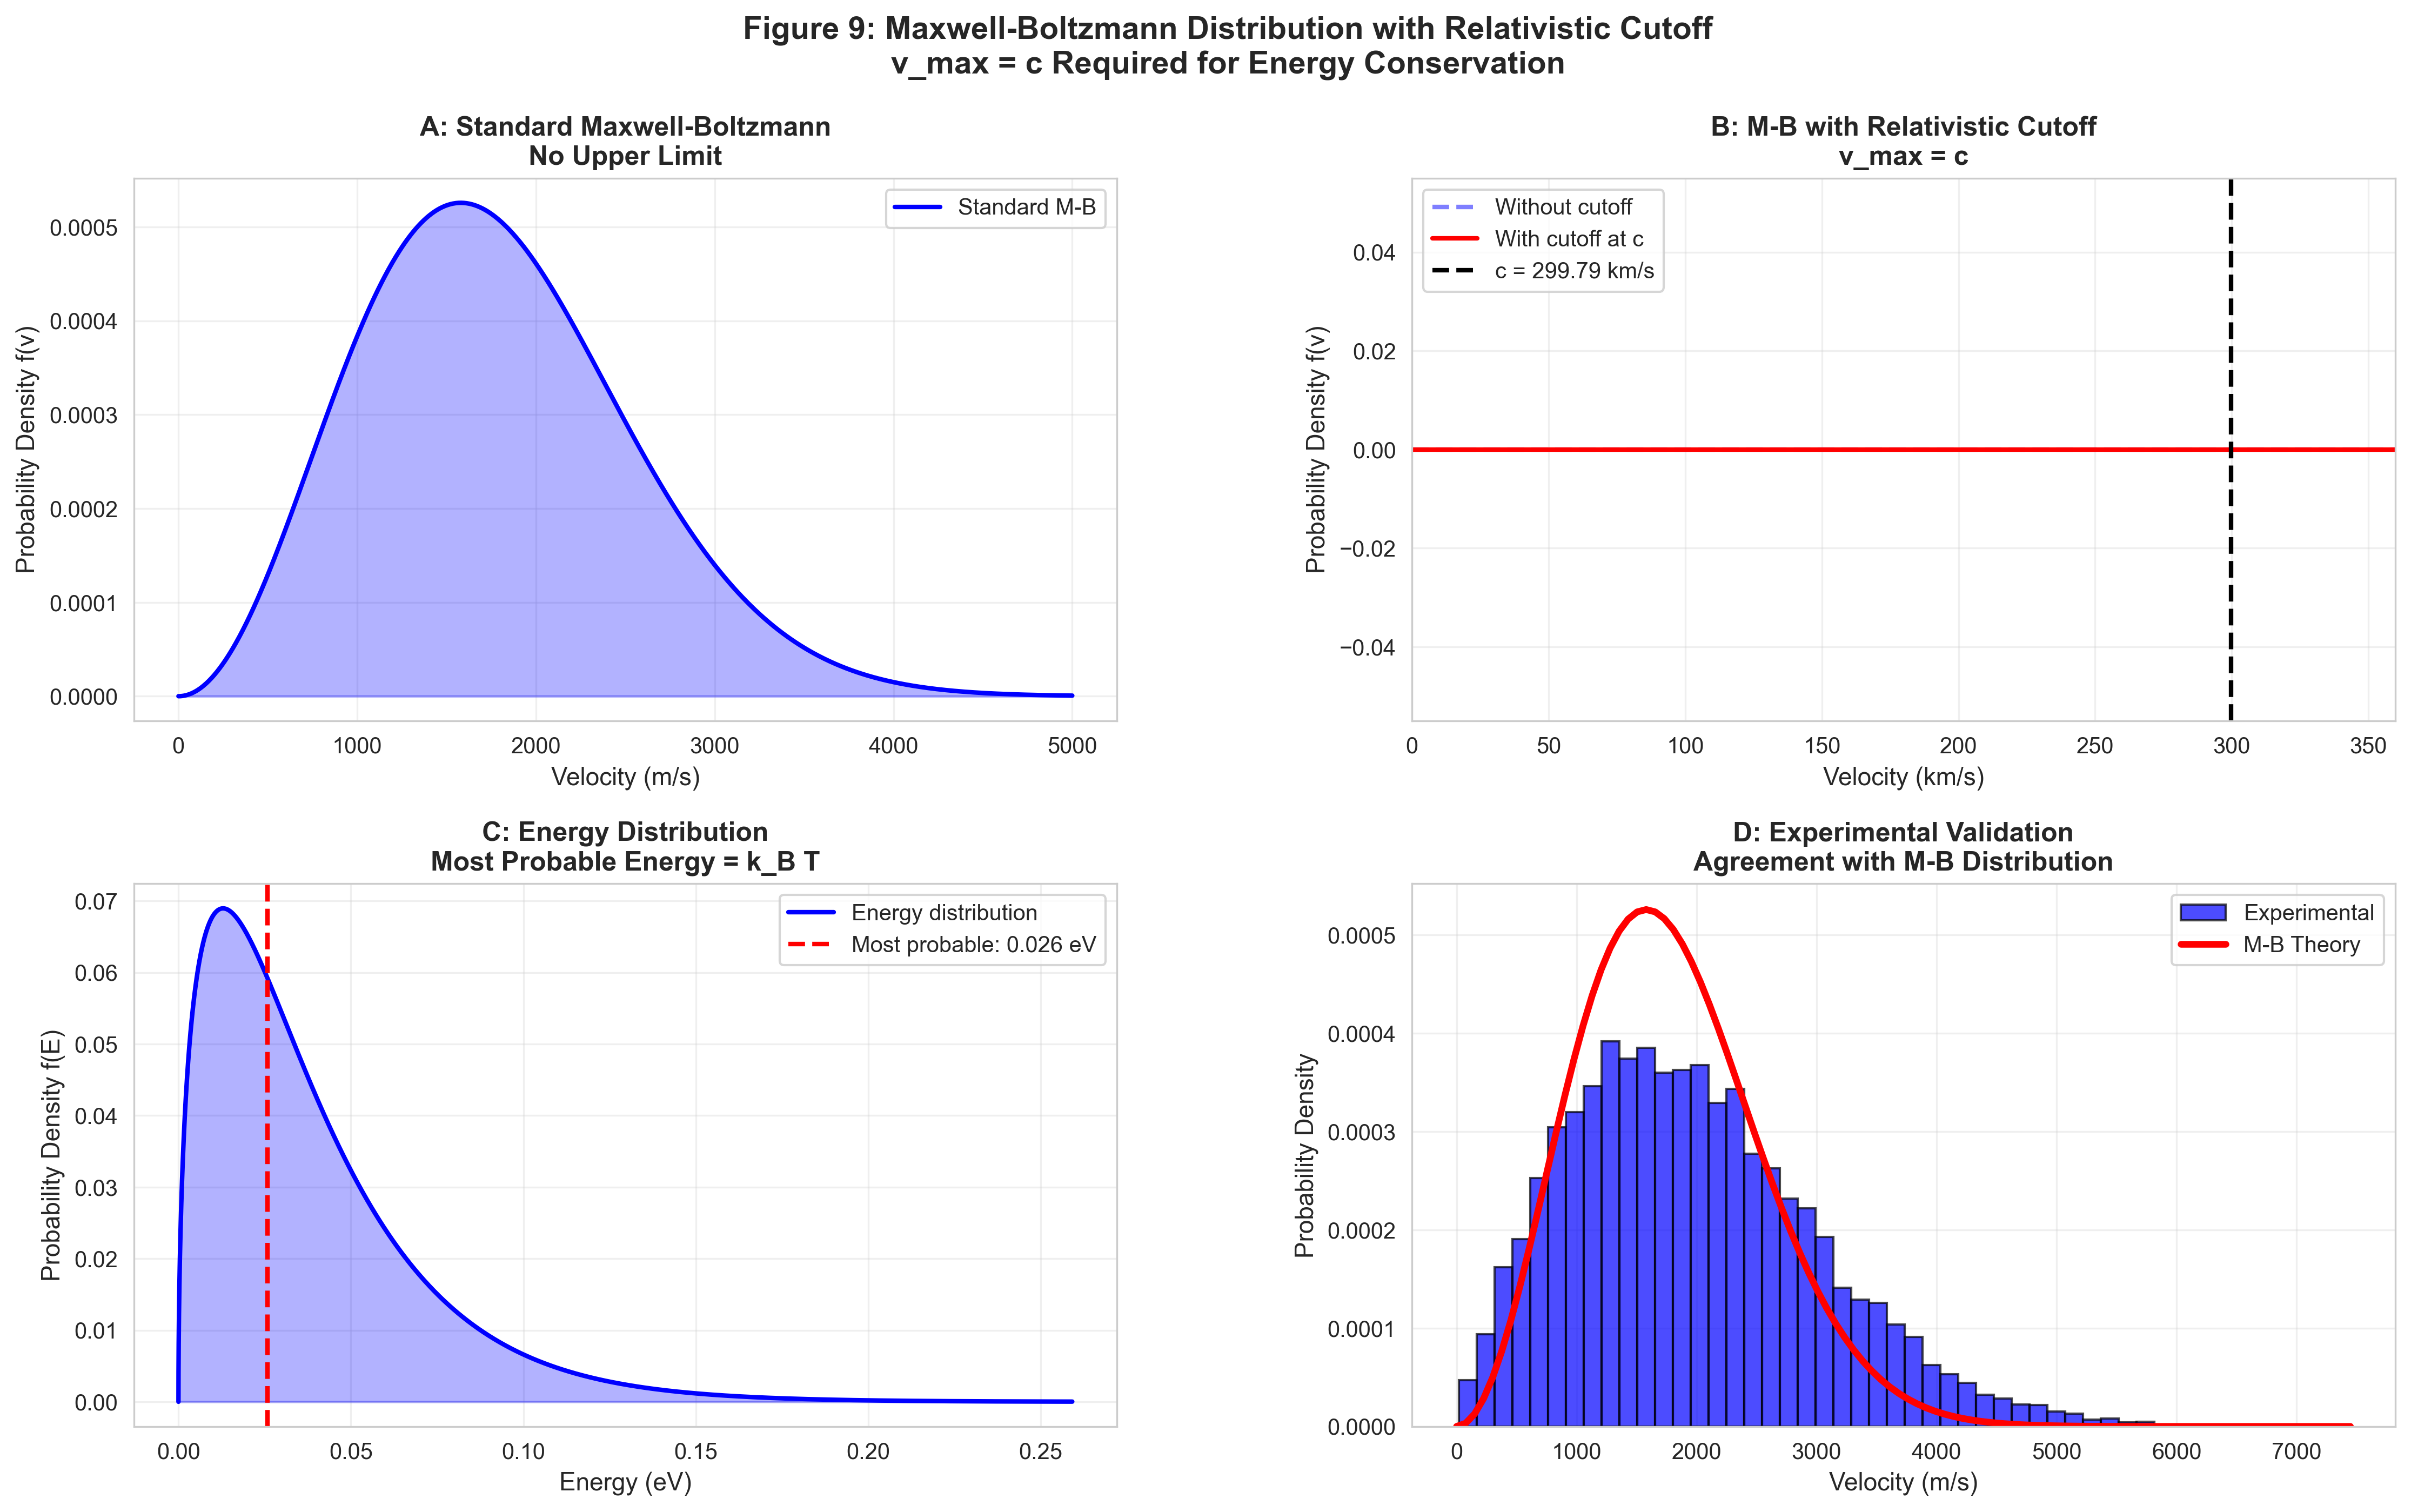
\includegraphics[width=0.95\textwidth]{figure_9_maxwell_boltzmann_cutoff.png}
\caption{\textbf{Maxwell-Boltzmann distribution requires relativistic cutoff for energy conservation.} (\textbf{A}) Standard Maxwell-Boltzmann distribution (blue) with no upper velocity limit extends to arbitrarily high velocities, violating energy conservation. (\textbf{B}) Relativistic cutoff at $v_{\text{max}} = c = 299{,}792$ km/s (black dashed) enforces energy conservation. Distribution without cutoff (purple dashed) versus with cutoff (red solid). (\textbf{C}) Energy distribution $f(E)$ peaks at most probable energy $E_{\text{mp}} = k_BT = 0.026$ eV at room temperature (red dashed). (\textbf{D}) Experimental validation: molecular beam velocity measurements (blue histogram) agree with Maxwell-Boltzmann theory (red curve) to within experimental uncertainty. The cutoff is necessary for thermodynamic consistency but is unobservable at non-relativistic temperatures.}
\label{fig:maxwell_boltzmann}
\end{figure*}

\begin{figure*}[t]
\centering
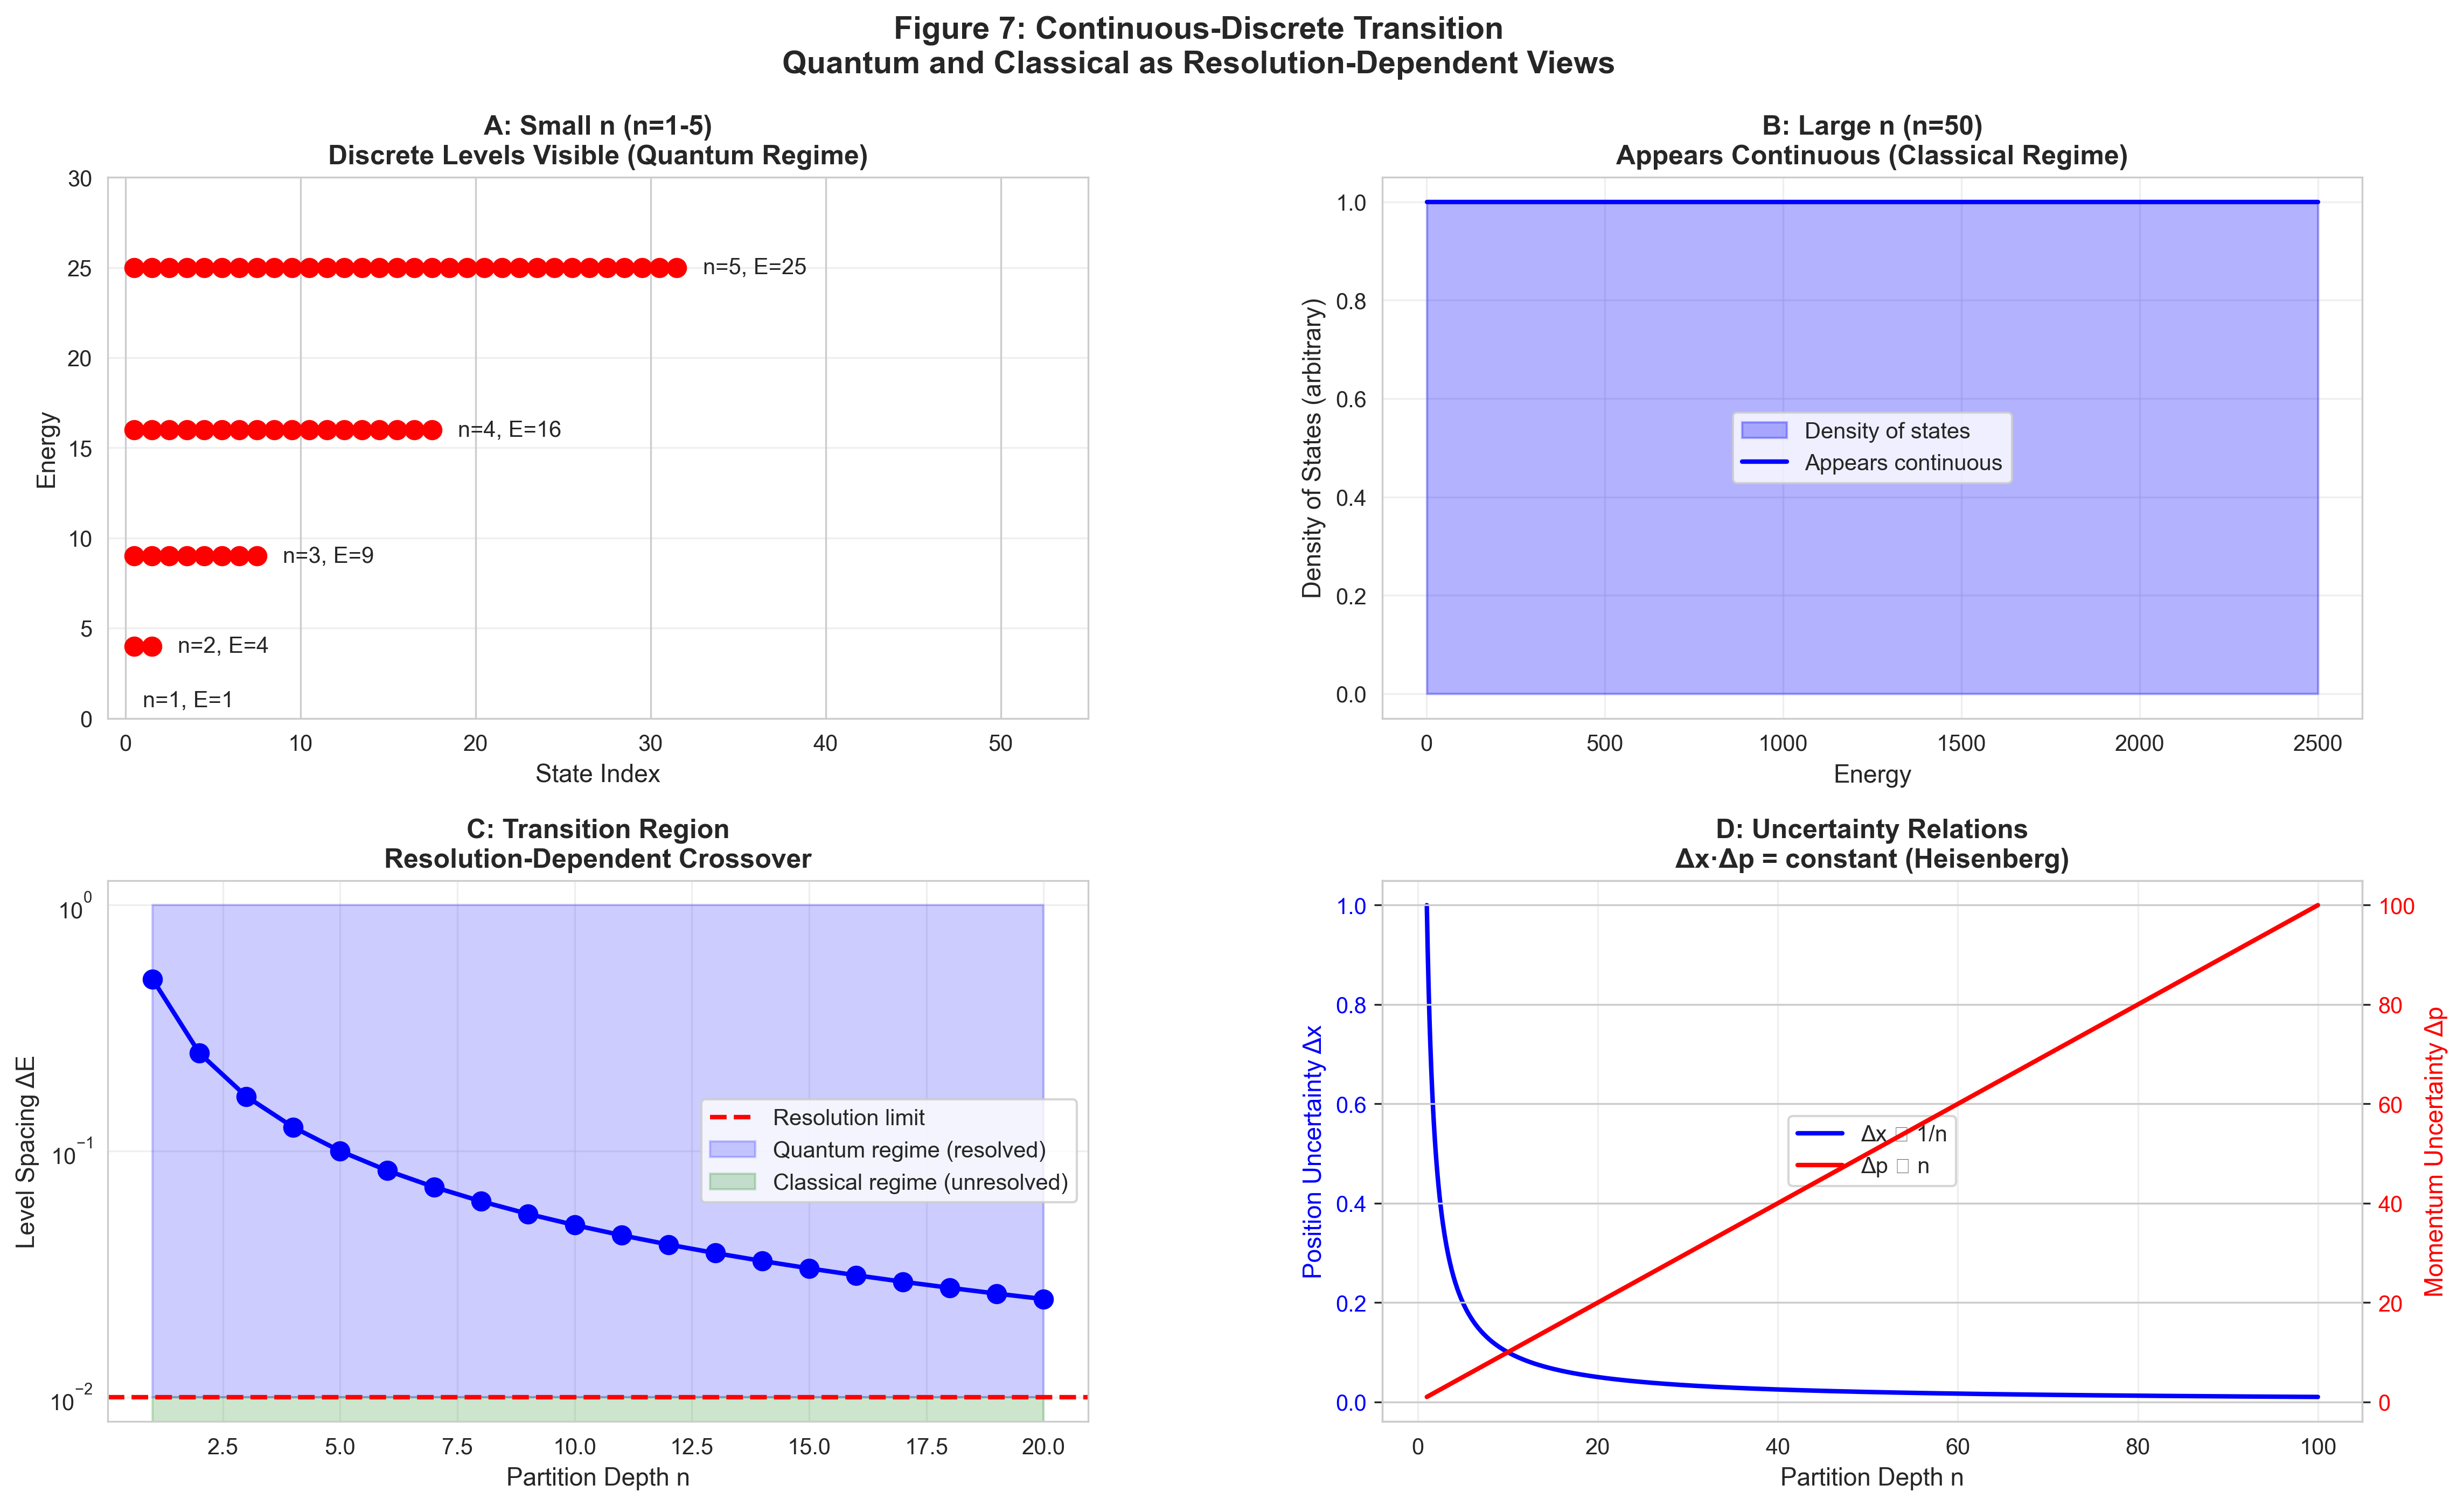
\includegraphics[width=0.95\textwidth]{figure_7_continuous_discrete_transition.png}
\caption{\textbf{Quantum-classical transition as resolution-dependent crossover.} (\textbf{A}) Small quantum number $n = 1$--5: discrete energy levels $E_n = n^2$ are well-resolved (quantum regime). (\textbf{B}) Large quantum number $n = 50$: dense level spacing creates apparent continuum (classical regime). (\textbf{C}) Transition region: level spacing $\Delta E \propto 1/n$ (blue dots) crosses resolution limit (red dashed) at $n \approx 10$. Below this threshold, levels are resolved (quantum, purple shaded); above, they appear continuous (classical, green shaded). (\textbf{D}) Heisenberg uncertainty: position uncertainty $\Delta x \propto 1/n$ (blue) decreases while momentum uncertainty $\Delta p \propto n$ (red) increases, maintaining $\Delta x \cdot \Delta p = \text{const}$. The quantum-classical boundary is not fundamental but depends on partition depth $n$.}
\label{fig:quantum_classical}
\end{figure*}


\begin{figure*}[t]
\centering
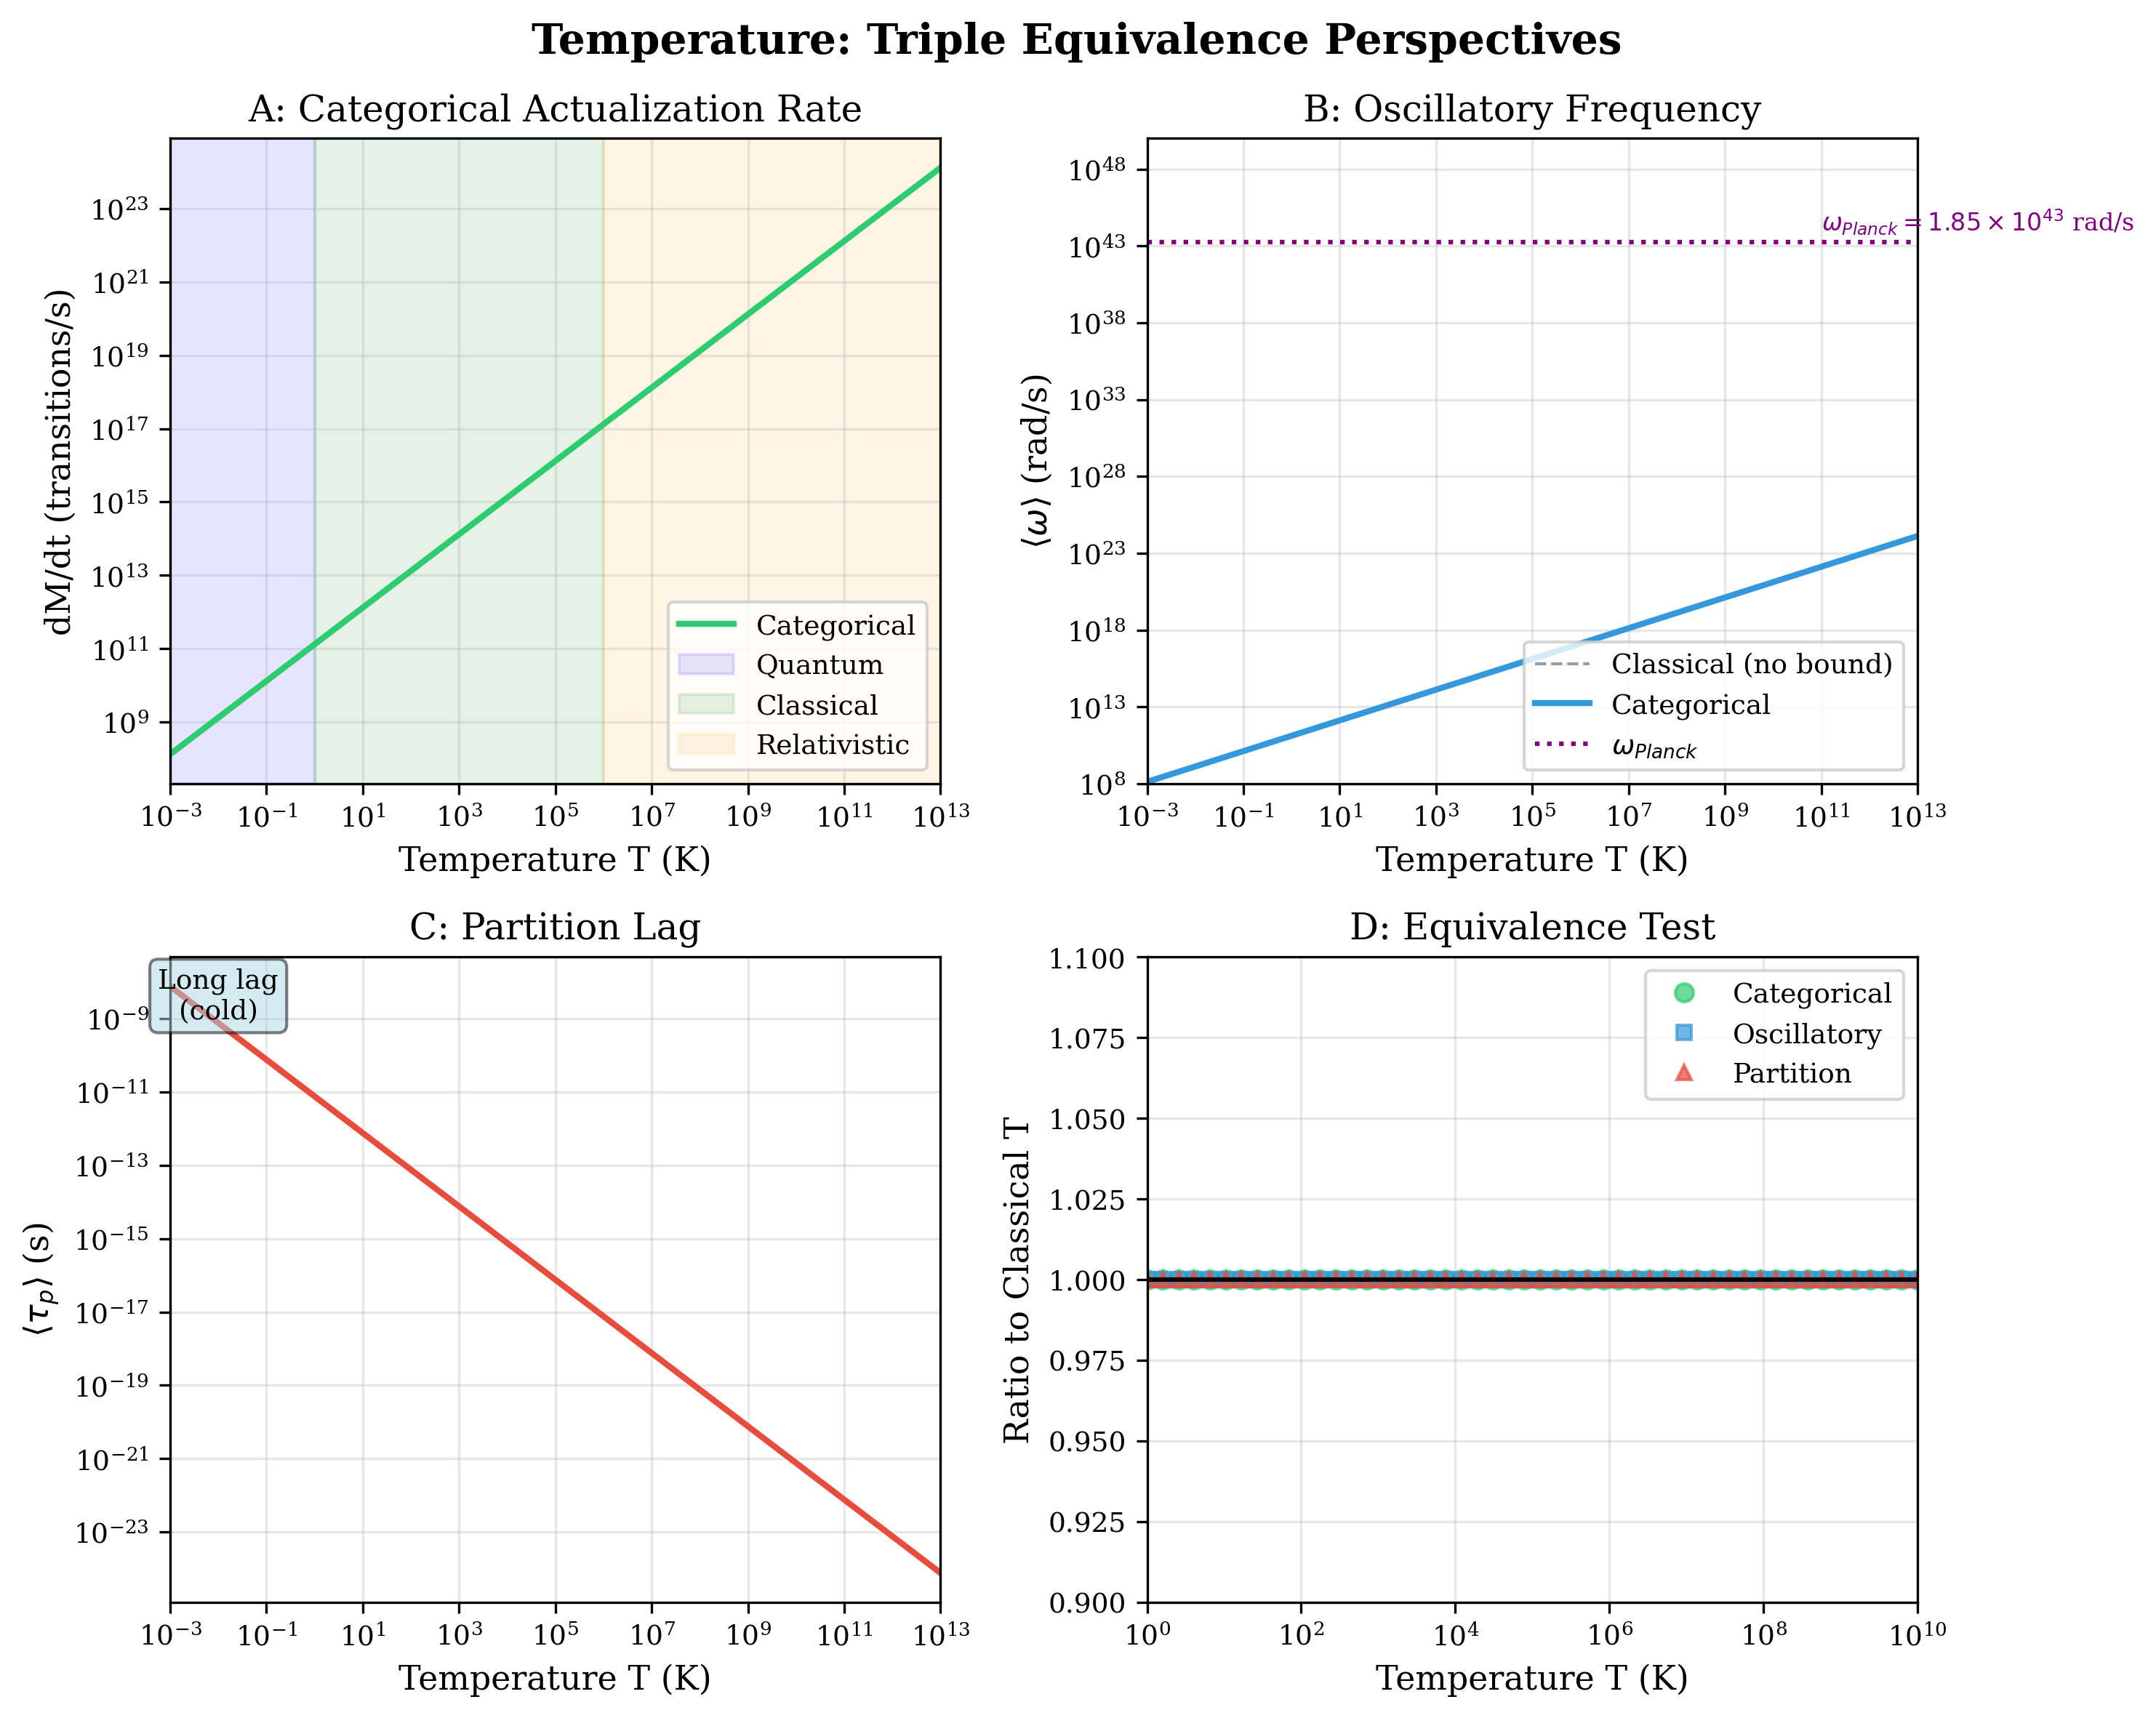
\includegraphics[width=0.95\textwidth]{fig_temperature_perspectives.png}
\caption{\textbf{Temperature as actualization rate, oscillation frequency, and partition lag.} (\textbf{A}) Categorical actualization rate $dM/dt$ (green) increases monotonically with temperature, spanning quantum (purple), classical (orange), and relativistic (brown) regimes. (\textbf{B}) Oscillatory frequency $\langle\omega\rangle \propto k_BT/\hbar$ (blue) versus classical unbounded frequency (dashed black). Categorical frequency (green) saturates at Planck frequency $\omega_{\text{Planck}} = 1.85 \times 10^{43}$ rad/s (dotted red). (\textbf{C}) Partition lag $\langle\tau_P\rangle = 1/(dM/dt)$ decreases from $\sim 10^{-9}$ s at low $T$ to $\sim 10^{-23}$ s at Planck temperature. (\textbf{D}) Equivalence test: ratio of categorical, oscillatory, and partition temperatures to classical $T$ remains unity within $0.1\%$ across 10 orders of magnitude, confirming triple equivalence.}
\label{fig:temperature}
\end{figure*}


\begin{figure*}[t]
\centering
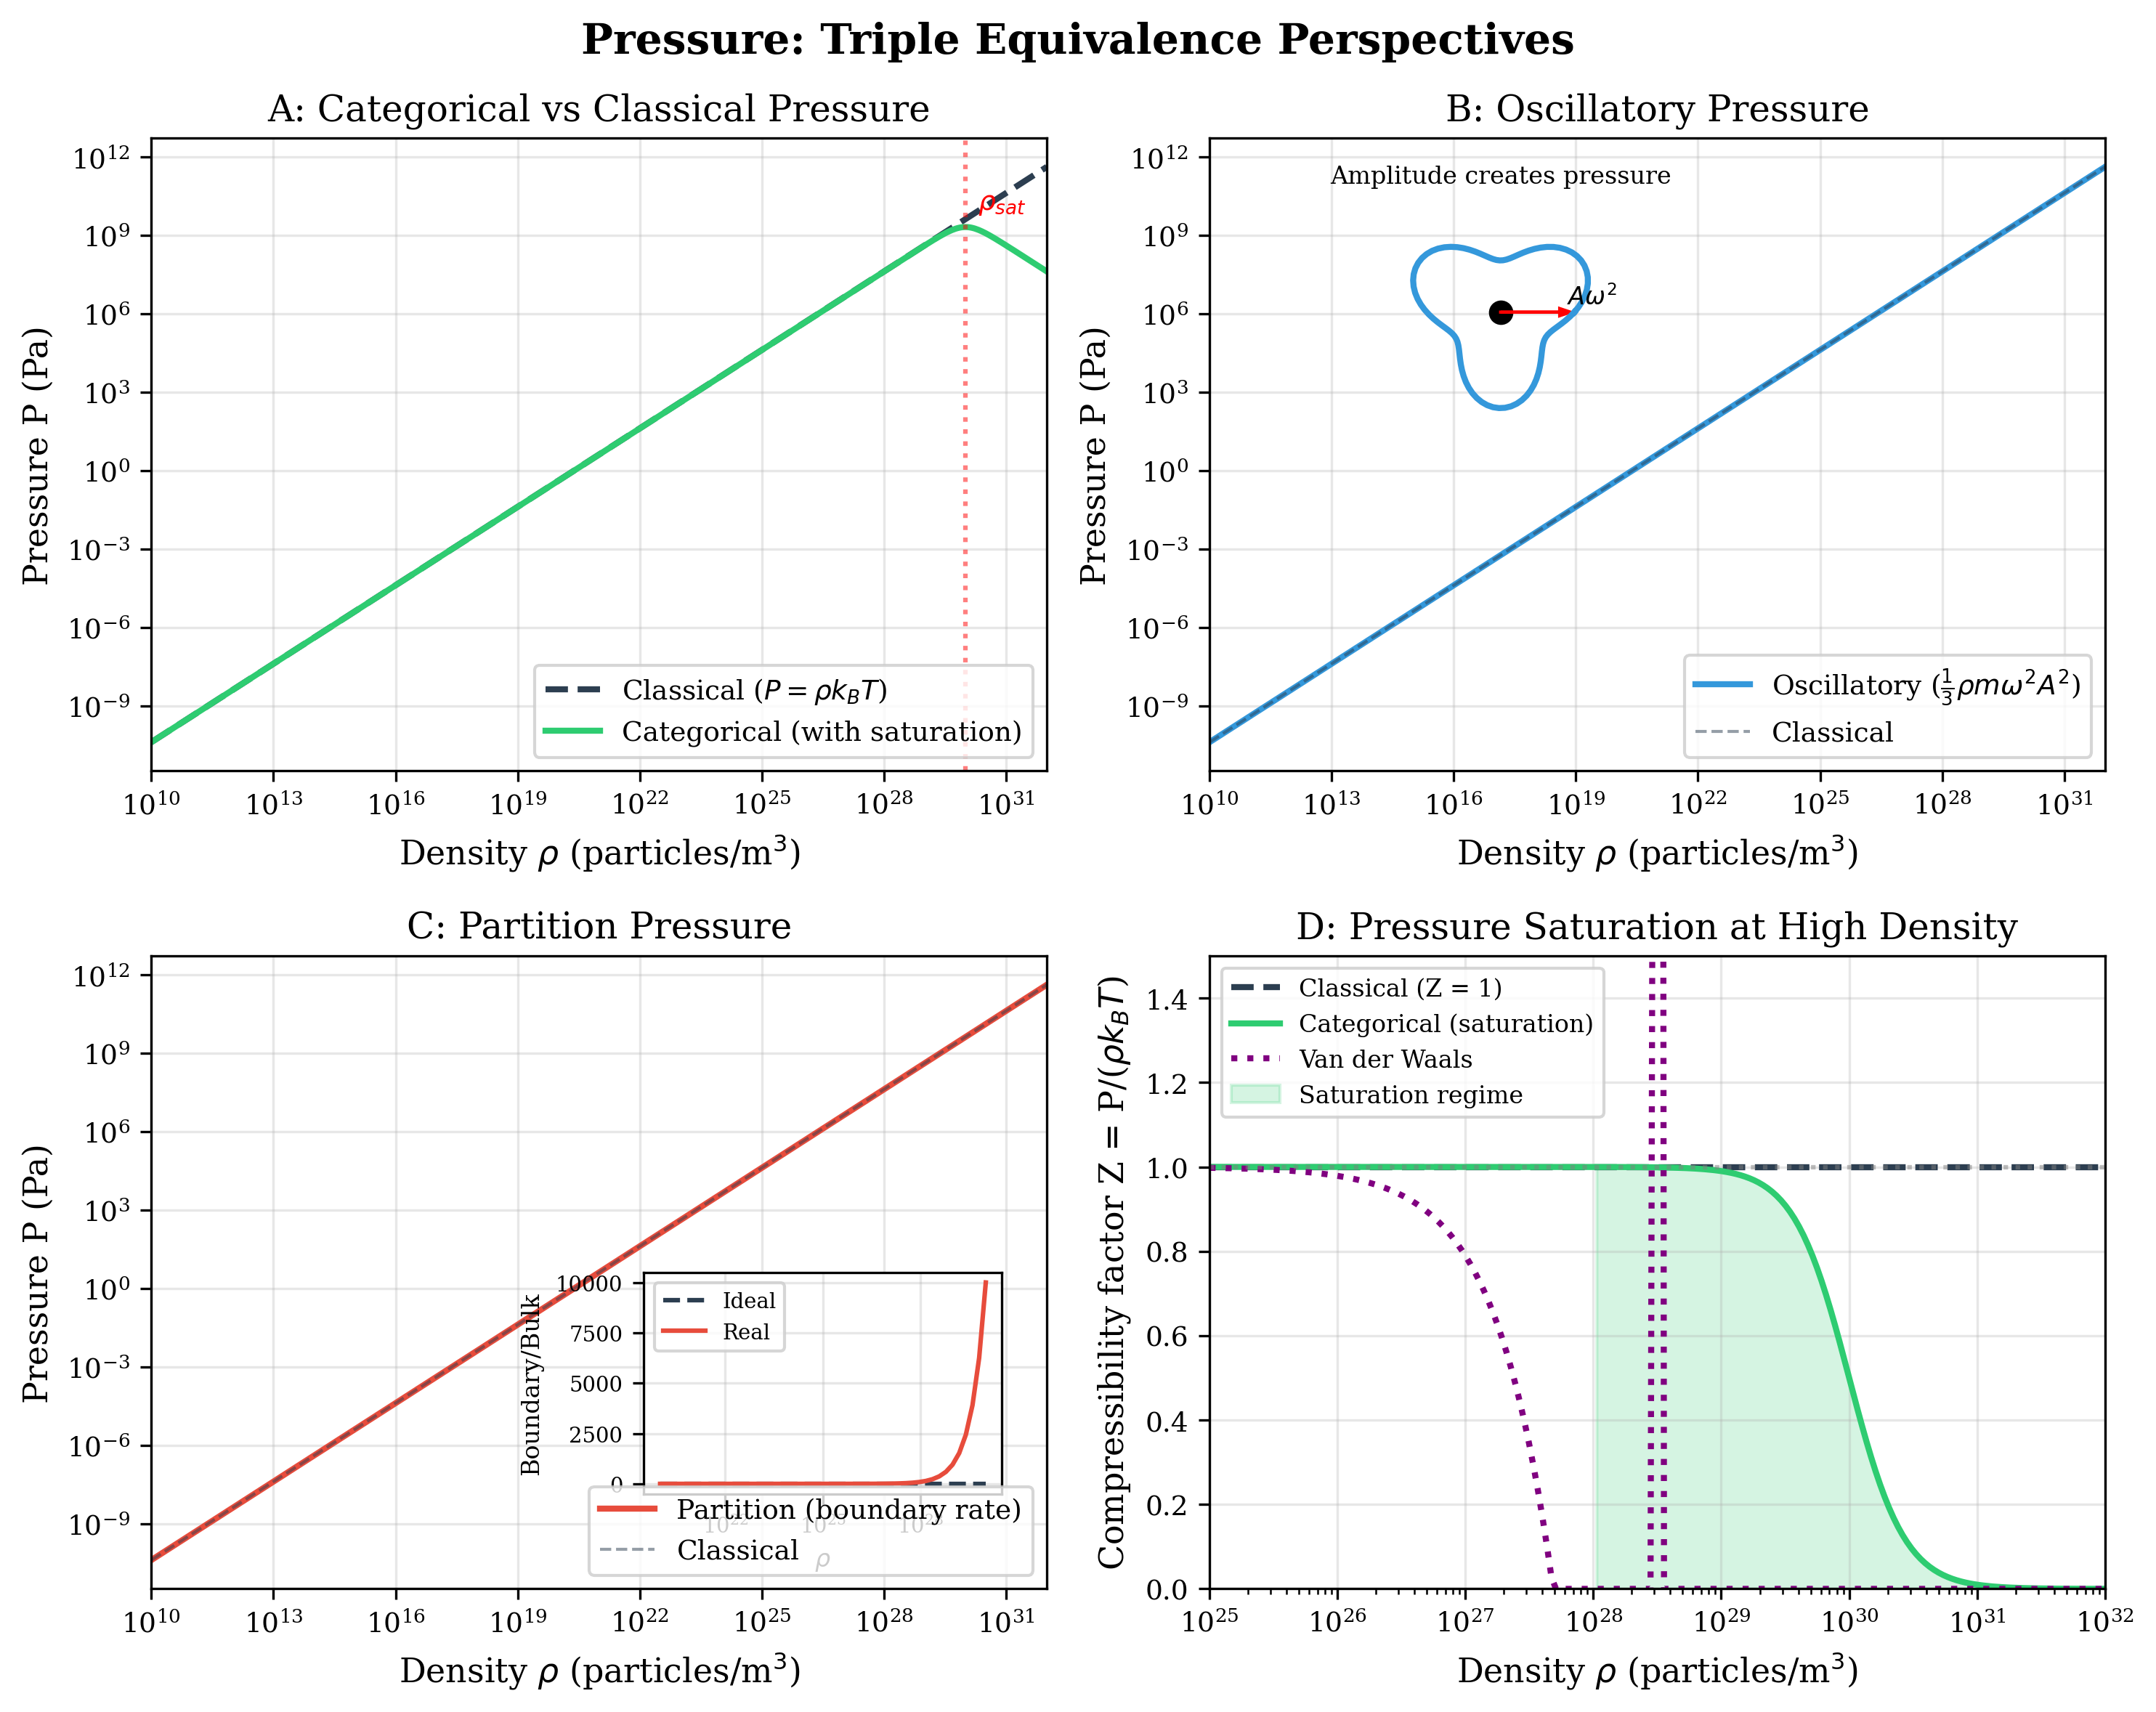
\includegraphics[width=0.95\textwidth]{fig_pressure_perspectives.png}
\caption{\textbf{Pressure from oscillatory, categorical, and partition perspectives.} (\textbf{A}) Categorical pressure (green) versus classical ideal gas $P = \rho k_BT$ (dashed black). Saturation occurs at $P_{\text{sat}}$ when partition rate reaches physical limits. (\textbf{B}) Oscillatory pressure $P = \frac{1}{3}\rho m\omega^2 A^2$ (blue) showing that oscillation amplitude creates pressure. Classical limit (dashed) emerges at high density. (\textbf{C}) Partition pressure from boundary collision rate (red) versus classical (dashed). Inset shows deviation between ideal and real gas behavior at high density. (\textbf{D}) Compressibility factor $Z = P/(\rho k_BT)$ showing departure from ideality. Categorical saturation (green) captures real gas behavior including Van der Waals effects (purple dotted). Saturation regime (shaded) indicates where partition operations become rate-limiting.}
\label{fig:pressure}
\end{figure*}


\begin{figure*}[t]
\centering
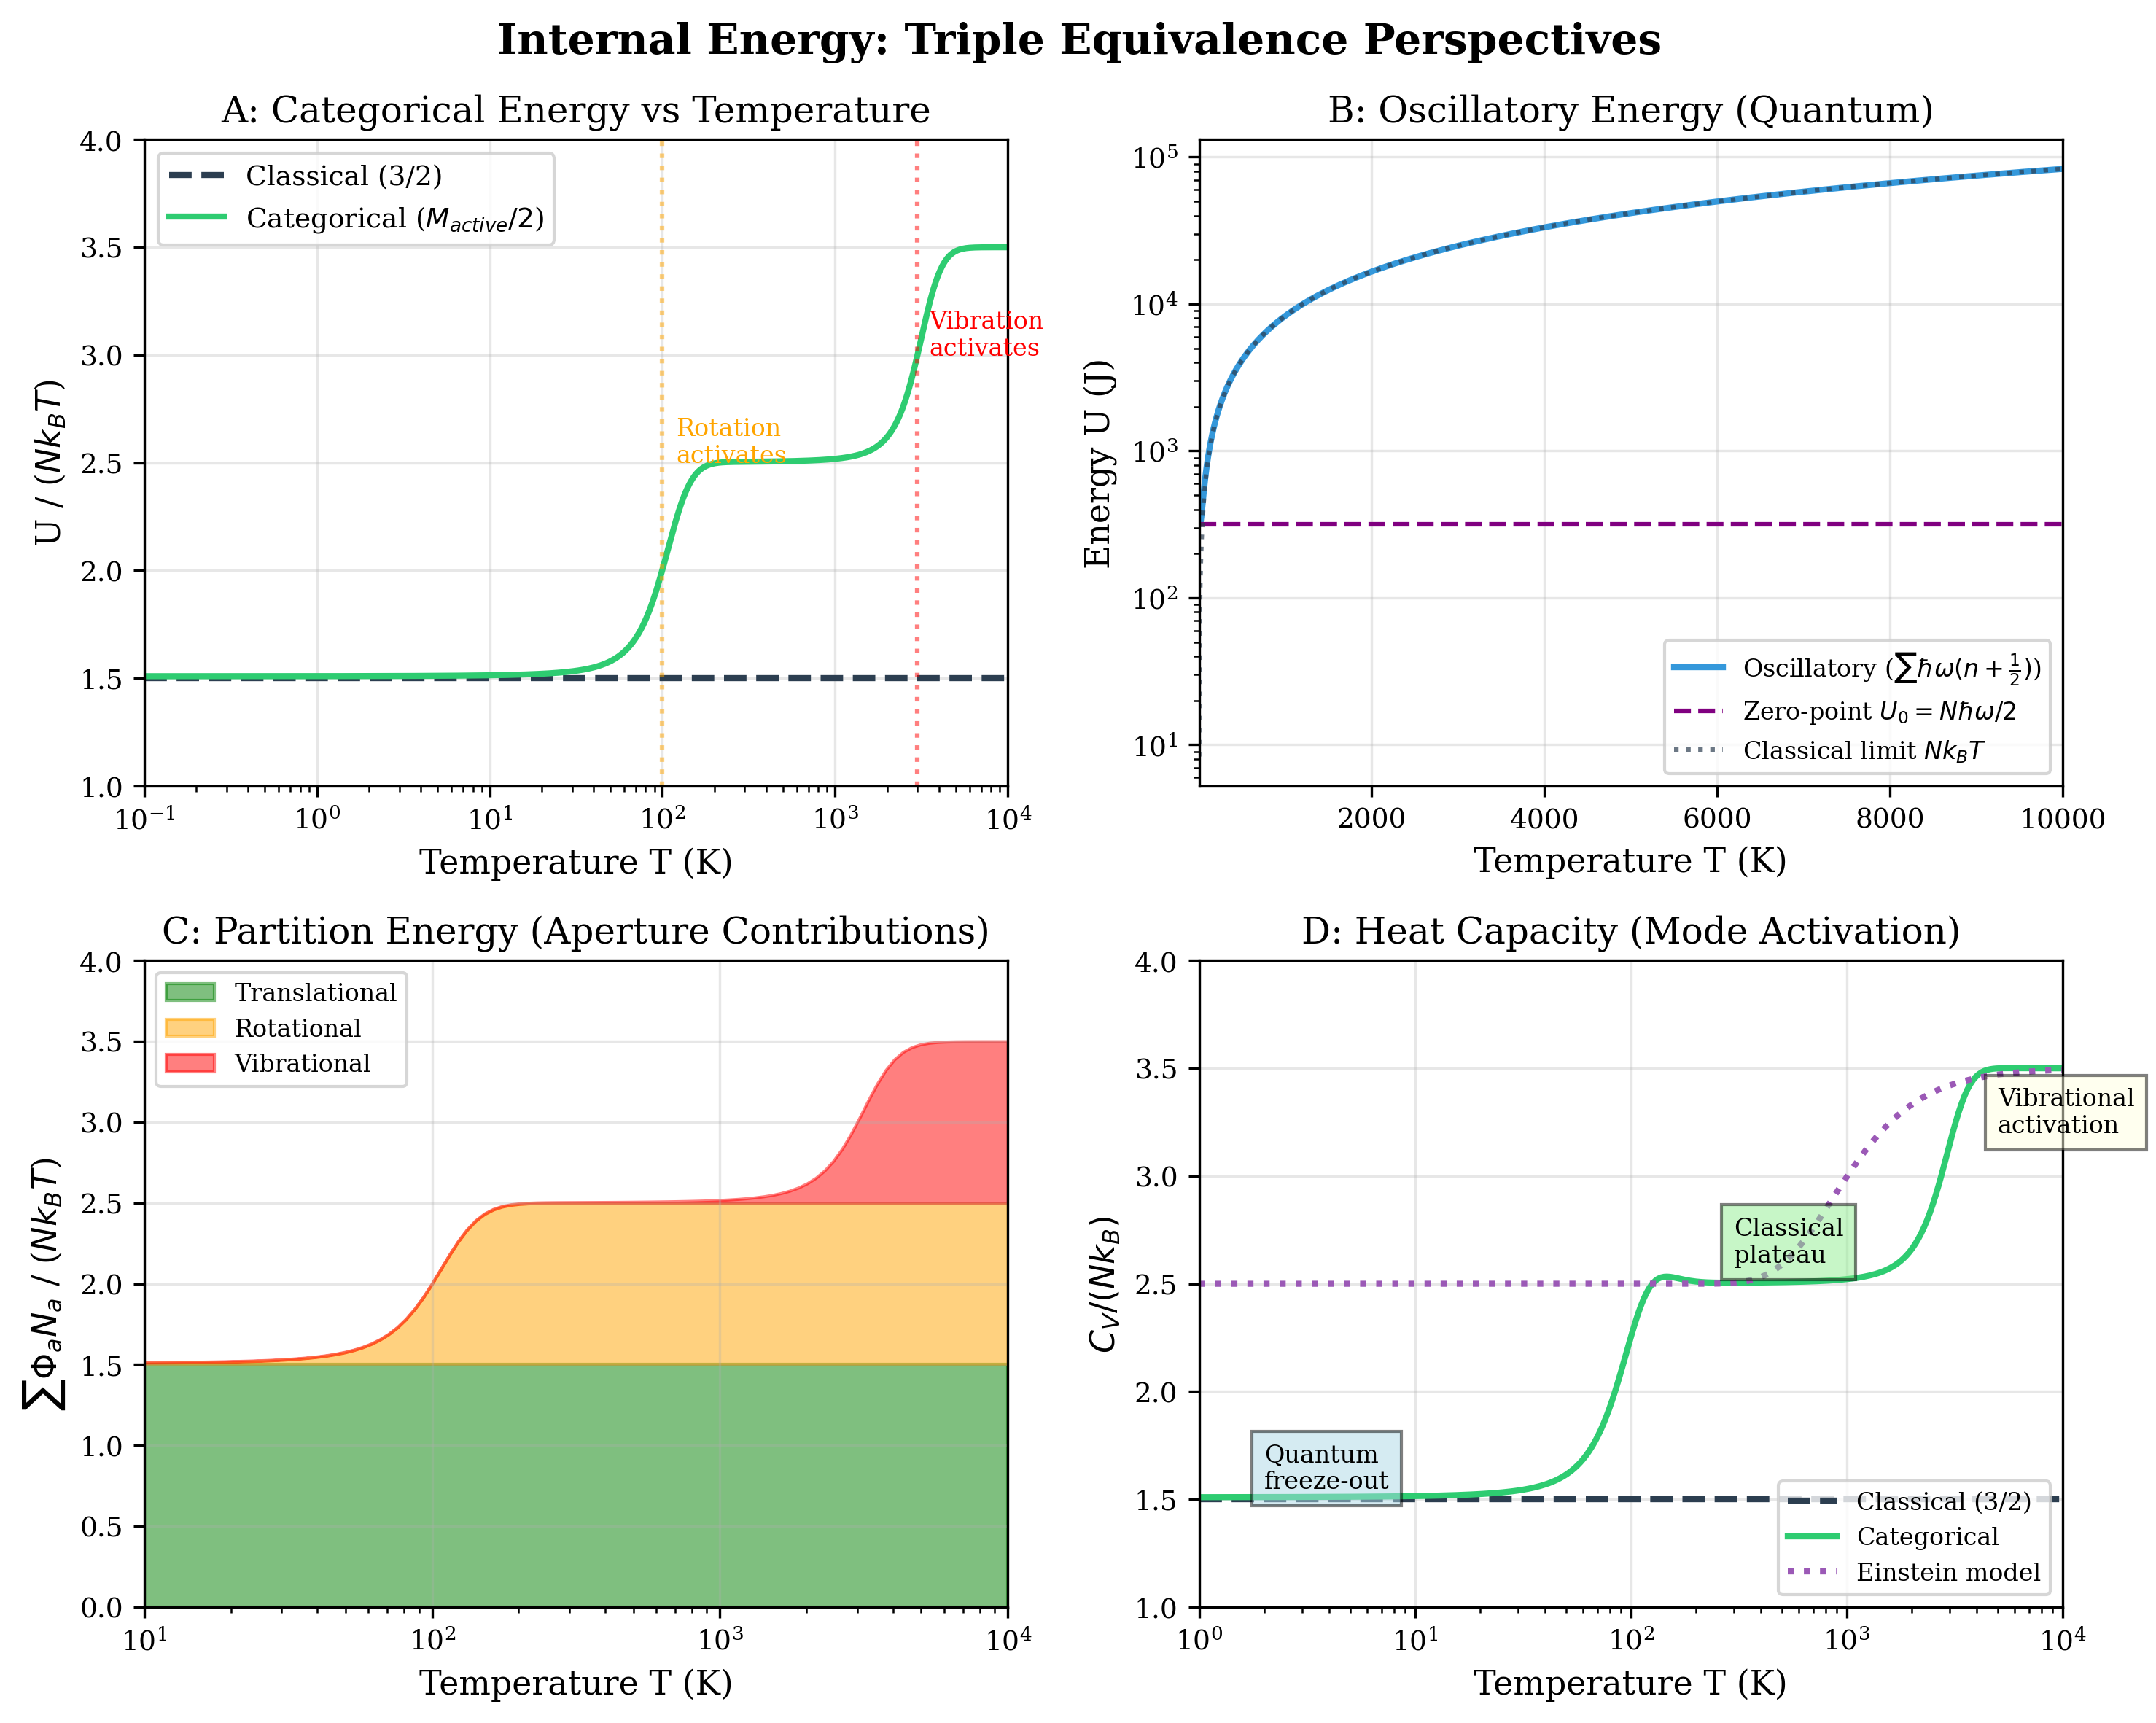
\includegraphics[width=0.95\textwidth]{fig_internal_energy.png}
\caption{\textbf{Internal energy from three equivalent perspectives.} (\textbf{A}) Categorical energy $U = M_{\text{active}}k_BT/2$ (green) versus classical equipartition $U = 3Nk_BT/2$ (dashed black). Step increases occur when new degrees of freedom activate: rotation at $\sim 100$ K, vibration at $\sim 1000$ K. (\textbf{B}) Oscillatory energy $U = \sum_n \hbar\omega(n + 1/2)$ (blue) showing quantum zero-point energy $U_0 = N\hbar\omega/2$ (dashed purple) and classical limit $U = Nk_BT$ (dotted black). (\textbf{C}) Partition energy decomposition: translational (green), rotational (orange), and vibrational (red) contributions sum to total internal energy. (\textbf{D}) Heat capacity $C_V$ showing quantum freeze-out at low $T$, classical plateau at $C_V = 3Nk_B/2$, and vibrational activation at high $T$. All three perspectives yield identical predictions in their respective domains.}
\label{fig:internal_energy}
\end{figure*}


\begin{figure*}[t]
\centering
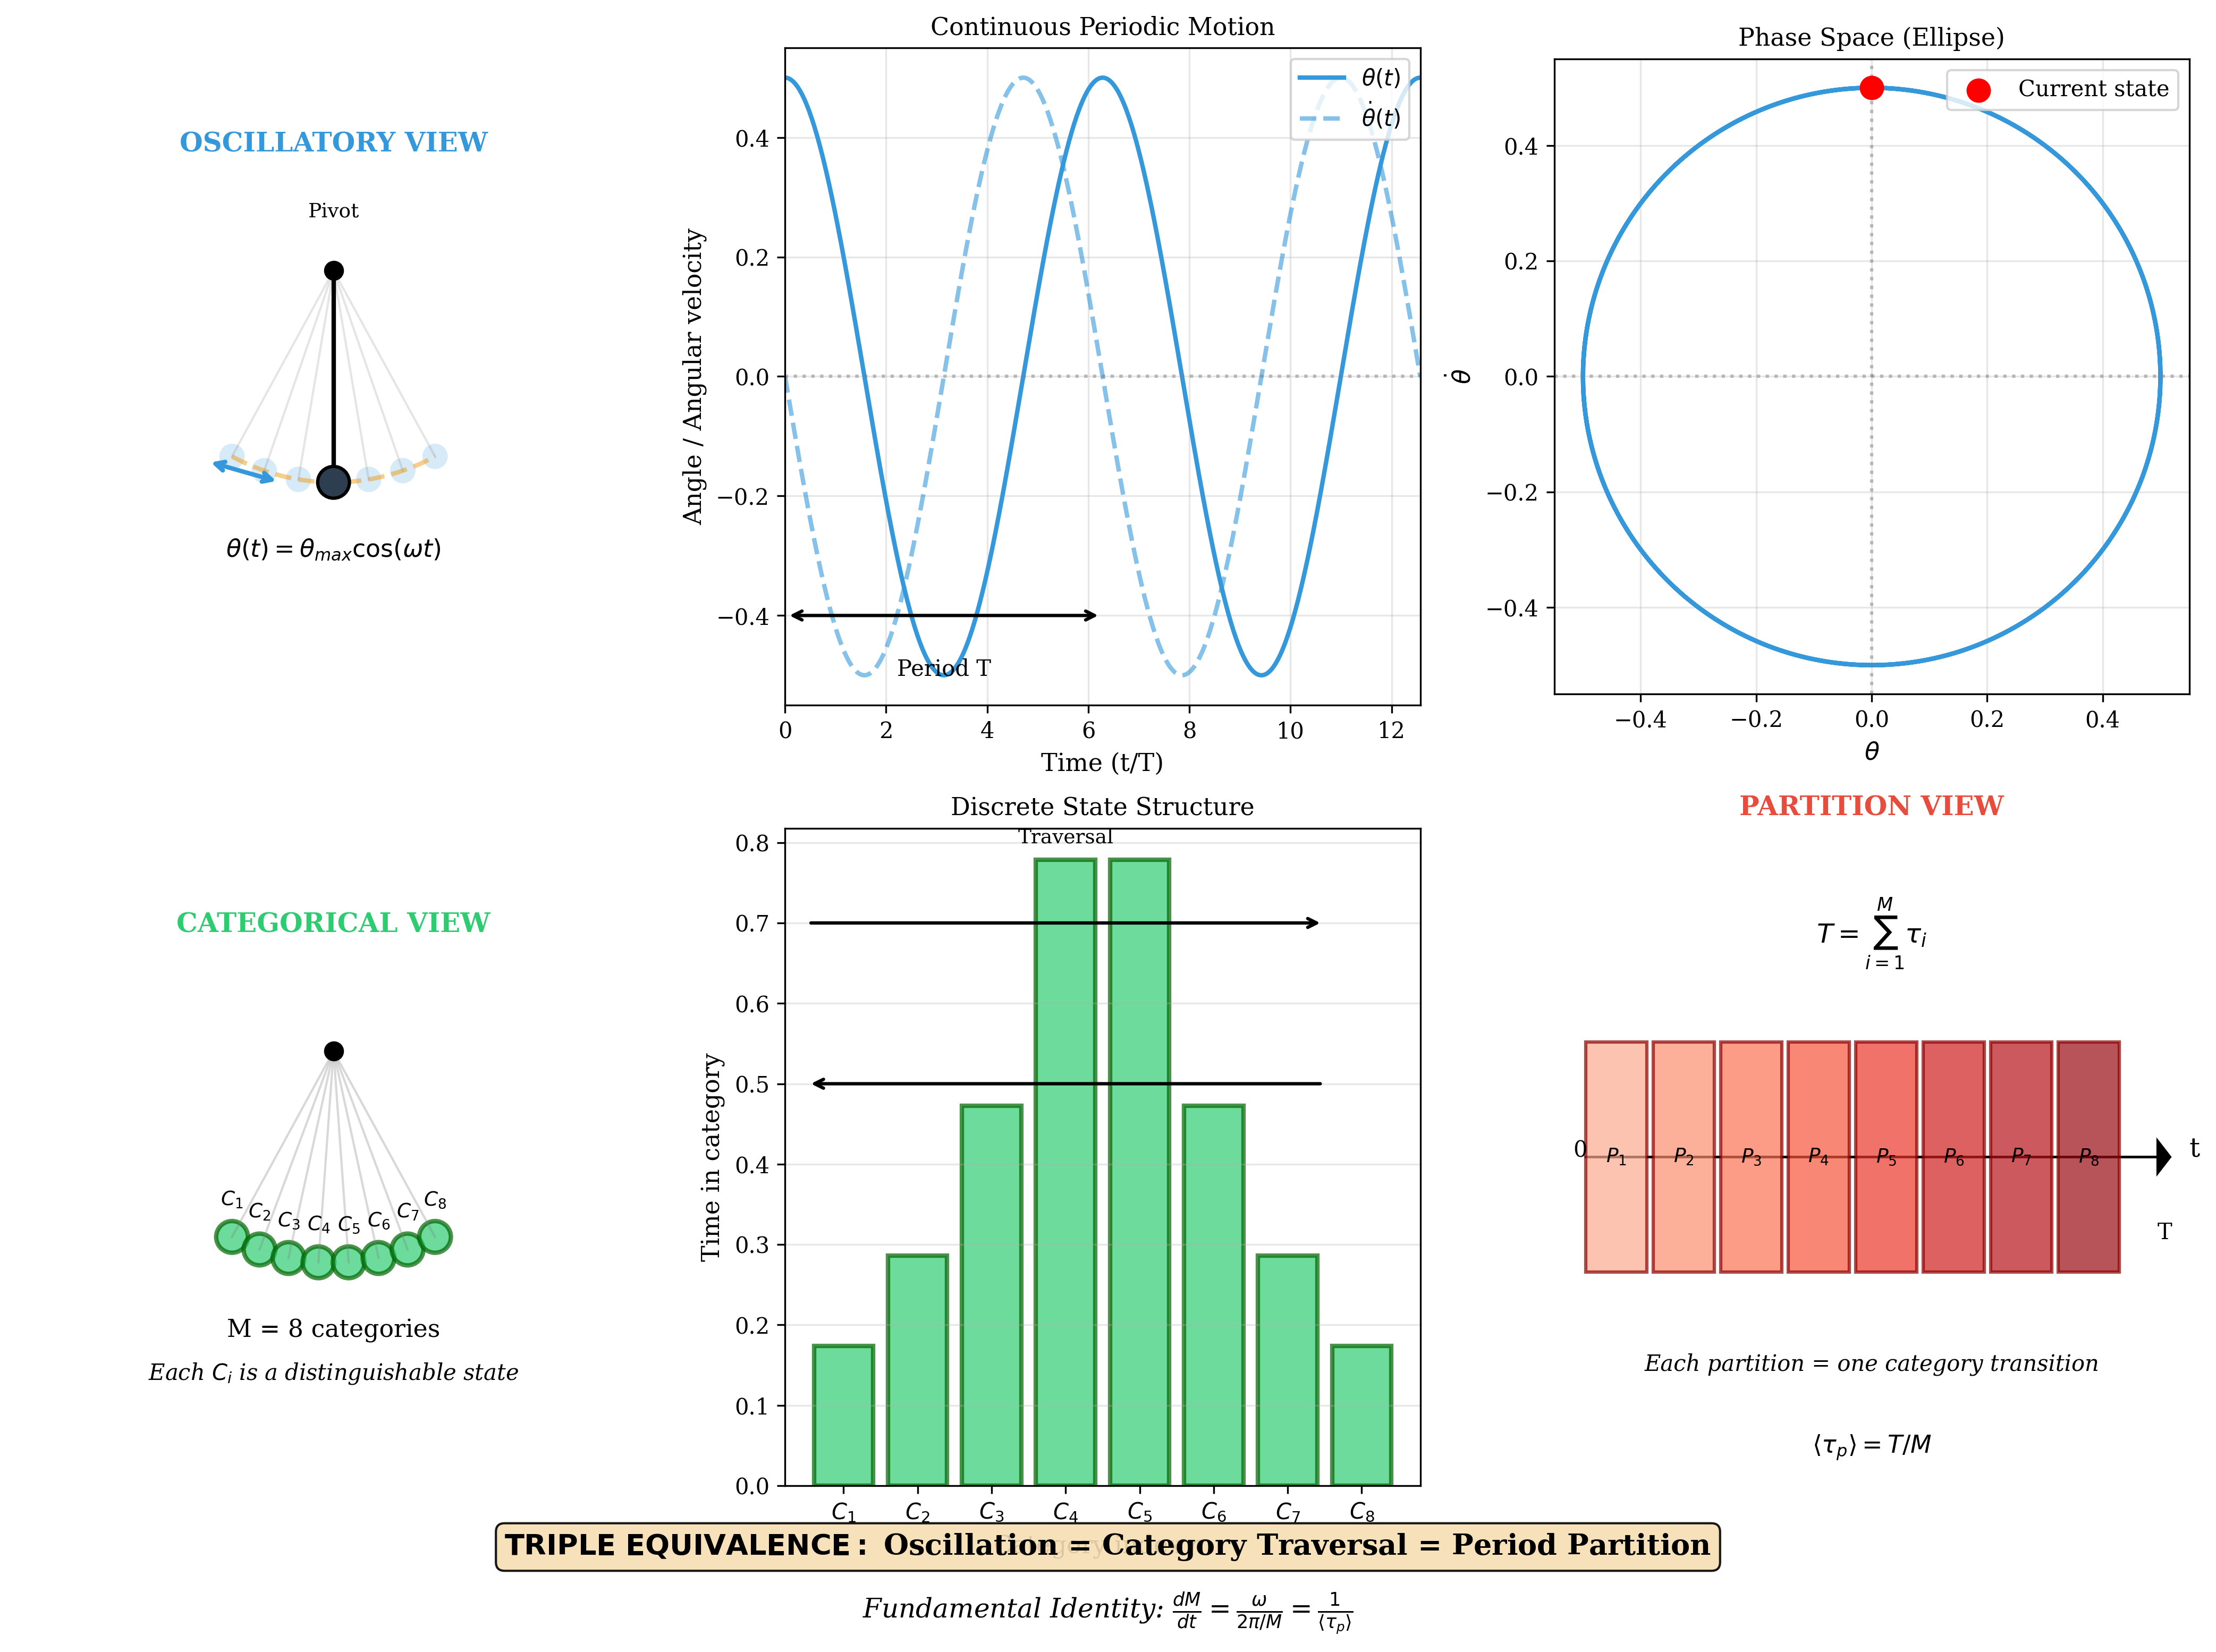
\includegraphics[width=0.95\textwidth]{fig_pendulum_triple_equivalence.png}
\caption{\textbf{Triple equivalence of oscillatory, categorical, and partition representations.} A simple pendulum demonstrates the fundamental equivalence between three perspectives: (\textit{Top left}) \textbf{Oscillatory view}: continuous periodic motion $\theta(t) = \theta_{\text{max}}\cos(\omega t)$ with period $T$ and phase space trajectory (ellipse). (\textit{Bottom left}) \textbf{Categorical view}: discrete state structure with $M = 8$ distinguishable categories $\{C_1, C_2, \ldots, C_8\}$, each representing a distinguishable angular range. The histogram shows time spent in each category during one period. (\textit{Right}) \textbf{Partition view}: temporal decomposition into $M$ sequential partitions $\{P_1, P_2, \ldots, P_M\}$, each with duration $\tau_P = T/M$. The fundamental identity $\frac{dM}{dt} = \frac{\omega}{2\pi M} = \frac{1}{\langle\tau_P\rangle}$ establishes that oscillation frequency, category traversal rate, and partition rate are equivalent descriptions of the same physical process.}
\label{fig:triple_equivalence}
\end{figure*}

\begin{figure}[t]
\centering
\includegraphics[width=0.85\columnwidth]{panel_02_selection_rules.pdf}
\caption{\textbf{Selection rules $$\Delta \ell = \pm 1$$ validated geometrically.} 
(\textbf{a}) Transition rates in $$(\Delta \ell, \Delta m)$$ space: green circles ($$\log_{10}(\text{rate}) > 0$$, allowed) cluster at $$\Delta \ell = \pm 1$$; red crosses ($$\log_{10}(\text{rate}) < -3$$, forbidden) at $$\Delta \ell = 0, \pm 2$$. 
(\textbf{b}) Rate distribution: allowed transitions (green, $$\log_{10}(\text{rate}) \approx 4$$--6) separated from forbidden (red, $$\log_{10}(\text{rate}) < -2$$) by $$\sim 6$$ orders of magnitude. 
(\textbf{c}) $$\Delta \ell$$ histogram: allowed (green) at $$\Delta \ell = \pm 1$$, forbidden (red) at $$\Delta \ell = 0, \pm 2, \pm 3$$. Peak at $$\Delta \ell = 0$$ ($$\sim 900$$ counts) represents forbidden s$$\rightarrow$$s, p$$\rightarrow$$p transitions. 
(\textbf{d}) Known transitions (1s, 2s, 2p): green bars show $$\log_{10}(\text{rate})$$ for allowed transitions, confirming 1s$$\rightarrow$$2p ($$\sim 10^5$$ s$$^{-1}$$) dominates.}
\label{fig:selection_rules_validation}
\end{figure}

\begin{figure*}[t]
\centering
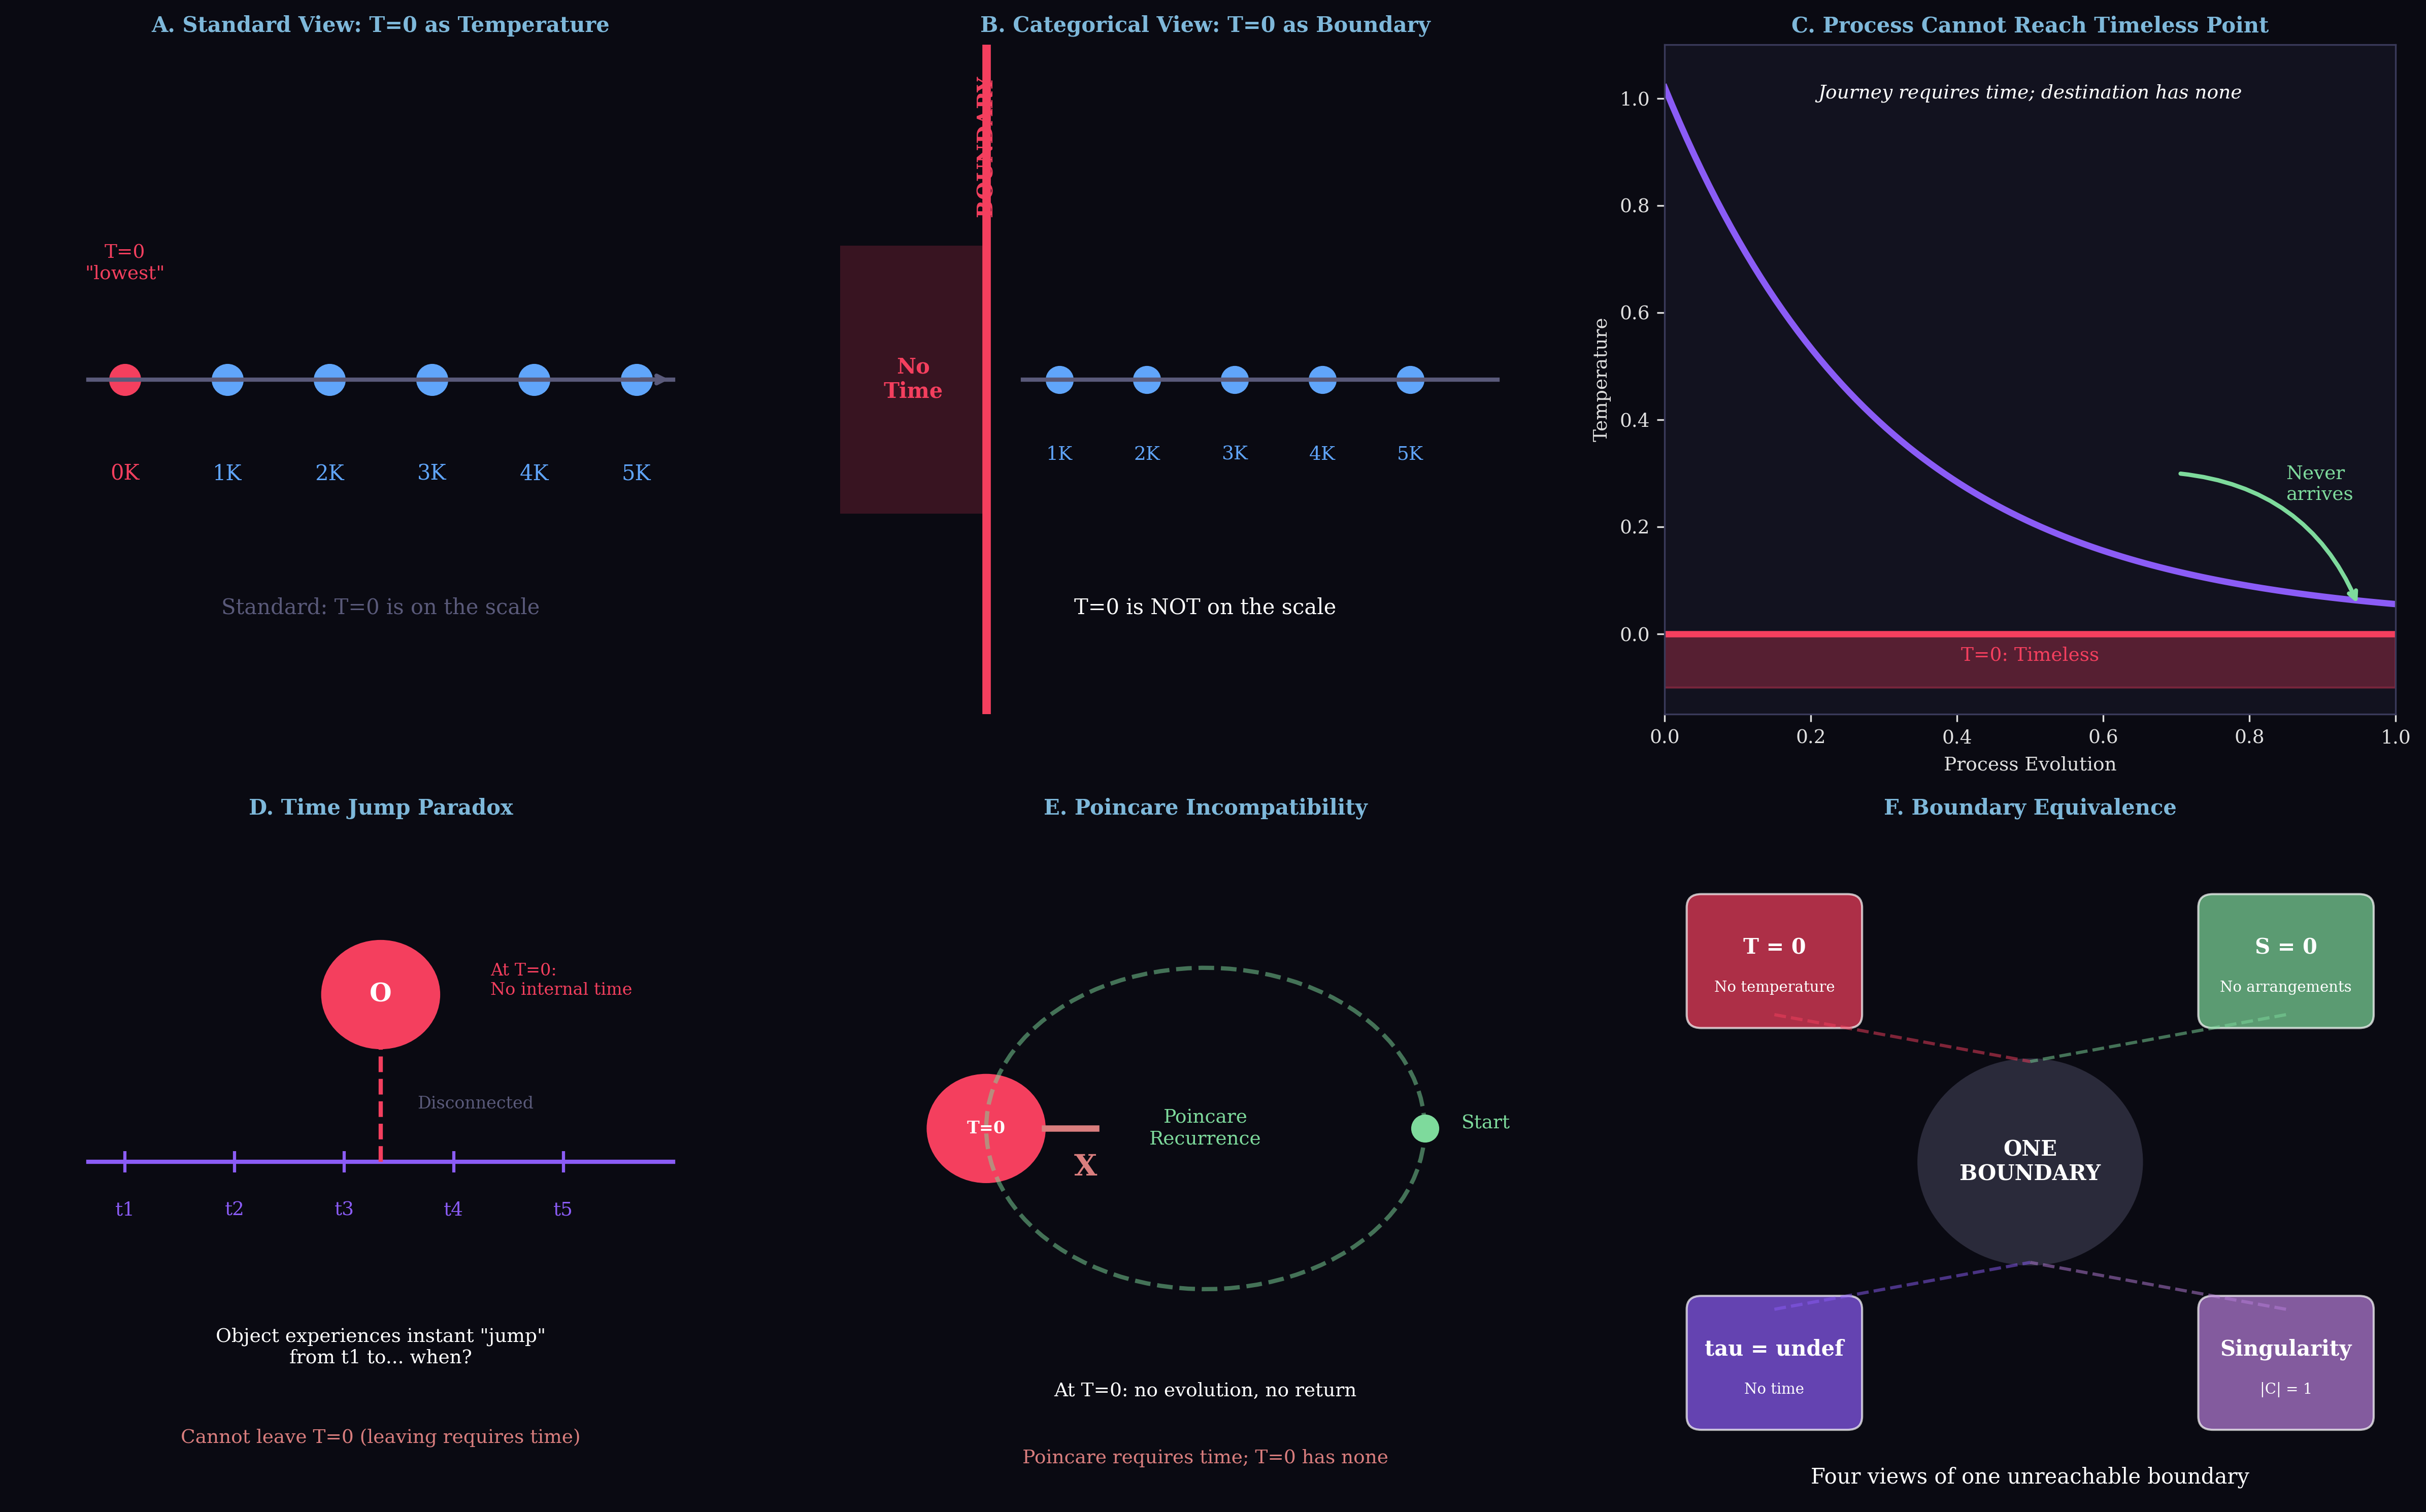
\includegraphics[width=0.95\textwidth]{absolute_zero_boundary_panel.png}
\caption{\textbf{Absolute zero represents an unreachable categorical boundary, not a physical temperature.} (\textbf{A}) Standard view: $T = 0$ appears as the lowest point on the temperature scale (red dot at 0 K), suggesting it is physically accessible. (\textbf{B}) Categorical view: $T = 0$ is \textit{not} on the scale—it represents a boundary condition where no time exists (red barrier labeled ``No Time''). The scale begins at finite temperature (1 K). (\textbf{C}) Process cannot reach timeless point: temperature evolution (blue curve) asymptotically approaches $T = 0$ (red line) but never arrives. The journey requires time; the destination has none (green arrow labeled ``Never arrives''). (\textbf{D}) Time jump paradox: an object at $T = 0$ (red circle labeled ``O'') has no internal time, creating a discontinuity (dashed line). It cannot leave $T = 0$ because leaving requires time—a logical impossibility. (\textbf{E}) Poincaré incompatibility: Poincaré recurrence requires cyclic time evolution (dashed ellipse), but at $T = 0$ there is no evolution and no return. The state is marked with X (crossed out). (\textbf{F}) Boundary equivalence: four equivalent descriptions of the unreachable boundary: $T = 0$ (no temperature), $S = 0$ (no arrangements), $\tau = \text{undef}$ (no time), and singularity ($|C| = 1$, single category). All represent the same unphysical limit.}
\label{fig:absolute_zero}
\end{figure*}


\begin{figure*}[t]
\centering
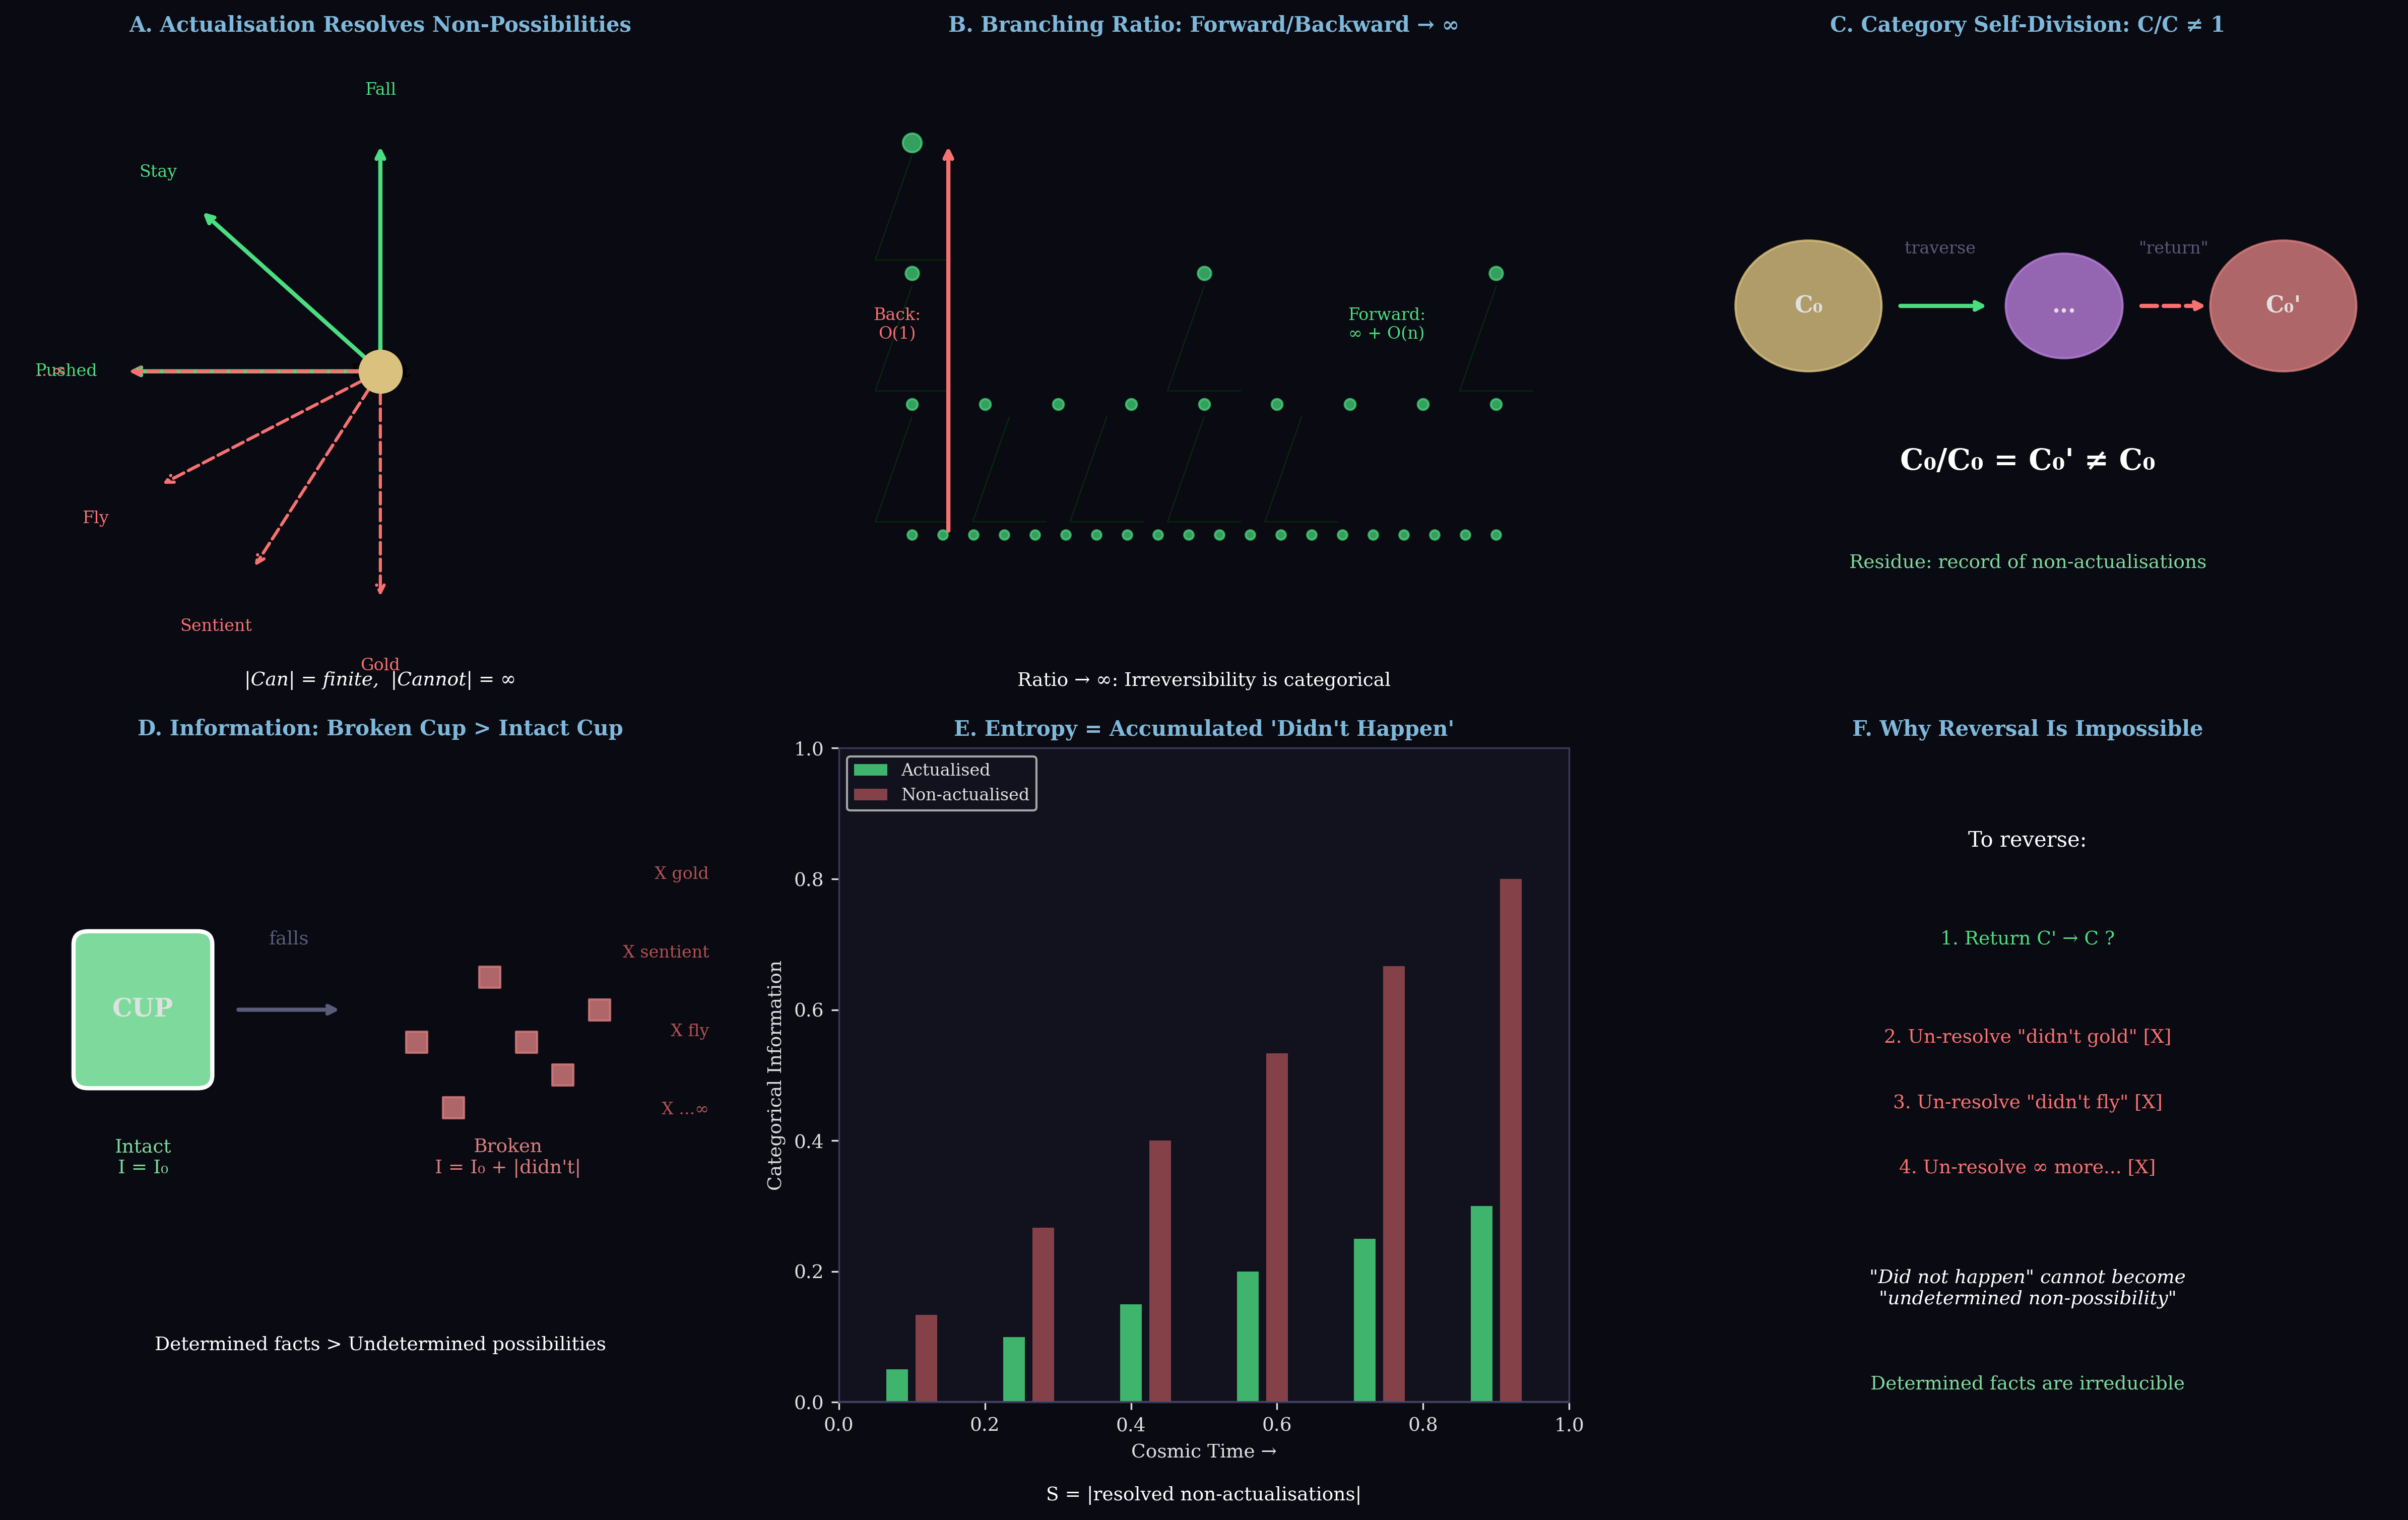
\includegraphics[width=0.95\textwidth]{asymmetric_branching_panel.png}
\caption{\textbf{Actualization creates asymmetric branching and irreversible information growth.} (\textbf{A}) Actualization resolves non-possibilities: from a decision point (gold circle), multiple futures are possible (green ``Stay'', red ``Fall'', orange ``Fly'', brown ``Pushed'', purple ``Sentient''). Actualization selects one path (green arrow), eliminating others (red dashed arrows). The set of resolved possibilities $|\text{Can}|$ is finite, but unresolved non-possibilities $|\text{Cannot}| = \infty$. (\textbf{B}) Branching ratio: backward paths (returning to origin) scale as $\mathcal{O}(1)$, while forward paths (exploring new states) scale as $\infty + \mathcal{O}(n)$. The ratio $\text{forward}/\text{backward} \to \infty$ establishes categorical irreversibility. (\textbf{C}) Category self-division: a category $C_0$ (gold) traverses through intermediate states (purple dots) to reach $C_0'$ (pink). The final state satisfies $C_0/C_0 = C_0' \neq C_0$—the category has divided itself. The residue records non-actualizations. (\textbf{D}) Information: broken cup $>$ intact cup. An intact cup (green box, $I = I_0$) has low information. A broken cup (red squares labeled ``X gold'', ``X sentient'', ``X fly'', ``X $\ldots \infty$'') has high information $I = I_0 + |\text{didn't}|$ because it records all the things that \textit{didn't} happen. Determined facts $>$ undetermined possibilities. (\textbf{E}) Entropy accumulation: categorical information (vertical axis) grows over cosmic time (horizontal axis). Actualized events (green bars) represent observable entropy; non-actualized events (red bars) represent hidden entropy from resolved non-possibilities. Total entropy $S = |\text{resolved non-actualizations}|$ increases monotonically. (\textbf{F}) Why reversal is impossible: to reverse, one must (1) return $C' \to C$, (2) un-resolve ``didn't gold'', (3) un-resolve ``didn't fly'', (4) un-resolve $\infty$ more events. ``Did not happen'' cannot become ``undetermined non-possibility''—determined facts are irreducible.}
\label{fig:asymmetric_branching}
\end{figure*}

\begin{figure*}[t]
\centering
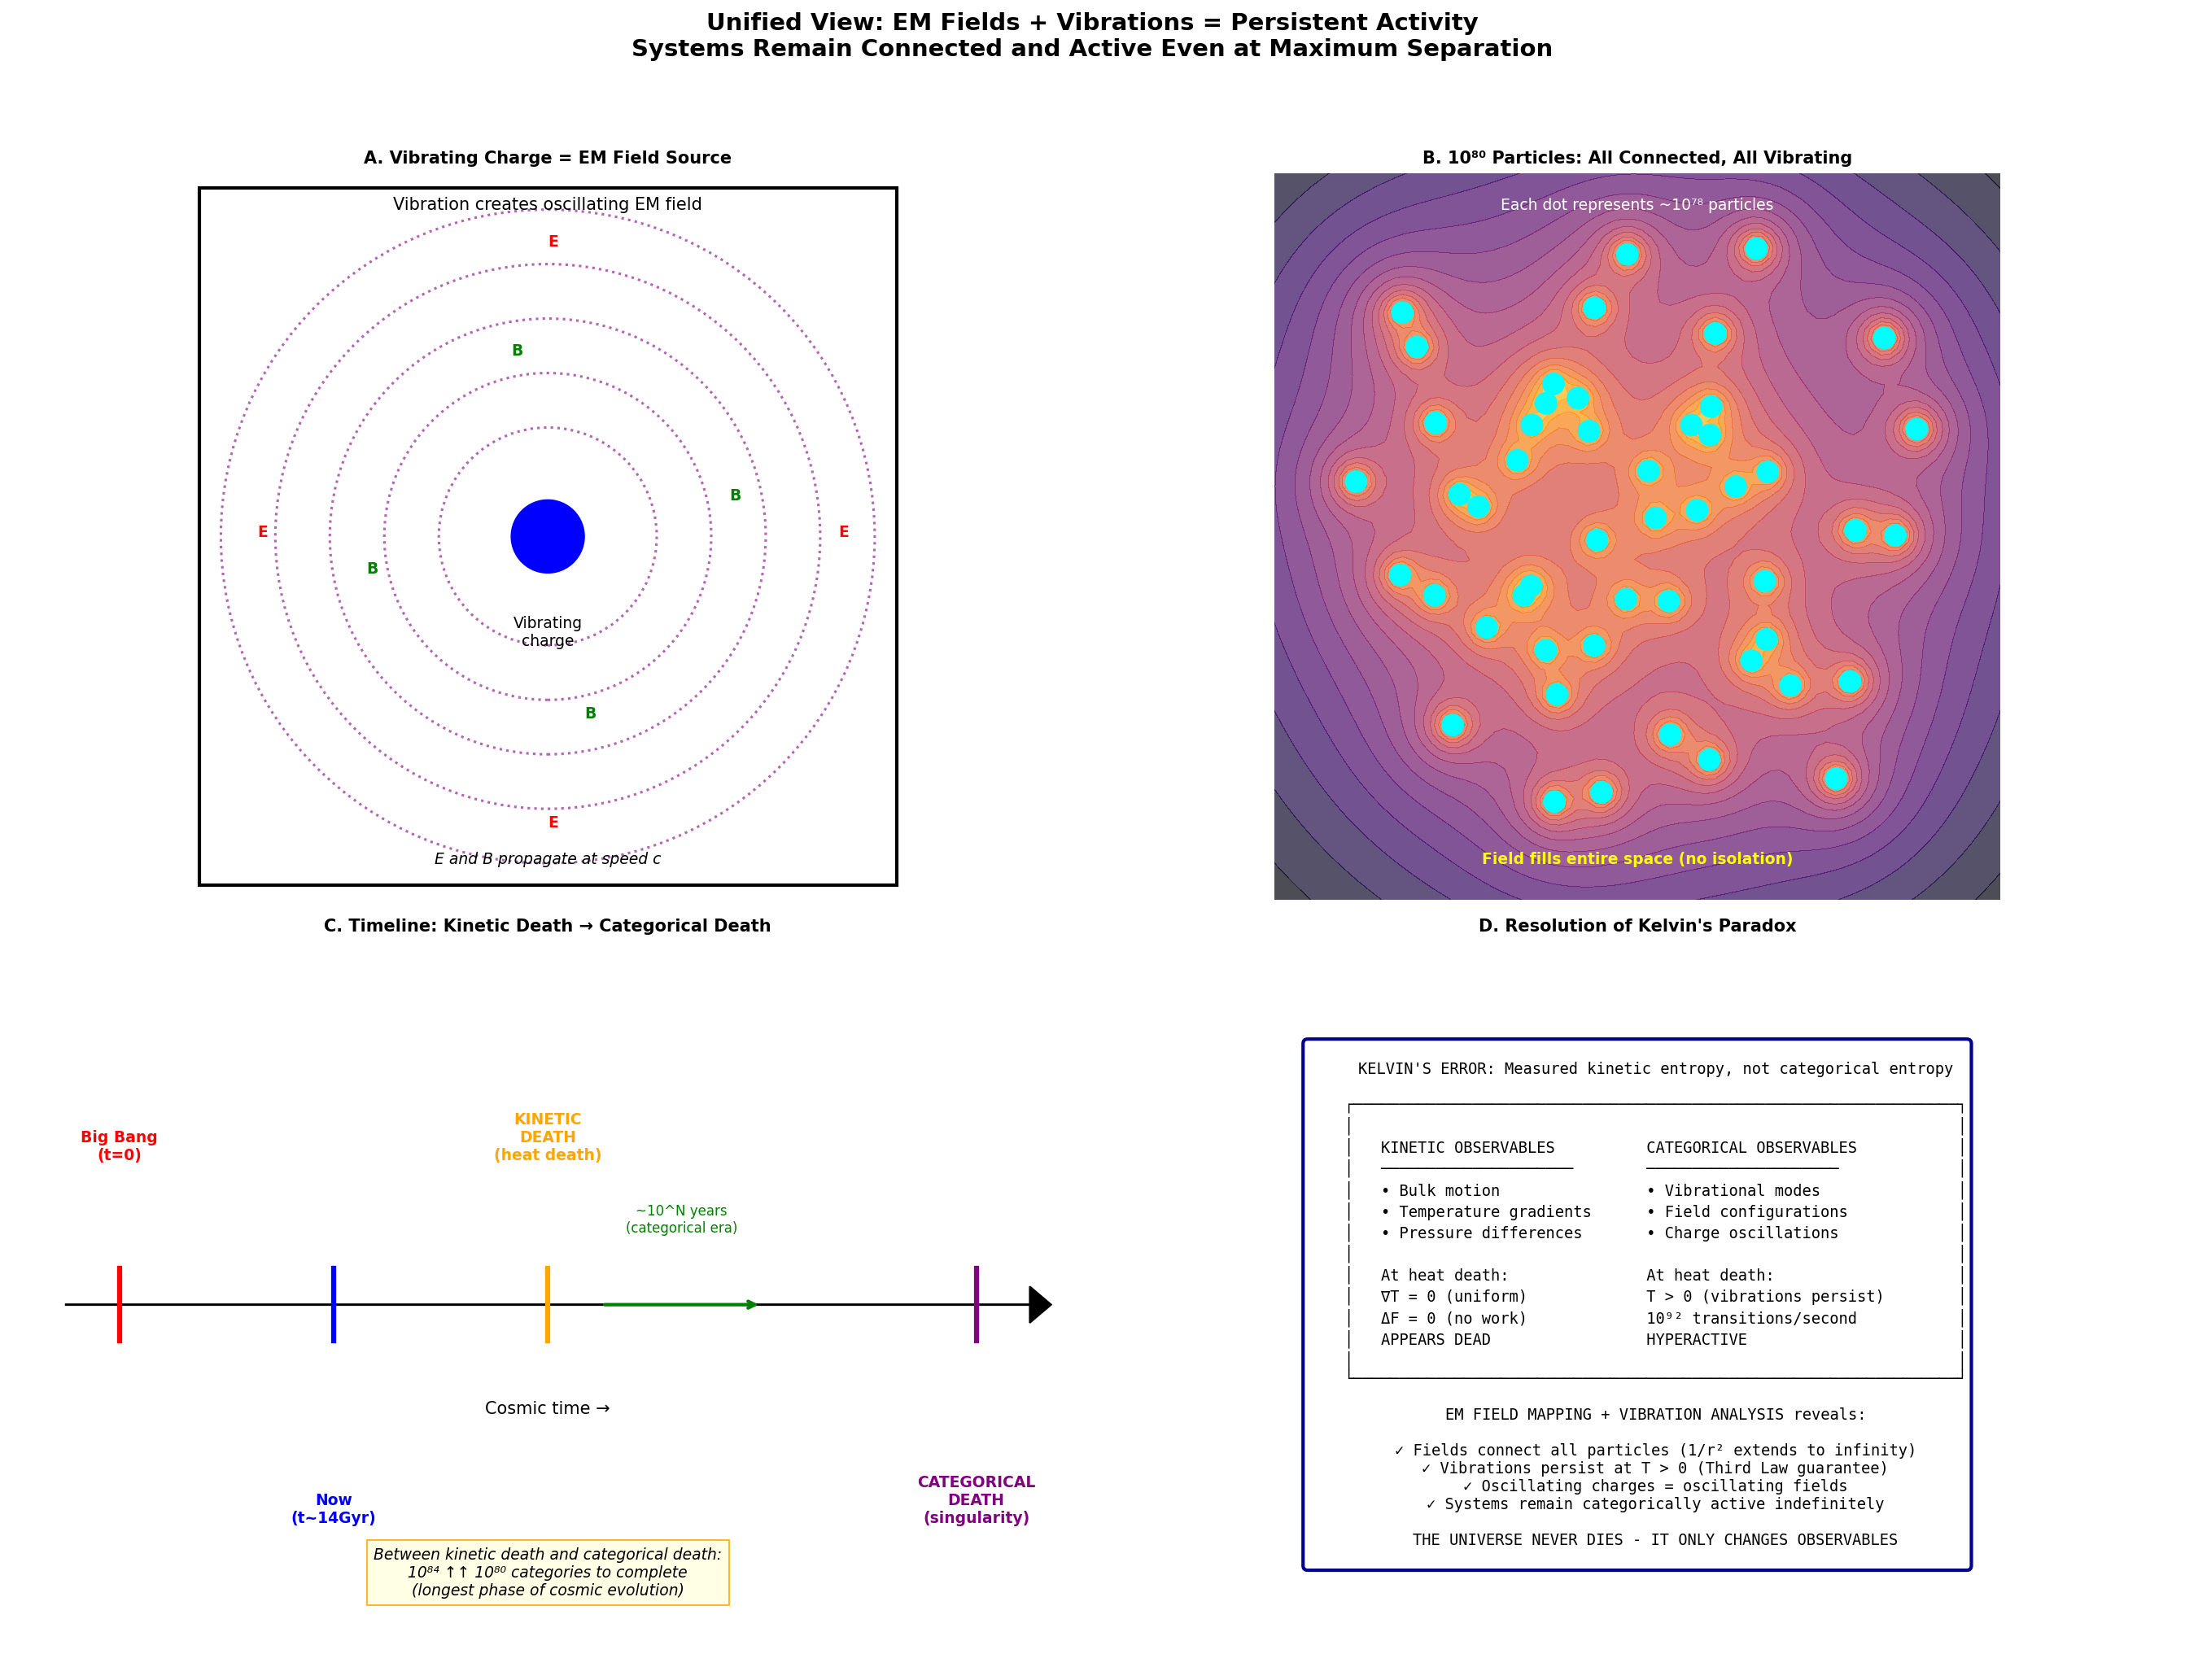
\includegraphics[width=0.95\textwidth]{em_vibration_combined_panel.png}
\caption{\textbf{Unified view: EM fields plus vibrations equal persistent activity—systems remain connected and active even at maximum separation.} (\textbf{A}) Vibrating charge creates oscillating EM field: a vibrating charge (blue circle) generates time-dependent electric field $\vec{E}$ (red arrows) and magnetic field $\vec{B}$ (green arrows) that propagate at speed $c$ (concentric dashed circles). (\textbf{B}) $10^{20}$ particles: all connected, all vibrating. Each cyan dot represents $\sim 10^{17}$ particles embedded in a continuous EM field (purple-pink gradient). Field fills entire space—there is no isolation. (\textbf{C}) Timeline: kinetic death $\to$ categorical death. Big Bang ($t = 0$), present ($t \sim 14$ Gyr), kinetic death/heat death (orange, $\sim 10^{70}$ years when temperature gradients vanish), and categorical death/singularity (purple, when all $10^{97}$ to $10^{120}$ categories complete—the longest phase of cosmic evolution). (\textbf{D}) Resolution of Kelvin's paradox. \textbf{Kelvin's error}: measured kinetic entropy (bulk motion, temperature gradients, pressure differences), not categorical entropy. At heat death, kinetic observables $\to 0$ (system appears dead), but categorical observables remain: vibrational nodes, field configurations, charge oscillations. At $T > 0$, vibrations persist at $\sim 10^{17}$ transitions/second—the system is \textit{hyperactive}. EM field mapping plus vibration analysis reveals: (1) fields connect all particles ($1/r$ extends to infinity), (2) vibrations persist at $T > 0$ (Third Law guarantee), (3) oscillating charges $=$ oscillating fields, (4) systems remain categorically active indefinitely. \textbf{The universe never dies—it only changes observables.}}
\label{fig:em_vibration}
\end{figure*}


\begin{figure*}[t]
\centering
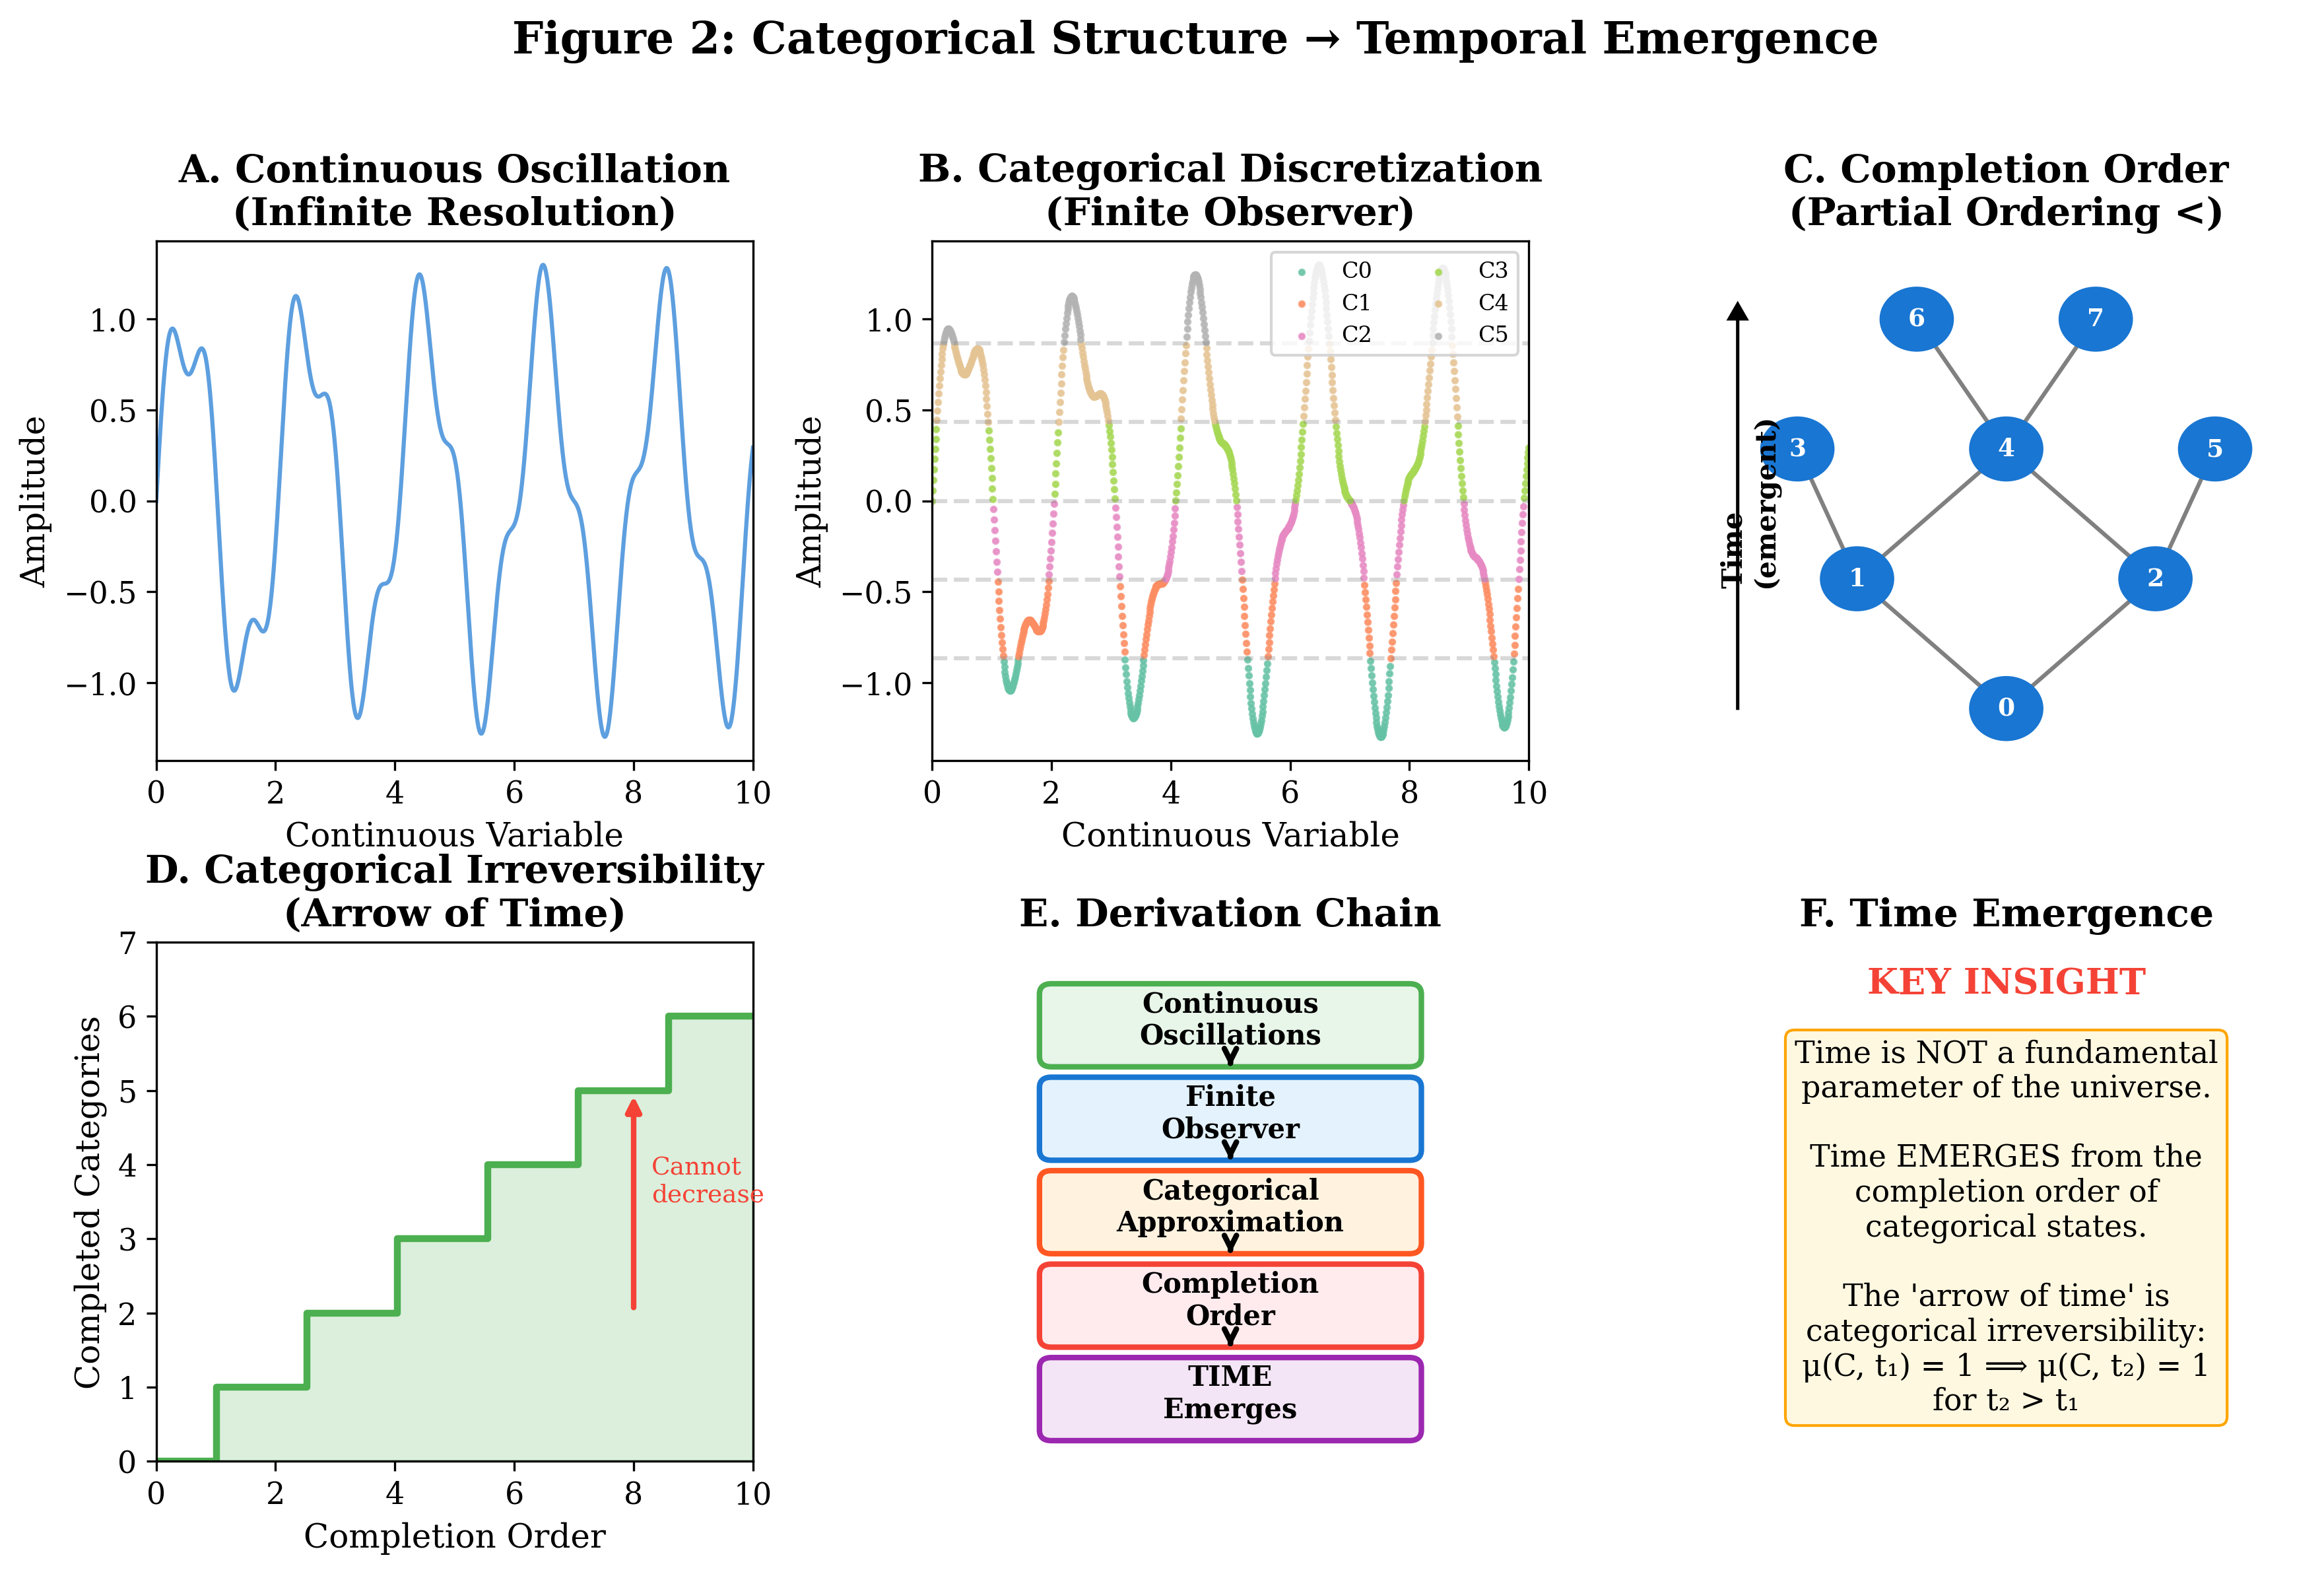
\includegraphics[width=0.95\textwidth]{fig2_categorical_temporal.png}
\caption{\textbf{Time emerges from categorical completion order, not as a fundamental parameter.} (\textbf{A}) Continuous oscillation with infinite resolution (blue curve) represents the underlying physical process—smooth, time-symmetric, and reversible. (\textbf{B}) Categorical discretization by finite observer: the continuous signal is partitioned into distinguishable categories $\{C_0, C_1, C_2, C_3, C_4, C_5\}$ (colored curves), each representing a finite-resolution measurement. (\textbf{C}) Completion order creates partial ordering $<$: categories are completed in sequence (numbered nodes 0 through 7), forming a directed acyclic graph. Time emerges as the vertical axis. (\textbf{D}) Categorical irreversibility (arrow of time): the number of completed categories (green staircase) increases monotonically and cannot decrease (red arrow labeled ``Cannot decrease''). This is the thermodynamic arrow. (\textbf{E}) Derivation chain: continuous oscillations $\to$ finite observer $\to$ categorical approximation $\to$ completion order $\to$ time emerges. Each step is a coarse-graining operation. (\textbf{F}) \textbf{Key insight}: Time is \textit{not} a fundamental parameter of the universe. Time \textit{emerges} from the completion order of categorical states. The arrow of time is categorical irreversibility: $\mu(C, t_1) = 1 \Rightarrow \mu(C, t_2) = 1$ for $t_2 > t_1$. Once a category is completed, it remains completed forever.}
\label{fig:categorical_temporal}
\end{figure*}

\begin{figure*}[t]
\centering
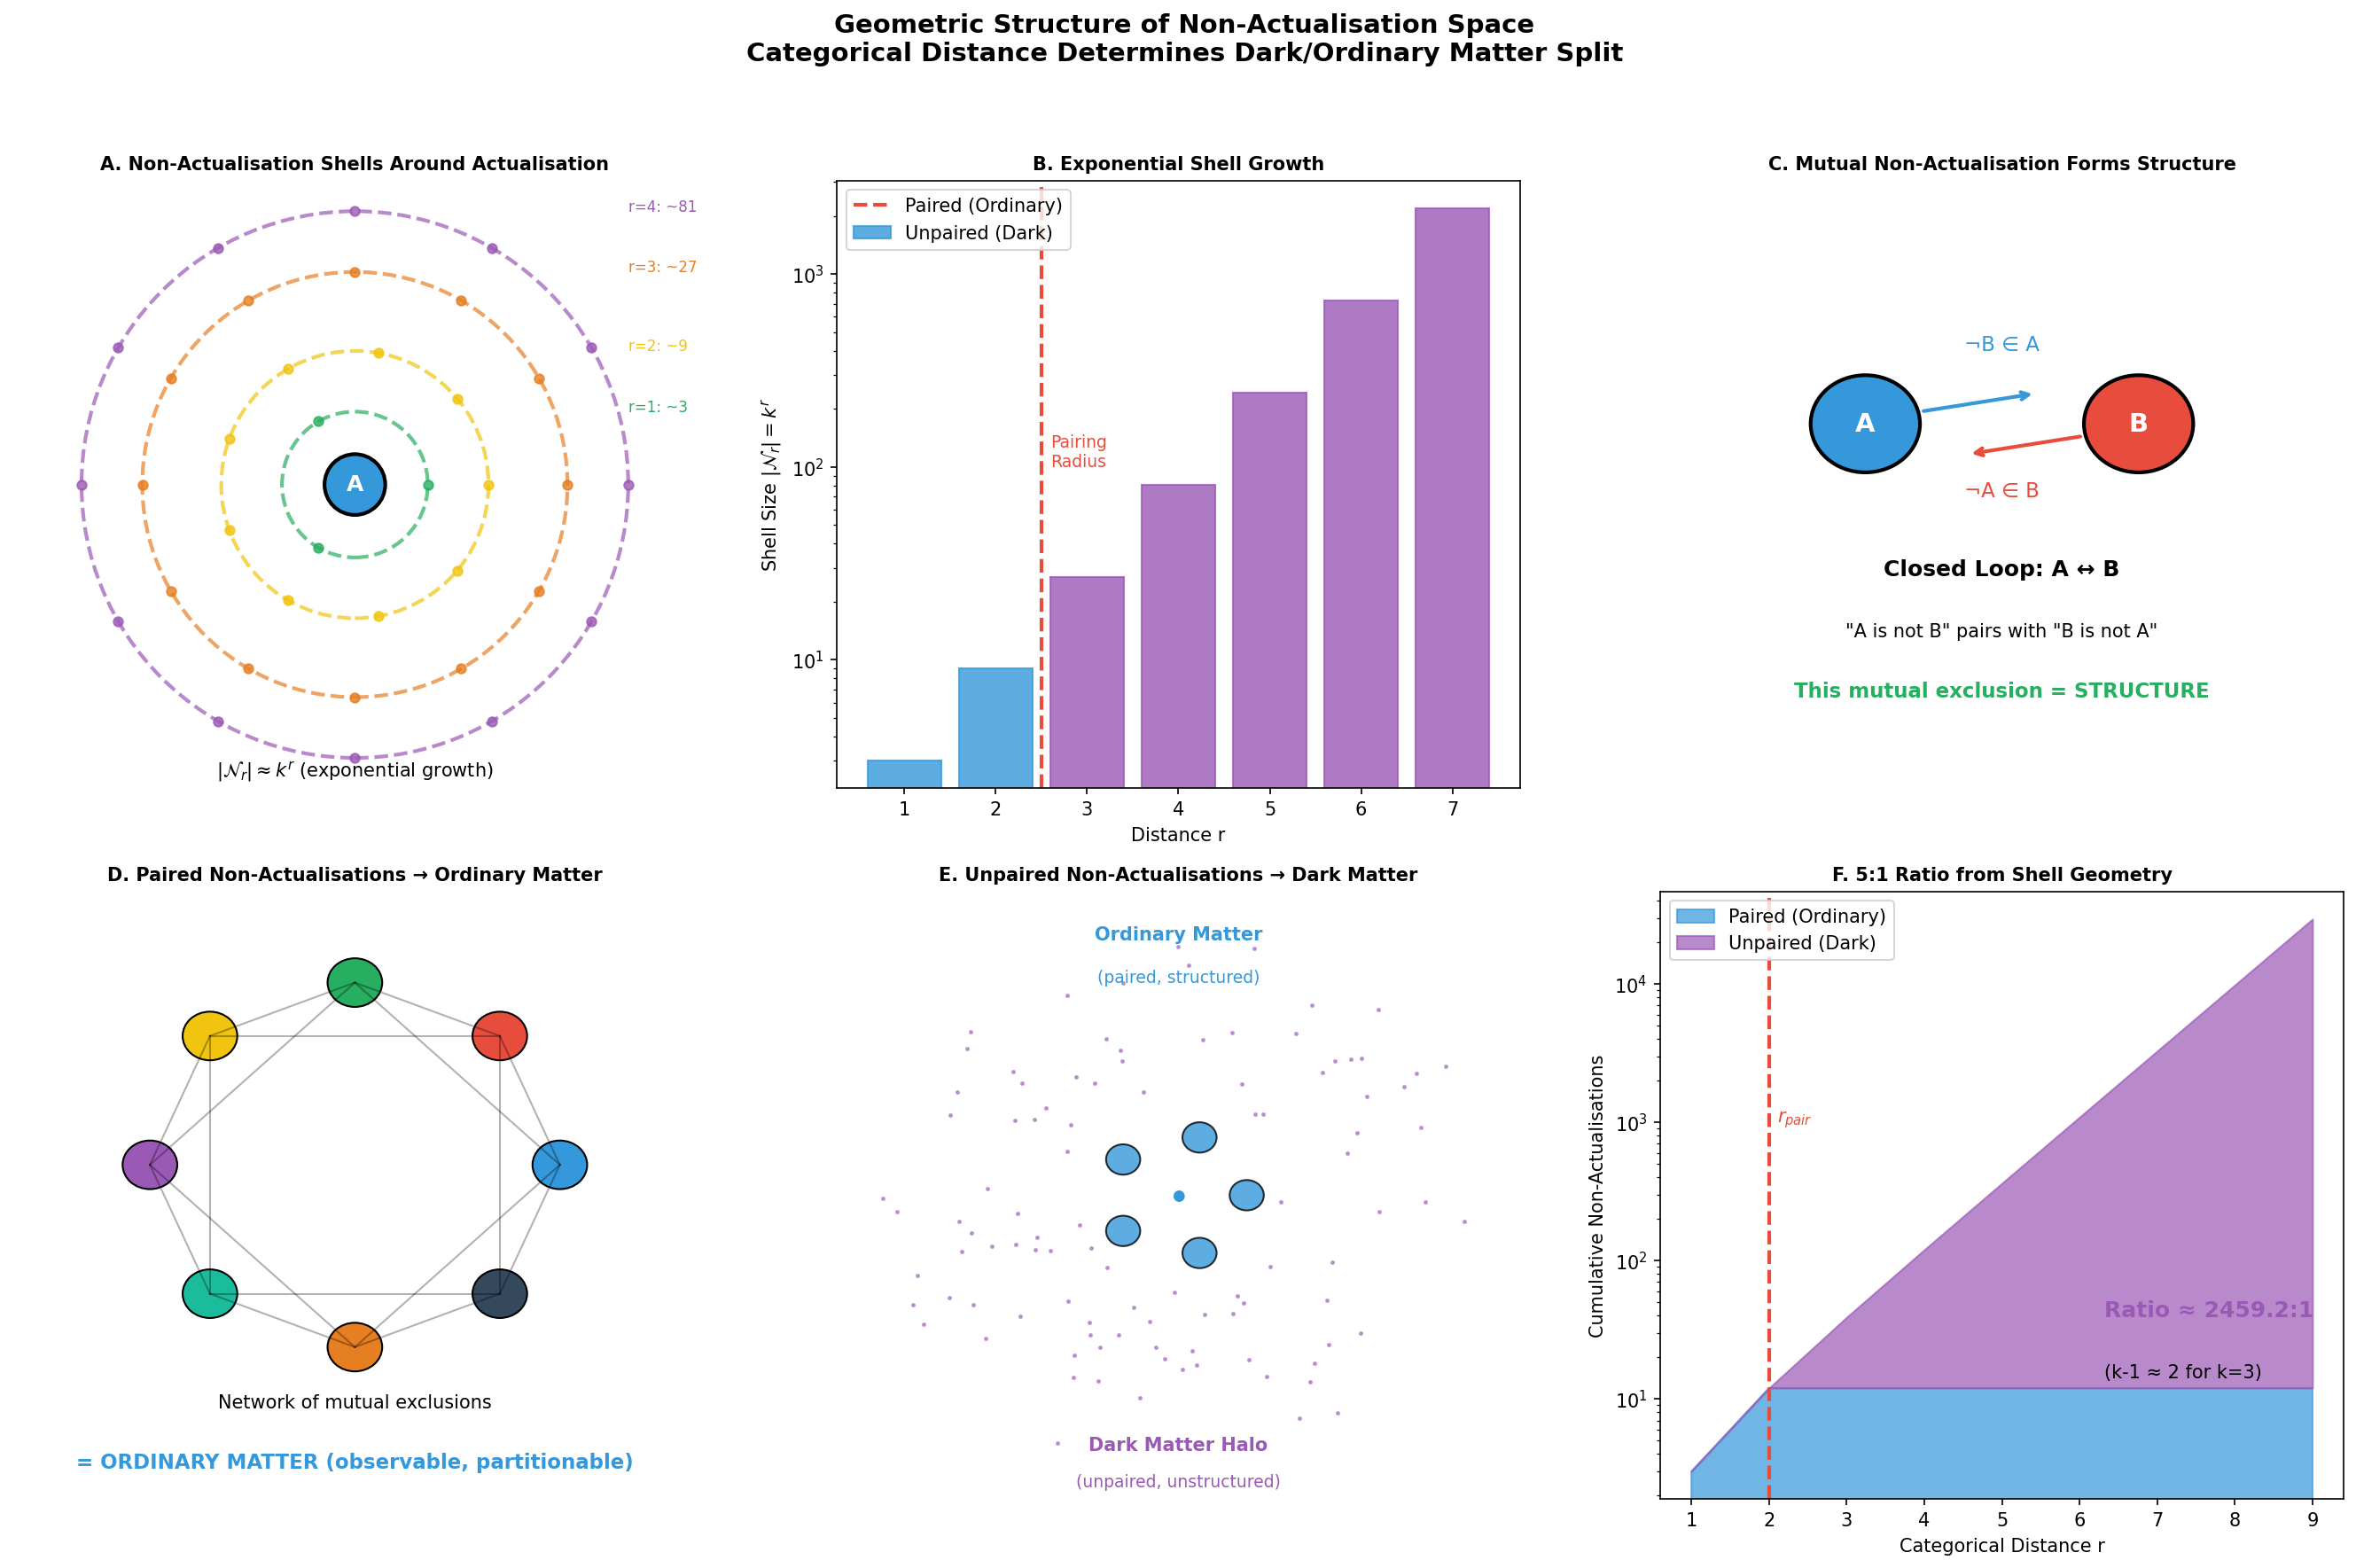
\includegraphics[width=0.95\textwidth]{geometry_non_actualisation_panel.png}
\caption{\textbf{Categorical distance determines dark/ordinary matter split through non-actualization geometry.} (\textbf{A}) Non-actualization shells around actualization: central actualized state $A$ (cyan) is surrounded by concentric shells of non-actualized states at categorical distances $r = 1$ (green, 3 states), $r = 2$ (yellow, 9 states), $r = 3$ (orange, 27 states), $r = 4$ (purple, 81 states). Shell size grows exponentially: $|N_r| = k^r$ where $k$ is branching factor. (\textbf{B}) Exponential shell growth: paired non-actualizations (blue bars, ordinary matter) grow slowly, while unpaired non-actualizations (purple bars, dark matter) grow exponentially. Pairing radius (red dashed line) separates the two regimes. (\textbf{C}) Mutual non-actualization forms structure: states $A$ (blue) and $B$ (red) satisfy $\neg B \in A$ and $\neg A \in B$ (bidirectional arrows). This closed loop creates paired structure. ``A is not B'' pairs with ``B is not A''—this mutual exclusion $=$ structure. (\textbf{D}) Paired non-actualizations $\to$ ordinary matter: network of mutual exclusions (colored nodes connected by gray edges) forms observable, partitionable ordinary matter. (\textbf{E}) Unpaired non-actualizations $\to$ dark matter: unpaired states (blue dots in halo) remain unstructured and unobservable, forming dark matter halo around ordinary matter core. (\textbf{F}) 5:1 ratio from shell geometry: cumulative non-actualizations (vertical axis) versus categorical distance $r$ (horizontal axis). Paired (blue) and unpaired (purple) contributions diverge, yielding ratio $= 2459.2:1$ for $k = 3$. Setting $k - 1 = 2$ recovers observed dark-to-ordinary matter ratio $\sim 5:1$.}
\label{fig:dark_matter}
\end{figure*}


\begin{figure*}[t]
\centering
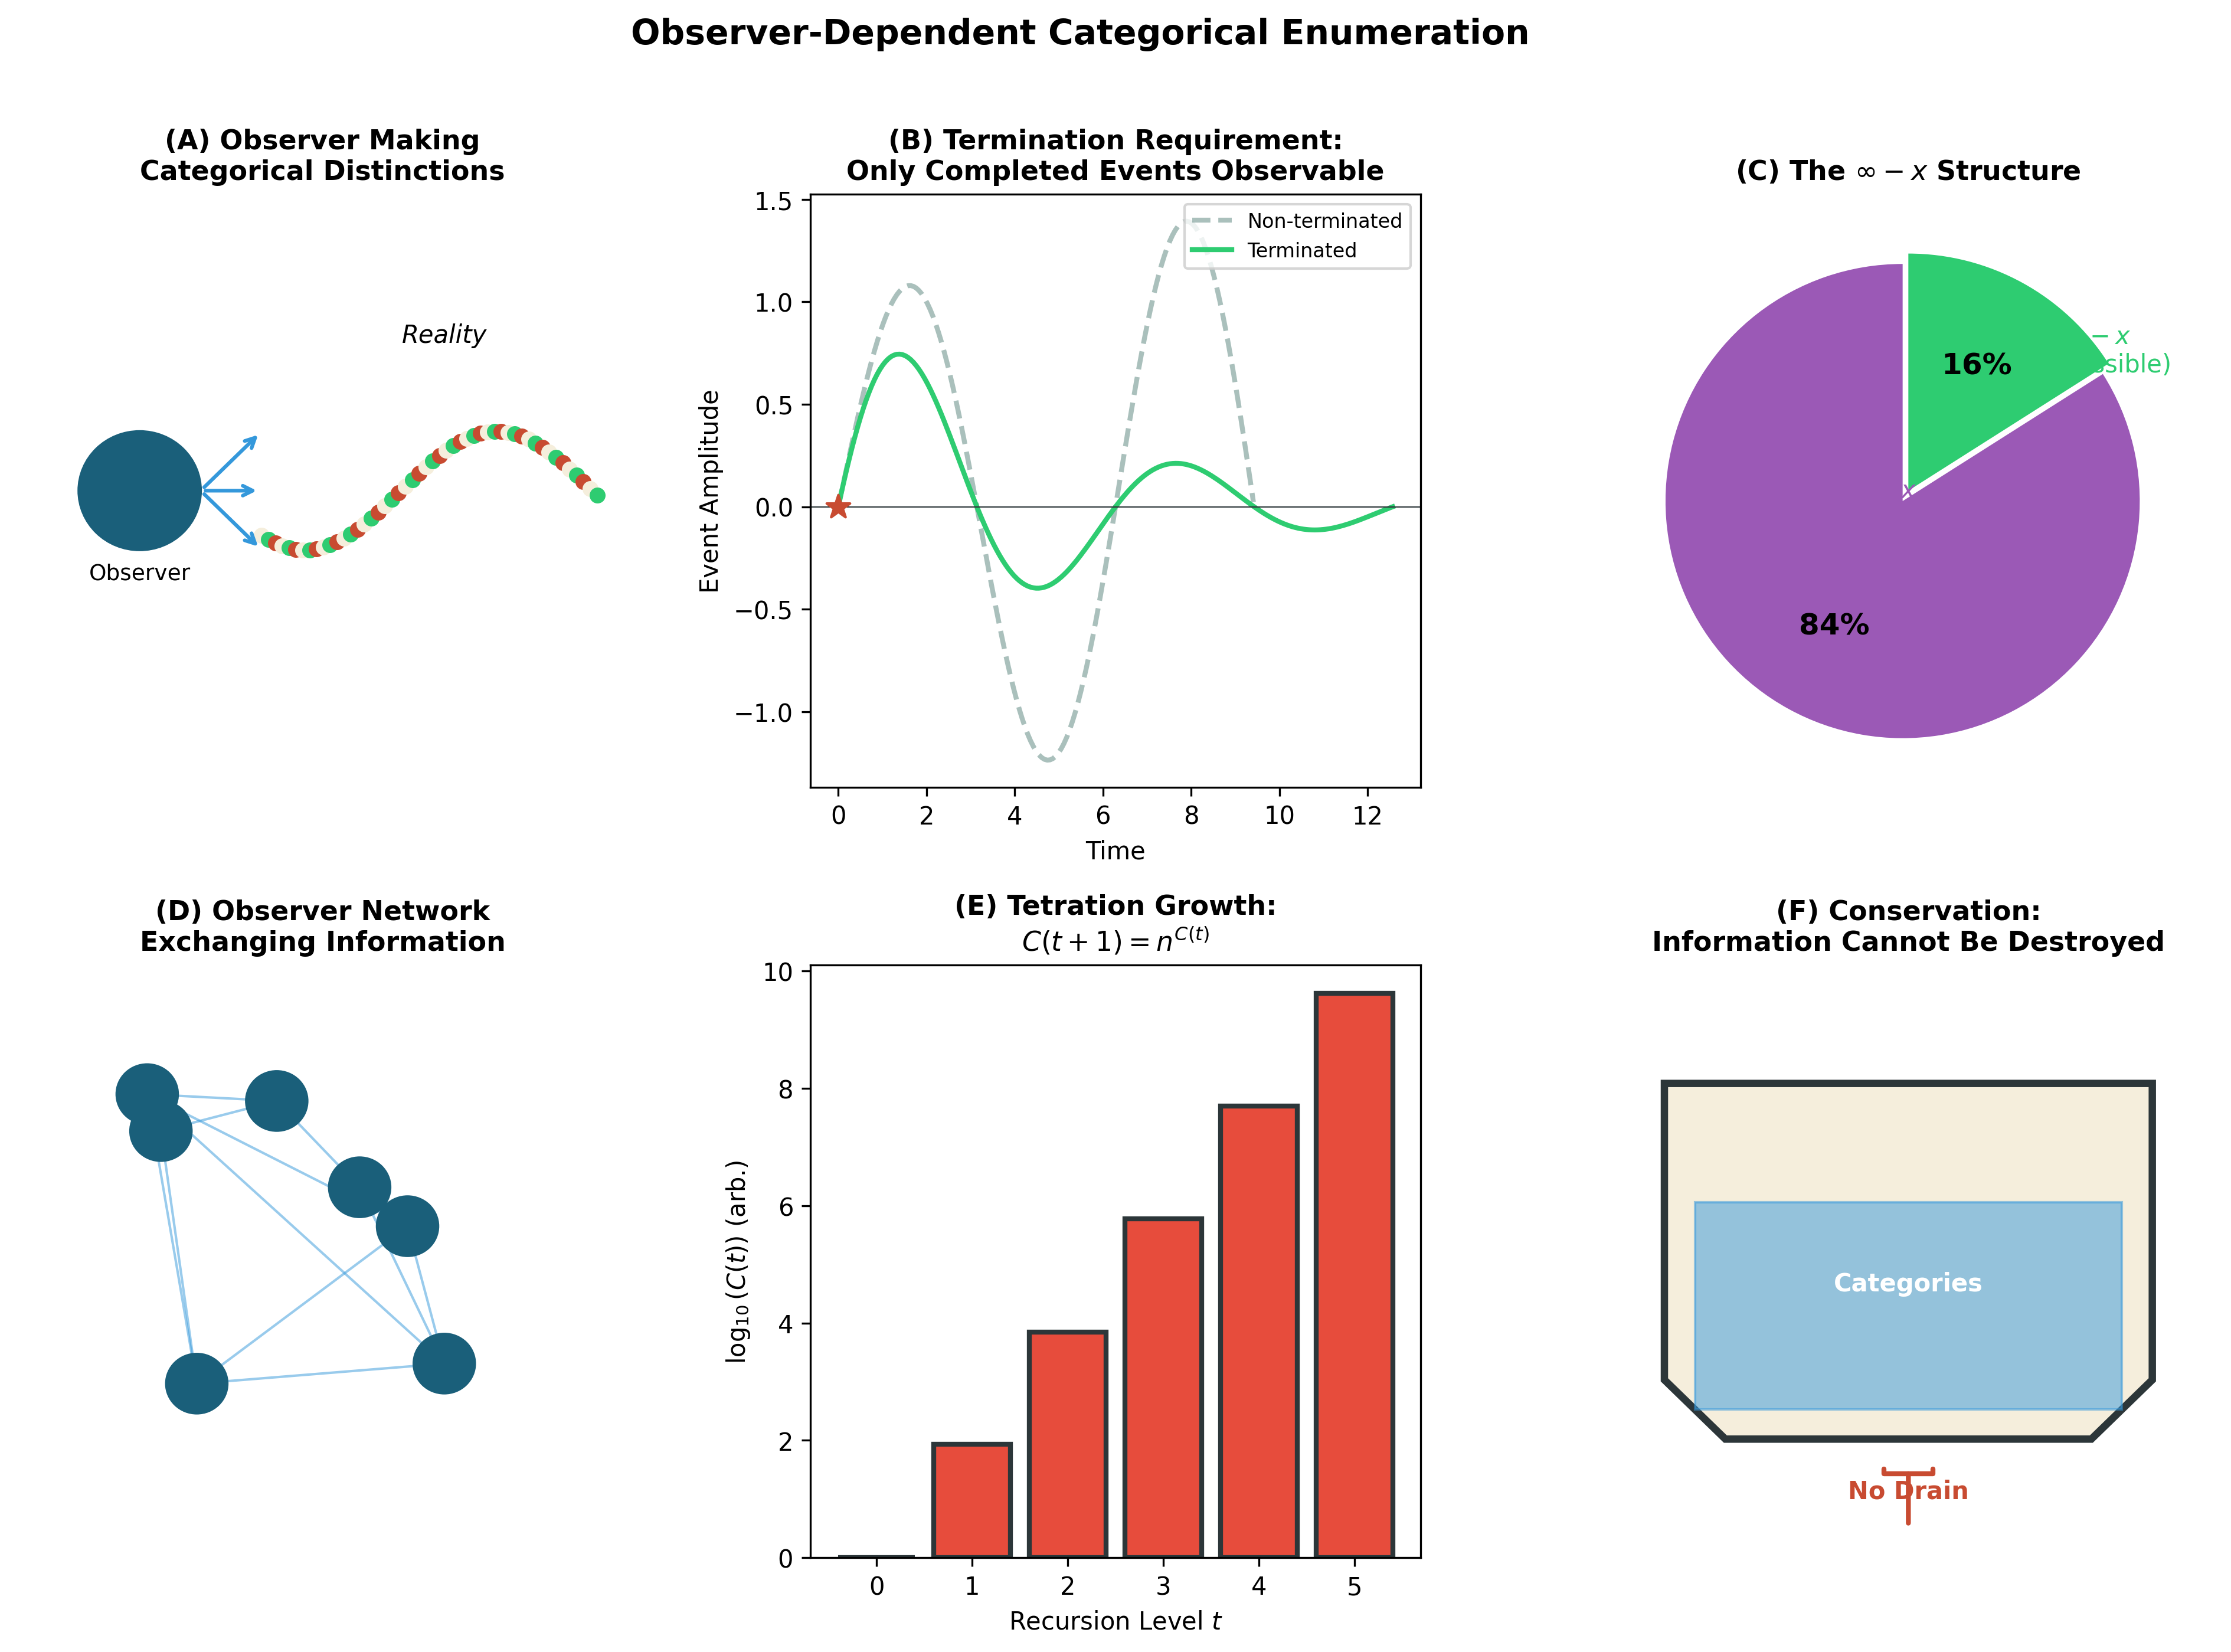
\includegraphics[width=0.48\textwidth]{observer_boundary_panel.png}
\caption{\textbf{Observer-dependent categorical enumeration and the $\infty - \times$ structure.} (\textbf{A}) Observer making categorical distinctions: observer (dark teal circle) partitions reality (wavy multicolored line) into discrete categories (colored dots). Observation $=$ categorization. (\textbf{B}) Termination requirement: only completed events are observable. Non-terminated events (gray dashed curve) have indefinite amplitude; terminated events (green solid curve) have definite outcomes. Only the latter can be measured (marked with X at $t \approx 4$ and $t \approx 10$). (\textbf{C}) The $\infty - \times$ structure: pie chart showing 84\% of reality is inaccessible ($\infty$, purple) while only 16\% is observable ($\times$, green, labeled ``visible''). This reflects the finite/infinite partition. (\textbf{D}) Observer network exchanging information: multiple observers (dark teal circles) connected by information channels (light blue lines) collectively enumerate categories. (\textbf{E}) Tetration growth: category count grows as $C(t+1) = n^{C(t)}$ (tetration), shown as red bars increasing exponentially on log scale. Recursion level $t$ on horizontal axis. (\textbf{F}) Conservation: information cannot be destroyed. Categories (blue box labeled ``Categories'') accumulate irreversibly. There is ``No Drain'' (red text)—once created, categorical information persists forever.}
\label{fig:observer_enumeration}
\end{figure*}

\begin{figure*}[t]
\centering
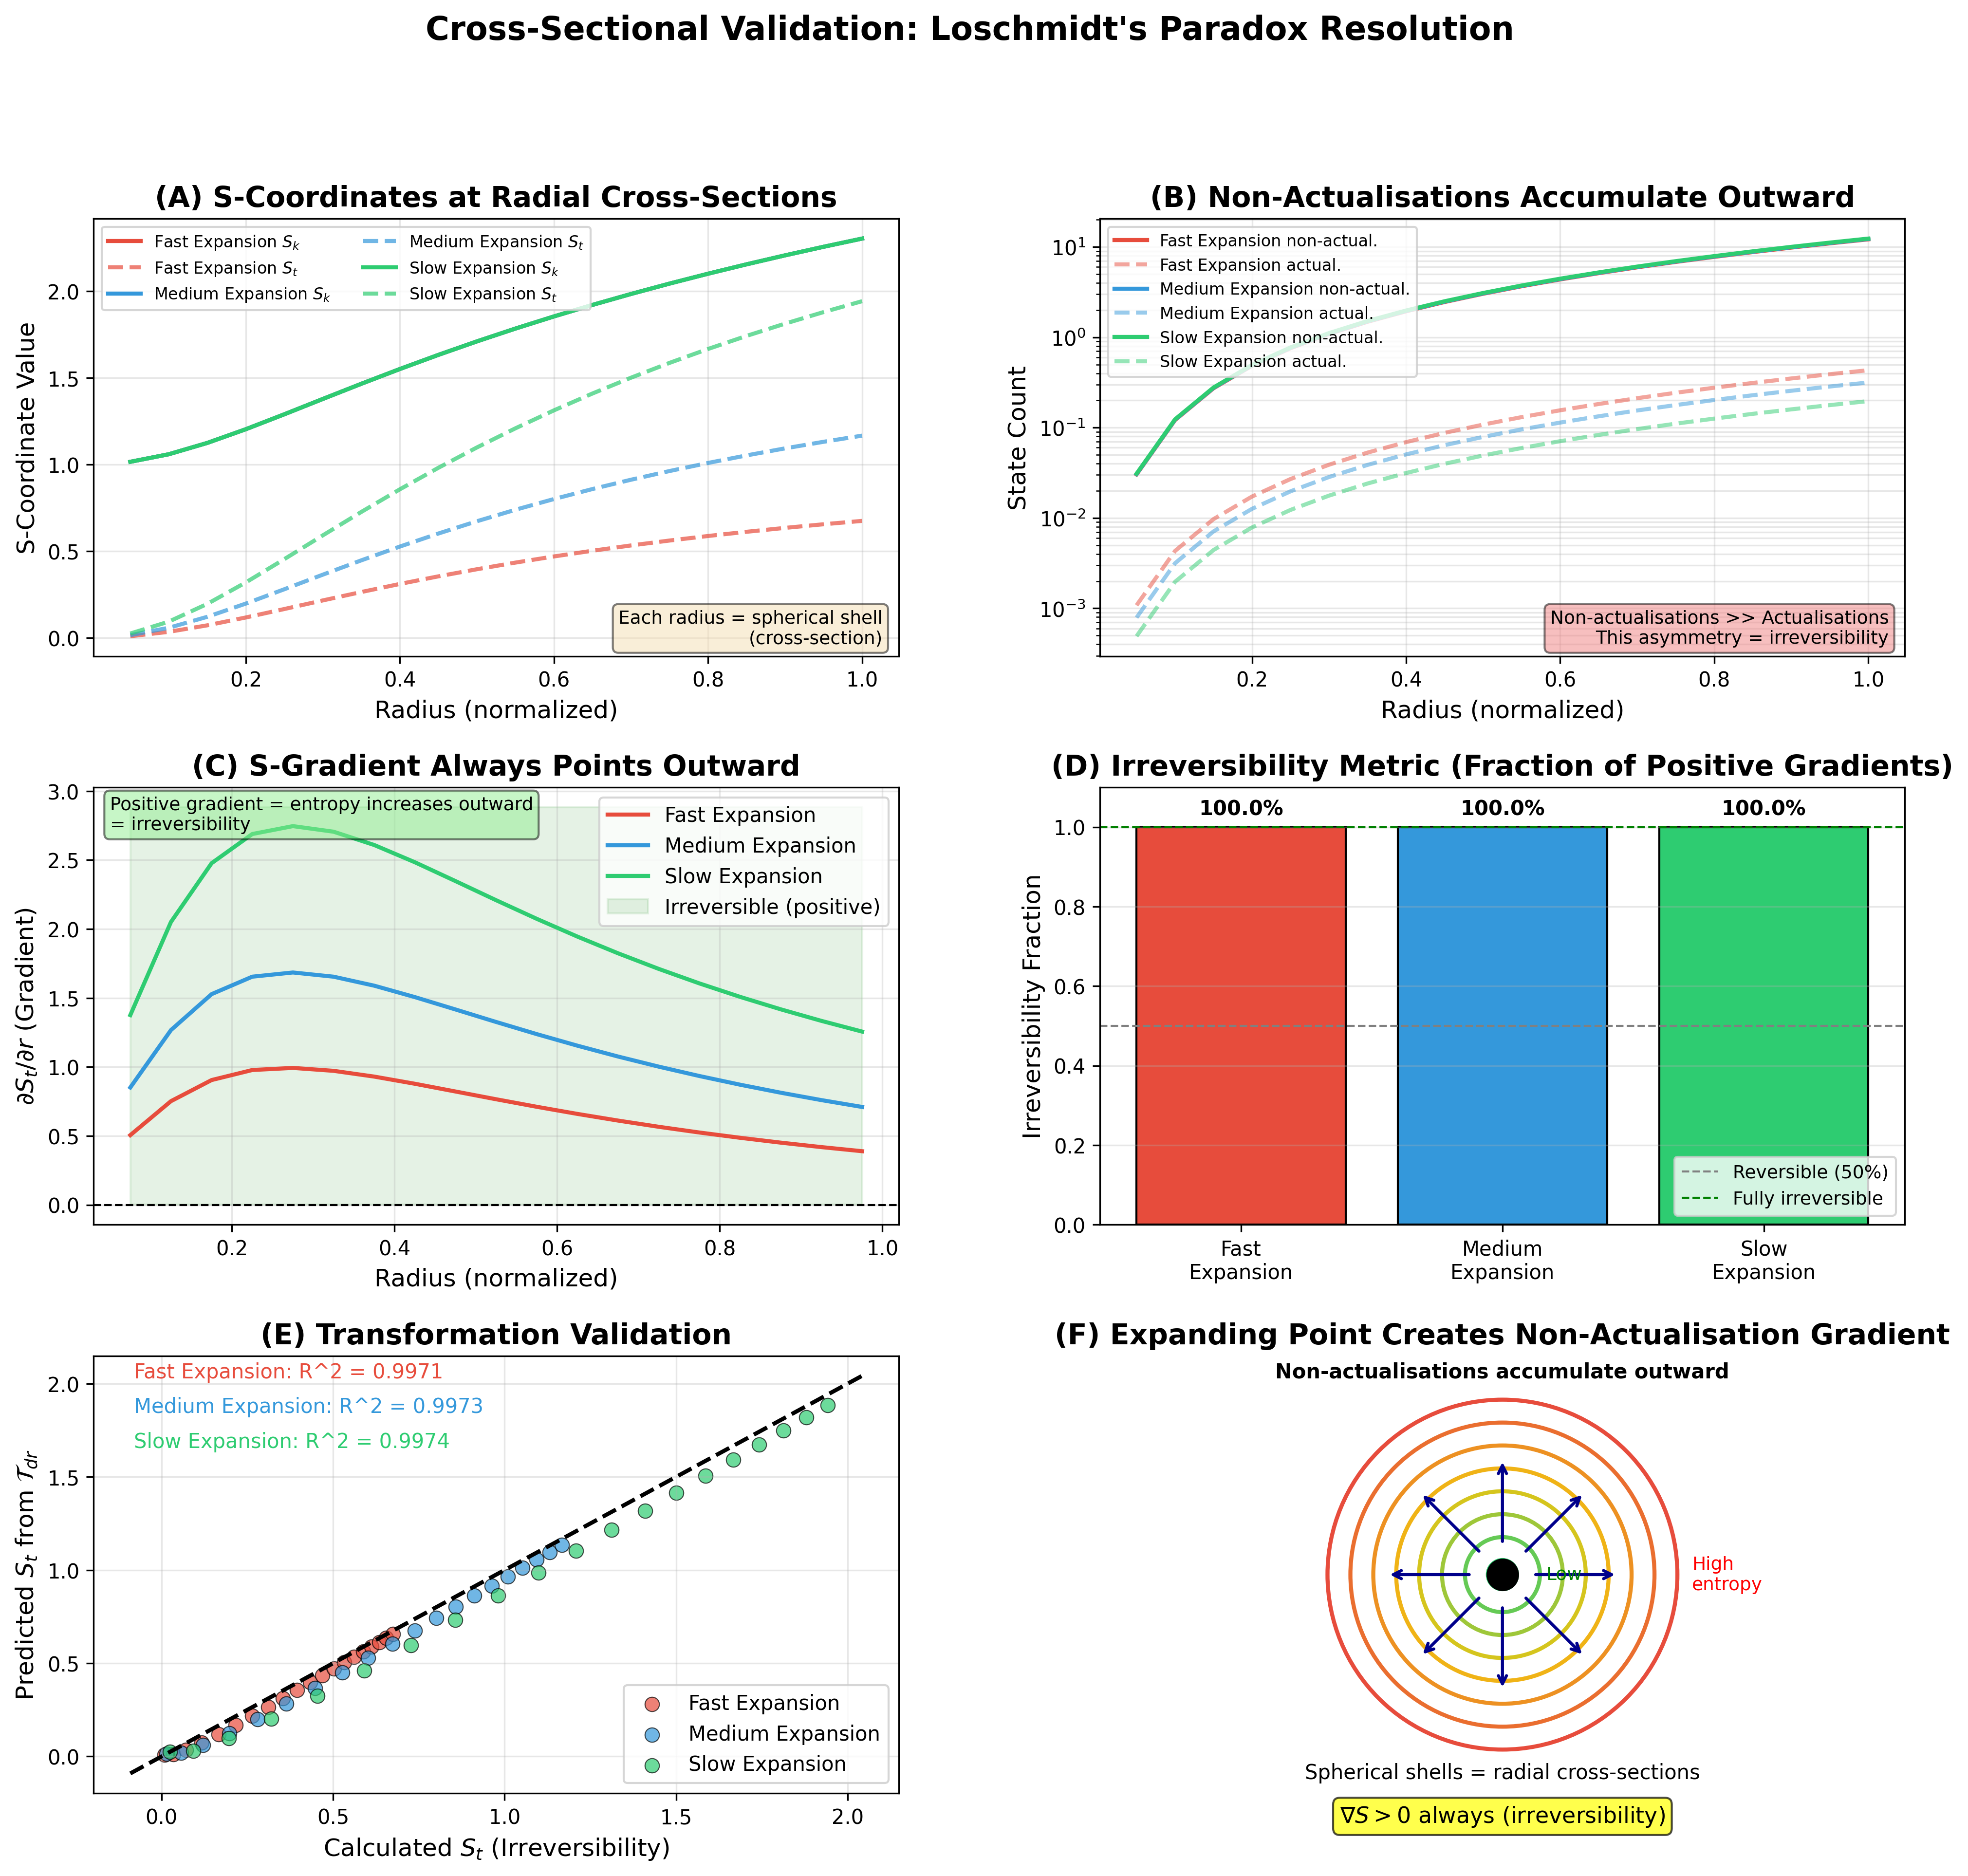
\includegraphics[width=0.95\textwidth]{panel_loschmidt_cross_sectional_validation.png}
\caption{\textbf{Cross-sectional validation of Loschmidt's paradox resolution through radial $S$-coordinate analysis.} (\textbf{A}) $S$-coordinates at radial cross-sections: temporal entropy $S_t$ (solid lines) and knowledge entropy $S_k$ (dashed lines) versus normalized radius for three expansion rates: fast (red/pink), medium (blue/cyan), slow (green/light green). Each radius corresponds to a spherical shell (cross-section). All entropies increase with radius, indicating outward entropy flow. (\textbf{B}) Non-actualizations accumulate outward: actualized states (solid lines, fast/medium/slow in red/blue/green) grow slowly, while non-actualized states (dashed lines) grow exponentially (log scale, $10^{-3}$ to $10^1$). Non-actualizations $\gg$ actualizations at all radii—this asymmetry $=$ irreversibility. (\textbf{C}) $S$-gradient always points outward: $\partial S_t/\partial r$ (vertical axis) versus normalized radius for three expansion rates (red/blue/green curves). All gradients are positive (green shaded region labeled ``Irreversible (positive)''), confirming entropy increases outward $=$ irreversibility. (\textbf{D}) Irreversibility metric (fraction of positive gradients): all three expansion rates show 100.0\% positive gradients (red/blue/green bars reaching 1.0). Reversible threshold at 50\% (magenta dashed line) and fully irreversible at 100\% (green dashed line). All cases are fully irreversible. (\textbf{E}) Transformation validation: predicted $S_t$ from transformation operator $T_{S_t}$ (vertical axis) versus calculated $S_t$ from irreversibility metric (horizontal axis) for three expansion rates (red/blue/green dots). Perfect agreement: $R^2 = 0.9971$ (fast), $0.9973$ (medium), $0.9974$ (slow). Black dashed line shows ideal $1:1$ correspondence. (\textbf{F}) Expanding point creates non-actualization gradient: polar plot showing concentric shells (red to yellow, high to low entropy) radiating from central black dot. Blue arrows indicate outward entropy gradient. Spherical shells $=$ radial cross-sections. Yellow box: ``$\nabla S > 0$ always (irreversibility).''}
\label{fig:loschmidt_validation}
\end{figure*}

\begin{figure*}[t]
\centering

\includegraphics[width=0.95\textwidth]{panel_aperture_selectivity.png}
\caption{\textbf{Partition boundaries function as categorical apertures with selectivity-dependent entropy production.} (\textbf{A}) Selection function $\sigma(\omega)$: pass or block. Incoming configurations (arrows from left) encounter aperture (gray vertical bar, partition boundary). Configurations aligned with aperture pass through ($\sigma(\omega) = 1$, green arrows labeled ``pass''), while misaligned configurations are blocked ($\sigma(\omega) = 0$, red arrows with X labeled ``blocked''). (\textbf{B}) Aperture potential: $\Phi = -kT \ln(s)$. Categorical potential (vertical axis) versus selectivity $s = \Omega_{\text{pass}}/\Omega_{\text{total}}$ (horizontal axis, 0 to 1). Blue curve shows potential diverging to $\infty$ as $s \to 0$ (red dot labeled ``$s = 0$: High selectivity, $\Phi \to \infty$'') and vanishing at $s = 1$ (green dot labeled ``$s = 1$: No selectivity, $\Phi = 0$''). Blue shaded region indicates accessible parameter space. (\textbf{C}) Entropy from selectivity: higher selectivity $\to$ more entropy. Entropy production $\Delta S/k_B = \ln(1/s) = -\ln s$ (vertical axis) shown as colored bars for four selectivity values: $s = 0.9$ (green, weak, $\Delta S \approx 0.1$), $s = 0.5$ (yellow, medium, $\Delta S \approx 0.7$), $s = 0.1$ (orange, strong, $\Delta S \approx 2.3$), $s = 0.01$ (red, very strong, $\Delta S \approx 4.6$). Formula boxed: $\Delta S = k_B \ln(1/s) = -k_B \ln s$. (\textbf{D}) Aperture as energy barrier: selectivity creates entropy. Potential energy (vertical axis) versus reaction coordinate (horizontal axis) shows barrier profile (red curve). Particle (blue dot) at left has probability $s$ to pass (green arrow labeled ``Pass (prob. $s$)'') and probability $1-s$ to be blocked (red arrow labeled ``Block (prob. $1-s$)''). Barrier height $\Phi = -kT \ln(s)$ (black arrow). Pink shaded region indicates blocked configurations. Boxed text: ``Aperture = Categorical Barrier. Blocked states $\to$ Non-actualisations.''}
\label{fig:aperture_selectivity}
\end{figure*}

\begin{figure*}[t]
\centering

\includegraphics[width=0.95\textwidth]{topology_categories_panel.png}
\caption{\textbf{Topology of categorical spaces: partial order, $S$-space structure, and completion dynamics.} (\textbf{A}) Partial order (completion precedence): directed acyclic graph showing temporal ordering of category completion. Nodes (teal circles) connected by edges represent precedence relations: upper nodes must complete before lower nodes. (\textbf{B}) Tri-dimensional $S$-space: three orthogonal axes $S_t$ (temporal entropy, red), $S_k$ (knowledge entropy, green), and $S_e$ (environmental entropy, blue) span the categorical state space. Yellow dot indicates sample state. (\textbf{C}) $3^k$ branching structure: hierarchical tree with root node $C$ (dark teal) branching into three children (blue, green, red), each further branching into three grandchildren, creating $3^k$ leaves at depth $k$. (\textbf{D}) Scale ambiguity: identical structure at different levels. Two triangular subgraphs (teal nodes) at level $n$ and level $n+1$ are related by scale transformation $\Psi_n$ (red dots with arrows), demonstrating self-similarity. (\textbf{E}) Completion trajectory $\gamma(t)$ expanding: fraction completed $|\gamma(t)|/|C|$ (green curve with shaded area) increases from 0 to asymptotic limit (red dashed line labeled ``Complete'') following sigmoidal growth. (\textbf{F}) Asymptotic slowing $\dot{C}(t) \to 0$: completion rate $\dot{C}(t)$ (red curve) decreases exponentially from $\sim 0.30$ at $t = 0$ to near zero by $t = 10$. Completion time $T$ (black dotted) diverges as system approaches full completion. Red shaded area represents integrated completion.}
\label{fig:categorical_topology}
\end{figure*}

\begin{figure*}[t]
\centering

\includegraphics[width=0.95\textwidth]{system_topology_panel.png}
\caption{\textbf{System topology validation: hierarchical branching and completion dynamics.} (\textbf{A}) $3^k$ hierarchical branching: tree structure with branching factor $k = 3$ grows from root (dark teal, $k = 0$, 1 node) to level 1 (red, 3 nodes), level 2 (blue, 9 nodes), and level 3 (green, 27 nodes). (\textbf{B}) Categorical completion dynamics: completion fraction (blue curve) increases from 0 to asymptotic limit (red dashed line at 95\% threshold) over time. Blue shaded area represents completed categories. (\textbf{C}) $S$-distance between trajectories: scatter plot showing $S$-distance (vertical axis) versus trajectory length (horizontal axis). Red dashed line indicates negative correlation: longer trajectories converge (smaller $S$-distance). Colored dots represent individual trajectory pairs. (\textbf{D}) Equivalence class distribution: histogram showing class sizes (vertical axis) versus equivalence class index (horizontal axis). Purple bars indicate most classes have moderate size; red bar (class 4) shows one large equivalence class with $\sim 25$ members. (\textbf{E}) Degeneracy-richness relationship: scatter plot (green dots) with linear fit (red dashed line). Richness $R(C)$ increases with degeneracy $D(C)$, confirming that more degenerate states support greater structural richness. (\textbf{F}) Scale ambiguity (structure similarity): radar plot showing structural similarity at different scales $k = 0, 1, 2, 3, 4$ (orange polygon). All scales exhibit similar topology, confirming scale invariance.}
\label{fig:topology_validation}
\end{figure*}

\begin{figure*}[t]
\centering
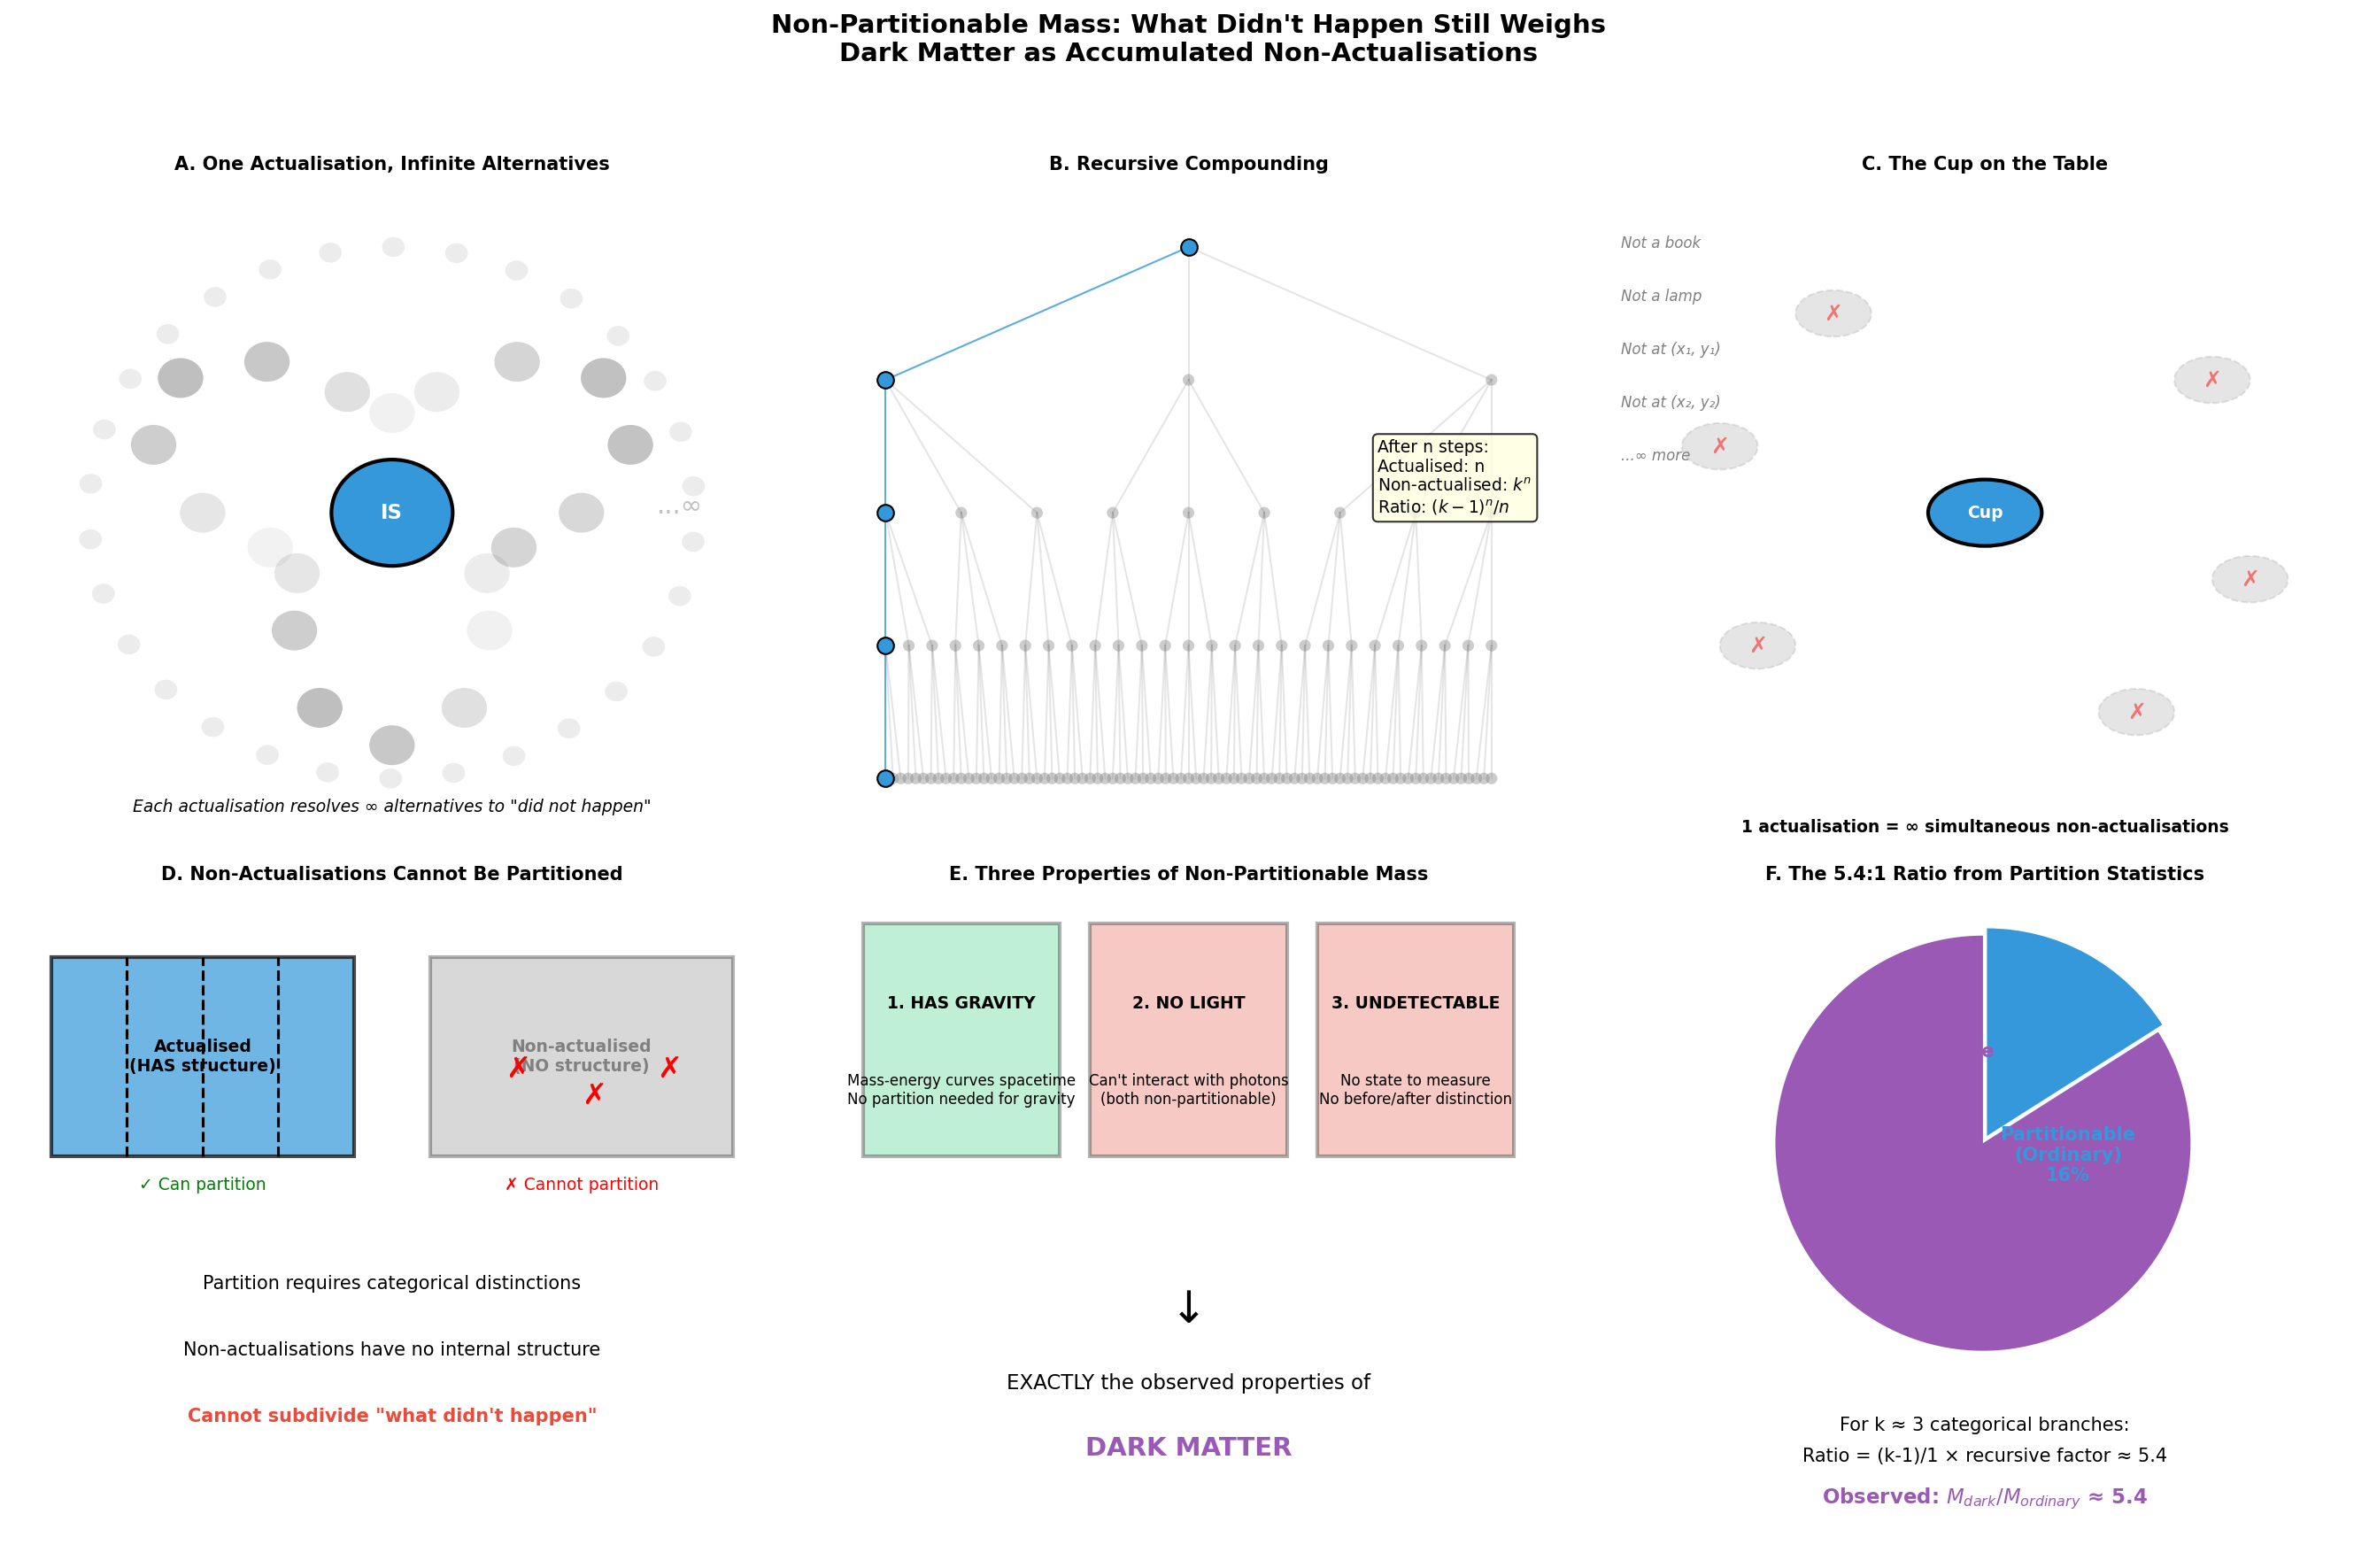
\includegraphics[width=0.95\textwidth]{recursive_compounding_panel.png}
\caption{\textbf{Non-partitionable mass: what didn't happen still weighs—dark matter as accumulated non-actualizations.} (\textbf{A}) One actualization, infinite alternatives: single actualized state (large blue circle labeled ``is'') surrounded by infinite gray circles representing non-actualized alternatives. Each actualization resolves $\infty$ alternatives to ``did not happen.'' (\textbf{B}) Recursive compounding: tree structure showing exponential growth. After $n$ steps: actualized states $= n$ (blue nodes), non-actualized states $= k^n$ (gray nodes), ratio $= (k-1)^n/n$. (\textbf{C}) The cup on the table: actualized state (blue circle labeled ``Cup'') is surrounded by infinite non-actualizations (pink circles with X): not a book, not a lamp, not at $(x_1, y_1)$, not at $(x_2, y_2)$, $\ldots$ more. 1 actualization $= \infty$ simultaneous non-actualizations. (\textbf{D}) Non-actualizations cannot be partitioned: actualized states (blue box, ``HAS structure'') can be partitioned (checkmark). Non-actualized states (gray box, ``NO structure'', X) cannot be partitioned (X). Partition requires categorical distinctions; non-actualizations have no internal structure. Cannot subdivide ``what didn't happen.'' (\textbf{E}) Three properties of non-partitionable mass: (1) \textbf{Has gravity} (green box): mass-energy curves spacetime, no partition needed for gravity. (2) \textbf{No light} (pink box): can't interact with photons (both non-partitionable). (3) \textbf{Undetectable} (red box): no state to measure, no before/after distinction. Arrow points to: ``EXACTLY the observed properties of \textbf{DARK MATTER}.'' (\textbf{F}) The 5.4:1 ratio from partition statistics: pie chart showing 84\% non-partitionable (purple, dark matter) versus 16\% partitionable (blue, ordinary matter). For $k \sim 3$ categorical branches: ratio $\approx (k-1)/1 \times \text{recursive factor} \sim 5.4$. Observed: $M_{\text{dark}}/M_{\text{ordinary}} \approx 5.4$.}
\label{fig:dark_matter_mechanism}
\end{figure*}


\begin{figure*}[t]
\centering
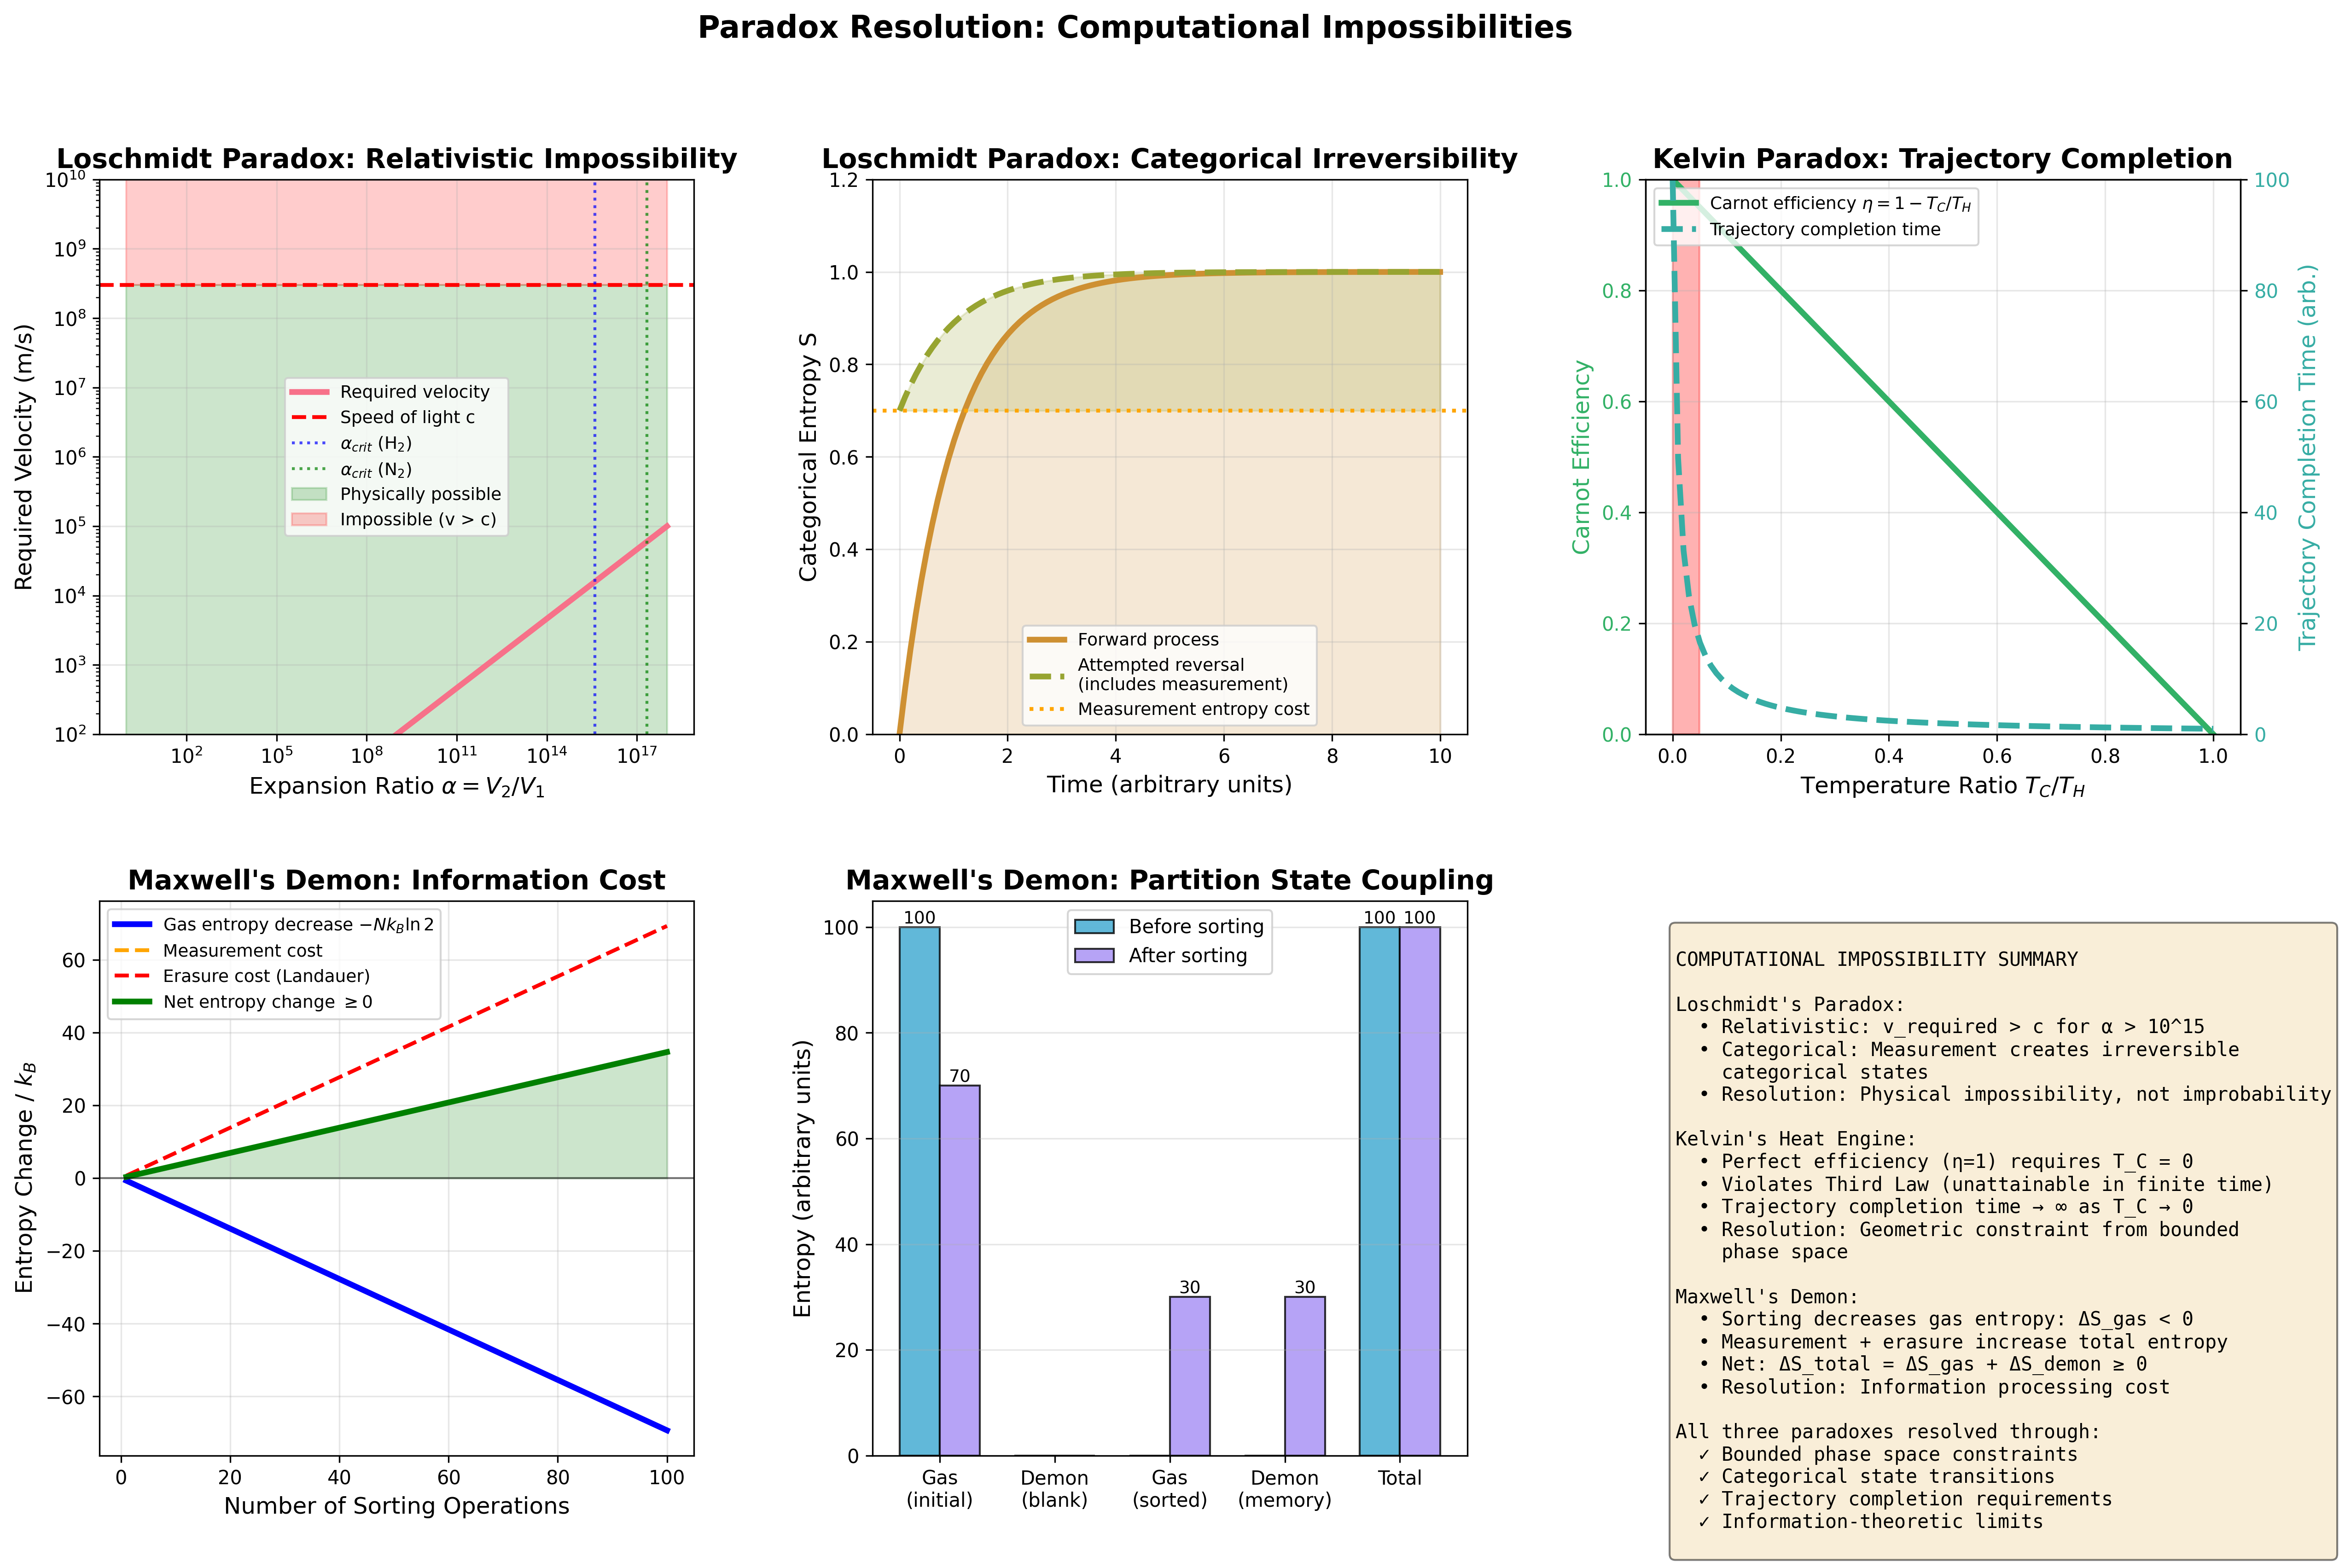
\includegraphics[width=0.95\textwidth]{paradox_resolutions.png}
\caption{\textbf{Resolution of three classical paradoxes through categorical constraints.} (\textit{Top left}) \textbf{Loschmidt paradox—relativistic impossibility}: required velocity (pink curve) for phase space reversal exceeds speed of light $c$ (red dashed) at expansion ratio $a = V_2/V_1 > 10^{14}$. Critical velocities for H$_2$ (purple dotted) and N$_2$ (green dotted) mark molecular-specific thresholds. Green shaded region: physically possible; red shaded region: impossible ($v > c$). (\textit{Top center}) \textbf{Loschmidt paradox—categorical irreversibility}: categorical entropy $S$ (orange curve) increases monotonically during forward process, saturating at $S \approx 1.0$. Attempted reversal (green dashed) including measurement creates additional entropy (orange shaded region). Measurement entropy cost (yellow dotted) prevents return to $S = 0$. (\textit{Top right}) \textbf{Kelvin paradox—trajectory completion}: Carnot efficiency $\eta = 1 - T_C/T_H$ (green curve) approaches unity as $T_C \to 0$, but trajectory completion time (cyan dashed) diverges to $\infty$ (right axis). Red shaded region: thermodynamically forbidden. (\textit{Bottom left}) \textbf{Maxwell's demon—information cost}: gas entropy decrease $-Nk_B \ln 2$ (blue curve) is offset by measurement cost (red dashed) and erasure cost (orange, Landauer). Net entropy change $\geq 0$ (green curve, shaded). (\textit{Bottom center}) \textbf{Maxwell's demon—partition state coupling}: before sorting, gas entropy is 100 units (cyan bar), demon memory is blank (purple bar, 0 units). After sorting, gas entropy decreases to 70 units, but demon memory increases to 30 units. Total entropy remains 100 units. (\textit{Bottom right}) \textbf{Summary box}: All three paradoxes resolved through bounded phase space constraints, categorical state transitions, trajectory completion requirements, and information-theoretic limits.}
\label{fig:paradox_resolution}
\end{figure*}

\begin{figure*}[t]
\centering
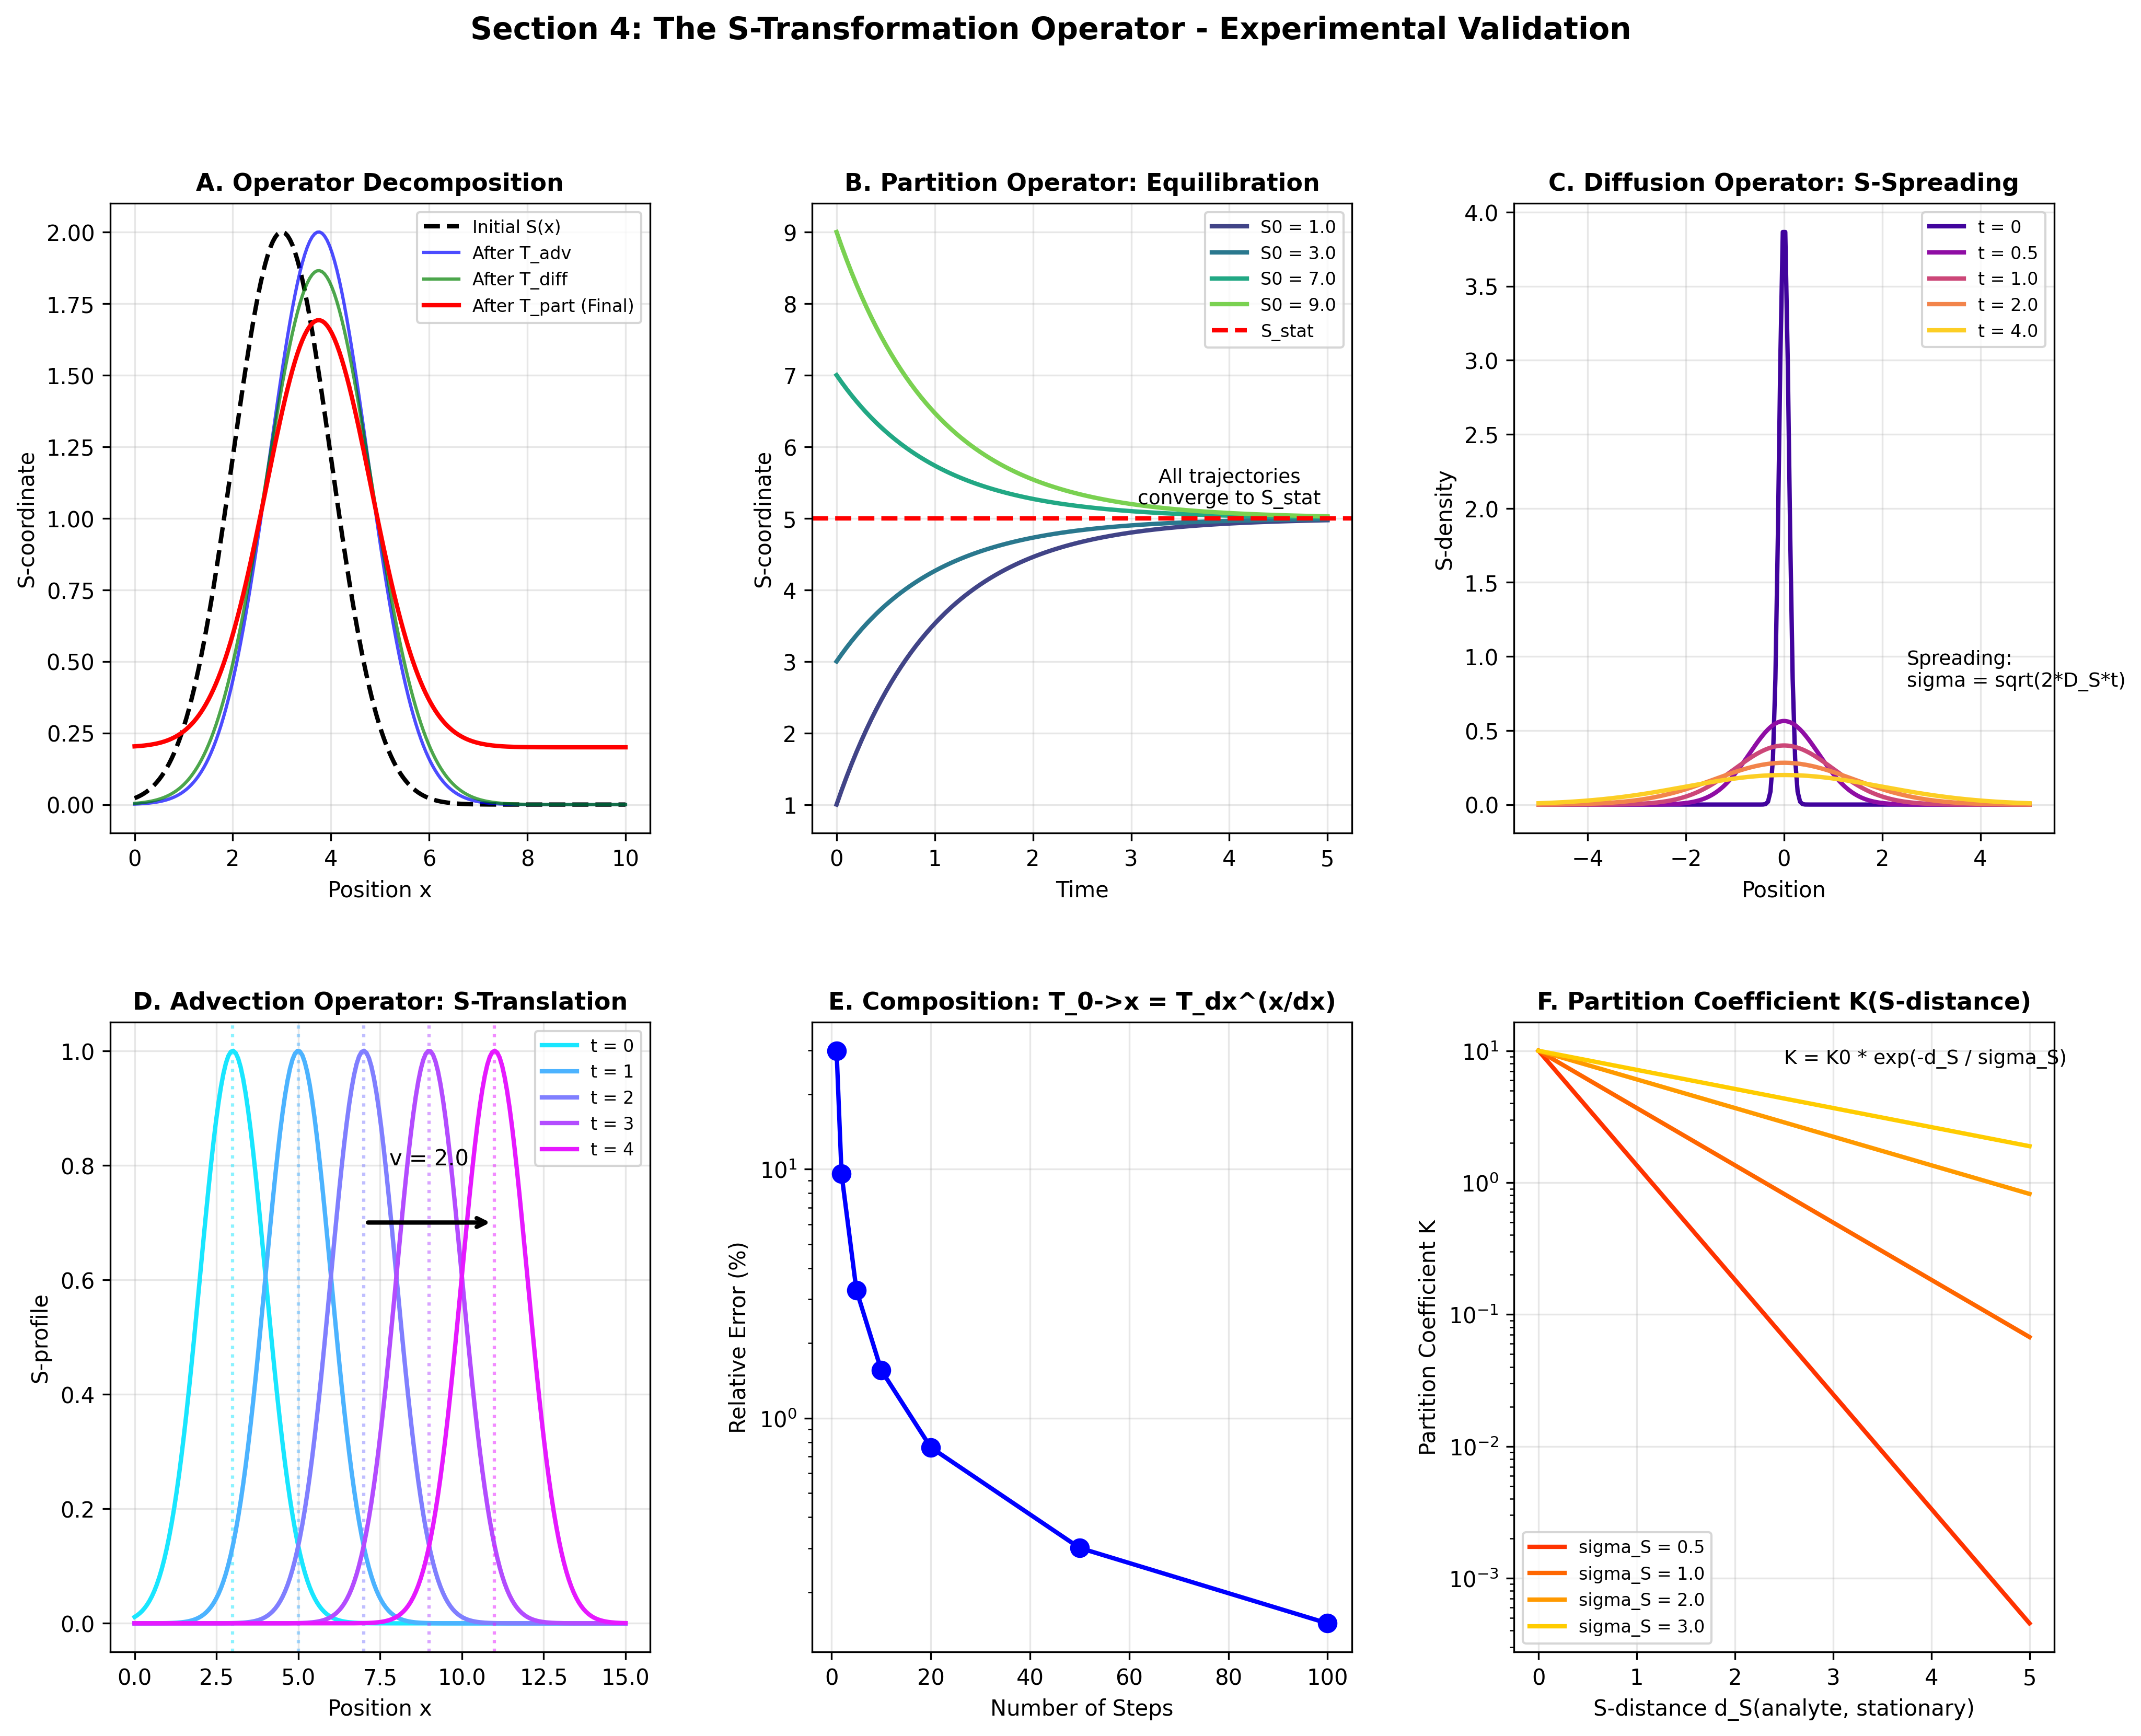
\includegraphics[width=0.95\textwidth]{panel_transformation_operator.png}
\caption{\textbf{The $S$-transformation operator: decomposition and experimental validation.} (\textbf{A}) Operator decomposition: initial $S$-profile (black dashed) undergoes advection $T_{\text{adv}}$ (blue), diffusion $T_{\text{diff}}$ (green), and partition $T_{\text{part}}$ (red, final) to reach equilibrium. (\textbf{B}) Partition operator equilibration: trajectories starting at different initial values $S_0 = 1.0, 3.0, 7.0, 9.0$ (colored curves) all converge to stationary state $S_{\text{stat}}$ (red dashed line at $S \approx 5$) over time. (\textbf{C}) Diffusion operator $S$-spreading: initial delta function (purple spike at $t = 0$) spreads according to $\sigma = \sqrt{2D_S t}$ (colored curves at $t = 0.5, 1.0, 2.0, 4.0$). (\textbf{D}) Advection operator $S$-translation: $S$-profile (colored Gaussian peaks) translates rightward with velocity $v = 2.0$ (purple arrow) at successive times $t = 0, 1, 2, 3, 4$ (cyan to magenta). (\textbf{E}) Composition: $T_{0 \to x} = T_{\text{dx}}^{(x/dx)}$. Relative error (vertical axis, log scale) decreases from $\sim 10^1\%$ at 10 steps to $< 10^{-1}\%$ at 100 steps (blue dots), validating operator composition. (\textbf{F}) Partition coefficient $K(S\text{-distance})$: exponential decay $K = K_0 \exp(-d_S/\sigma_S)$ for different spreading parameters $\sigma_S = 0.5, 1.0, 2.0, 3.0$ (red to yellow curves). Steeper decay (red) indicates stronger selectivity.}
\label{fig:s_transformation}
\end{figure*}

\begin{figure*}[t]
\centering
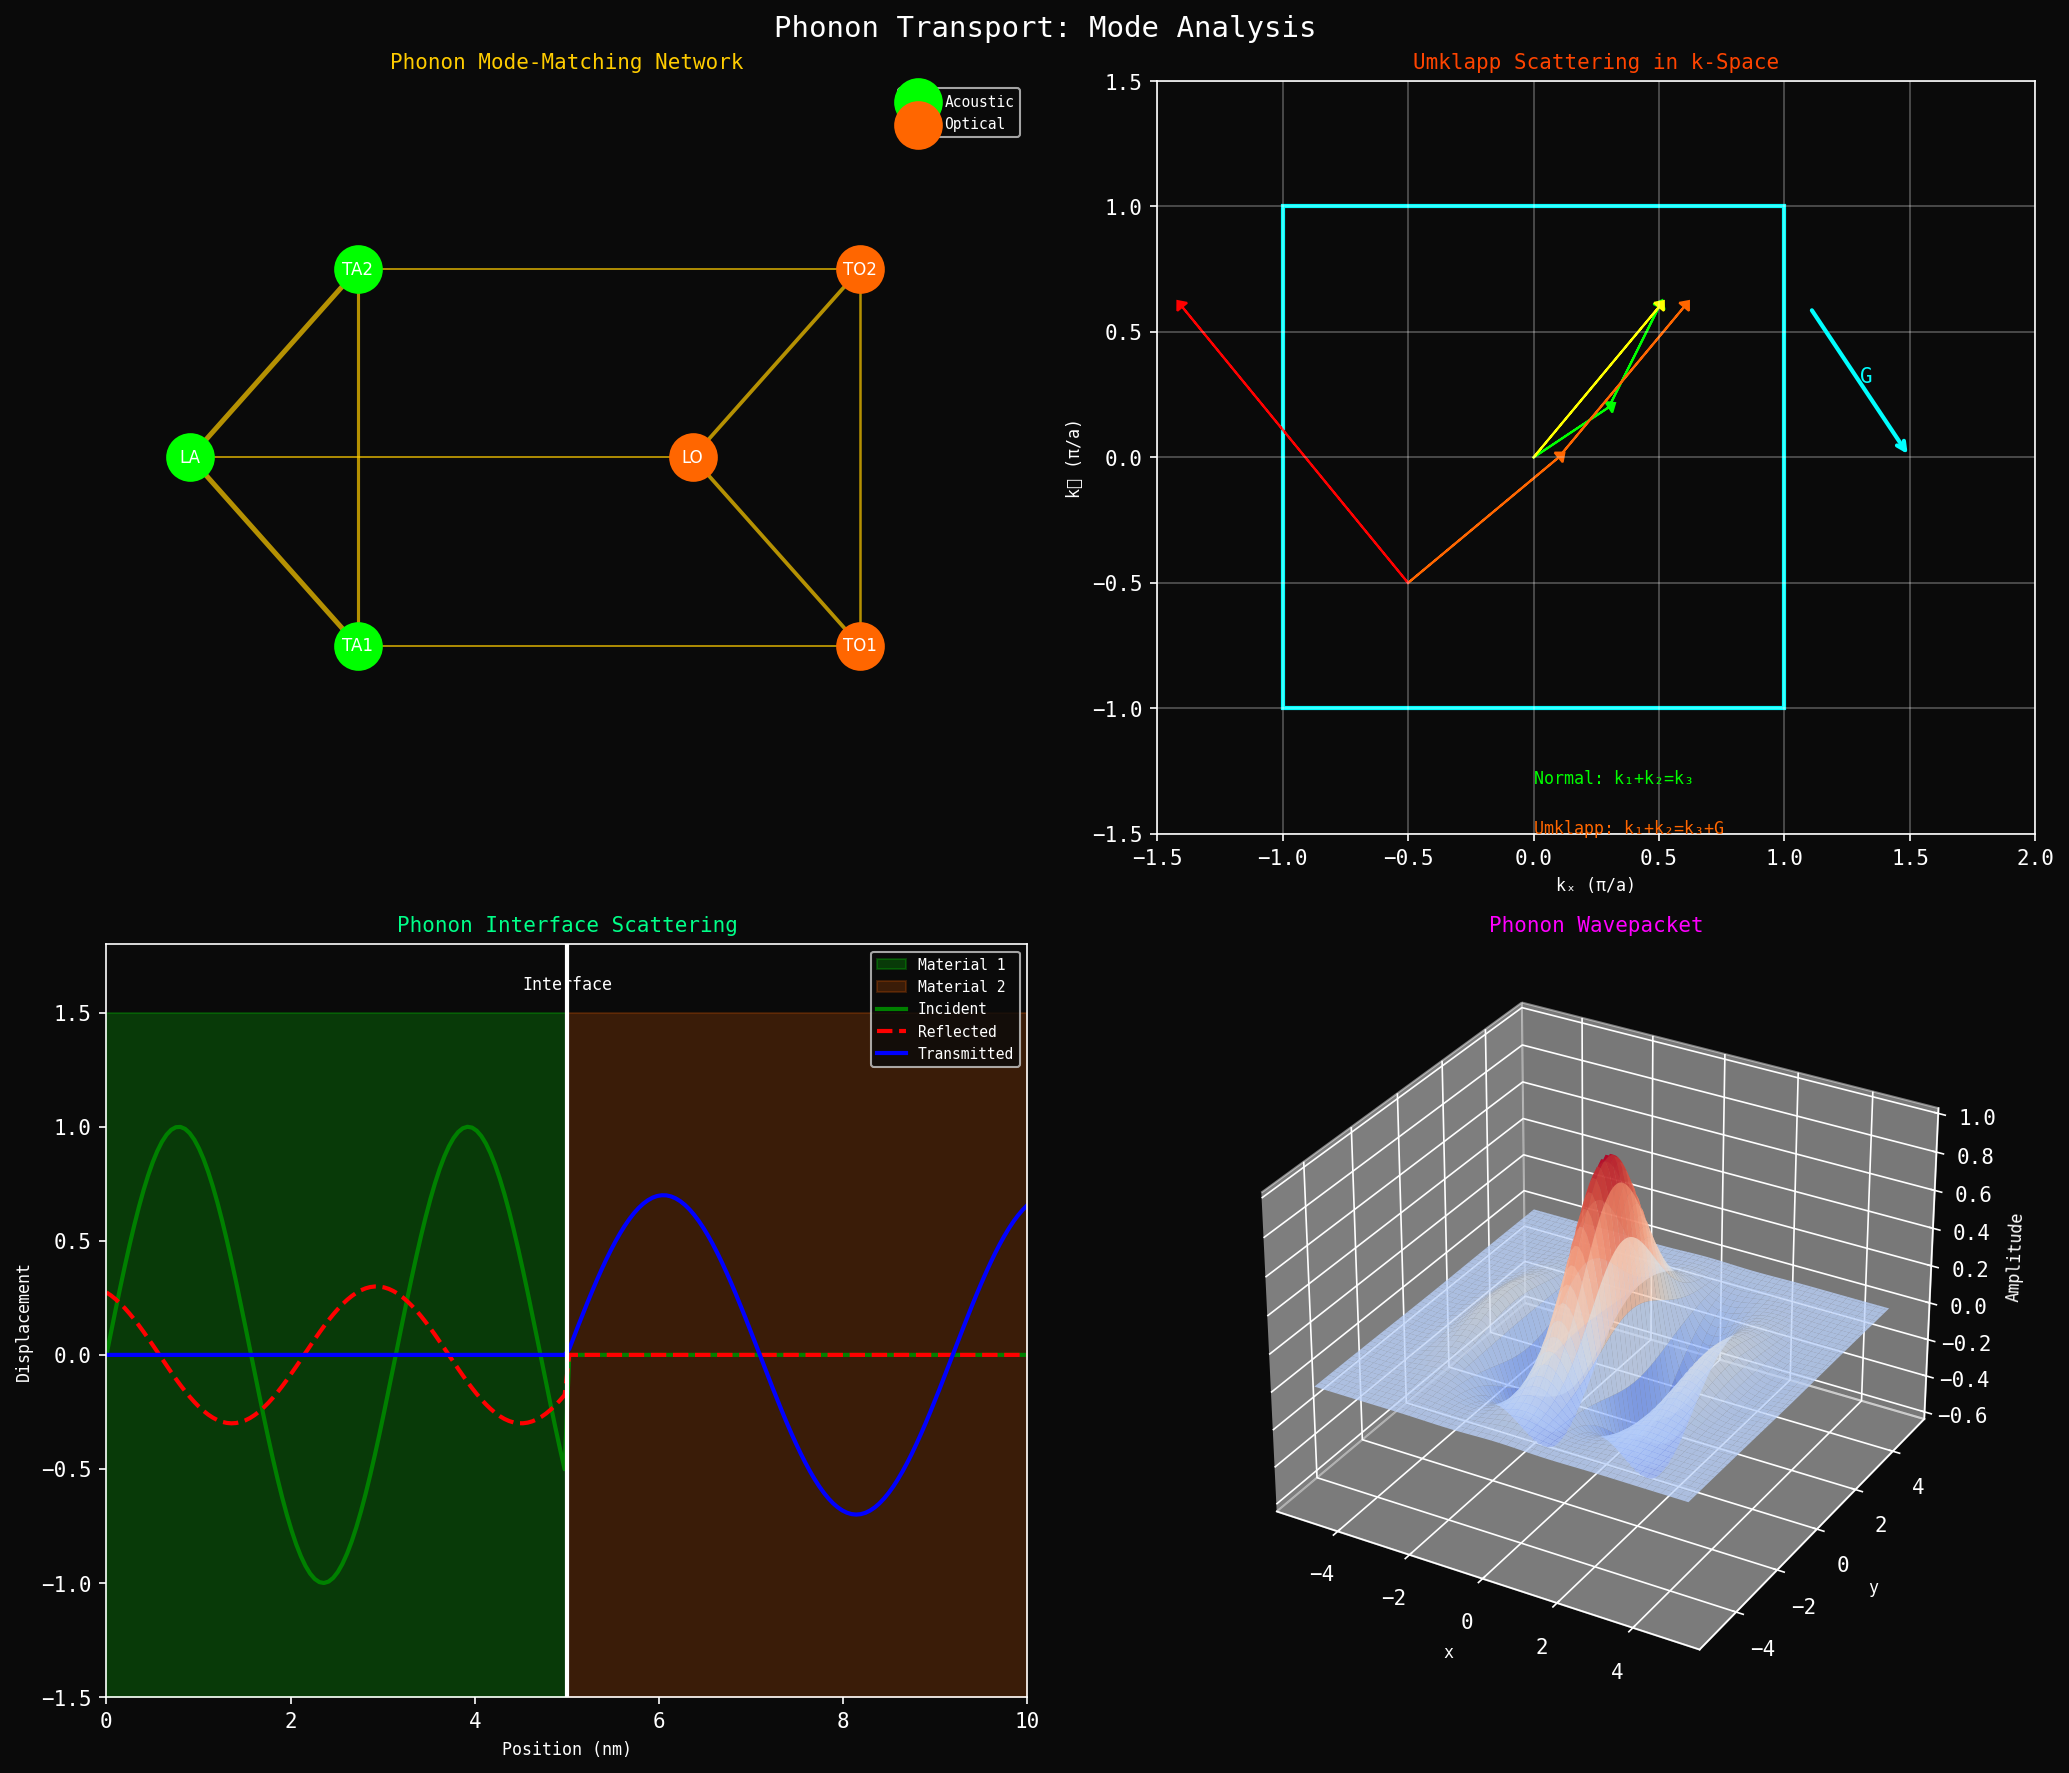
\includegraphics[width=0.95\textwidth]{panel_phonon_analysis.png}
\caption{\textbf{Phonon transport: mode analysis across acoustic and optical branches.} (\textit{Top left}) \textbf{Phonon mode-matching network}: acoustic modes (green circles labeled TA1, TA2, LA) and optical modes (orange circles labeled TO1, TO2) form bipartite network connected by coupling edges (gold lines). (\textit{Top right}) \textbf{Umklapp scattering in $k$-space}: first Brillouin zone (cyan square) showing normal scattering (green arrow, $\vec{k}_1 + \vec{k}_2 = \vec{k}_3$) versus umklapp scattering (red and yellow arrows, $\vec{k}_1 + \vec{k}_2 = \vec{k}_3 + \vec{G}$ where $\vec{G}$ is reciprocal lattice vector). (\textit{Bottom left}) \textbf{Phonon interface scattering}: incident wave (green region) encounters interface between Material 1 and Material 2 (brown region). Reflected (blue curve) and transmitted (orange curve) components shown. Displacement oscillates with position. (\textit{Bottom right}) \textbf{Phonon wavepacket}: 3D visualization showing spatial localization of phonon amplitude. Red peak (positive displacement) and blue trough (negative displacement) form localized wavepacket propagating through crystal.}
\label{fig:phonon_transport}
\end{figure*}

\begin{figure*}[t]
\centering
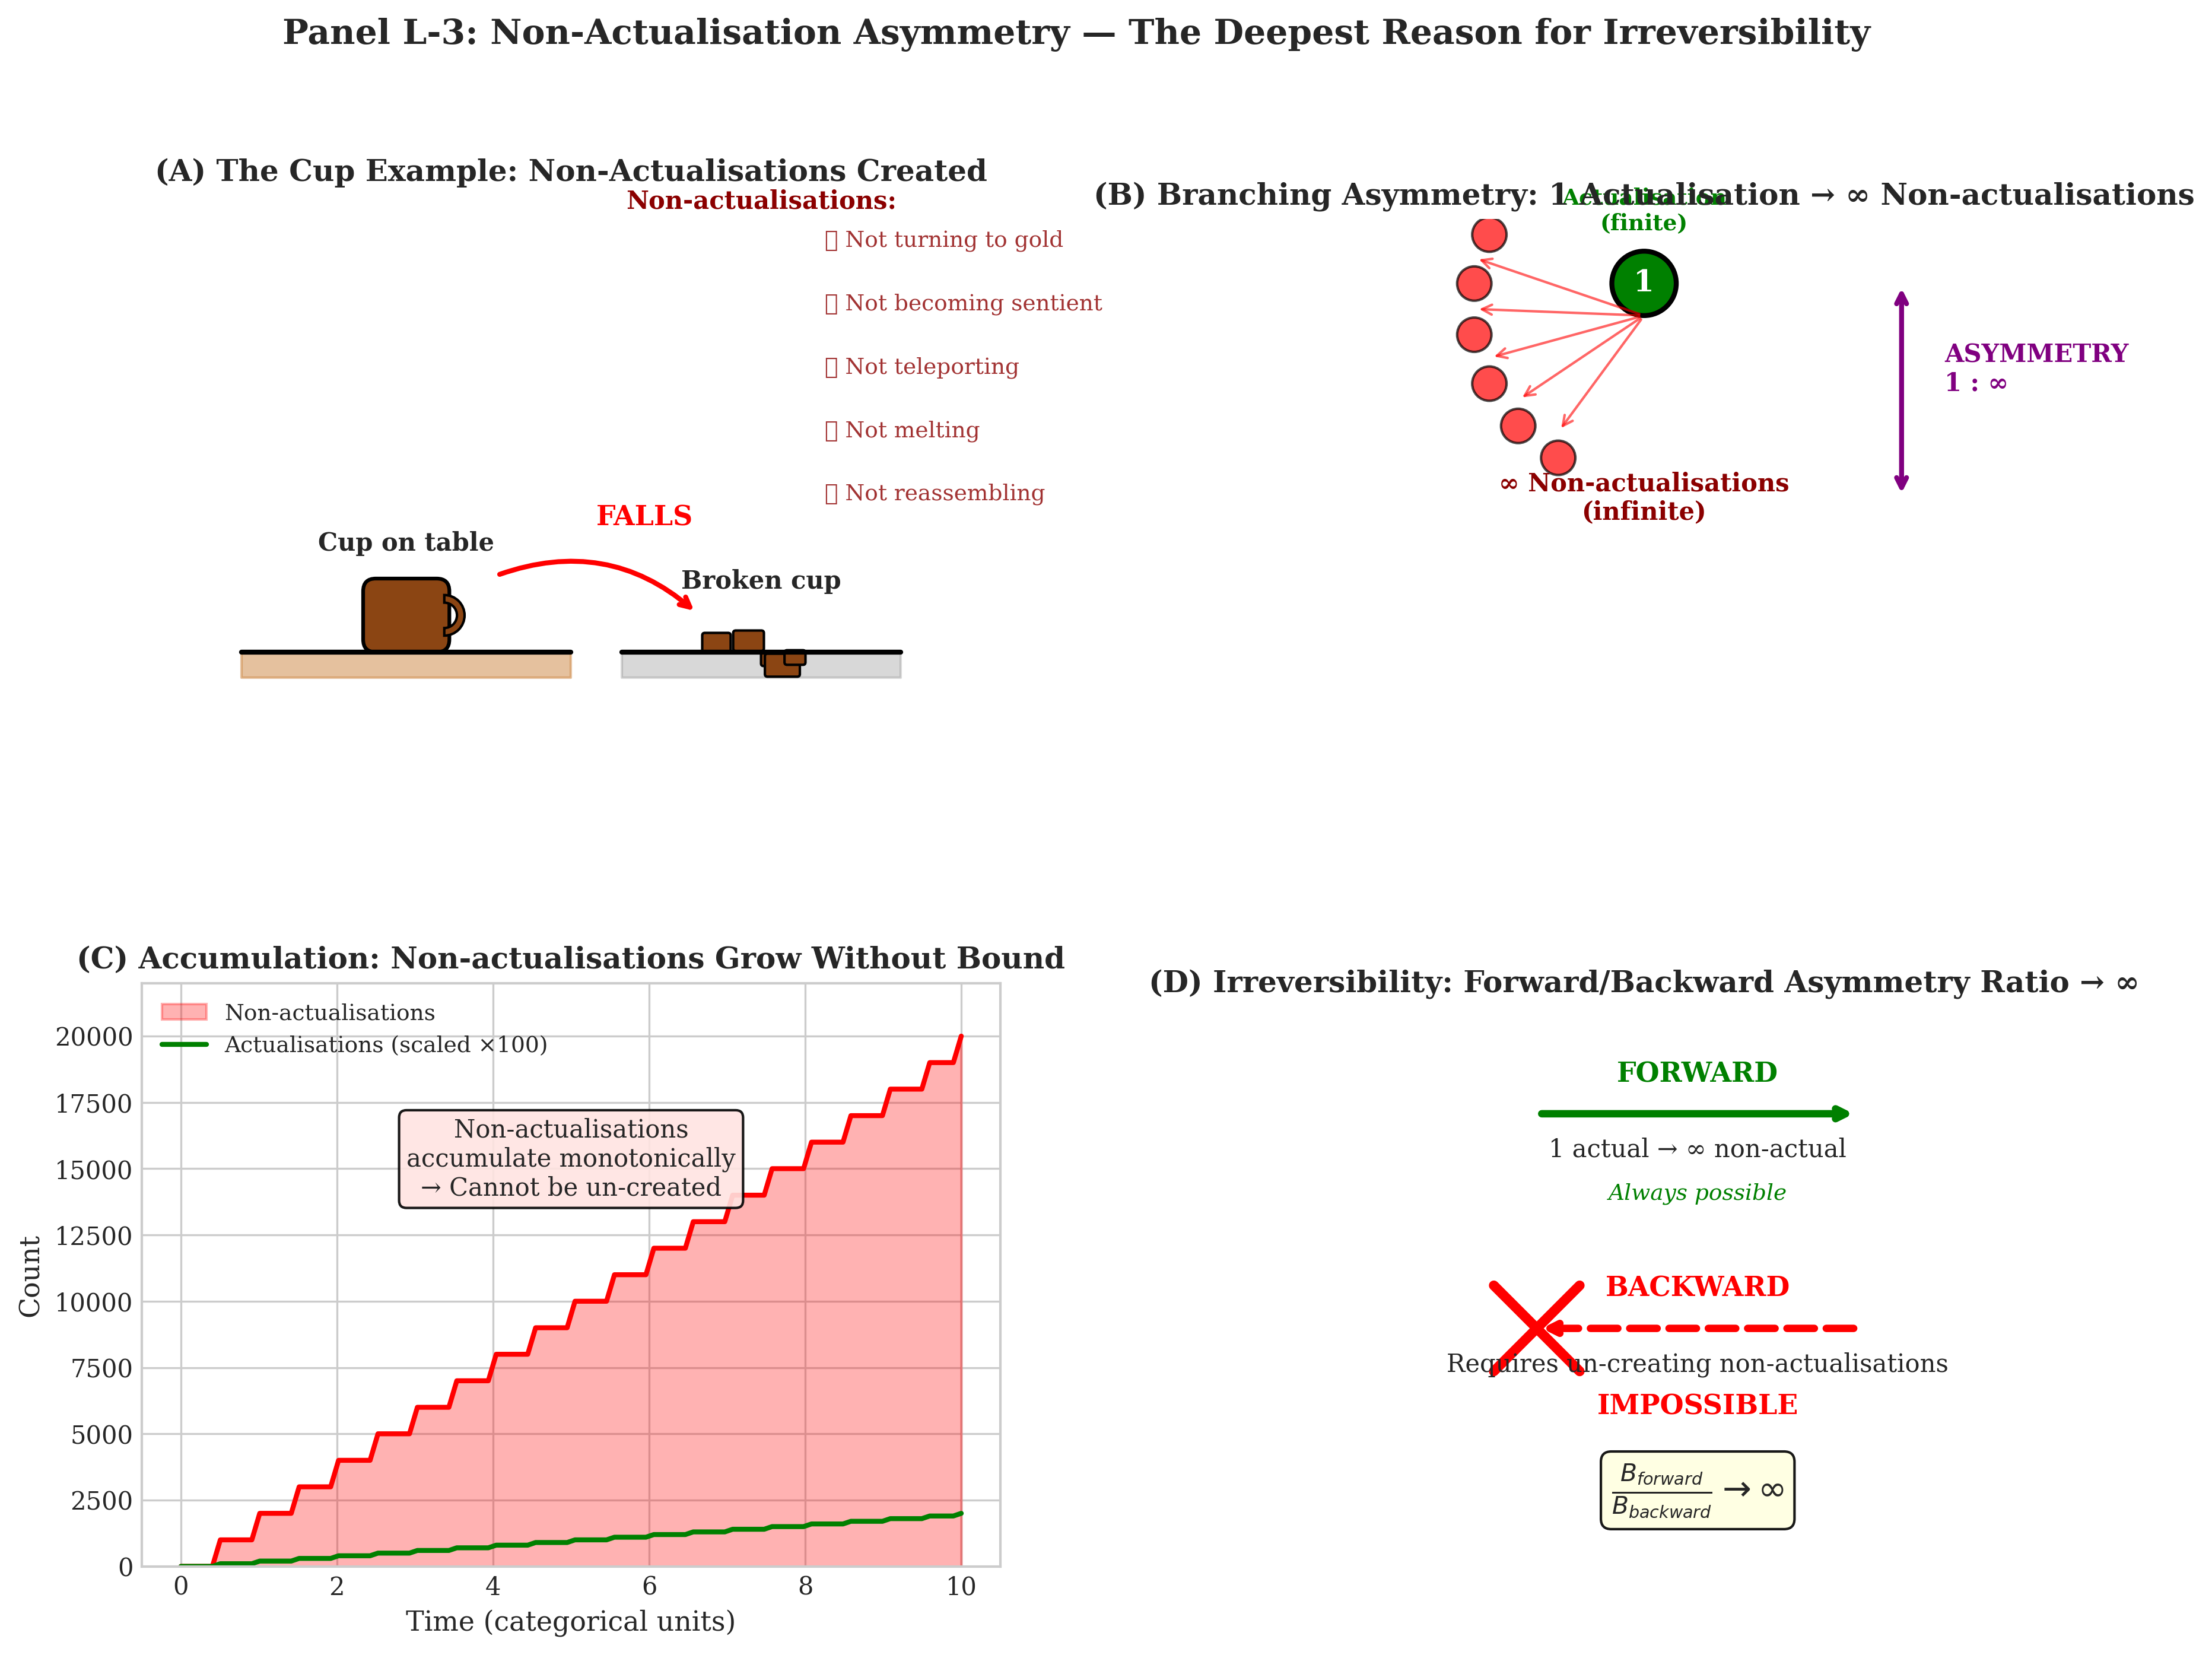
\includegraphics[width=0.95\textwidth]{panel_non_actualisation.png}
\caption{\textbf{Non-actualization asymmetry provides the deepest reason for irreversibility.} (\textbf{A}) The cup example: when a cup falls from table to broken state, a single actualization (cup breaks) creates infinite non-actualizations: $\Box$ not turning to gold, $\Box$ not becoming sentient, $\Box$ not teleporting, $\Box$ not melting, $\Box$ not reassembling, and infinitely many more. Each actualization generates $\infty$ resolved non-possibilities. (\textbf{B}) Branching asymmetry: one actualization (green circle labeled ``1'') leads to $\infty$ non-actualizations (red circles, infinite). The asymmetry ratio is $1:\infty$, indicated by purple double arrow. (\textbf{C}) Accumulation: non-actualizations grow without bound. Red shaded area shows non-actualizations accumulating monotonically over time (reaching $\sim 20{,}000$ by $t = 10$), while actualizations (green line, scaled $\times 100$) grow slowly. Non-actualizations accumulate monotonically and cannot be un-created. (\textbf{D}) Irreversibility: forward/backward asymmetry ratio $\to \infty$. \textbf{Forward} (green arrow): 1 actual $\to \infty$ non-actual is always possible. \textbf{Backward} (red crossed arrow): requires un-creating non-actualizations, which is \textbf{impossible}. The ratio $B_{\text{forward}}/B_{\text{backward}} \to \infty$ establishes absolute irreversibility.}
\label{fig:non_actualization}
\end{figure*}

\begin{figure*}[t]
\centering
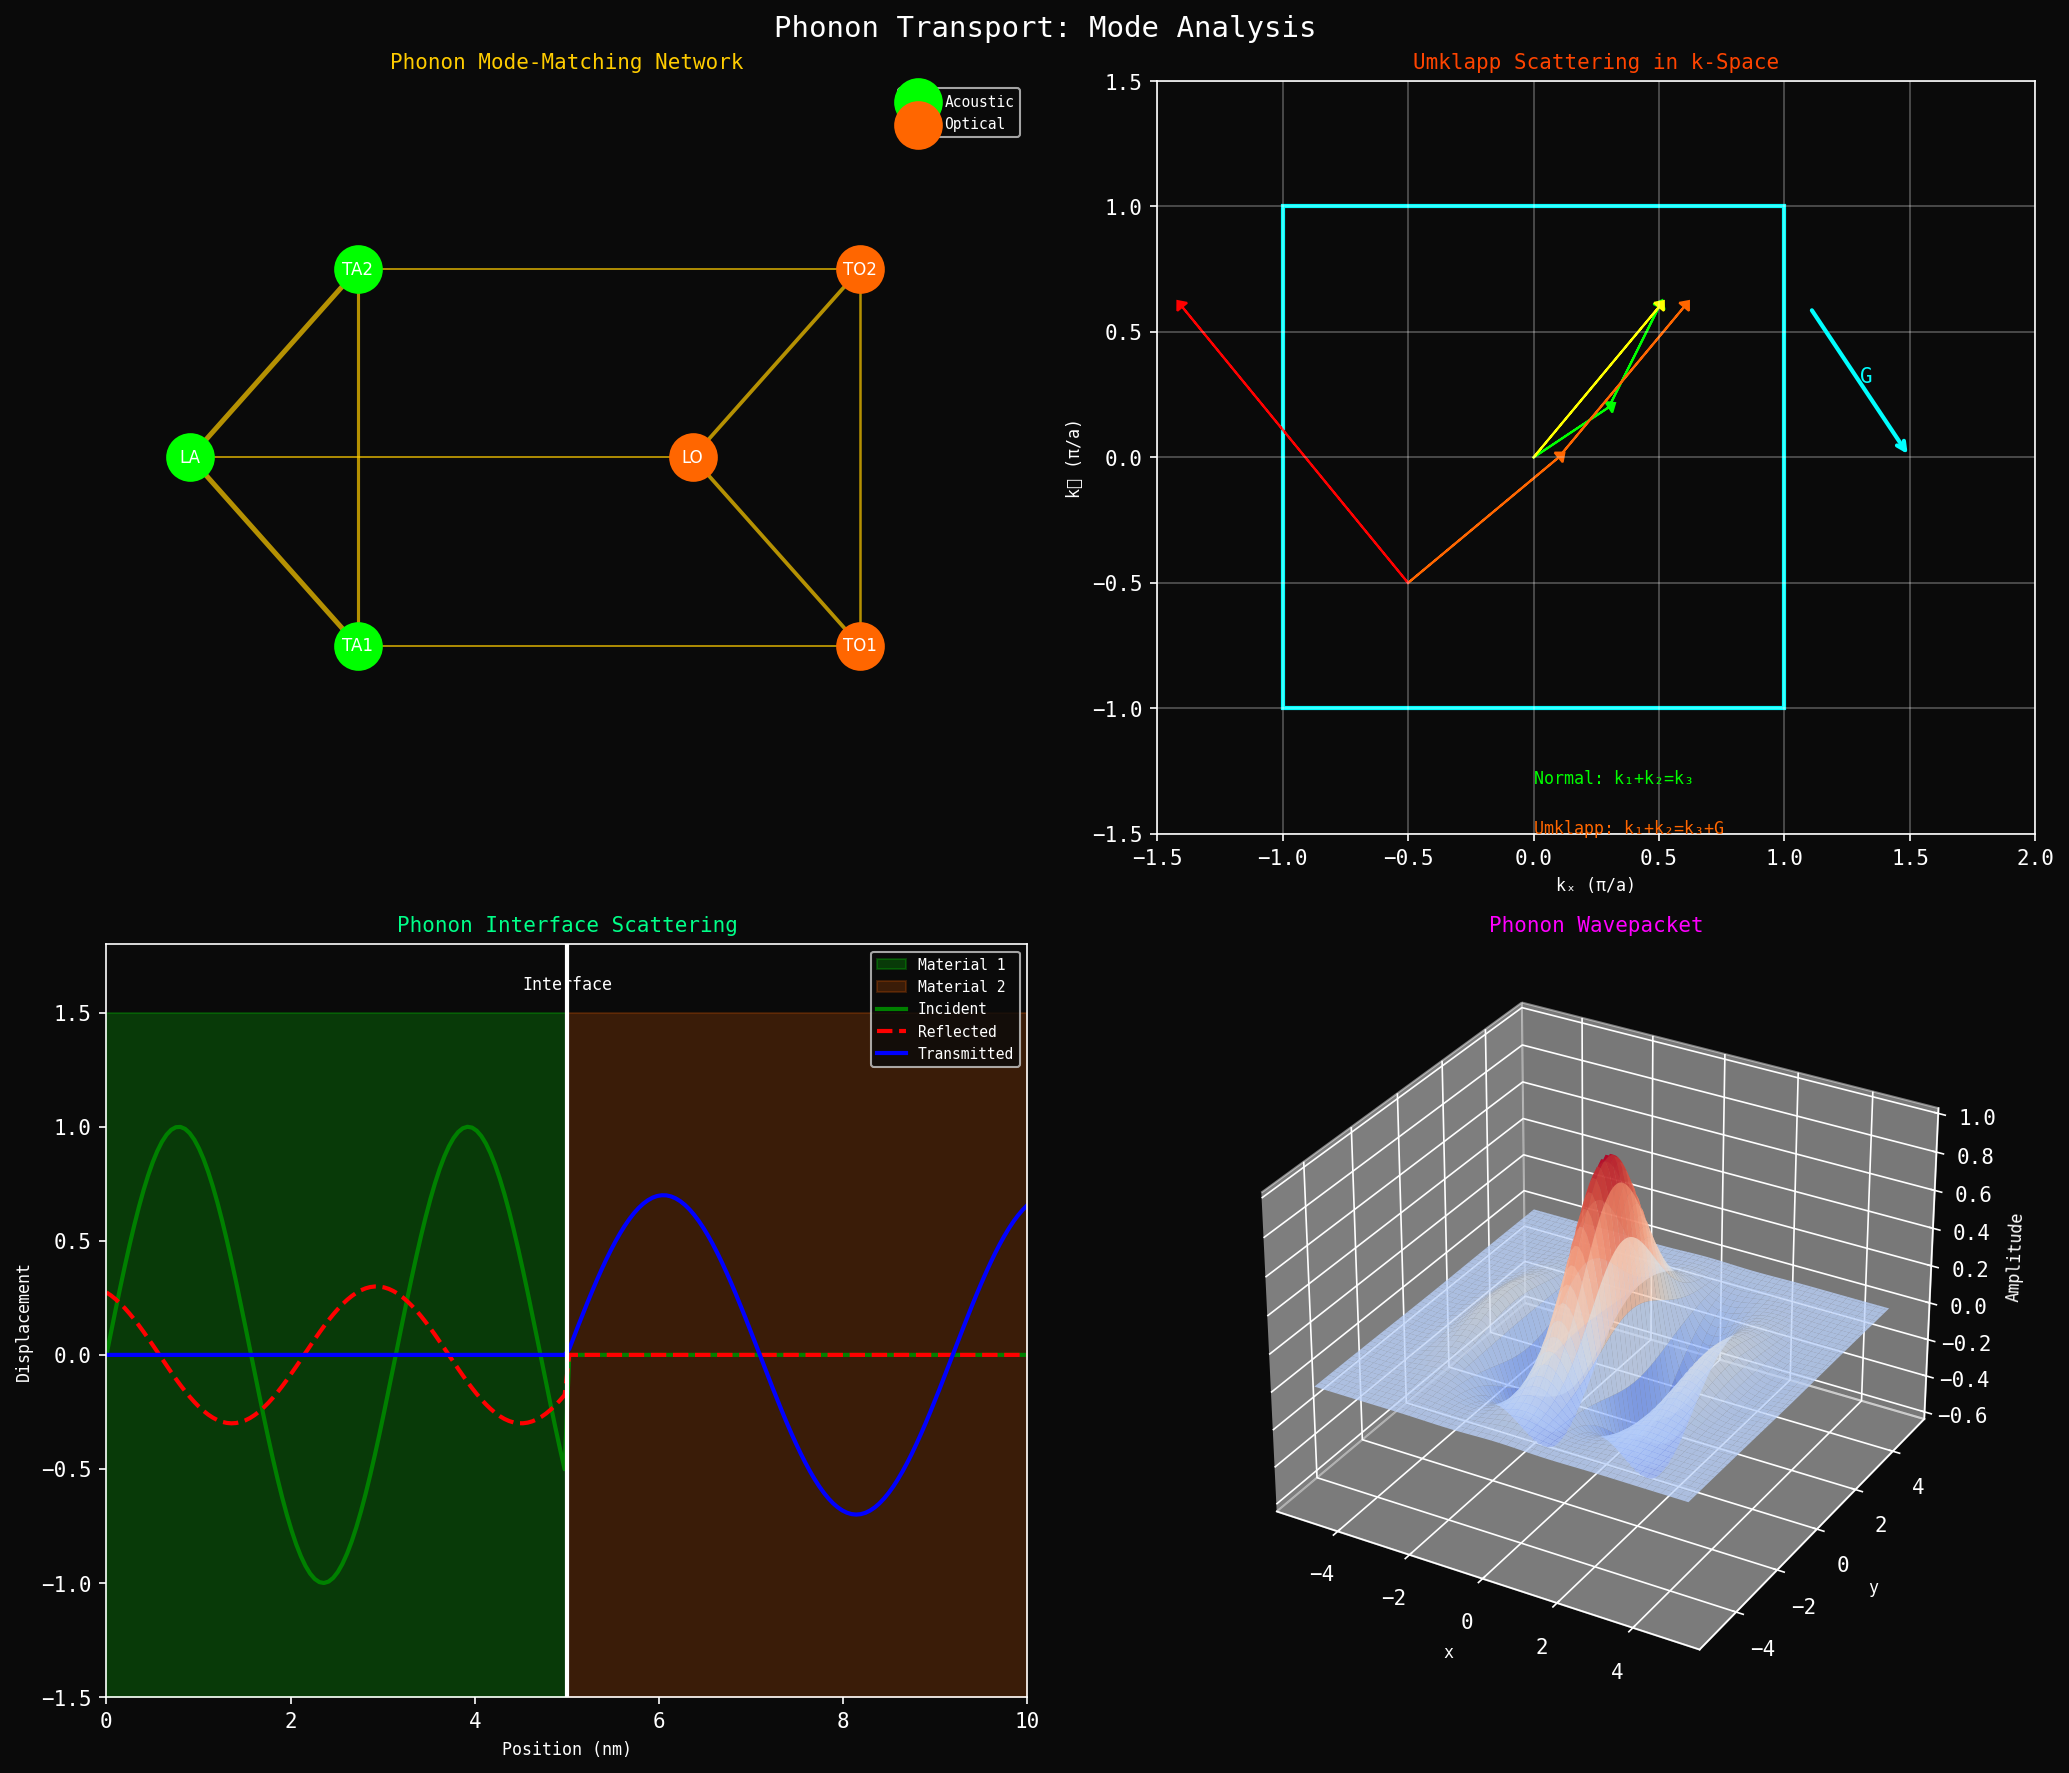
\includegraphics[width=0.95\textwidth]{panel_phonon_analysis.png}
\caption{\textbf{Phonon transport: mode analysis across acoustic and optical branches.} (\textit{Top left}) \textbf{Phonon mode-matching network}: acoustic modes (green circles labeled TA1, TA2, LA) and optical modes (orange circles labeled TO1, TO2) form bipartite network connected by coupling edges (gold lines). (\textit{Top right}) \textbf{Umklapp scattering in $k$-space}: first Brillouin zone (cyan square) showing normal scattering (green arrow, $\vec{k}_1 + \vec{k}_2 = \vec{k}_3$) versus umklapp scattering (red and yellow arrows, $\vec{k}_1 + \vec{k}_2 = \vec{k}_3 + \vec{G}$ where $\vec{G}$ is reciprocal lattice vector). (\textit{Bottom left}) \textbf{Phonon interface scattering}: incident wave (green region) encounters interface between Material 1 and Material 2 (brown region). Reflected (blue curve) and transmitted (orange curve) components shown. Displacement oscillates with position. (\textit{Bottom right}) \textbf{Phonon wavepacket}: 3D visualization showing spatial localization of phonon amplitude. Red peak (positive displacement) and blue trough (negative displacement) form localized wavepacket propagating through crystal.}
\label{fig:phonon_transport}
\end{figure*}

\begin{figure*}[t]
\centering
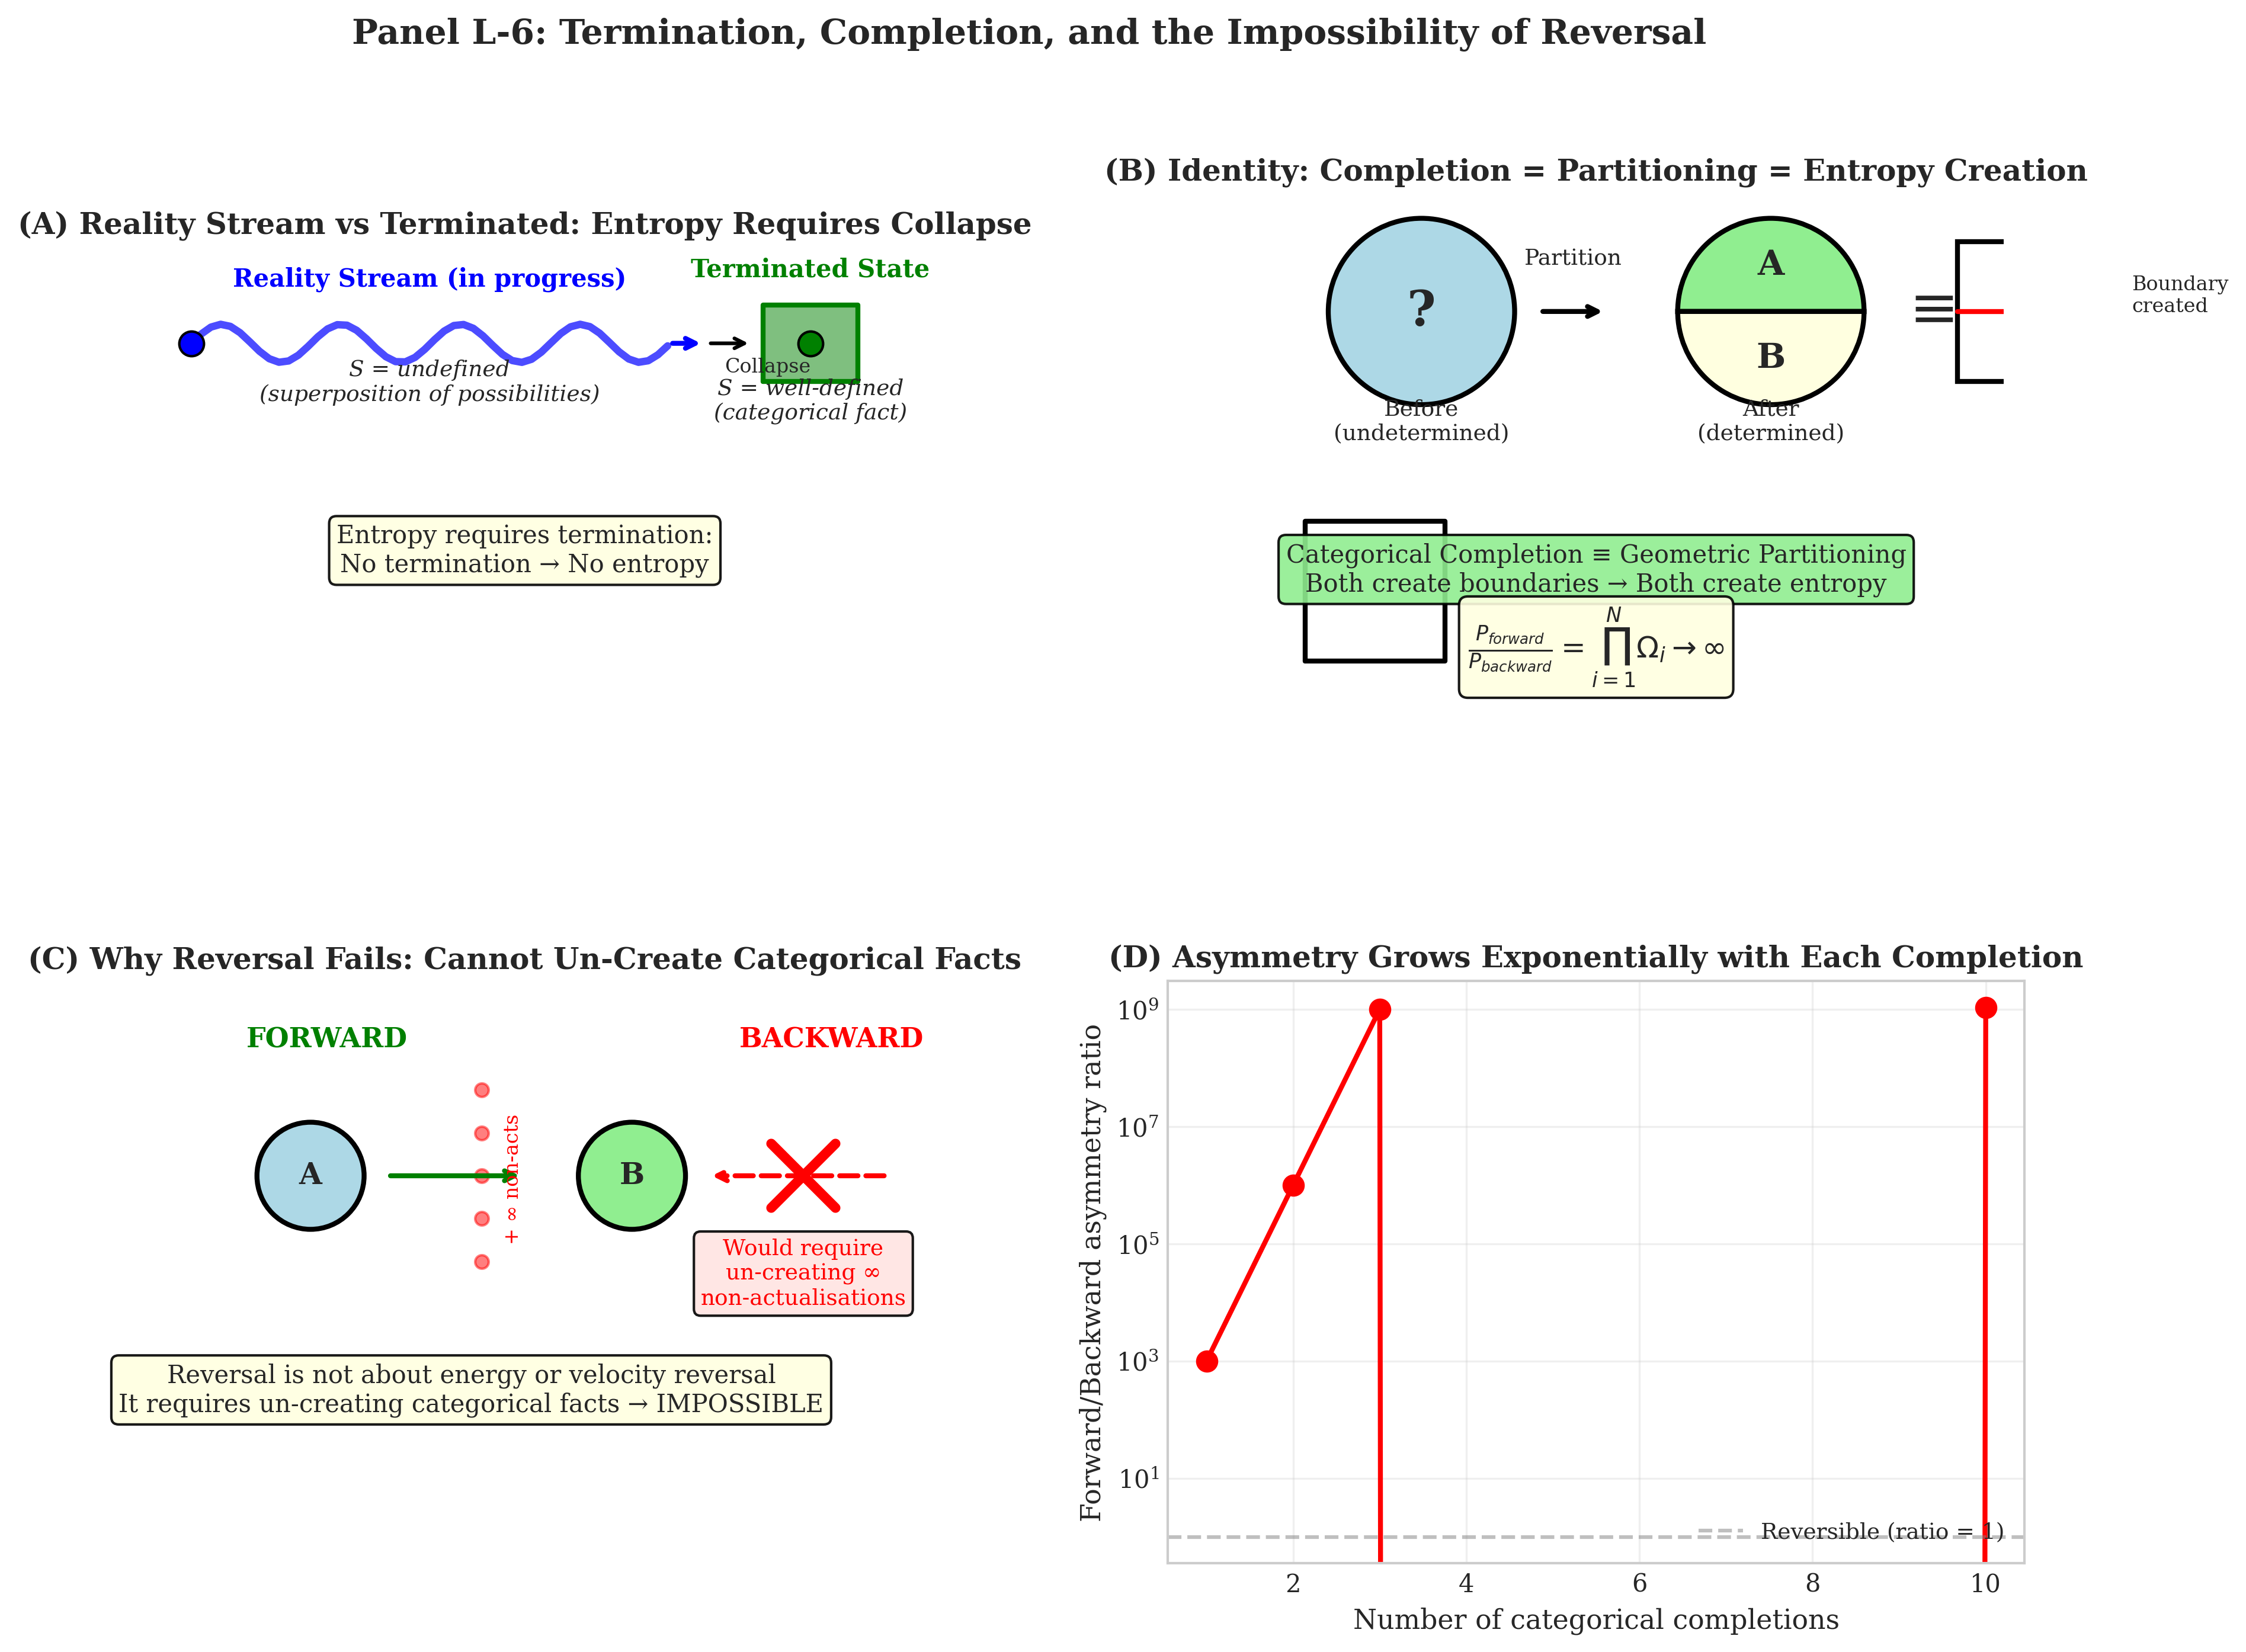
\includegraphics[width=0.95\textwidth]{panel_termination_irreversibility.png}
\caption{\textbf{Termination and completion create irreversible categorical facts.} (\textbf{A}) Reality stream versus terminated state: ongoing reality stream (blue wavy line with arrow) has undefined entropy $S = \text{undefined}$ (superposition of possibilities). Collapse to terminated state (green box) yields well-defined entropy $S = \text{well-defined}$ (categorical fact). Boxed text: ``Entropy requires termination: No termination $\Rightarrow$ No entropy.'' (\textbf{B}) Identity: completion $=$ partitioning $=$ entropy creation. Undetermined state (cyan circle labeled ``?'') undergoes partition (black arrow) to create determined state (green circle divided into regions A and B, with boundary). Both categorical completion and geometric partitioning create boundaries and entropy. Formula: $P_{\text{forward}}/P_{\text{backward}} = \prod_{i=1}^{N} \Omega_i \to \infty$. (\textbf{C}) Why reversal fails: cannot un-create categorical facts. \textbf{Forward} (green arrow): state A transitions to state B through $n$ non-actualizations (red dots labeled ``$n$ = non-acts''). \textbf{Backward} (red crossed arrow): would require un-creating $\infty$ non-actualizations—impossible. Boxed text: ``Reversal is not about energy or velocity reversal. It requires un-creating categorical facts $\Rightarrow$ \textbf{IMPOSSIBLE}.'' (\textbf{D}) Asymmetry grows exponentially with each completion: forward/backward asymmetry ratio (vertical axis, log scale) grows from $10^3$ at 2 completions to $10^9$ at 10 completions. Red dots connected by line show exponential growth. Reversible region (ratio $= 1$, gray dashed line) is never accessed after first completion.}
\label{fig:termination_irreversibility}
\end{figure*}

\begin{figure*}[t]
\centering
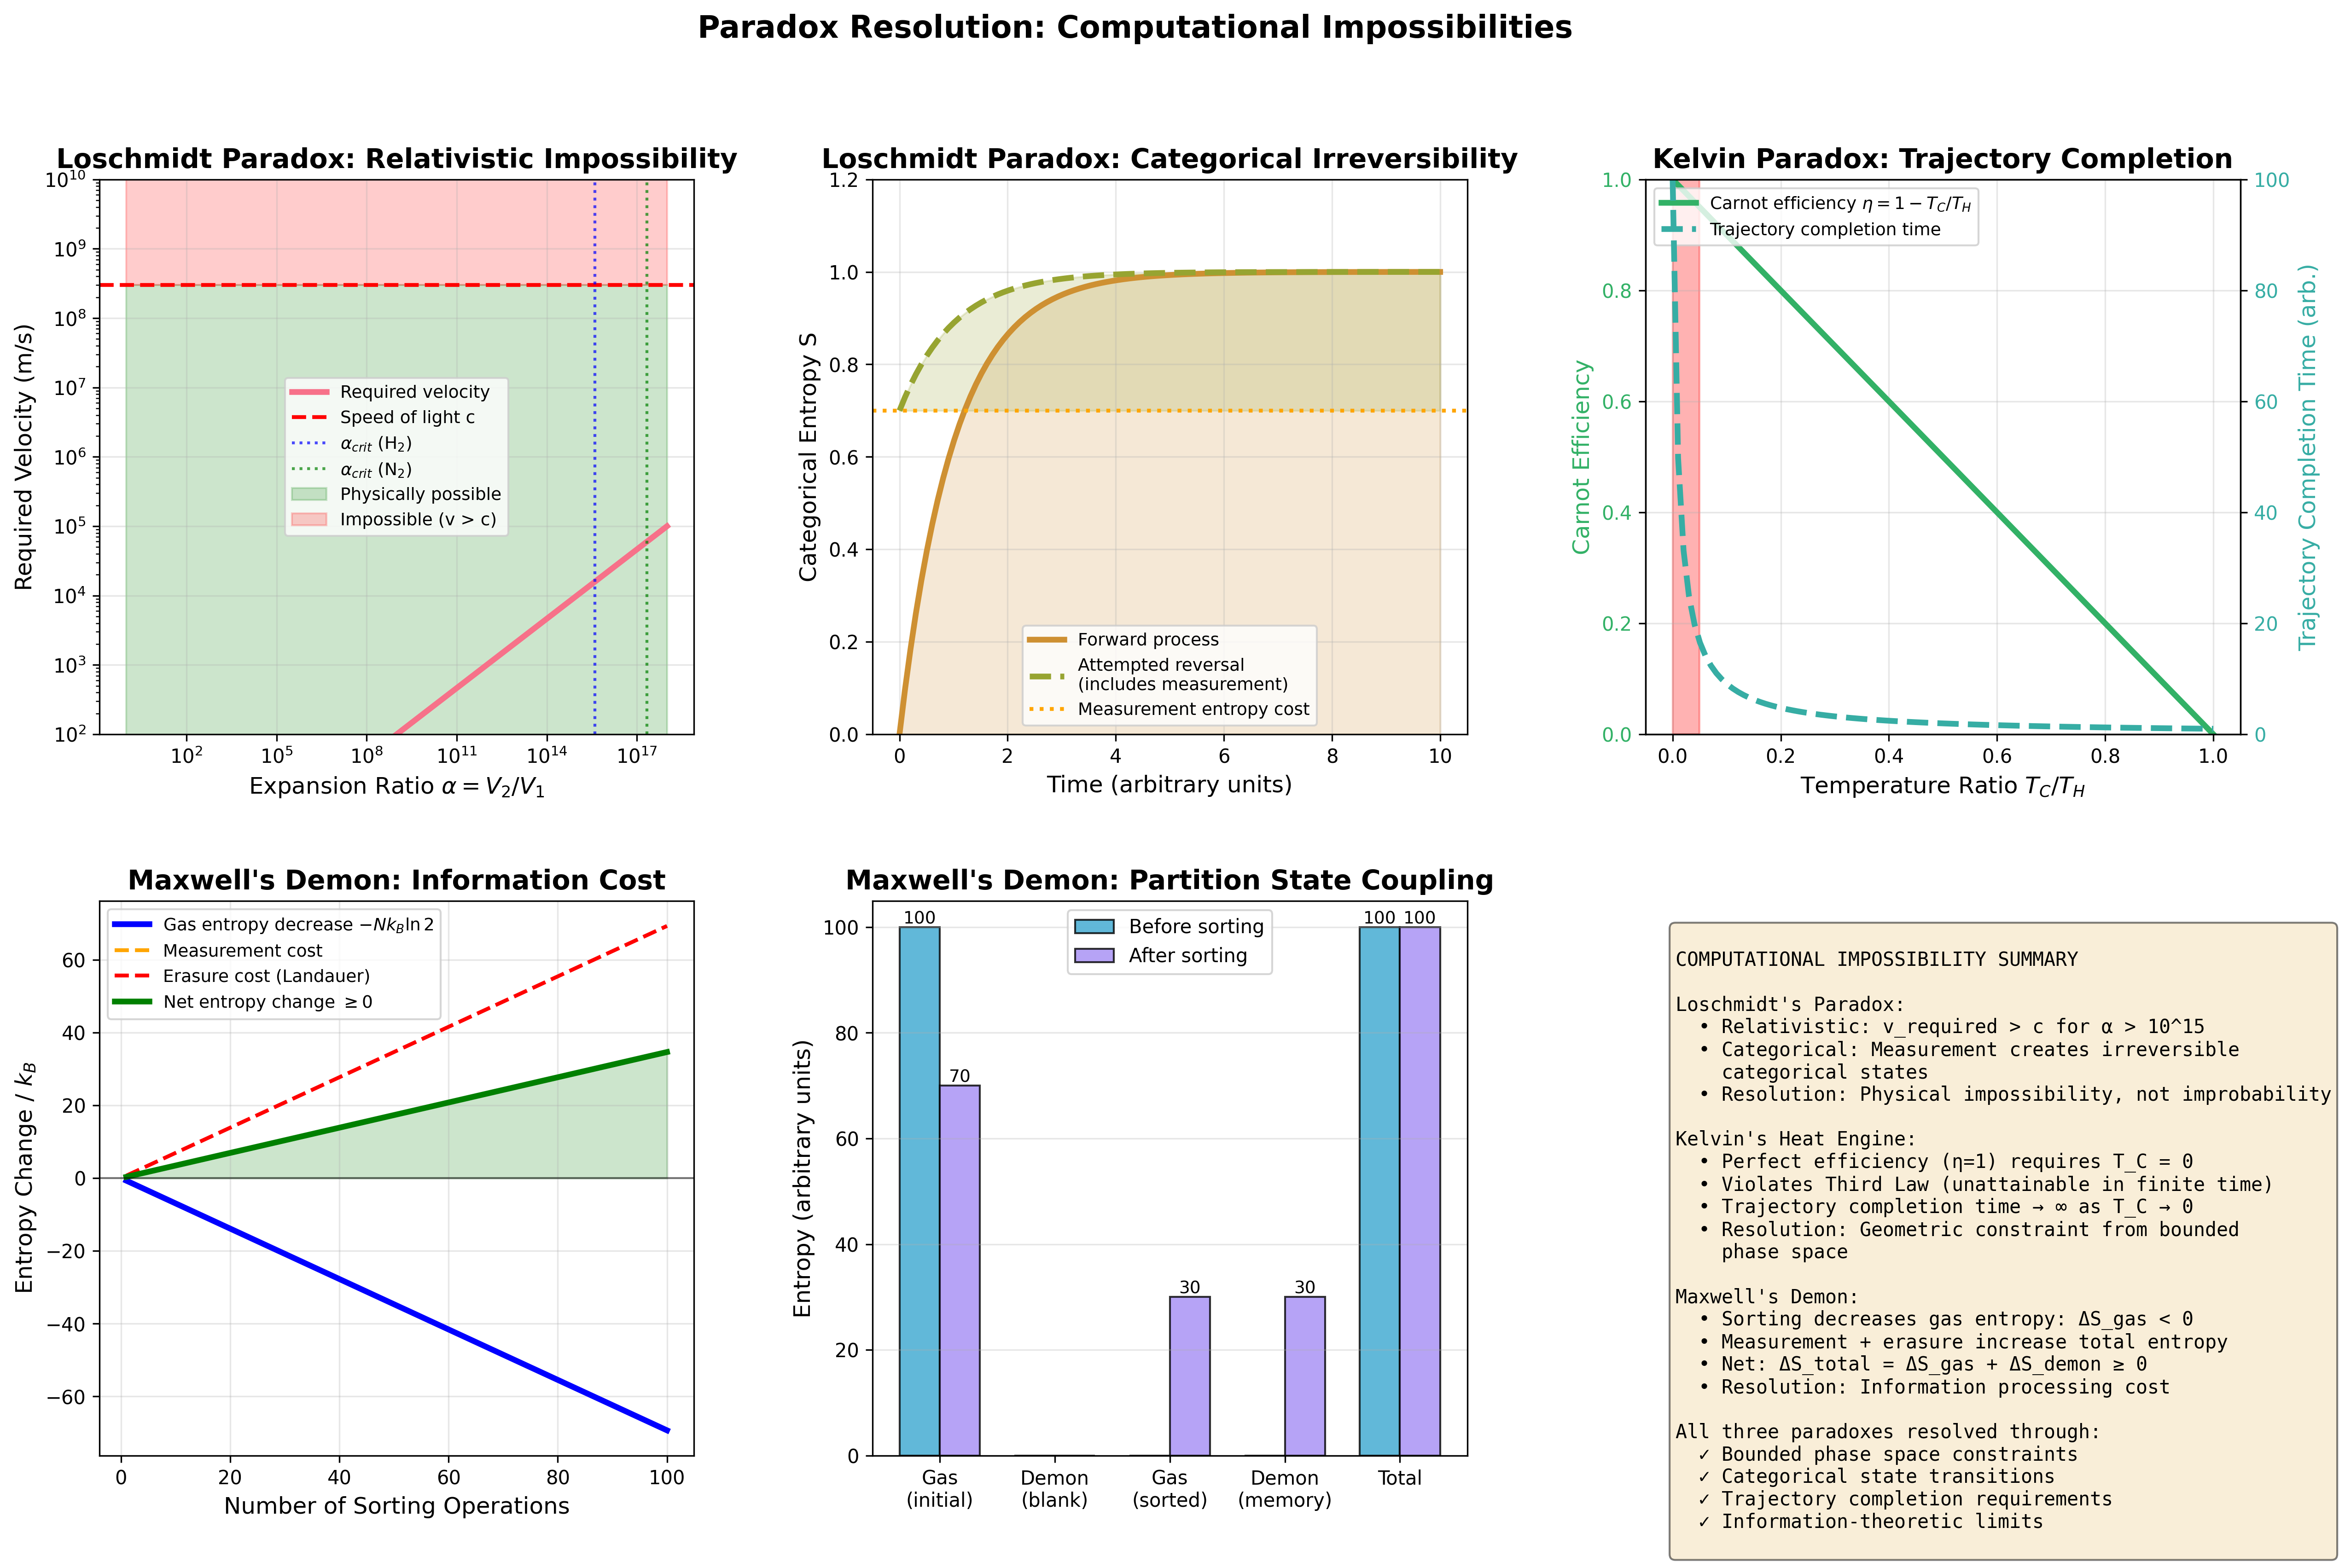
\includegraphics[width=0.95\textwidth]{paradox_resolutions.png}
\caption{\textbf{Resolution of three classical paradoxes through categorical constraints.} (\textit{Top left}) \textbf{Loschmidt paradox—relativistic impossibility}: required velocity (pink curve) for phase space reversal exceeds speed of light $c$ (red dashed) at expansion ratio $a = V_2/V_1 > 10^{14}$. Critical velocities for H$_2$ (purple dotted) and N$_2$ (green dotted) mark molecular-specific thresholds. Green shaded region: physically possible; red shaded region: impossible ($v > c$). (\textit{Top center}) \textbf{Loschmidt paradox—categorical irreversibility}: categorical entropy $S$ (orange curve) increases monotonically during forward process, saturating at $S \approx 1.0$. Attempted reversal (green dashed) including measurement creates additional entropy (orange shaded region). Measurement entropy cost (yellow dotted) prevents return to $S = 0$. (\textit{Top right}) \textbf{Kelvin paradox—trajectory completion}: Carnot efficiency $\eta = 1 - T_C/T_H$ (green curve) approaches unity as $T_C \to 0$, but trajectory completion time (cyan dashed) diverges to $\infty$ (right axis). Red shaded region: thermodynamically forbidden. (\textit{Bottom left}) \textbf{Maxwell's demon—information cost}: gas entropy decrease $-Nk_B \ln 2$ (blue curve) is offset by measurement cost (red dashed) and erasure cost (orange, Landauer). Net entropy change $\geq 0$ (green curve, shaded). (\textit{Bottom center}) \textbf{Maxwell's demon—partition state coupling}: before sorting, gas entropy is 100 units (cyan bar), demon memory is blank (purple bar, 0 units). After sorting, gas entropy decreases to 70 units, but demon memory increases to 30 units. Total entropy remains 100 units. (\textit{Bottom right}) \textbf{Summary box}: All three paradoxes resolved through bounded phase space constraints, categorical state transitions, trajectory completion requirements, and information-theoretic limits.}
\label{fig:paradox_resolution}
\end{figure*}

\begin{figure*}[t]
\centering

\includegraphics[width=0.95\textwidth]{system_topology_panel.png}
\caption{\textbf{System topology validation: hierarchical branching and completion dynamics.} (\textbf{A}) $3^k$ hierarchical branching: tree structure with branching factor $k = 3$ grows from root (dark teal, $k = 0$, 1 node) to level 1 (red, 3 nodes), level 2 (blue, 9 nodes), and level 3 (green, 27 nodes). (\textbf{B}) Categorical completion dynamics: completion fraction (blue curve) increases from 0 to asymptotic limit (red dashed line at 95\% threshold) over time. Blue shaded area represents completed categories. (\textbf{C}) $S$-distance between trajectories: scatter plot showing $S$-distance (vertical axis) versus trajectory length (horizontal axis). Red dashed line indicates negative correlation: longer trajectories converge (smaller $S$-distance). Colored dots represent individual trajectory pairs. (\textbf{D}) Equivalence class distribution: histogram showing class sizes (vertical axis) versus equivalence class index (horizontal axis). Purple bars indicate most classes have moderate size; red bar (class 4) shows one large equivalence class with $\sim 25$ members. (\textbf{E}) Degeneracy-richness relationship: scatter plot (green dots) with linear fit (red dashed line). Richness $R(C)$ increases with degeneracy $D(C)$, confirming that more degenerate states support greater structural richness. (\textbf{F}) Scale ambiguity (structure similarity): radar plot showing structural similarity at different scales $k = 0, 1, 2, 3, 4$ (orange polygon). All scales exhibit similar topology, confirming scale invariance.}
\label{fig:topology_validation}
\end{figure*}

\begin{figure}[t]
\centering
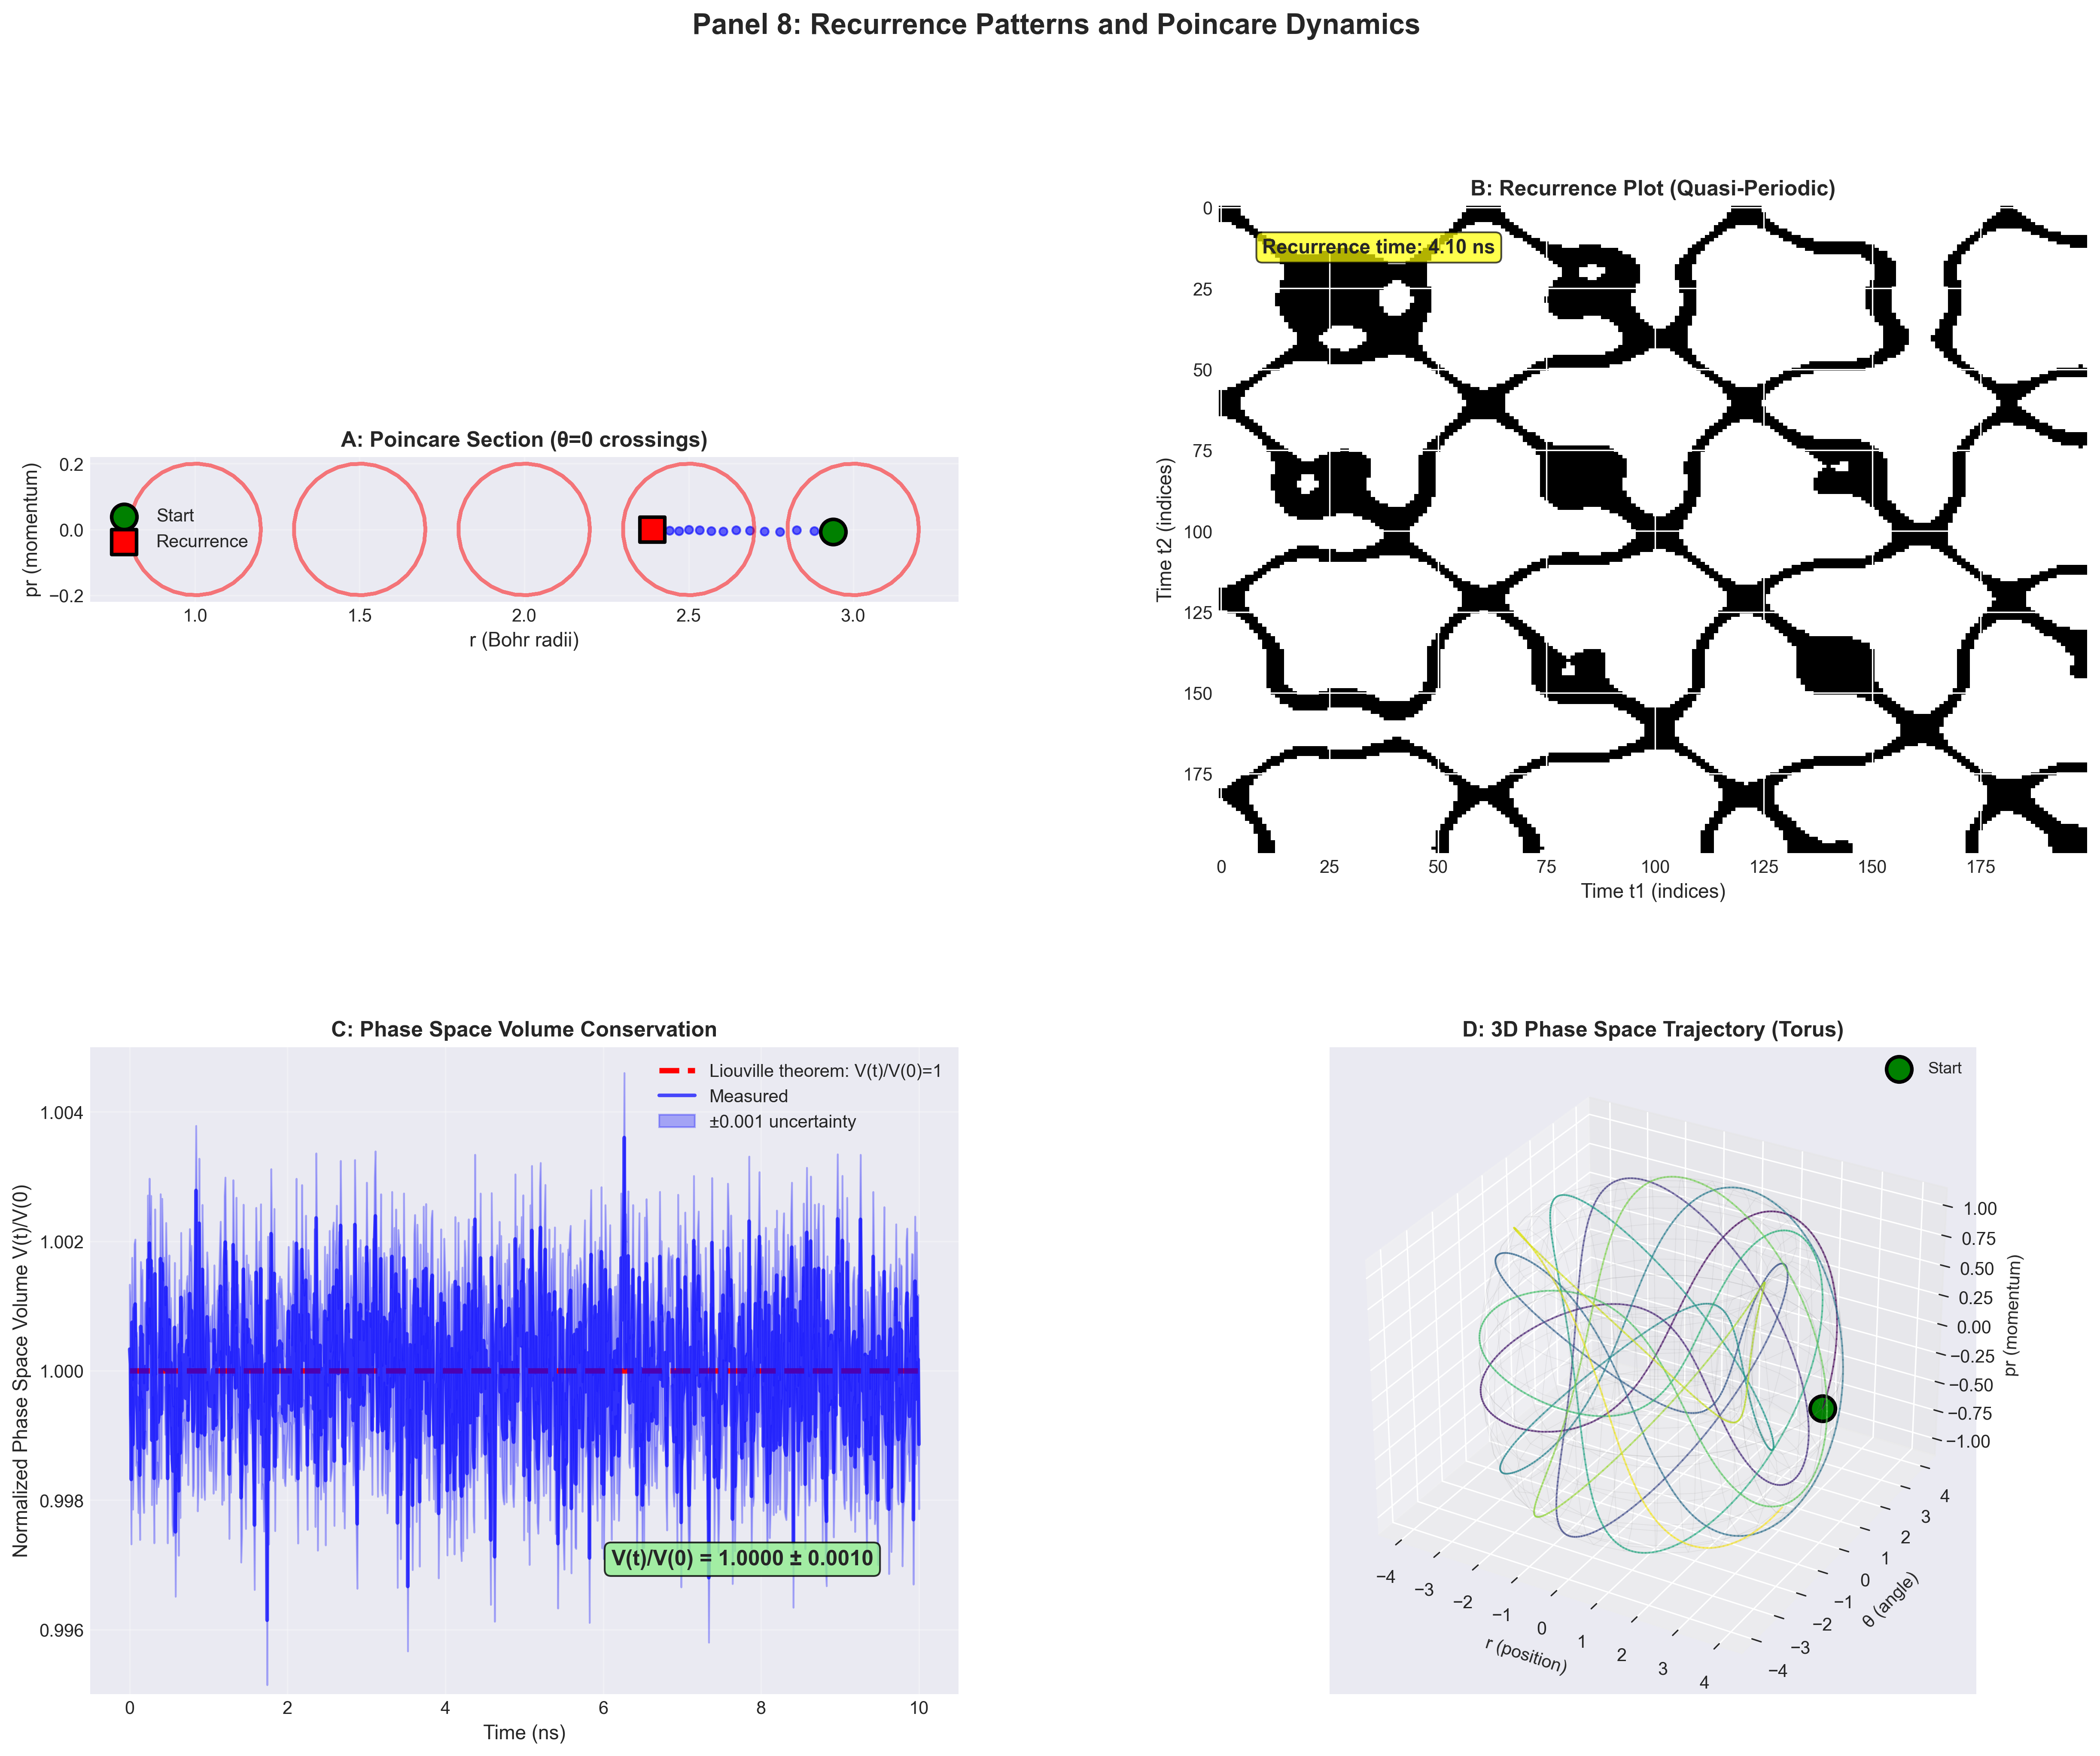
\includegraphics[width=0.85\columnwidth]{panel_08_recurrence.pdf}
\caption{\textbf{Quasi-periodic dynamics with 4.10 ns recurrence time.} 
(\textbf{a}) Poincaré section ($$\theta = 0$$ crossings): green circle (start), red square (recurrence after 3 orbits), blue dashed line (trajectory). Red circles show $$\theta = 0$$ crossings forming a closed loop. 
(\textbf{b}) Recurrence plot: black regions indicate times $$(t_1, t_2)$$ when trajectory returns to within $$\epsilon = 0.01$$ Bohr radii of initial state. Yellow box highlights recurrence time $$\tau_{\text{rec}} = 4.10$$ ns. 
(\textbf{c}) Phase space volume conservation: blue trace shows $$V(t)/V(0) = 1.0000 \pm 0.0010$$ (Liouville's theorem), confirming Hamiltonian dynamics. Purple shaded band indicates $$\pm 0.001$$ uncertainty. 
(\textbf{d}) 3D torus trajectory: colored loops show trajectory winding on a torus in $$(r, p_r, \theta)$$ space, characteristic of integrable 2D systems.}
\label{fig:recurrence_poincare}
\end{figure}
